\chapter{Generative Neural Networks}\label{chap:Arch1}
We use generative neural networks to generate denoised images from their noisy representation and thus solve the denoising problem. The class of generative network used to complete this task is a convolutional neural network. We introduces the notion of a \acl{CNN} and its components in section \ref{sec:Convolutional neural networks}, then section \ref{sec:Generative network architectures} goes over each specific network architecture we have worked with. All networks presented is this chapter are generative; a generative network takes an image of $W\times H$ pixels with three channels and generates a new image of the same dimensions. It differs from other types of \aclp{CNN} which have different output shapes, for example a classification network (such as those used in chapter \ref{chap:Arch2}) outputs one to a few probabilities, and segmentation networks usually have the same height and width dimensions as the input image but one channel per segmented feature (segmentation networks can easily be adapted into generative models as is the case for U-Net \cite{unet}). 

\section{Convolutional neural networks}\label{sec:Convolutional neural networks}
%- Introduce convolutional neural networks

We use deep convolutional neural networks which are neural networks based on the multilayer perceptron; that is, input data from one layer is sent to the neurons of the next layer and a dot product is performed between that input data and the next layer's learned weights. This process goes on for each layer. The main difference between a multilayer perceptron and a \ac{CNN} is that a \ac{CNN} is not fully connected so neurons in one layer only receive a subset of the previous layer's neurons. Instead, a \ac{CNN} takes advantage of the local spatial coherence of the input images to share weights and thus reduce the number of shared parameters. This process is shown in figure \ref{fig:convolutionfilter} where one filter is applied across the previous (in this case first) layer to create one channel of the following layer.

% plural?
The first and last layer of a generative network have the same shape as the input image, that is its height, width, and 3-channels representing the RGB color-space. Most layers in a deep network are hidden layers between the first and last one. Hidden layers contain many more channels (also called feature maps), they are usually convolution (or transposed convolution) layers, activation layers, or pooling layers.

A loss function is applied to the output of the last layer, its gradient with respect to the network's weights is calculated with the backpropagation algorithm, and the Adam gradient-descent algorithm\cite{adam} (the optimizer) adjusts the weights at the end of each batch training iteration. The optimizer's learning rate needs to be fine-tuned in order to optimize fast learning without over-fitting.

\subsection{Layers}

\begin{figure}
  \begin{center}
    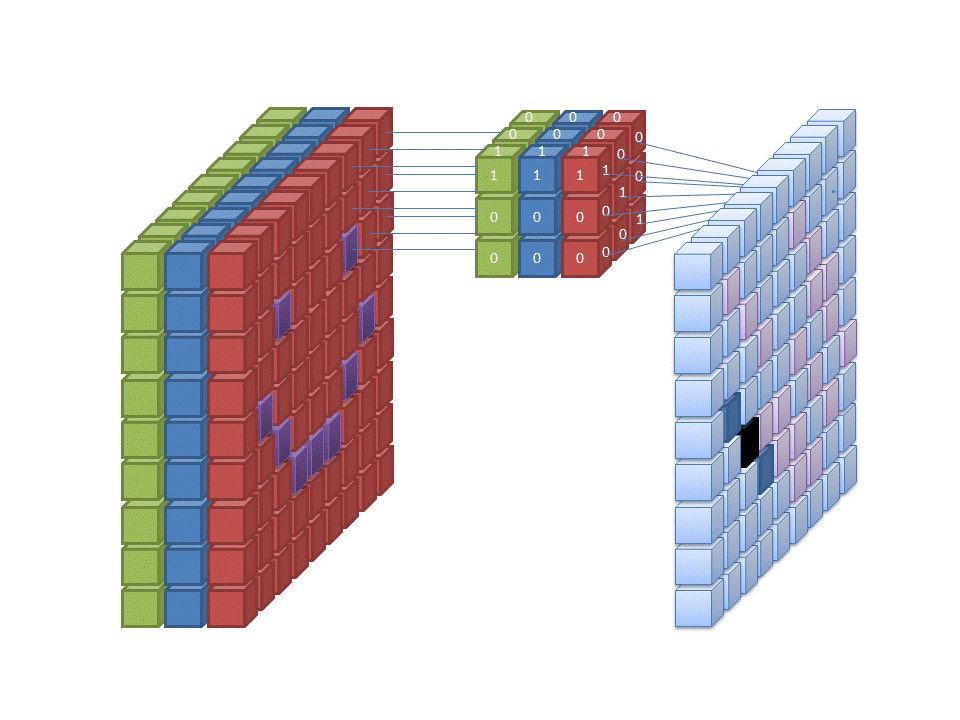
\includegraphics{gfx/Convolutional_Neural_Network_with_Color_Image_Filter.png}
    \caption[Standard convolution]{A filter is applied to the first 3-channels (RGB) input of an image in a convolutional neural network. The same filter is applied across all channels of the whole image as shown, and many of these filters are applied to form the following layer's feature map (i.e. its channels). Illustration by Wikimedia Commons user \href{https://commons.wikimedia.org/wiki/File:Convolutional_Neural_Network_with_Color_Image_Filter.gif}{Cecbur} (\href{https://creativecommons.org/licenses/by-sa/4.0/deed.en}{CC-BY-SA-4.0} license)}
    \label{fig:convolutionfilter}
  \end{center}
\end{figure}

\textbf{Convolution layers} apply convolutions with $C$ filters (also called features) to every $\acs{k}*\acs{k}$ area in the previous layer's width and height\footnote{assuming a stride of 1}, taking in every channel and returning one value per filter. Convolutions have a receptive field that is determined by \ac{k} whose typical values are 3 or 5. The next layer's width and height is thus reduced unless padding is applied. Given an input layer's width or height dimension $d$ and \ac{p}, a convolution layer's output size can be calculated as $d-\ac{k}+2\ac{p}+1$. Each filter is weighted and weights are learned parameters. The same stack of filters is applied on every $\ac{k}*\ac{k}$ area of a given layer; therefore, \acp{CNN} have largely reduced number of weight parameters.

\textbf{Activation layers} introduce non-linearity; they apply an activation function to every value in the previous layer and the resulting layer has the same shape as its input layer. We use the Sigmoid ($\phi(z)={1\over{1+e^{-z}}}$) which constrains its input values between 0 and 1, and (parametric) \ac{ReLU} ($R(z)=\max(0,z)$) as activation functions. 

% add gradient descent, BN

\subsection{Loss function}
% therefore and however are not interchangeable but they are used the same way with the punctuation sort of like that yeah they should never have as pace on either side words
The loss function assigns a score to the generated images with respect to the provided ground-truth. A loss function should not simply compare the difference between generated and ground-truth pixels because there is no one-to-one mapping between clean and noisy images. Therefore, a loss function which only focuses on the difference between pixels favors denoised images whose pixels average the many acceptable values; i.e. the network is trained to generate blurry images. \cite{pix2pix}

The \ac{MSE} (or $\ell 2$ loss) measures the average squared difference between the generated and ground-truth pixels \newline($MSE(\text{generated}, \text{ground-truth})=\sum_p^\text{pixels}{(\text{generated}_p-\text{ground-truth}_p)^2\over{|\text{pixels}|}}$), it is a simple yet effective loss function. Similarly, the $\ell 1$ loss measures the sum of the absolute differences between ground-truth and generated pixels; this typically favors blurrier results. The \ac{SSIM} index is another metric which puts weights on structural information that is more likely to be perceived in images, namely local changes in luminance, contrast, and structure. A loss may also be learned such as the discriminator in an \acl{GAN}.

%https://arxiv.org/pdf/1511.08861.pdf
Mixing different losses often appears to yield better results \cite{lossescomp}, although it is sometimes challenging to combine them because they are often scaled differently (and training may suffer a performance penalty when having to compute multiple losses). Another valid approach is to switch loss function once convergence has been attained with one. \cite{lossescomp} We typically use the \ac{SSIM} index in our standard models and a combination of loss functions in the more challenging \ac{GAN}.

%\marginpar{TODO: batch normalization}

\section{Generative network architectures}\label{sec:Generative network architectures}
\subsection{DnCNN}
DnCNN is a simple flat \ac{CNN} architecture introduced by Zhang et al. \cite{dncnn} to denoise images with residual learning. The network performs end-to-end denoising using only a convolution layer followed by \acl{BN} and a \ac{ReLU} activation layer at each depth level. The dimensions of the layers remain constant because the convolutions are padded appropriately ($\ac{p}={\ac{k}-1\over{2}}$). %The authors used a depth of 20 for blind gaussian denoising and set $\ac{k}=3$

The main contribution introduced in \cite{dncnn} appears to be the use of residual learning to speed up learning by modeling and subtracting the residual noise rather than generating a clean image. The use of a simple DnCNN architecture may have been introduced to emphasize the effectiveness of residual learning. DnCNN is the first network we experimented with because of its simplicity, and although most of our experiment focus on the subsequent networks, we tested the author's residual learning theory with our dataset of ISO noise in order to assess whether it would yield any gain in performance.
\subsection{RED-Net}
The \ac{RED-Net} architecture is a deep encoder-decoder network with residual skip connections \cite{rednet}. We found this type of network offers significantly better denoising performance and faster convergence than the DnCNN model. The first half of the network encodes the image using convolutions without padding such that the layers' dimensions continuously decrease, then the second half of the network (decoder) is made of transposed convolution layers that increase the layers' dimensions up to the original image's height and width. A \ac{ReLU} activation layer is placed between every (de)convolution layer. What is referred to as a residual network differs from the residual learning in Zhang et al. \cite{dncnn}. A residual network has skip connections which in the case of \ac{RED-Net} are placed every two convolution layers and connect them to transposed convolution layers of matching dimensions. These skip connections add details that may have been lost in the encoding process to the output of the transposed convolutions. 
\subsection{U-Net}
The U-Net architecture is an encoder-decoder with skip connections originally designed for image segmentation. Its use in an image generator is possible by using the number of input color channels as output features and upsampling the resulting image. Each U-Net block applies two 3x3 convolutions followed by a parameter-free pooling operation that downsamples the image by a factor of two. The first block has 64 filters and the number of filters doubles after every pooling operation until there are 1024 filters. From this point the downsampling pooling operations are replaced with 2x2 upsampling transposed convolutions and the number of filters get halved every time, but the convolutions remain (as opposed to using transposed convolutions) so the layers' size remain smaller on the upsampling stage than it is originally. This design results in corrupted borders which need to be discarded. The U-Net architecture uses significantly less resources than conventional encoder-decoder networks and it is able to capture details at multiple frequencies.
\subsection{HulbNet}\label{sec:HulbNet}
We designed a multi-scale architecture somewhat similar to U-Net whose aim is to be more adapted to the denoising problem at hand. HulbNet uses the following concepts:
\begin{figure}
  \begin{center}
    \animategraphics[width=\textwidth/3*2]{1}{gfx/dilation/frame-}{0}{8}
    \caption[Dilated convolution]{Dilated convolution (dilation=2). Illustration by GitHub user \href{https://github.com/vdumoulin/conv\_arithmetic}{vdumoulin} (\href{https://github.com/vdumoulin/conv\_arithmetic/blob/master/LICENSE}{MIT} license)}
    \label{fig:dilated}
  \end{center}
\end{figure}
\begin{figure}
  \begin{center}
  % Graphic for TeX using PGF
% Title: /orb/Dev/mthesis-denoise/thesis/gfx/convstr3.dia
% Creator: Dia v0.97.3
% CreationDate: Sun May 19 19:55:18 2019
% For: trougnouf
% \usepackage{tikz}
% The following commands are not supported in PSTricks at present
% We define them conditionally, so when they are implemented,
% this pgf file will use them.
\ifx\du\undefined
  \newlength{\du}
\fi
\setlength{\du}{15\unitlength}
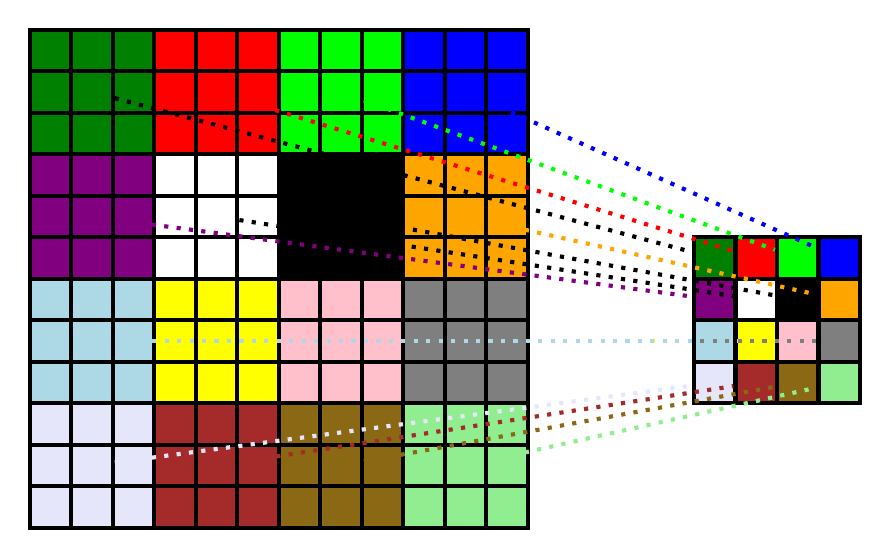
\begin{tikzpicture}
\pgftransformxscale{1.000000}
\pgftransformyscale{-1.000000}
\definecolor{dialinecolor}{rgb}{0.000000, 0.000000, 0.000000}
\pgfsetstrokecolor{dialinecolor}
\definecolor{dialinecolor}{rgb}{1.000000, 1.000000, 1.000000}
\pgfsetfillcolor{dialinecolor}
\pgfsetlinewidth{0.100000\du}
\pgfsetdash{}{0pt}
\pgfsetdash{}{0pt}
\pgfsetmiterjoin
\definecolor{dialinecolor}{rgb}{0.000000, 0.501961, 0.000000}
\pgfsetfillcolor{dialinecolor}
\fill (28.000000\du,10.000000\du)--(28.000000\du,11.000000\du)--(29.000000\du,11.000000\du)--(29.000000\du,10.000000\du)--cycle;
\definecolor{dialinecolor}{rgb}{0.000000, 0.000000, 0.000000}
\pgfsetstrokecolor{dialinecolor}
\draw (28.000000\du,10.000000\du)--(28.000000\du,11.000000\du)--(29.000000\du,11.000000\du)--(29.000000\du,10.000000\du)--cycle;
\pgfsetlinewidth{0.100000\du}
\pgfsetdash{}{0pt}
\pgfsetdash{}{0pt}
\pgfsetmiterjoin
\definecolor{dialinecolor}{rgb}{0.501961, 0.000000, 0.501961}
\pgfsetfillcolor{dialinecolor}
\fill (28.000000\du,11.000000\du)--(28.000000\du,12.000000\du)--(29.000000\du,12.000000\du)--(29.000000\du,11.000000\du)--cycle;
\definecolor{dialinecolor}{rgb}{0.000000, 0.000000, 0.000000}
\pgfsetstrokecolor{dialinecolor}
\draw (28.000000\du,11.000000\du)--(28.000000\du,12.000000\du)--(29.000000\du,12.000000\du)--(29.000000\du,11.000000\du)--cycle;
\pgfsetlinewidth{0.100000\du}
\pgfsetdash{}{0pt}
\pgfsetdash{}{0pt}
\pgfsetmiterjoin
\definecolor{dialinecolor}{rgb}{0.678431, 0.847059, 0.901961}
\pgfsetfillcolor{dialinecolor}
\fill (28.000000\du,12.000000\du)--(28.000000\du,13.000000\du)--(29.000000\du,13.000000\du)--(29.000000\du,12.000000\du)--cycle;
\definecolor{dialinecolor}{rgb}{0.000000, 0.000000, 0.000000}
\pgfsetstrokecolor{dialinecolor}
\draw (28.000000\du,12.000000\du)--(28.000000\du,13.000000\du)--(29.000000\du,13.000000\du)--(29.000000\du,12.000000\du)--cycle;
\pgfsetlinewidth{0.100000\du}
\pgfsetdash{}{0pt}
\pgfsetdash{}{0pt}
\pgfsetmiterjoin
\definecolor{dialinecolor}{rgb}{0.901961, 0.901961, 0.980392}
\pgfsetfillcolor{dialinecolor}
\fill (28.000000\du,13.000000\du)--(28.000000\du,14.000000\du)--(29.000000\du,14.000000\du)--(29.000000\du,13.000000\du)--cycle;
\definecolor{dialinecolor}{rgb}{0.000000, 0.000000, 0.000000}
\pgfsetstrokecolor{dialinecolor}
\draw (28.000000\du,13.000000\du)--(28.000000\du,14.000000\du)--(29.000000\du,14.000000\du)--(29.000000\du,13.000000\du)--cycle;
\pgfsetlinewidth{0.100000\du}
\pgfsetdash{}{0pt}
\pgfsetdash{}{0pt}
\pgfsetmiterjoin
\definecolor{dialinecolor}{rgb}{0.647059, 0.164706, 0.164706}
\pgfsetfillcolor{dialinecolor}
\fill (29.000000\du,13.000000\du)--(29.000000\du,14.000000\du)--(30.000000\du,14.000000\du)--(30.000000\du,13.000000\du)--cycle;
\definecolor{dialinecolor}{rgb}{0.000000, 0.000000, 0.000000}
\pgfsetstrokecolor{dialinecolor}
\draw (29.000000\du,13.000000\du)--(29.000000\du,14.000000\du)--(30.000000\du,14.000000\du)--(30.000000\du,13.000000\du)--cycle;
\pgfsetlinewidth{0.100000\du}
\pgfsetdash{}{0pt}
\pgfsetdash{}{0pt}
\pgfsetmiterjoin
\definecolor{dialinecolor}{rgb}{0.545098, 0.411765, 0.078431}
\pgfsetfillcolor{dialinecolor}
\fill (30.000000\du,13.000000\du)--(30.000000\du,14.000000\du)--(31.000000\du,14.000000\du)--(31.000000\du,13.000000\du)--cycle;
\definecolor{dialinecolor}{rgb}{0.000000, 0.000000, 0.000000}
\pgfsetstrokecolor{dialinecolor}
\draw (30.000000\du,13.000000\du)--(30.000000\du,14.000000\du)--(31.000000\du,14.000000\du)--(31.000000\du,13.000000\du)--cycle;
\pgfsetlinewidth{0.100000\du}
\pgfsetdash{}{0pt}
\pgfsetdash{}{0pt}
\pgfsetmiterjoin
\definecolor{dialinecolor}{rgb}{0.564706, 0.933333, 0.564706}
\pgfsetfillcolor{dialinecolor}
\fill (31.000000\du,13.000000\du)--(31.000000\du,14.000000\du)--(32.000000\du,14.000000\du)--(32.000000\du,13.000000\du)--cycle;
\definecolor{dialinecolor}{rgb}{0.000000, 0.000000, 0.000000}
\pgfsetstrokecolor{dialinecolor}
\draw (31.000000\du,13.000000\du)--(31.000000\du,14.000000\du)--(32.000000\du,14.000000\du)--(32.000000\du,13.000000\du)--cycle;
\pgfsetlinewidth{0.100000\du}
\pgfsetdash{}{0pt}
\pgfsetdash{}{0pt}
\pgfsetmiterjoin
\definecolor{dialinecolor}{rgb}{1.000000, 0.000000, 0.000000}
\pgfsetfillcolor{dialinecolor}
\fill (15.000000\du,5.000000\du)--(15.000000\du,6.000000\du)--(16.000000\du,6.000000\du)--(16.000000\du,5.000000\du)--cycle;
\definecolor{dialinecolor}{rgb}{0.000000, 0.000000, 0.000000}
\pgfsetstrokecolor{dialinecolor}
\draw (15.000000\du,5.000000\du)--(15.000000\du,6.000000\du)--(16.000000\du,6.000000\du)--(16.000000\du,5.000000\du)--cycle;
\pgfsetlinewidth{0.100000\du}
\pgfsetdash{}{0pt}
\pgfsetdash{}{0pt}
\pgfsetmiterjoin
\definecolor{dialinecolor}{rgb}{1.000000, 0.000000, 0.000000}
\pgfsetfillcolor{dialinecolor}
\fill (16.000000\du,5.000000\du)--(16.000000\du,6.000000\du)--(17.000000\du,6.000000\du)--(17.000000\du,5.000000\du)--cycle;
\definecolor{dialinecolor}{rgb}{0.000000, 0.000000, 0.000000}
\pgfsetstrokecolor{dialinecolor}
\draw (16.000000\du,5.000000\du)--(16.000000\du,6.000000\du)--(17.000000\du,6.000000\du)--(17.000000\du,5.000000\du)--cycle;
\pgfsetlinewidth{0.100000\du}
\pgfsetdash{}{0pt}
\pgfsetdash{}{0pt}
\pgfsetmiterjoin
\definecolor{dialinecolor}{rgb}{1.000000, 0.000000, 0.000000}
\pgfsetfillcolor{dialinecolor}
\fill (17.000000\du,5.000000\du)--(17.000000\du,6.000000\du)--(18.000000\du,6.000000\du)--(18.000000\du,5.000000\du)--cycle;
\definecolor{dialinecolor}{rgb}{0.000000, 0.000000, 0.000000}
\pgfsetstrokecolor{dialinecolor}
\draw (17.000000\du,5.000000\du)--(17.000000\du,6.000000\du)--(18.000000\du,6.000000\du)--(18.000000\du,5.000000\du)--cycle;
\pgfsetlinewidth{0.100000\du}
\pgfsetdash{}{0pt}
\pgfsetdash{}{0pt}
\pgfsetmiterjoin
\definecolor{dialinecolor}{rgb}{0.000000, 1.000000, 0.000000}
\pgfsetfillcolor{dialinecolor}
\fill (18.000000\du,5.000000\du)--(18.000000\du,6.000000\du)--(19.000000\du,6.000000\du)--(19.000000\du,5.000000\du)--cycle;
\definecolor{dialinecolor}{rgb}{0.000000, 0.000000, 0.000000}
\pgfsetstrokecolor{dialinecolor}
\draw (18.000000\du,5.000000\du)--(18.000000\du,6.000000\du)--(19.000000\du,6.000000\du)--(19.000000\du,5.000000\du)--cycle;
\pgfsetlinewidth{0.100000\du}
\pgfsetdash{}{0pt}
\pgfsetdash{}{0pt}
\pgfsetmiterjoin
\definecolor{dialinecolor}{rgb}{0.000000, 1.000000, 0.000000}
\pgfsetfillcolor{dialinecolor}
\fill (19.000000\du,5.000000\du)--(19.000000\du,6.000000\du)--(20.000000\du,6.000000\du)--(20.000000\du,5.000000\du)--cycle;
\definecolor{dialinecolor}{rgb}{0.000000, 0.000000, 0.000000}
\pgfsetstrokecolor{dialinecolor}
\draw (19.000000\du,5.000000\du)--(19.000000\du,6.000000\du)--(20.000000\du,6.000000\du)--(20.000000\du,5.000000\du)--cycle;
\pgfsetlinewidth{0.100000\du}
\pgfsetdash{}{0pt}
\pgfsetdash{}{0pt}
\pgfsetmiterjoin
\definecolor{dialinecolor}{rgb}{0.000000, 1.000000, 0.000000}
\pgfsetfillcolor{dialinecolor}
\fill (20.000000\du,5.000000\du)--(20.000000\du,6.000000\du)--(21.000000\du,6.000000\du)--(21.000000\du,5.000000\du)--cycle;
\definecolor{dialinecolor}{rgb}{0.000000, 0.000000, 0.000000}
\pgfsetstrokecolor{dialinecolor}
\draw (20.000000\du,5.000000\du)--(20.000000\du,6.000000\du)--(21.000000\du,6.000000\du)--(21.000000\du,5.000000\du)--cycle;
\pgfsetlinewidth{0.100000\du}
\pgfsetdash{}{0pt}
\pgfsetdash{}{0pt}
\pgfsetmiterjoin
\definecolor{dialinecolor}{rgb}{0.000000, 0.000000, 1.000000}
\pgfsetfillcolor{dialinecolor}
\fill (21.000000\du,5.000000\du)--(21.000000\du,6.000000\du)--(22.000000\du,6.000000\du)--(22.000000\du,5.000000\du)--cycle;
\definecolor{dialinecolor}{rgb}{0.000000, 0.000000, 0.000000}
\pgfsetstrokecolor{dialinecolor}
\draw (21.000000\du,5.000000\du)--(21.000000\du,6.000000\du)--(22.000000\du,6.000000\du)--(22.000000\du,5.000000\du)--cycle;
\pgfsetlinewidth{0.100000\du}
\pgfsetdash{}{0pt}
\pgfsetdash{}{0pt}
\pgfsetmiterjoin
\definecolor{dialinecolor}{rgb}{0.000000, 0.000000, 1.000000}
\pgfsetfillcolor{dialinecolor}
\fill (22.000000\du,5.000000\du)--(22.000000\du,6.000000\du)--(23.000000\du,6.000000\du)--(23.000000\du,5.000000\du)--cycle;
\definecolor{dialinecolor}{rgb}{0.000000, 0.000000, 0.000000}
\pgfsetstrokecolor{dialinecolor}
\draw (22.000000\du,5.000000\du)--(22.000000\du,6.000000\du)--(23.000000\du,6.000000\du)--(23.000000\du,5.000000\du)--cycle;
\pgfsetlinewidth{0.100000\du}
\pgfsetdash{}{0pt}
\pgfsetdash{}{0pt}
\pgfsetmiterjoin
\definecolor{dialinecolor}{rgb}{0.000000, 0.000000, 1.000000}
\pgfsetfillcolor{dialinecolor}
\fill (23.000000\du,5.000000\du)--(23.000000\du,6.000000\du)--(24.000000\du,6.000000\du)--(24.000000\du,5.000000\du)--cycle;
\definecolor{dialinecolor}{rgb}{0.000000, 0.000000, 0.000000}
\pgfsetstrokecolor{dialinecolor}
\draw (23.000000\du,5.000000\du)--(23.000000\du,6.000000\du)--(24.000000\du,6.000000\du)--(24.000000\du,5.000000\du)--cycle;
\pgfsetlinewidth{0.100000\du}
\pgfsetdash{}{0pt}
\pgfsetdash{}{0pt}
\pgfsetmiterjoin
\definecolor{dialinecolor}{rgb}{1.000000, 0.000000, 0.000000}
\pgfsetfillcolor{dialinecolor}
\fill (15.000000\du,6.000000\du)--(15.000000\du,7.000000\du)--(16.000000\du,7.000000\du)--(16.000000\du,6.000000\du)--cycle;
\definecolor{dialinecolor}{rgb}{0.000000, 0.000000, 0.000000}
\pgfsetstrokecolor{dialinecolor}
\draw (15.000000\du,6.000000\du)--(15.000000\du,7.000000\du)--(16.000000\du,7.000000\du)--(16.000000\du,6.000000\du)--cycle;
\pgfsetlinewidth{0.100000\du}
\pgfsetdash{}{0pt}
\pgfsetdash{}{0pt}
\pgfsetmiterjoin
\definecolor{dialinecolor}{rgb}{1.000000, 0.000000, 0.000000}
\pgfsetfillcolor{dialinecolor}
\fill (16.000000\du,6.000000\du)--(16.000000\du,7.000000\du)--(17.000000\du,7.000000\du)--(17.000000\du,6.000000\du)--cycle;
\definecolor{dialinecolor}{rgb}{0.000000, 0.000000, 0.000000}
\pgfsetstrokecolor{dialinecolor}
\draw (16.000000\du,6.000000\du)--(16.000000\du,7.000000\du)--(17.000000\du,7.000000\du)--(17.000000\du,6.000000\du)--cycle;
\pgfsetlinewidth{0.100000\du}
\pgfsetdash{}{0pt}
\pgfsetdash{}{0pt}
\pgfsetmiterjoin
\definecolor{dialinecolor}{rgb}{1.000000, 0.000000, 0.000000}
\pgfsetfillcolor{dialinecolor}
\fill (17.000000\du,6.000000\du)--(17.000000\du,7.000000\du)--(18.000000\du,7.000000\du)--(18.000000\du,6.000000\du)--cycle;
\definecolor{dialinecolor}{rgb}{0.000000, 0.000000, 0.000000}
\pgfsetstrokecolor{dialinecolor}
\draw (17.000000\du,6.000000\du)--(17.000000\du,7.000000\du)--(18.000000\du,7.000000\du)--(18.000000\du,6.000000\du)--cycle;
\pgfsetlinewidth{0.100000\du}
\pgfsetdash{}{0pt}
\pgfsetdash{}{0pt}
\pgfsetmiterjoin
\definecolor{dialinecolor}{rgb}{0.000000, 1.000000, 0.000000}
\pgfsetfillcolor{dialinecolor}
\fill (18.000000\du,6.000000\du)--(18.000000\du,7.000000\du)--(19.000000\du,7.000000\du)--(19.000000\du,6.000000\du)--cycle;
\definecolor{dialinecolor}{rgb}{0.000000, 0.000000, 0.000000}
\pgfsetstrokecolor{dialinecolor}
\draw (18.000000\du,6.000000\du)--(18.000000\du,7.000000\du)--(19.000000\du,7.000000\du)--(19.000000\du,6.000000\du)--cycle;
\pgfsetlinewidth{0.100000\du}
\pgfsetdash{}{0pt}
\pgfsetdash{}{0pt}
\pgfsetmiterjoin
\definecolor{dialinecolor}{rgb}{0.000000, 1.000000, 0.000000}
\pgfsetfillcolor{dialinecolor}
\fill (19.000000\du,6.000000\du)--(19.000000\du,7.000000\du)--(20.000000\du,7.000000\du)--(20.000000\du,6.000000\du)--cycle;
\definecolor{dialinecolor}{rgb}{0.000000, 0.000000, 0.000000}
\pgfsetstrokecolor{dialinecolor}
\draw (19.000000\du,6.000000\du)--(19.000000\du,7.000000\du)--(20.000000\du,7.000000\du)--(20.000000\du,6.000000\du)--cycle;
\pgfsetlinewidth{0.100000\du}
\pgfsetdash{}{0pt}
\pgfsetdash{}{0pt}
\pgfsetmiterjoin
\definecolor{dialinecolor}{rgb}{0.000000, 1.000000, 0.000000}
\pgfsetfillcolor{dialinecolor}
\fill (20.000000\du,6.000000\du)--(20.000000\du,7.000000\du)--(21.000000\du,7.000000\du)--(21.000000\du,6.000000\du)--cycle;
\definecolor{dialinecolor}{rgb}{0.000000, 0.000000, 0.000000}
\pgfsetstrokecolor{dialinecolor}
\draw (20.000000\du,6.000000\du)--(20.000000\du,7.000000\du)--(21.000000\du,7.000000\du)--(21.000000\du,6.000000\du)--cycle;
\pgfsetlinewidth{0.100000\du}
\pgfsetdash{}{0pt}
\pgfsetdash{}{0pt}
\pgfsetmiterjoin
\definecolor{dialinecolor}{rgb}{0.000000, 0.000000, 1.000000}
\pgfsetfillcolor{dialinecolor}
\fill (21.000000\du,6.000000\du)--(21.000000\du,7.000000\du)--(22.000000\du,7.000000\du)--(22.000000\du,6.000000\du)--cycle;
\definecolor{dialinecolor}{rgb}{0.000000, 0.000000, 0.000000}
\pgfsetstrokecolor{dialinecolor}
\draw (21.000000\du,6.000000\du)--(21.000000\du,7.000000\du)--(22.000000\du,7.000000\du)--(22.000000\du,6.000000\du)--cycle;
\pgfsetlinewidth{0.100000\du}
\pgfsetdash{}{0pt}
\pgfsetdash{}{0pt}
\pgfsetmiterjoin
\definecolor{dialinecolor}{rgb}{0.000000, 0.000000, 1.000000}
\pgfsetfillcolor{dialinecolor}
\fill (22.000000\du,6.000000\du)--(22.000000\du,7.000000\du)--(23.000000\du,7.000000\du)--(23.000000\du,6.000000\du)--cycle;
\definecolor{dialinecolor}{rgb}{0.000000, 0.000000, 0.000000}
\pgfsetstrokecolor{dialinecolor}
\draw (22.000000\du,6.000000\du)--(22.000000\du,7.000000\du)--(23.000000\du,7.000000\du)--(23.000000\du,6.000000\du)--cycle;
\pgfsetlinewidth{0.100000\du}
\pgfsetdash{}{0pt}
\pgfsetdash{}{0pt}
\pgfsetmiterjoin
\definecolor{dialinecolor}{rgb}{0.000000, 0.000000, 1.000000}
\pgfsetfillcolor{dialinecolor}
\fill (23.000000\du,6.000000\du)--(23.000000\du,7.000000\du)--(24.000000\du,7.000000\du)--(24.000000\du,6.000000\du)--cycle;
\definecolor{dialinecolor}{rgb}{0.000000, 0.000000, 0.000000}
\pgfsetstrokecolor{dialinecolor}
\draw (23.000000\du,6.000000\du)--(23.000000\du,7.000000\du)--(24.000000\du,7.000000\du)--(24.000000\du,6.000000\du)--cycle;
\pgfsetlinewidth{0.100000\du}
\pgfsetdash{}{0pt}
\pgfsetdash{}{0pt}
\pgfsetmiterjoin
\definecolor{dialinecolor}{rgb}{1.000000, 0.000000, 0.000000}
\pgfsetfillcolor{dialinecolor}
\fill (15.000000\du,7.000000\du)--(15.000000\du,8.000000\du)--(16.000000\du,8.000000\du)--(16.000000\du,7.000000\du)--cycle;
\definecolor{dialinecolor}{rgb}{0.000000, 0.000000, 0.000000}
\pgfsetstrokecolor{dialinecolor}
\draw (15.000000\du,7.000000\du)--(15.000000\du,8.000000\du)--(16.000000\du,8.000000\du)--(16.000000\du,7.000000\du)--cycle;
\pgfsetlinewidth{0.100000\du}
\pgfsetdash{}{0pt}
\pgfsetdash{}{0pt}
\pgfsetmiterjoin
\definecolor{dialinecolor}{rgb}{1.000000, 0.000000, 0.000000}
\pgfsetfillcolor{dialinecolor}
\fill (16.000000\du,7.000000\du)--(16.000000\du,8.000000\du)--(17.000000\du,8.000000\du)--(17.000000\du,7.000000\du)--cycle;
\definecolor{dialinecolor}{rgb}{0.000000, 0.000000, 0.000000}
\pgfsetstrokecolor{dialinecolor}
\draw (16.000000\du,7.000000\du)--(16.000000\du,8.000000\du)--(17.000000\du,8.000000\du)--(17.000000\du,7.000000\du)--cycle;
\pgfsetlinewidth{0.100000\du}
\pgfsetdash{}{0pt}
\pgfsetdash{}{0pt}
\pgfsetmiterjoin
\definecolor{dialinecolor}{rgb}{1.000000, 0.000000, 0.000000}
\pgfsetfillcolor{dialinecolor}
\fill (17.000000\du,7.000000\du)--(17.000000\du,8.000000\du)--(18.000000\du,8.000000\du)--(18.000000\du,7.000000\du)--cycle;
\definecolor{dialinecolor}{rgb}{0.000000, 0.000000, 0.000000}
\pgfsetstrokecolor{dialinecolor}
\draw (17.000000\du,7.000000\du)--(17.000000\du,8.000000\du)--(18.000000\du,8.000000\du)--(18.000000\du,7.000000\du)--cycle;
\pgfsetlinewidth{0.100000\du}
\pgfsetdash{}{0pt}
\pgfsetdash{}{0pt}
\pgfsetmiterjoin
\definecolor{dialinecolor}{rgb}{0.000000, 1.000000, 0.000000}
\pgfsetfillcolor{dialinecolor}
\fill (18.000000\du,7.000000\du)--(18.000000\du,8.000000\du)--(19.000000\du,8.000000\du)--(19.000000\du,7.000000\du)--cycle;
\definecolor{dialinecolor}{rgb}{0.000000, 0.000000, 0.000000}
\pgfsetstrokecolor{dialinecolor}
\draw (18.000000\du,7.000000\du)--(18.000000\du,8.000000\du)--(19.000000\du,8.000000\du)--(19.000000\du,7.000000\du)--cycle;
\pgfsetlinewidth{0.100000\du}
\pgfsetdash{}{0pt}
\pgfsetdash{}{0pt}
\pgfsetmiterjoin
\definecolor{dialinecolor}{rgb}{0.000000, 1.000000, 0.000000}
\pgfsetfillcolor{dialinecolor}
\fill (19.000000\du,7.000000\du)--(19.000000\du,8.000000\du)--(20.000000\du,8.000000\du)--(20.000000\du,7.000000\du)--cycle;
\definecolor{dialinecolor}{rgb}{0.000000, 0.000000, 0.000000}
\pgfsetstrokecolor{dialinecolor}
\draw (19.000000\du,7.000000\du)--(19.000000\du,8.000000\du)--(20.000000\du,8.000000\du)--(20.000000\du,7.000000\du)--cycle;
\pgfsetlinewidth{0.100000\du}
\pgfsetdash{}{0pt}
\pgfsetdash{}{0pt}
\pgfsetmiterjoin
\definecolor{dialinecolor}{rgb}{0.000000, 1.000000, 0.000000}
\pgfsetfillcolor{dialinecolor}
\fill (20.000000\du,7.000000\du)--(20.000000\du,8.000000\du)--(21.000000\du,8.000000\du)--(21.000000\du,7.000000\du)--cycle;
\definecolor{dialinecolor}{rgb}{0.000000, 0.000000, 0.000000}
\pgfsetstrokecolor{dialinecolor}
\draw (20.000000\du,7.000000\du)--(20.000000\du,8.000000\du)--(21.000000\du,8.000000\du)--(21.000000\du,7.000000\du)--cycle;
\pgfsetlinewidth{0.100000\du}
\pgfsetdash{}{0pt}
\pgfsetdash{}{0pt}
\pgfsetmiterjoin
\definecolor{dialinecolor}{rgb}{0.000000, 0.000000, 1.000000}
\pgfsetfillcolor{dialinecolor}
\fill (21.000000\du,7.000000\du)--(21.000000\du,8.000000\du)--(22.000000\du,8.000000\du)--(22.000000\du,7.000000\du)--cycle;
\definecolor{dialinecolor}{rgb}{0.000000, 0.000000, 0.000000}
\pgfsetstrokecolor{dialinecolor}
\draw (21.000000\du,7.000000\du)--(21.000000\du,8.000000\du)--(22.000000\du,8.000000\du)--(22.000000\du,7.000000\du)--cycle;
\pgfsetlinewidth{0.100000\du}
\pgfsetdash{}{0pt}
\pgfsetdash{}{0pt}
\pgfsetmiterjoin
\definecolor{dialinecolor}{rgb}{0.000000, 0.000000, 1.000000}
\pgfsetfillcolor{dialinecolor}
\fill (22.000000\du,7.000000\du)--(22.000000\du,8.000000\du)--(23.000000\du,8.000000\du)--(23.000000\du,7.000000\du)--cycle;
\definecolor{dialinecolor}{rgb}{0.000000, 0.000000, 0.000000}
\pgfsetstrokecolor{dialinecolor}
\draw (22.000000\du,7.000000\du)--(22.000000\du,8.000000\du)--(23.000000\du,8.000000\du)--(23.000000\du,7.000000\du)--cycle;
\pgfsetlinewidth{0.100000\du}
\pgfsetdash{}{0pt}
\pgfsetdash{}{0pt}
\pgfsetmiterjoin
\definecolor{dialinecolor}{rgb}{0.000000, 0.000000, 1.000000}
\pgfsetfillcolor{dialinecolor}
\fill (23.000000\du,7.000000\du)--(23.000000\du,8.000000\du)--(24.000000\du,8.000000\du)--(24.000000\du,7.000000\du)--cycle;
\definecolor{dialinecolor}{rgb}{0.000000, 0.000000, 0.000000}
\pgfsetstrokecolor{dialinecolor}
\draw (23.000000\du,7.000000\du)--(23.000000\du,8.000000\du)--(24.000000\du,8.000000\du)--(24.000000\du,7.000000\du)--cycle;
\pgfsetlinewidth{0.100000\du}
\pgfsetdash{}{0pt}
\pgfsetdash{}{0pt}
\pgfsetmiterjoin
\definecolor{dialinecolor}{rgb}{1.000000, 1.000000, 1.000000}
\pgfsetfillcolor{dialinecolor}
\fill (15.000000\du,8.000000\du)--(15.000000\du,9.000000\du)--(16.000000\du,9.000000\du)--(16.000000\du,8.000000\du)--cycle;
\definecolor{dialinecolor}{rgb}{0.000000, 0.000000, 0.000000}
\pgfsetstrokecolor{dialinecolor}
\draw (15.000000\du,8.000000\du)--(15.000000\du,9.000000\du)--(16.000000\du,9.000000\du)--(16.000000\du,8.000000\du)--cycle;
\pgfsetlinewidth{0.100000\du}
\pgfsetdash{}{0pt}
\pgfsetdash{}{0pt}
\pgfsetmiterjoin
\definecolor{dialinecolor}{rgb}{1.000000, 1.000000, 1.000000}
\pgfsetfillcolor{dialinecolor}
\fill (16.000000\du,8.000000\du)--(16.000000\du,9.000000\du)--(17.000000\du,9.000000\du)--(17.000000\du,8.000000\du)--cycle;
\definecolor{dialinecolor}{rgb}{0.000000, 0.000000, 0.000000}
\pgfsetstrokecolor{dialinecolor}
\draw (16.000000\du,8.000000\du)--(16.000000\du,9.000000\du)--(17.000000\du,9.000000\du)--(17.000000\du,8.000000\du)--cycle;
\pgfsetlinewidth{0.100000\du}
\pgfsetdash{}{0pt}
\pgfsetdash{}{0pt}
\pgfsetmiterjoin
\definecolor{dialinecolor}{rgb}{1.000000, 1.000000, 1.000000}
\pgfsetfillcolor{dialinecolor}
\fill (17.000000\du,8.000000\du)--(17.000000\du,9.000000\du)--(18.000000\du,9.000000\du)--(18.000000\du,8.000000\du)--cycle;
\definecolor{dialinecolor}{rgb}{0.000000, 0.000000, 0.000000}
\pgfsetstrokecolor{dialinecolor}
\draw (17.000000\du,8.000000\du)--(17.000000\du,9.000000\du)--(18.000000\du,9.000000\du)--(18.000000\du,8.000000\du)--cycle;
\pgfsetlinewidth{0.100000\du}
\pgfsetdash{}{0pt}
\pgfsetdash{}{0pt}
\pgfsetmiterjoin
\definecolor{dialinecolor}{rgb}{0.000000, 0.000000, 0.000000}
\pgfsetstrokecolor{dialinecolor}
\draw (18.000000\du,8.000000\du)--(18.000000\du,9.000000\du)--(19.000000\du,9.000000\du)--(19.000000\du,8.000000\du)--cycle;
\pgfsetlinewidth{0.100000\du}
\pgfsetdash{}{0pt}
\pgfsetdash{}{0pt}
\pgfsetmiterjoin
\definecolor{dialinecolor}{rgb}{0.000000, 0.000000, 0.000000}
\pgfsetfillcolor{dialinecolor}
\fill (18.000000\du,8.000000\du)--(18.000000\du,9.000000\du)--(19.000000\du,9.000000\du)--(19.000000\du,8.000000\du)--cycle;
\definecolor{dialinecolor}{rgb}{0.000000, 0.000000, 0.000000}
\pgfsetstrokecolor{dialinecolor}
\draw (18.000000\du,8.000000\du)--(18.000000\du,9.000000\du)--(19.000000\du,9.000000\du)--(19.000000\du,8.000000\du)--cycle;
\pgfsetlinewidth{0.100000\du}
\pgfsetdash{}{0pt}
\pgfsetdash{}{0pt}
\pgfsetmiterjoin
\definecolor{dialinecolor}{rgb}{0.000000, 0.000000, 0.000000}
\pgfsetfillcolor{dialinecolor}
\fill (20.000000\du,8.000000\du)--(20.000000\du,9.000000\du)--(21.000000\du,9.000000\du)--(21.000000\du,8.000000\du)--cycle;
\definecolor{dialinecolor}{rgb}{0.000000, 0.000000, 0.000000}
\pgfsetstrokecolor{dialinecolor}
\draw (20.000000\du,8.000000\du)--(20.000000\du,9.000000\du)--(21.000000\du,9.000000\du)--(21.000000\du,8.000000\du)--cycle;
\pgfsetlinewidth{0.100000\du}
\pgfsetdash{}{0pt}
\pgfsetdash{}{0pt}
\pgfsetmiterjoin
\definecolor{dialinecolor}{rgb}{1.000000, 0.647059, 0.000000}
\pgfsetfillcolor{dialinecolor}
\fill (21.000000\du,8.000000\du)--(21.000000\du,9.000000\du)--(22.000000\du,9.000000\du)--(22.000000\du,8.000000\du)--cycle;
\definecolor{dialinecolor}{rgb}{0.000000, 0.000000, 0.000000}
\pgfsetstrokecolor{dialinecolor}
\draw (21.000000\du,8.000000\du)--(21.000000\du,9.000000\du)--(22.000000\du,9.000000\du)--(22.000000\du,8.000000\du)--cycle;
\pgfsetlinewidth{0.100000\du}
\pgfsetdash{}{0pt}
\pgfsetdash{}{0pt}
\pgfsetmiterjoin
\definecolor{dialinecolor}{rgb}{1.000000, 0.647059, 0.000000}
\pgfsetfillcolor{dialinecolor}
\fill (22.000000\du,8.000000\du)--(22.000000\du,9.000000\du)--(23.000000\du,9.000000\du)--(23.000000\du,8.000000\du)--cycle;
\definecolor{dialinecolor}{rgb}{0.000000, 0.000000, 0.000000}
\pgfsetstrokecolor{dialinecolor}
\draw (22.000000\du,8.000000\du)--(22.000000\du,9.000000\du)--(23.000000\du,9.000000\du)--(23.000000\du,8.000000\du)--cycle;
\pgfsetlinewidth{0.100000\du}
\pgfsetdash{}{0pt}
\pgfsetdash{}{0pt}
\pgfsetmiterjoin
\definecolor{dialinecolor}{rgb}{1.000000, 0.647059, 0.000000}
\pgfsetfillcolor{dialinecolor}
\fill (23.000000\du,8.000000\du)--(23.000000\du,9.000000\du)--(24.000000\du,9.000000\du)--(24.000000\du,8.000000\du)--cycle;
\definecolor{dialinecolor}{rgb}{0.000000, 0.000000, 0.000000}
\pgfsetstrokecolor{dialinecolor}
\draw (23.000000\du,8.000000\du)--(23.000000\du,9.000000\du)--(24.000000\du,9.000000\du)--(24.000000\du,8.000000\du)--cycle;
\pgfsetlinewidth{0.100000\du}
\pgfsetdash{}{0pt}
\pgfsetdash{}{0pt}
\pgfsetmiterjoin
\definecolor{dialinecolor}{rgb}{1.000000, 1.000000, 1.000000}
\pgfsetfillcolor{dialinecolor}
\fill (15.000000\du,9.000000\du)--(15.000000\du,10.000000\du)--(16.000000\du,10.000000\du)--(16.000000\du,9.000000\du)--cycle;
\definecolor{dialinecolor}{rgb}{0.000000, 0.000000, 0.000000}
\pgfsetstrokecolor{dialinecolor}
\draw (15.000000\du,9.000000\du)--(15.000000\du,10.000000\du)--(16.000000\du,10.000000\du)--(16.000000\du,9.000000\du)--cycle;
\pgfsetlinewidth{0.100000\du}
\pgfsetdash{}{0pt}
\pgfsetdash{}{0pt}
\pgfsetmiterjoin
\definecolor{dialinecolor}{rgb}{1.000000, 1.000000, 1.000000}
\pgfsetfillcolor{dialinecolor}
\fill (16.000000\du,9.000000\du)--(16.000000\du,10.000000\du)--(17.000000\du,10.000000\du)--(17.000000\du,9.000000\du)--cycle;
\definecolor{dialinecolor}{rgb}{0.000000, 0.000000, 0.000000}
\pgfsetstrokecolor{dialinecolor}
\draw (16.000000\du,9.000000\du)--(16.000000\du,10.000000\du)--(17.000000\du,10.000000\du)--(17.000000\du,9.000000\du)--cycle;
\pgfsetlinewidth{0.100000\du}
\pgfsetdash{}{0pt}
\pgfsetdash{}{0pt}
\pgfsetmiterjoin
\definecolor{dialinecolor}{rgb}{1.000000, 1.000000, 1.000000}
\pgfsetfillcolor{dialinecolor}
\fill (17.000000\du,9.000000\du)--(17.000000\du,10.000000\du)--(18.000000\du,10.000000\du)--(18.000000\du,9.000000\du)--cycle;
\definecolor{dialinecolor}{rgb}{0.000000, 0.000000, 0.000000}
\pgfsetstrokecolor{dialinecolor}
\draw (17.000000\du,9.000000\du)--(17.000000\du,10.000000\du)--(18.000000\du,10.000000\du)--(18.000000\du,9.000000\du)--cycle;
\pgfsetlinewidth{0.100000\du}
\pgfsetdash{}{0pt}
\pgfsetdash{}{0pt}
\pgfsetmiterjoin
\definecolor{dialinecolor}{rgb}{0.000000, 0.000000, 0.000000}
\pgfsetfillcolor{dialinecolor}
\fill (18.000000\du,9.000000\du)--(18.000000\du,10.000000\du)--(19.000000\du,10.000000\du)--(19.000000\du,9.000000\du)--cycle;
\definecolor{dialinecolor}{rgb}{0.000000, 0.000000, 0.000000}
\pgfsetstrokecolor{dialinecolor}
\draw (18.000000\du,9.000000\du)--(18.000000\du,10.000000\du)--(19.000000\du,10.000000\du)--(19.000000\du,9.000000\du)--cycle;
\pgfsetlinewidth{0.100000\du}
\pgfsetdash{}{0pt}
\pgfsetdash{}{0pt}
\pgfsetmiterjoin
\definecolor{dialinecolor}{rgb}{0.000000, 0.000000, 0.000000}
\pgfsetfillcolor{dialinecolor}
\fill (19.000000\du,9.000000\du)--(19.000000\du,10.000000\du)--(20.000000\du,10.000000\du)--(20.000000\du,9.000000\du)--cycle;
\definecolor{dialinecolor}{rgb}{0.000000, 0.000000, 0.000000}
\pgfsetstrokecolor{dialinecolor}
\draw (19.000000\du,9.000000\du)--(19.000000\du,10.000000\du)--(20.000000\du,10.000000\du)--(20.000000\du,9.000000\du)--cycle;
\pgfsetlinewidth{0.100000\du}
\pgfsetdash{}{0pt}
\pgfsetdash{}{0pt}
\pgfsetmiterjoin
\definecolor{dialinecolor}{rgb}{0.000000, 0.000000, 0.000000}
\pgfsetfillcolor{dialinecolor}
\fill (20.000000\du,9.000000\du)--(20.000000\du,10.000000\du)--(21.000000\du,10.000000\du)--(21.000000\du,9.000000\du)--cycle;
\definecolor{dialinecolor}{rgb}{0.000000, 0.000000, 0.000000}
\pgfsetstrokecolor{dialinecolor}
\draw (20.000000\du,9.000000\du)--(20.000000\du,10.000000\du)--(21.000000\du,10.000000\du)--(21.000000\du,9.000000\du)--cycle;
\pgfsetlinewidth{0.100000\du}
\pgfsetdash{}{0pt}
\pgfsetdash{}{0pt}
\pgfsetmiterjoin
\definecolor{dialinecolor}{rgb}{1.000000, 0.647059, 0.000000}
\pgfsetfillcolor{dialinecolor}
\fill (21.000000\du,9.000000\du)--(21.000000\du,10.000000\du)--(22.000000\du,10.000000\du)--(22.000000\du,9.000000\du)--cycle;
\definecolor{dialinecolor}{rgb}{0.000000, 0.000000, 0.000000}
\pgfsetstrokecolor{dialinecolor}
\draw (21.000000\du,9.000000\du)--(21.000000\du,10.000000\du)--(22.000000\du,10.000000\du)--(22.000000\du,9.000000\du)--cycle;
\pgfsetlinewidth{0.100000\du}
\pgfsetdash{}{0pt}
\pgfsetdash{}{0pt}
\pgfsetmiterjoin
\definecolor{dialinecolor}{rgb}{1.000000, 0.647059, 0.000000}
\pgfsetfillcolor{dialinecolor}
\fill (22.000000\du,9.000000\du)--(22.000000\du,10.000000\du)--(23.000000\du,10.000000\du)--(23.000000\du,9.000000\du)--cycle;
\definecolor{dialinecolor}{rgb}{0.000000, 0.000000, 0.000000}
\pgfsetstrokecolor{dialinecolor}
\draw (22.000000\du,9.000000\du)--(22.000000\du,10.000000\du)--(23.000000\du,10.000000\du)--(23.000000\du,9.000000\du)--cycle;
\pgfsetlinewidth{0.100000\du}
\pgfsetdash{}{0pt}
\pgfsetdash{}{0pt}
\pgfsetmiterjoin
\definecolor{dialinecolor}{rgb}{1.000000, 0.647059, 0.000000}
\pgfsetfillcolor{dialinecolor}
\fill (23.000000\du,9.000000\du)--(23.000000\du,10.000000\du)--(24.000000\du,10.000000\du)--(24.000000\du,9.000000\du)--cycle;
\definecolor{dialinecolor}{rgb}{0.000000, 0.000000, 0.000000}
\pgfsetstrokecolor{dialinecolor}
\draw (23.000000\du,9.000000\du)--(23.000000\du,10.000000\du)--(24.000000\du,10.000000\du)--(24.000000\du,9.000000\du)--cycle;
\pgfsetlinewidth{0.100000\du}
\pgfsetdash{}{0pt}
\pgfsetdash{}{0pt}
\pgfsetmiterjoin
\definecolor{dialinecolor}{rgb}{1.000000, 1.000000, 1.000000}
\pgfsetfillcolor{dialinecolor}
\fill (15.000000\du,10.000000\du)--(15.000000\du,11.000000\du)--(16.000000\du,11.000000\du)--(16.000000\du,10.000000\du)--cycle;
\definecolor{dialinecolor}{rgb}{0.000000, 0.000000, 0.000000}
\pgfsetstrokecolor{dialinecolor}
\draw (15.000000\du,10.000000\du)--(15.000000\du,11.000000\du)--(16.000000\du,11.000000\du)--(16.000000\du,10.000000\du)--cycle;
\pgfsetlinewidth{0.100000\du}
\pgfsetdash{}{0pt}
\pgfsetdash{}{0pt}
\pgfsetmiterjoin
\definecolor{dialinecolor}{rgb}{1.000000, 1.000000, 1.000000}
\pgfsetfillcolor{dialinecolor}
\fill (16.000000\du,10.000000\du)--(16.000000\du,11.000000\du)--(17.000000\du,11.000000\du)--(17.000000\du,10.000000\du)--cycle;
\definecolor{dialinecolor}{rgb}{0.000000, 0.000000, 0.000000}
\pgfsetstrokecolor{dialinecolor}
\draw (16.000000\du,10.000000\du)--(16.000000\du,11.000000\du)--(17.000000\du,11.000000\du)--(17.000000\du,10.000000\du)--cycle;
\pgfsetlinewidth{0.100000\du}
\pgfsetdash{}{0pt}
\pgfsetdash{}{0pt}
\pgfsetmiterjoin
\definecolor{dialinecolor}{rgb}{1.000000, 1.000000, 1.000000}
\pgfsetfillcolor{dialinecolor}
\fill (17.000000\du,10.000000\du)--(17.000000\du,11.000000\du)--(18.000000\du,11.000000\du)--(18.000000\du,10.000000\du)--cycle;
\definecolor{dialinecolor}{rgb}{0.000000, 0.000000, 0.000000}
\pgfsetstrokecolor{dialinecolor}
\draw (17.000000\du,10.000000\du)--(17.000000\du,11.000000\du)--(18.000000\du,11.000000\du)--(18.000000\du,10.000000\du)--cycle;
\pgfsetlinewidth{0.100000\du}
\pgfsetdash{}{0pt}
\pgfsetdash{}{0pt}
\pgfsetmiterjoin
\definecolor{dialinecolor}{rgb}{0.000000, 0.000000, 0.000000}
\pgfsetfillcolor{dialinecolor}
\fill (18.000000\du,10.000000\du)--(18.000000\du,11.000000\du)--(19.000000\du,11.000000\du)--(19.000000\du,10.000000\du)--cycle;
\definecolor{dialinecolor}{rgb}{0.000000, 0.000000, 0.000000}
\pgfsetstrokecolor{dialinecolor}
\draw (18.000000\du,10.000000\du)--(18.000000\du,11.000000\du)--(19.000000\du,11.000000\du)--(19.000000\du,10.000000\du)--cycle;
\pgfsetlinewidth{0.100000\du}
\pgfsetdash{}{0pt}
\pgfsetdash{}{0pt}
\pgfsetmiterjoin
\definecolor{dialinecolor}{rgb}{0.000000, 0.000000, 0.000000}
\pgfsetfillcolor{dialinecolor}
\fill (19.000000\du,10.000000\du)--(19.000000\du,11.000000\du)--(20.000000\du,11.000000\du)--(20.000000\du,10.000000\du)--cycle;
\definecolor{dialinecolor}{rgb}{0.000000, 0.000000, 0.000000}
\pgfsetstrokecolor{dialinecolor}
\draw (19.000000\du,10.000000\du)--(19.000000\du,11.000000\du)--(20.000000\du,11.000000\du)--(20.000000\du,10.000000\du)--cycle;
\pgfsetlinewidth{0.100000\du}
\pgfsetdash{}{0pt}
\pgfsetdash{}{0pt}
\pgfsetmiterjoin
\definecolor{dialinecolor}{rgb}{0.000000, 0.000000, 0.000000}
\pgfsetfillcolor{dialinecolor}
\fill (20.000000\du,10.000000\du)--(20.000000\du,11.000000\du)--(21.000000\du,11.000000\du)--(21.000000\du,10.000000\du)--cycle;
\definecolor{dialinecolor}{rgb}{0.000000, 0.000000, 0.000000}
\pgfsetstrokecolor{dialinecolor}
\draw (20.000000\du,10.000000\du)--(20.000000\du,11.000000\du)--(21.000000\du,11.000000\du)--(21.000000\du,10.000000\du)--cycle;
\pgfsetlinewidth{0.100000\du}
\pgfsetdash{}{0pt}
\pgfsetdash{}{0pt}
\pgfsetmiterjoin
\definecolor{dialinecolor}{rgb}{1.000000, 0.647059, 0.000000}
\pgfsetfillcolor{dialinecolor}
\fill (21.000000\du,10.000000\du)--(21.000000\du,11.000000\du)--(22.000000\du,11.000000\du)--(22.000000\du,10.000000\du)--cycle;
\definecolor{dialinecolor}{rgb}{0.000000, 0.000000, 0.000000}
\pgfsetstrokecolor{dialinecolor}
\draw (21.000000\du,10.000000\du)--(21.000000\du,11.000000\du)--(22.000000\du,11.000000\du)--(22.000000\du,10.000000\du)--cycle;
\pgfsetlinewidth{0.100000\du}
\pgfsetdash{}{0pt}
\pgfsetdash{}{0pt}
\pgfsetmiterjoin
\definecolor{dialinecolor}{rgb}{1.000000, 0.647059, 0.000000}
\pgfsetfillcolor{dialinecolor}
\fill (22.000000\du,10.000000\du)--(22.000000\du,11.000000\du)--(23.000000\du,11.000000\du)--(23.000000\du,10.000000\du)--cycle;
\definecolor{dialinecolor}{rgb}{0.000000, 0.000000, 0.000000}
\pgfsetstrokecolor{dialinecolor}
\draw (22.000000\du,10.000000\du)--(22.000000\du,11.000000\du)--(23.000000\du,11.000000\du)--(23.000000\du,10.000000\du)--cycle;
\pgfsetlinewidth{0.100000\du}
\pgfsetdash{}{0pt}
\pgfsetdash{}{0pt}
\pgfsetmiterjoin
\definecolor{dialinecolor}{rgb}{1.000000, 0.647059, 0.000000}
\pgfsetfillcolor{dialinecolor}
\fill (23.000000\du,10.000000\du)--(23.000000\du,11.000000\du)--(24.000000\du,11.000000\du)--(24.000000\du,10.000000\du)--cycle;
\definecolor{dialinecolor}{rgb}{0.000000, 0.000000, 0.000000}
\pgfsetstrokecolor{dialinecolor}
\draw (23.000000\du,10.000000\du)--(23.000000\du,11.000000\du)--(24.000000\du,11.000000\du)--(24.000000\du,10.000000\du)--cycle;
\pgfsetlinewidth{0.100000\du}
\pgfsetdash{}{0pt}
\pgfsetdash{}{0pt}
\pgfsetmiterjoin
\definecolor{dialinecolor}{rgb}{1.000000, 1.000000, 0.000000}
\pgfsetfillcolor{dialinecolor}
\fill (15.000000\du,11.000000\du)--(15.000000\du,12.000000\du)--(16.000000\du,12.000000\du)--(16.000000\du,11.000000\du)--cycle;
\definecolor{dialinecolor}{rgb}{0.000000, 0.000000, 0.000000}
\pgfsetstrokecolor{dialinecolor}
\draw (15.000000\du,11.000000\du)--(15.000000\du,12.000000\du)--(16.000000\du,12.000000\du)--(16.000000\du,11.000000\du)--cycle;
\pgfsetlinewidth{0.100000\du}
\pgfsetdash{}{0pt}
\pgfsetdash{}{0pt}
\pgfsetmiterjoin
\definecolor{dialinecolor}{rgb}{1.000000, 1.000000, 0.000000}
\pgfsetfillcolor{dialinecolor}
\fill (16.000000\du,11.000000\du)--(16.000000\du,12.000000\du)--(17.000000\du,12.000000\du)--(17.000000\du,11.000000\du)--cycle;
\definecolor{dialinecolor}{rgb}{0.000000, 0.000000, 0.000000}
\pgfsetstrokecolor{dialinecolor}
\draw (16.000000\du,11.000000\du)--(16.000000\du,12.000000\du)--(17.000000\du,12.000000\du)--(17.000000\du,11.000000\du)--cycle;
\pgfsetlinewidth{0.100000\du}
\pgfsetdash{}{0pt}
\pgfsetdash{}{0pt}
\pgfsetmiterjoin
\definecolor{dialinecolor}{rgb}{1.000000, 1.000000, 0.000000}
\pgfsetfillcolor{dialinecolor}
\fill (17.000000\du,11.000000\du)--(17.000000\du,12.000000\du)--(18.000000\du,12.000000\du)--(18.000000\du,11.000000\du)--cycle;
\definecolor{dialinecolor}{rgb}{0.000000, 0.000000, 0.000000}
\pgfsetstrokecolor{dialinecolor}
\draw (17.000000\du,11.000000\du)--(17.000000\du,12.000000\du)--(18.000000\du,12.000000\du)--(18.000000\du,11.000000\du)--cycle;
\pgfsetlinewidth{0.100000\du}
\pgfsetdash{}{0pt}
\pgfsetdash{}{0pt}
\pgfsetmiterjoin
\definecolor{dialinecolor}{rgb}{1.000000, 0.752941, 0.796078}
\pgfsetfillcolor{dialinecolor}
\fill (18.000000\du,11.000000\du)--(18.000000\du,12.000000\du)--(19.000000\du,12.000000\du)--(19.000000\du,11.000000\du)--cycle;
\definecolor{dialinecolor}{rgb}{0.000000, 0.000000, 0.000000}
\pgfsetstrokecolor{dialinecolor}
\draw (18.000000\du,11.000000\du)--(18.000000\du,12.000000\du)--(19.000000\du,12.000000\du)--(19.000000\du,11.000000\du)--cycle;
\pgfsetlinewidth{0.100000\du}
\pgfsetdash{}{0pt}
\pgfsetdash{}{0pt}
\pgfsetmiterjoin
\definecolor{dialinecolor}{rgb}{1.000000, 0.752941, 0.796078}
\pgfsetfillcolor{dialinecolor}
\fill (19.000000\du,11.000000\du)--(19.000000\du,12.000000\du)--(20.000000\du,12.000000\du)--(20.000000\du,11.000000\du)--cycle;
\definecolor{dialinecolor}{rgb}{0.000000, 0.000000, 0.000000}
\pgfsetstrokecolor{dialinecolor}
\draw (19.000000\du,11.000000\du)--(19.000000\du,12.000000\du)--(20.000000\du,12.000000\du)--(20.000000\du,11.000000\du)--cycle;
\pgfsetlinewidth{0.100000\du}
\pgfsetdash{}{0pt}
\pgfsetdash{}{0pt}
\pgfsetmiterjoin
\definecolor{dialinecolor}{rgb}{1.000000, 0.752941, 0.796078}
\pgfsetfillcolor{dialinecolor}
\fill (20.000000\du,11.000000\du)--(20.000000\du,12.000000\du)--(21.000000\du,12.000000\du)--(21.000000\du,11.000000\du)--cycle;
\definecolor{dialinecolor}{rgb}{0.000000, 0.000000, 0.000000}
\pgfsetstrokecolor{dialinecolor}
\draw (20.000000\du,11.000000\du)--(20.000000\du,12.000000\du)--(21.000000\du,12.000000\du)--(21.000000\du,11.000000\du)--cycle;
\pgfsetlinewidth{0.100000\du}
\pgfsetdash{}{0pt}
\pgfsetdash{}{0pt}
\pgfsetmiterjoin
\definecolor{dialinecolor}{rgb}{0.498039, 0.498039, 0.498039}
\pgfsetfillcolor{dialinecolor}
\fill (21.000000\du,11.000000\du)--(21.000000\du,12.000000\du)--(22.000000\du,12.000000\du)--(22.000000\du,11.000000\du)--cycle;
\definecolor{dialinecolor}{rgb}{0.000000, 0.000000, 0.000000}
\pgfsetstrokecolor{dialinecolor}
\draw (21.000000\du,11.000000\du)--(21.000000\du,12.000000\du)--(22.000000\du,12.000000\du)--(22.000000\du,11.000000\du)--cycle;
\pgfsetlinewidth{0.100000\du}
\pgfsetdash{}{0pt}
\pgfsetdash{}{0pt}
\pgfsetmiterjoin
\definecolor{dialinecolor}{rgb}{0.498039, 0.498039, 0.498039}
\pgfsetfillcolor{dialinecolor}
\fill (22.000000\du,11.000000\du)--(22.000000\du,12.000000\du)--(23.000000\du,12.000000\du)--(23.000000\du,11.000000\du)--cycle;
\definecolor{dialinecolor}{rgb}{0.000000, 0.000000, 0.000000}
\pgfsetstrokecolor{dialinecolor}
\draw (22.000000\du,11.000000\du)--(22.000000\du,12.000000\du)--(23.000000\du,12.000000\du)--(23.000000\du,11.000000\du)--cycle;
\pgfsetlinewidth{0.100000\du}
\pgfsetdash{}{0pt}
\pgfsetdash{}{0pt}
\pgfsetmiterjoin
\definecolor{dialinecolor}{rgb}{0.498039, 0.498039, 0.498039}
\pgfsetfillcolor{dialinecolor}
\fill (23.000000\du,11.000000\du)--(23.000000\du,12.000000\du)--(24.000000\du,12.000000\du)--(24.000000\du,11.000000\du)--cycle;
\definecolor{dialinecolor}{rgb}{0.000000, 0.000000, 0.000000}
\pgfsetstrokecolor{dialinecolor}
\draw (23.000000\du,11.000000\du)--(23.000000\du,12.000000\du)--(24.000000\du,12.000000\du)--(24.000000\du,11.000000\du)--cycle;
\pgfsetlinewidth{0.100000\du}
\pgfsetdash{}{0pt}
\pgfsetdash{}{0pt}
\pgfsetmiterjoin
\definecolor{dialinecolor}{rgb}{1.000000, 1.000000, 0.000000}
\pgfsetfillcolor{dialinecolor}
\fill (15.000000\du,12.000000\du)--(15.000000\du,13.000000\du)--(16.000000\du,13.000000\du)--(16.000000\du,12.000000\du)--cycle;
\definecolor{dialinecolor}{rgb}{0.000000, 0.000000, 0.000000}
\pgfsetstrokecolor{dialinecolor}
\draw (15.000000\du,12.000000\du)--(15.000000\du,13.000000\du)--(16.000000\du,13.000000\du)--(16.000000\du,12.000000\du)--cycle;
\pgfsetlinewidth{0.100000\du}
\pgfsetdash{}{0pt}
\pgfsetdash{}{0pt}
\pgfsetmiterjoin
\definecolor{dialinecolor}{rgb}{1.000000, 1.000000, 0.000000}
\pgfsetfillcolor{dialinecolor}
\fill (16.000000\du,12.000000\du)--(16.000000\du,13.000000\du)--(17.000000\du,13.000000\du)--(17.000000\du,12.000000\du)--cycle;
\definecolor{dialinecolor}{rgb}{0.000000, 0.000000, 0.000000}
\pgfsetstrokecolor{dialinecolor}
\draw (16.000000\du,12.000000\du)--(16.000000\du,13.000000\du)--(17.000000\du,13.000000\du)--(17.000000\du,12.000000\du)--cycle;
\pgfsetlinewidth{0.100000\du}
\pgfsetdash{}{0pt}
\pgfsetdash{}{0pt}
\pgfsetmiterjoin
\definecolor{dialinecolor}{rgb}{1.000000, 1.000000, 0.000000}
\pgfsetfillcolor{dialinecolor}
\fill (17.000000\du,12.000000\du)--(17.000000\du,13.000000\du)--(18.000000\du,13.000000\du)--(18.000000\du,12.000000\du)--cycle;
\definecolor{dialinecolor}{rgb}{0.000000, 0.000000, 0.000000}
\pgfsetstrokecolor{dialinecolor}
\draw (17.000000\du,12.000000\du)--(17.000000\du,13.000000\du)--(18.000000\du,13.000000\du)--(18.000000\du,12.000000\du)--cycle;
\pgfsetlinewidth{0.100000\du}
\pgfsetdash{}{0pt}
\pgfsetdash{}{0pt}
\pgfsetmiterjoin
\definecolor{dialinecolor}{rgb}{1.000000, 0.752941, 0.796078}
\pgfsetfillcolor{dialinecolor}
\fill (18.000000\du,12.000000\du)--(18.000000\du,13.000000\du)--(19.000000\du,13.000000\du)--(19.000000\du,12.000000\du)--cycle;
\definecolor{dialinecolor}{rgb}{0.000000, 0.000000, 0.000000}
\pgfsetstrokecolor{dialinecolor}
\draw (18.000000\du,12.000000\du)--(18.000000\du,13.000000\du)--(19.000000\du,13.000000\du)--(19.000000\du,12.000000\du)--cycle;
\pgfsetlinewidth{0.100000\du}
\pgfsetdash{}{0pt}
\pgfsetdash{}{0pt}
\pgfsetmiterjoin
\definecolor{dialinecolor}{rgb}{1.000000, 0.752941, 0.796078}
\pgfsetfillcolor{dialinecolor}
\fill (19.000000\du,12.000000\du)--(19.000000\du,13.000000\du)--(20.000000\du,13.000000\du)--(20.000000\du,12.000000\du)--cycle;
\definecolor{dialinecolor}{rgb}{0.000000, 0.000000, 0.000000}
\pgfsetstrokecolor{dialinecolor}
\draw (19.000000\du,12.000000\du)--(19.000000\du,13.000000\du)--(20.000000\du,13.000000\du)--(20.000000\du,12.000000\du)--cycle;
\pgfsetlinewidth{0.100000\du}
\pgfsetdash{}{0pt}
\pgfsetdash{}{0pt}
\pgfsetmiterjoin
\definecolor{dialinecolor}{rgb}{1.000000, 0.752941, 0.796078}
\pgfsetfillcolor{dialinecolor}
\fill (20.000000\du,12.000000\du)--(20.000000\du,13.000000\du)--(21.000000\du,13.000000\du)--(21.000000\du,12.000000\du)--cycle;
\definecolor{dialinecolor}{rgb}{0.000000, 0.000000, 0.000000}
\pgfsetstrokecolor{dialinecolor}
\draw (20.000000\du,12.000000\du)--(20.000000\du,13.000000\du)--(21.000000\du,13.000000\du)--(21.000000\du,12.000000\du)--cycle;
\pgfsetlinewidth{0.100000\du}
\pgfsetdash{}{0pt}
\pgfsetdash{}{0pt}
\pgfsetmiterjoin
\definecolor{dialinecolor}{rgb}{0.498039, 0.498039, 0.498039}
\pgfsetfillcolor{dialinecolor}
\fill (21.000000\du,12.000000\du)--(21.000000\du,13.000000\du)--(22.000000\du,13.000000\du)--(22.000000\du,12.000000\du)--cycle;
\definecolor{dialinecolor}{rgb}{0.000000, 0.000000, 0.000000}
\pgfsetstrokecolor{dialinecolor}
\draw (21.000000\du,12.000000\du)--(21.000000\du,13.000000\du)--(22.000000\du,13.000000\du)--(22.000000\du,12.000000\du)--cycle;
\pgfsetlinewidth{0.100000\du}
\pgfsetdash{}{0pt}
\pgfsetdash{}{0pt}
\pgfsetmiterjoin
\definecolor{dialinecolor}{rgb}{0.498039, 0.498039, 0.498039}
\pgfsetfillcolor{dialinecolor}
\fill (22.000000\du,12.000000\du)--(22.000000\du,13.000000\du)--(23.000000\du,13.000000\du)--(23.000000\du,12.000000\du)--cycle;
\definecolor{dialinecolor}{rgb}{0.000000, 0.000000, 0.000000}
\pgfsetstrokecolor{dialinecolor}
\draw (22.000000\du,12.000000\du)--(22.000000\du,13.000000\du)--(23.000000\du,13.000000\du)--(23.000000\du,12.000000\du)--cycle;
\pgfsetlinewidth{0.100000\du}
\pgfsetdash{}{0pt}
\pgfsetdash{}{0pt}
\pgfsetmiterjoin
\definecolor{dialinecolor}{rgb}{0.498039, 0.498039, 0.498039}
\pgfsetfillcolor{dialinecolor}
\fill (23.000000\du,12.000000\du)--(23.000000\du,13.000000\du)--(24.000000\du,13.000000\du)--(24.000000\du,12.000000\du)--cycle;
\definecolor{dialinecolor}{rgb}{0.000000, 0.000000, 0.000000}
\pgfsetstrokecolor{dialinecolor}
\draw (23.000000\du,12.000000\du)--(23.000000\du,13.000000\du)--(24.000000\du,13.000000\du)--(24.000000\du,12.000000\du)--cycle;
\pgfsetlinewidth{0.100000\du}
\pgfsetdash{}{0pt}
\pgfsetdash{}{0pt}
\pgfsetmiterjoin
\definecolor{dialinecolor}{rgb}{1.000000, 1.000000, 0.000000}
\pgfsetfillcolor{dialinecolor}
\fill (15.000000\du,13.000000\du)--(15.000000\du,14.000000\du)--(16.000000\du,14.000000\du)--(16.000000\du,13.000000\du)--cycle;
\definecolor{dialinecolor}{rgb}{0.000000, 0.000000, 0.000000}
\pgfsetstrokecolor{dialinecolor}
\draw (15.000000\du,13.000000\du)--(15.000000\du,14.000000\du)--(16.000000\du,14.000000\du)--(16.000000\du,13.000000\du)--cycle;
\pgfsetlinewidth{0.100000\du}
\pgfsetdash{}{0pt}
\pgfsetdash{}{0pt}
\pgfsetmiterjoin
\definecolor{dialinecolor}{rgb}{1.000000, 1.000000, 0.000000}
\pgfsetfillcolor{dialinecolor}
\fill (16.000000\du,13.000000\du)--(16.000000\du,14.000000\du)--(17.000000\du,14.000000\du)--(17.000000\du,13.000000\du)--cycle;
\definecolor{dialinecolor}{rgb}{0.000000, 0.000000, 0.000000}
\pgfsetstrokecolor{dialinecolor}
\draw (16.000000\du,13.000000\du)--(16.000000\du,14.000000\du)--(17.000000\du,14.000000\du)--(17.000000\du,13.000000\du)--cycle;
\pgfsetlinewidth{0.100000\du}
\pgfsetdash{}{0pt}
\pgfsetdash{}{0pt}
\pgfsetmiterjoin
\definecolor{dialinecolor}{rgb}{1.000000, 1.000000, 0.000000}
\pgfsetfillcolor{dialinecolor}
\fill (17.000000\du,13.000000\du)--(17.000000\du,14.000000\du)--(18.000000\du,14.000000\du)--(18.000000\du,13.000000\du)--cycle;
\definecolor{dialinecolor}{rgb}{0.000000, 0.000000, 0.000000}
\pgfsetstrokecolor{dialinecolor}
\draw (17.000000\du,13.000000\du)--(17.000000\du,14.000000\du)--(18.000000\du,14.000000\du)--(18.000000\du,13.000000\du)--cycle;
\pgfsetlinewidth{0.100000\du}
\pgfsetdash{}{0pt}
\pgfsetdash{}{0pt}
\pgfsetmiterjoin
\definecolor{dialinecolor}{rgb}{1.000000, 0.752941, 0.796078}
\pgfsetfillcolor{dialinecolor}
\fill (18.000000\du,13.000000\du)--(18.000000\du,14.000000\du)--(19.000000\du,14.000000\du)--(19.000000\du,13.000000\du)--cycle;
\definecolor{dialinecolor}{rgb}{0.000000, 0.000000, 0.000000}
\pgfsetstrokecolor{dialinecolor}
\draw (18.000000\du,13.000000\du)--(18.000000\du,14.000000\du)--(19.000000\du,14.000000\du)--(19.000000\du,13.000000\du)--cycle;
\pgfsetlinewidth{0.100000\du}
\pgfsetdash{}{0pt}
\pgfsetdash{}{0pt}
\pgfsetmiterjoin
\definecolor{dialinecolor}{rgb}{1.000000, 0.752941, 0.796078}
\pgfsetfillcolor{dialinecolor}
\fill (19.000000\du,13.000000\du)--(19.000000\du,14.000000\du)--(20.000000\du,14.000000\du)--(20.000000\du,13.000000\du)--cycle;
\definecolor{dialinecolor}{rgb}{0.000000, 0.000000, 0.000000}
\pgfsetstrokecolor{dialinecolor}
\draw (19.000000\du,13.000000\du)--(19.000000\du,14.000000\du)--(20.000000\du,14.000000\du)--(20.000000\du,13.000000\du)--cycle;
\pgfsetlinewidth{0.100000\du}
\pgfsetdash{}{0pt}
\pgfsetdash{}{0pt}
\pgfsetmiterjoin
\definecolor{dialinecolor}{rgb}{1.000000, 0.752941, 0.796078}
\pgfsetfillcolor{dialinecolor}
\fill (20.000000\du,13.000000\du)--(20.000000\du,14.000000\du)--(21.000000\du,14.000000\du)--(21.000000\du,13.000000\du)--cycle;
\definecolor{dialinecolor}{rgb}{0.000000, 0.000000, 0.000000}
\pgfsetstrokecolor{dialinecolor}
\draw (20.000000\du,13.000000\du)--(20.000000\du,14.000000\du)--(21.000000\du,14.000000\du)--(21.000000\du,13.000000\du)--cycle;
\pgfsetlinewidth{0.100000\du}
\pgfsetdash{}{0pt}
\pgfsetdash{}{0pt}
\pgfsetmiterjoin
\definecolor{dialinecolor}{rgb}{0.498039, 0.498039, 0.498039}
\pgfsetfillcolor{dialinecolor}
\fill (21.000000\du,13.000000\du)--(21.000000\du,14.000000\du)--(22.000000\du,14.000000\du)--(22.000000\du,13.000000\du)--cycle;
\definecolor{dialinecolor}{rgb}{0.000000, 0.000000, 0.000000}
\pgfsetstrokecolor{dialinecolor}
\draw (21.000000\du,13.000000\du)--(21.000000\du,14.000000\du)--(22.000000\du,14.000000\du)--(22.000000\du,13.000000\du)--cycle;
\pgfsetlinewidth{0.100000\du}
\pgfsetdash{}{0pt}
\pgfsetdash{}{0pt}
\pgfsetmiterjoin
\definecolor{dialinecolor}{rgb}{0.498039, 0.498039, 0.498039}
\pgfsetfillcolor{dialinecolor}
\fill (22.000000\du,13.000000\du)--(22.000000\du,14.000000\du)--(23.000000\du,14.000000\du)--(23.000000\du,13.000000\du)--cycle;
\definecolor{dialinecolor}{rgb}{0.000000, 0.000000, 0.000000}
\pgfsetstrokecolor{dialinecolor}
\draw (22.000000\du,13.000000\du)--(22.000000\du,14.000000\du)--(23.000000\du,14.000000\du)--(23.000000\du,13.000000\du)--cycle;
\pgfsetlinewidth{0.100000\du}
\pgfsetdash{}{0pt}
\pgfsetdash{}{0pt}
\pgfsetmiterjoin
\definecolor{dialinecolor}{rgb}{0.498039, 0.498039, 0.498039}
\pgfsetfillcolor{dialinecolor}
\fill (23.000000\du,13.000000\du)--(23.000000\du,14.000000\du)--(24.000000\du,14.000000\du)--(24.000000\du,13.000000\du)--cycle;
\definecolor{dialinecolor}{rgb}{0.000000, 0.000000, 0.000000}
\pgfsetstrokecolor{dialinecolor}
\draw (23.000000\du,13.000000\du)--(23.000000\du,14.000000\du)--(24.000000\du,14.000000\du)--(24.000000\du,13.000000\du)--cycle;
\pgfsetlinewidth{0.100000\du}
\pgfsetdash{}{0pt}
\pgfsetdash{}{0pt}
\pgfsetmiterjoin
\definecolor{dialinecolor}{rgb}{1.000000, 0.000000, 0.000000}
\pgfsetfillcolor{dialinecolor}
\fill (29.000000\du,10.000000\du)--(29.000000\du,11.000000\du)--(30.000000\du,11.000000\du)--(30.000000\du,10.000000\du)--cycle;
\definecolor{dialinecolor}{rgb}{0.000000, 0.000000, 0.000000}
\pgfsetstrokecolor{dialinecolor}
\draw (29.000000\du,10.000000\du)--(29.000000\du,11.000000\du)--(30.000000\du,11.000000\du)--(30.000000\du,10.000000\du)--cycle;
\pgfsetlinewidth{0.100000\du}
\pgfsetdash{}{0pt}
\pgfsetdash{}{0pt}
\pgfsetmiterjoin
\definecolor{dialinecolor}{rgb}{0.000000, 1.000000, 0.000000}
\pgfsetfillcolor{dialinecolor}
\fill (30.000000\du,10.000000\du)--(30.000000\du,11.000000\du)--(31.000000\du,11.000000\du)--(31.000000\du,10.000000\du)--cycle;
\definecolor{dialinecolor}{rgb}{0.000000, 0.000000, 0.000000}
\pgfsetstrokecolor{dialinecolor}
\draw (30.000000\du,10.000000\du)--(30.000000\du,11.000000\du)--(31.000000\du,11.000000\du)--(31.000000\du,10.000000\du)--cycle;
\pgfsetlinewidth{0.100000\du}
\pgfsetdash{}{0pt}
\pgfsetdash{}{0pt}
\pgfsetmiterjoin
\definecolor{dialinecolor}{rgb}{0.000000, 0.000000, 1.000000}
\pgfsetfillcolor{dialinecolor}
\fill (31.000000\du,10.000000\du)--(31.000000\du,11.000000\du)--(32.000000\du,11.000000\du)--(32.000000\du,10.000000\du)--cycle;
\definecolor{dialinecolor}{rgb}{0.000000, 0.000000, 0.000000}
\pgfsetstrokecolor{dialinecolor}
\draw (31.000000\du,10.000000\du)--(31.000000\du,11.000000\du)--(32.000000\du,11.000000\du)--(32.000000\du,10.000000\du)--cycle;
\pgfsetlinewidth{0.100000\du}
\pgfsetdash{}{0pt}
\pgfsetdash{}{0pt}
\pgfsetmiterjoin
\definecolor{dialinecolor}{rgb}{1.000000, 1.000000, 1.000000}
\pgfsetfillcolor{dialinecolor}
\fill (29.000000\du,11.000000\du)--(29.000000\du,12.000000\du)--(30.000000\du,12.000000\du)--(30.000000\du,11.000000\du)--cycle;
\definecolor{dialinecolor}{rgb}{0.000000, 0.000000, 0.000000}
\pgfsetstrokecolor{dialinecolor}
\draw (29.000000\du,11.000000\du)--(29.000000\du,12.000000\du)--(30.000000\du,12.000000\du)--(30.000000\du,11.000000\du)--cycle;
\pgfsetlinewidth{0.100000\du}
\pgfsetdash{}{0pt}
\pgfsetdash{}{0pt}
\pgfsetmiterjoin
\definecolor{dialinecolor}{rgb}{0.000000, 0.000000, 0.000000}
\pgfsetfillcolor{dialinecolor}
\fill (30.000000\du,11.000000\du)--(30.000000\du,12.000000\du)--(31.000000\du,12.000000\du)--(31.000000\du,11.000000\du)--cycle;
\definecolor{dialinecolor}{rgb}{0.000000, 0.000000, 0.000000}
\pgfsetstrokecolor{dialinecolor}
\draw (30.000000\du,11.000000\du)--(30.000000\du,12.000000\du)--(31.000000\du,12.000000\du)--(31.000000\du,11.000000\du)--cycle;
\pgfsetlinewidth{0.100000\du}
\pgfsetdash{}{0pt}
\pgfsetdash{}{0pt}
\pgfsetmiterjoin
\definecolor{dialinecolor}{rgb}{1.000000, 0.647059, 0.000000}
\pgfsetfillcolor{dialinecolor}
\fill (31.000000\du,11.000000\du)--(31.000000\du,12.000000\du)--(32.000000\du,12.000000\du)--(32.000000\du,11.000000\du)--cycle;
\definecolor{dialinecolor}{rgb}{0.000000, 0.000000, 0.000000}
\pgfsetstrokecolor{dialinecolor}
\draw (31.000000\du,11.000000\du)--(31.000000\du,12.000000\du)--(32.000000\du,12.000000\du)--(32.000000\du,11.000000\du)--cycle;
\pgfsetlinewidth{0.100000\du}
\pgfsetdash{}{0pt}
\pgfsetdash{}{0pt}
\pgfsetmiterjoin
\definecolor{dialinecolor}{rgb}{1.000000, 1.000000, 0.000000}
\pgfsetfillcolor{dialinecolor}
\fill (29.000000\du,12.000000\du)--(29.000000\du,13.000000\du)--(30.000000\du,13.000000\du)--(30.000000\du,12.000000\du)--cycle;
\definecolor{dialinecolor}{rgb}{0.000000, 0.000000, 0.000000}
\pgfsetstrokecolor{dialinecolor}
\draw (29.000000\du,12.000000\du)--(29.000000\du,13.000000\du)--(30.000000\du,13.000000\du)--(30.000000\du,12.000000\du)--cycle;
\pgfsetlinewidth{0.100000\du}
\pgfsetdash{}{0pt}
\pgfsetdash{}{0pt}
\pgfsetmiterjoin
\definecolor{dialinecolor}{rgb}{1.000000, 0.752941, 0.796078}
\pgfsetfillcolor{dialinecolor}
\fill (30.000000\du,12.000000\du)--(30.000000\du,13.000000\du)--(31.000000\du,13.000000\du)--(31.000000\du,12.000000\du)--cycle;
\definecolor{dialinecolor}{rgb}{0.000000, 0.000000, 0.000000}
\pgfsetstrokecolor{dialinecolor}
\draw (30.000000\du,12.000000\du)--(30.000000\du,13.000000\du)--(31.000000\du,13.000000\du)--(31.000000\du,12.000000\du)--cycle;
\pgfsetlinewidth{0.100000\du}
\pgfsetdash{}{0pt}
\pgfsetdash{}{0pt}
\pgfsetmiterjoin
\definecolor{dialinecolor}{rgb}{0.498039, 0.498039, 0.498039}
\pgfsetfillcolor{dialinecolor}
\fill (31.000000\du,12.000000\du)--(31.000000\du,13.000000\du)--(32.000000\du,13.000000\du)--(32.000000\du,12.000000\du)--cycle;
\definecolor{dialinecolor}{rgb}{0.000000, 0.000000, 0.000000}
\pgfsetstrokecolor{dialinecolor}
\draw (31.000000\du,12.000000\du)--(31.000000\du,13.000000\du)--(32.000000\du,13.000000\du)--(32.000000\du,12.000000\du)--cycle;
\pgfsetlinewidth{0.100000\du}
\pgfsetdash{}{0pt}
\pgfsetdash{}{0pt}
\pgfsetmiterjoin
\definecolor{dialinecolor}{rgb}{0.000000, 0.000000, 0.000000}
\pgfsetfillcolor{dialinecolor}
\fill (19.000000\du,8.000000\du)--(19.000000\du,9.000000\du)--(20.000000\du,9.000000\du)--(20.000000\du,8.000000\du)--cycle;
\definecolor{dialinecolor}{rgb}{0.000000, 0.000000, 0.000000}
\pgfsetstrokecolor{dialinecolor}
\draw (19.000000\du,8.000000\du)--(19.000000\du,9.000000\du)--(20.000000\du,9.000000\du)--(20.000000\du,8.000000\du)--cycle;
\pgfsetlinewidth{0.100000\du}
\pgfsetdash{{\pgflinewidth}{0.200000\du}}{0cm}
\pgfsetdash{{\pgflinewidth}{0.200000\du}}{0cm}
\pgfsetbuttcap
{
\definecolor{dialinecolor}{rgb}{1.000000, 0.000000, 0.000000}
\pgfsetfillcolor{dialinecolor}
% was here!!!
\definecolor{dialinecolor}{rgb}{1.000000, 0.000000, 0.000000}
\pgfsetstrokecolor{dialinecolor}
\draw (17.049866\du,6.669189\du)--(28.950134\du,10.330811\du);
}
\pgfsetlinewidth{0.100000\du}
\pgfsetdash{{\pgflinewidth}{0.200000\du}}{0cm}
\pgfsetdash{{\pgflinewidth}{0.200000\du}}{0cm}
\pgfsetbuttcap
{
\definecolor{dialinecolor}{rgb}{0.000000, 1.000000, 0.000000}
\pgfsetfillcolor{dialinecolor}
% was here!!!
\definecolor{dialinecolor}{rgb}{0.000000, 1.000000, 0.000000}
\pgfsetstrokecolor{dialinecolor}
\draw (20.049194\du,6.699707\du)--(29.950806\du,10.300293\du);
}
\pgfsetlinewidth{0.100000\du}
\pgfsetdash{{\pgflinewidth}{0.200000\du}}{0cm}
\pgfsetdash{{\pgflinewidth}{0.200000\du}}{0cm}
\pgfsetbuttcap
{
\definecolor{dialinecolor}{rgb}{0.000000, 0.000000, 1.000000}
\pgfsetfillcolor{dialinecolor}
% was here!!!
\definecolor{dialinecolor}{rgb}{0.000000, 0.000000, 1.000000}
\pgfsetstrokecolor{dialinecolor}
\draw (23.049866\du,6.744385\du)--(30.950134\du,10.255615\du);
}
\pgfsetlinewidth{0.100000\du}
\pgfsetdash{{\pgflinewidth}{0.200000\du}}{0cm}
\pgfsetdash{{\pgflinewidth}{0.200000\du}}{0cm}
\pgfsetbuttcap
{
\definecolor{dialinecolor}{rgb}{0.000000, 0.000000, 0.000000}
\pgfsetfillcolor{dialinecolor}
% was here!!!
\definecolor{dialinecolor}{rgb}{0.000000, 0.000000, 0.000000}
\pgfsetstrokecolor{dialinecolor}
\draw (17.049866\du,9.584595\du)--(28.950134\du,11.415405\du);
}
\pgfsetlinewidth{0.100000\du}
\pgfsetdash{{\pgflinewidth}{0.200000\du}}{0cm}
\pgfsetdash{{\pgflinewidth}{0.200000\du}}{0cm}
\pgfsetbuttcap
{
\definecolor{dialinecolor}{rgb}{0.000000, 0.000000, 0.000000}
\pgfsetfillcolor{dialinecolor}
% was here!!!
\definecolor{dialinecolor}{rgb}{0.000000, 0.000000, 0.000000}
\pgfsetstrokecolor{dialinecolor}
\draw (20.049194\du,9.599854\du)--(29.950806\du,11.400146\du);
}
\pgfsetlinewidth{0.100000\du}
\pgfsetdash{{\pgflinewidth}{0.200000\du}}{0cm}
\pgfsetdash{{\pgflinewidth}{0.200000\du}}{0cm}
\pgfsetbuttcap
{
\definecolor{dialinecolor}{rgb}{1.000000, 0.647059, 0.000000}
\pgfsetfillcolor{dialinecolor}
% was here!!!
\definecolor{dialinecolor}{rgb}{1.000000, 0.647059, 0.000000}
\pgfsetstrokecolor{dialinecolor}
\draw (23.049866\du,9.622192\du)--(30.950134\du,11.377808\du);
}
\pgfsetlinewidth{0.100000\du}
\pgfsetdash{{\pgflinewidth}{0.200000\du}}{0cm}
\pgfsetdash{{\pgflinewidth}{0.200000\du}}{0cm}
\pgfsetbuttcap
{
\definecolor{dialinecolor}{rgb}{1.000000, 1.000000, 0.000000}
\pgfsetfillcolor{dialinecolor}
% was here!!!
\definecolor{dialinecolor}{rgb}{1.000000, 1.000000, 0.000000}
\pgfsetstrokecolor{dialinecolor}
\draw (17.049866\du,12.500000\du)--(28.950134\du,12.500000\du);
}
\pgfsetlinewidth{0.100000\du}
\pgfsetdash{{\pgflinewidth}{0.200000\du}}{0cm}
\pgfsetdash{{\pgflinewidth}{0.200000\du}}{0cm}
\pgfsetbuttcap
{
\definecolor{dialinecolor}{rgb}{1.000000, 0.752941, 0.796078}
\pgfsetfillcolor{dialinecolor}
% was here!!!
\definecolor{dialinecolor}{rgb}{1.000000, 0.752941, 0.796078}
\pgfsetstrokecolor{dialinecolor}
\draw (20.049194\du,12.500000\du)--(29.950806\du,12.500000\du);
}
\pgfsetlinewidth{0.100000\du}
\pgfsetdash{{\pgflinewidth}{0.200000\du}}{0cm}
\pgfsetdash{{\pgflinewidth}{0.200000\du}}{0cm}
\pgfsetbuttcap
{
\definecolor{dialinecolor}{rgb}{0.498039, 0.498039, 0.498039}
\pgfsetfillcolor{dialinecolor}
% was here!!!
\definecolor{dialinecolor}{rgb}{0.498039, 0.498039, 0.498039}
\pgfsetstrokecolor{dialinecolor}
\draw (23.049866\du,12.500000\du)--(30.950134\du,12.500000\du);
}
\pgfsetlinewidth{0.100000\du}
\pgfsetdash{}{0pt}
\pgfsetdash{}{0pt}
\pgfsetmiterjoin
\definecolor{dialinecolor}{rgb}{0.000000, 0.501961, 0.000000}
\pgfsetfillcolor{dialinecolor}
\fill (14.000000\du,5.000000\du)--(14.000000\du,6.000000\du)--(15.000000\du,6.000000\du)--(15.000000\du,5.000000\du)--cycle;
\definecolor{dialinecolor}{rgb}{0.000000, 0.000000, 0.000000}
\pgfsetstrokecolor{dialinecolor}
\draw (14.000000\du,5.000000\du)--(14.000000\du,6.000000\du)--(15.000000\du,6.000000\du)--(15.000000\du,5.000000\du)--cycle;
\pgfsetlinewidth{0.100000\du}
\pgfsetdash{}{0pt}
\pgfsetdash{}{0pt}
\pgfsetmiterjoin
\definecolor{dialinecolor}{rgb}{0.000000, 0.501961, 0.000000}
\pgfsetfillcolor{dialinecolor}
\fill (13.000000\du,5.000000\du)--(13.000000\du,6.000000\du)--(14.000000\du,6.000000\du)--(14.000000\du,5.000000\du)--cycle;
\definecolor{dialinecolor}{rgb}{0.000000, 0.000000, 0.000000}
\pgfsetstrokecolor{dialinecolor}
\draw (13.000000\du,5.000000\du)--(13.000000\du,6.000000\du)--(14.000000\du,6.000000\du)--(14.000000\du,5.000000\du)--cycle;
\pgfsetlinewidth{0.100000\du}
\pgfsetdash{}{0pt}
\pgfsetdash{}{0pt}
\pgfsetmiterjoin
\definecolor{dialinecolor}{rgb}{0.000000, 0.501961, 0.000000}
\pgfsetfillcolor{dialinecolor}
\fill (12.000000\du,5.000000\du)--(12.000000\du,6.000000\du)--(13.000000\du,6.000000\du)--(13.000000\du,5.000000\du)--cycle;
\definecolor{dialinecolor}{rgb}{0.000000, 0.000000, 0.000000}
\pgfsetstrokecolor{dialinecolor}
\draw (12.000000\du,5.000000\du)--(12.000000\du,6.000000\du)--(13.000000\du,6.000000\du)--(13.000000\du,5.000000\du)--cycle;
\pgfsetlinewidth{0.100000\du}
\pgfsetdash{}{0pt}
\pgfsetdash{}{0pt}
\pgfsetmiterjoin
\definecolor{dialinecolor}{rgb}{0.000000, 0.501961, 0.000000}
\pgfsetfillcolor{dialinecolor}
\fill (14.000000\du,6.000000\du)--(14.000000\du,7.000000\du)--(15.000000\du,7.000000\du)--(15.000000\du,6.000000\du)--cycle;
\definecolor{dialinecolor}{rgb}{0.000000, 0.000000, 0.000000}
\pgfsetstrokecolor{dialinecolor}
\draw (14.000000\du,6.000000\du)--(14.000000\du,7.000000\du)--(15.000000\du,7.000000\du)--(15.000000\du,6.000000\du)--cycle;
\pgfsetlinewidth{0.100000\du}
\pgfsetdash{}{0pt}
\pgfsetdash{}{0pt}
\pgfsetmiterjoin
\definecolor{dialinecolor}{rgb}{0.000000, 0.501961, 0.000000}
\pgfsetfillcolor{dialinecolor}
\fill (13.000000\du,6.000000\du)--(13.000000\du,7.000000\du)--(14.000000\du,7.000000\du)--(14.000000\du,6.000000\du)--cycle;
\definecolor{dialinecolor}{rgb}{0.000000, 0.000000, 0.000000}
\pgfsetstrokecolor{dialinecolor}
\draw (13.000000\du,6.000000\du)--(13.000000\du,7.000000\du)--(14.000000\du,7.000000\du)--(14.000000\du,6.000000\du)--cycle;
\pgfsetlinewidth{0.100000\du}
\pgfsetdash{}{0pt}
\pgfsetdash{}{0pt}
\pgfsetmiterjoin
\definecolor{dialinecolor}{rgb}{0.000000, 0.501961, 0.000000}
\pgfsetfillcolor{dialinecolor}
\fill (12.000000\du,6.000000\du)--(12.000000\du,7.000000\du)--(13.000000\du,7.000000\du)--(13.000000\du,6.000000\du)--cycle;
\definecolor{dialinecolor}{rgb}{0.000000, 0.000000, 0.000000}
\pgfsetstrokecolor{dialinecolor}
\draw (12.000000\du,6.000000\du)--(12.000000\du,7.000000\du)--(13.000000\du,7.000000\du)--(13.000000\du,6.000000\du)--cycle;
\pgfsetlinewidth{0.100000\du}
\pgfsetdash{}{0pt}
\pgfsetdash{}{0pt}
\pgfsetmiterjoin
\definecolor{dialinecolor}{rgb}{0.000000, 0.501961, 0.000000}
\pgfsetfillcolor{dialinecolor}
\fill (14.000000\du,7.000000\du)--(14.000000\du,8.000000\du)--(15.000000\du,8.000000\du)--(15.000000\du,7.000000\du)--cycle;
\definecolor{dialinecolor}{rgb}{0.000000, 0.000000, 0.000000}
\pgfsetstrokecolor{dialinecolor}
\draw (14.000000\du,7.000000\du)--(14.000000\du,8.000000\du)--(15.000000\du,8.000000\du)--(15.000000\du,7.000000\du)--cycle;
\pgfsetlinewidth{0.100000\du}
\pgfsetdash{}{0pt}
\pgfsetdash{}{0pt}
\pgfsetmiterjoin
\definecolor{dialinecolor}{rgb}{0.000000, 0.501961, 0.000000}
\pgfsetfillcolor{dialinecolor}
\fill (13.000000\du,7.000000\du)--(13.000000\du,8.000000\du)--(14.000000\du,8.000000\du)--(14.000000\du,7.000000\du)--cycle;
\definecolor{dialinecolor}{rgb}{0.000000, 0.000000, 0.000000}
\pgfsetstrokecolor{dialinecolor}
\draw (13.000000\du,7.000000\du)--(13.000000\du,8.000000\du)--(14.000000\du,8.000000\du)--(14.000000\du,7.000000\du)--cycle;
\pgfsetlinewidth{0.100000\du}
\pgfsetdash{}{0pt}
\pgfsetdash{}{0pt}
\pgfsetmiterjoin
\definecolor{dialinecolor}{rgb}{0.000000, 0.501961, 0.000000}
\pgfsetfillcolor{dialinecolor}
\fill (12.000000\du,7.000000\du)--(12.000000\du,8.000000\du)--(13.000000\du,8.000000\du)--(13.000000\du,7.000000\du)--cycle;
\definecolor{dialinecolor}{rgb}{0.000000, 0.000000, 0.000000}
\pgfsetstrokecolor{dialinecolor}
\draw (12.000000\du,7.000000\du)--(12.000000\du,8.000000\du)--(13.000000\du,8.000000\du)--(13.000000\du,7.000000\du)--cycle;
\pgfsetlinewidth{0.100000\du}
\pgfsetdash{}{0pt}
\pgfsetdash{}{0pt}
\pgfsetmiterjoin
\definecolor{dialinecolor}{rgb}{0.501961, 0.000000, 0.501961}
\pgfsetfillcolor{dialinecolor}
\fill (14.000000\du,8.000000\du)--(14.000000\du,9.000000\du)--(15.000000\du,9.000000\du)--(15.000000\du,8.000000\du)--cycle;
\definecolor{dialinecolor}{rgb}{0.000000, 0.000000, 0.000000}
\pgfsetstrokecolor{dialinecolor}
\draw (14.000000\du,8.000000\du)--(14.000000\du,9.000000\du)--(15.000000\du,9.000000\du)--(15.000000\du,8.000000\du)--cycle;
\pgfsetlinewidth{0.100000\du}
\pgfsetdash{}{0pt}
\pgfsetdash{}{0pt}
\pgfsetmiterjoin
\definecolor{dialinecolor}{rgb}{0.501961, 0.000000, 0.501961}
\pgfsetfillcolor{dialinecolor}
\fill (13.000000\du,8.000000\du)--(13.000000\du,9.000000\du)--(14.000000\du,9.000000\du)--(14.000000\du,8.000000\du)--cycle;
\definecolor{dialinecolor}{rgb}{0.000000, 0.000000, 0.000000}
\pgfsetstrokecolor{dialinecolor}
\draw (13.000000\du,8.000000\du)--(13.000000\du,9.000000\du)--(14.000000\du,9.000000\du)--(14.000000\du,8.000000\du)--cycle;
\pgfsetlinewidth{0.100000\du}
\pgfsetdash{}{0pt}
\pgfsetdash{}{0pt}
\pgfsetmiterjoin
\definecolor{dialinecolor}{rgb}{0.501961, 0.000000, 0.501961}
\pgfsetfillcolor{dialinecolor}
\fill (12.000000\du,8.000000\du)--(12.000000\du,9.000000\du)--(13.000000\du,9.000000\du)--(13.000000\du,8.000000\du)--cycle;
\definecolor{dialinecolor}{rgb}{0.000000, 0.000000, 0.000000}
\pgfsetstrokecolor{dialinecolor}
\draw (12.000000\du,8.000000\du)--(12.000000\du,9.000000\du)--(13.000000\du,9.000000\du)--(13.000000\du,8.000000\du)--cycle;
\pgfsetlinewidth{0.100000\du}
\pgfsetdash{}{0pt}
\pgfsetdash{}{0pt}
\pgfsetmiterjoin
\definecolor{dialinecolor}{rgb}{0.501961, 0.000000, 0.501961}
\pgfsetfillcolor{dialinecolor}
\fill (14.000000\du,9.000000\du)--(14.000000\du,10.000000\du)--(15.000000\du,10.000000\du)--(15.000000\du,9.000000\du)--cycle;
\definecolor{dialinecolor}{rgb}{0.000000, 0.000000, 0.000000}
\pgfsetstrokecolor{dialinecolor}
\draw (14.000000\du,9.000000\du)--(14.000000\du,10.000000\du)--(15.000000\du,10.000000\du)--(15.000000\du,9.000000\du)--cycle;
\pgfsetlinewidth{0.100000\du}
\pgfsetdash{}{0pt}
\pgfsetdash{}{0pt}
\pgfsetmiterjoin
\definecolor{dialinecolor}{rgb}{0.501961, 0.000000, 0.501961}
\pgfsetfillcolor{dialinecolor}
\fill (13.000000\du,9.000000\du)--(13.000000\du,10.000000\du)--(14.000000\du,10.000000\du)--(14.000000\du,9.000000\du)--cycle;
\definecolor{dialinecolor}{rgb}{0.000000, 0.000000, 0.000000}
\pgfsetstrokecolor{dialinecolor}
\draw (13.000000\du,9.000000\du)--(13.000000\du,10.000000\du)--(14.000000\du,10.000000\du)--(14.000000\du,9.000000\du)--cycle;
\pgfsetlinewidth{0.100000\du}
\pgfsetdash{}{0pt}
\pgfsetdash{}{0pt}
\pgfsetmiterjoin
\definecolor{dialinecolor}{rgb}{0.501961, 0.000000, 0.501961}
\pgfsetfillcolor{dialinecolor}
\fill (12.000000\du,9.000000\du)--(12.000000\du,10.000000\du)--(13.000000\du,10.000000\du)--(13.000000\du,9.000000\du)--cycle;
\definecolor{dialinecolor}{rgb}{0.000000, 0.000000, 0.000000}
\pgfsetstrokecolor{dialinecolor}
\draw (12.000000\du,9.000000\du)--(12.000000\du,10.000000\du)--(13.000000\du,10.000000\du)--(13.000000\du,9.000000\du)--cycle;
\pgfsetlinewidth{0.100000\du}
\pgfsetdash{}{0pt}
\pgfsetdash{}{0pt}
\pgfsetmiterjoin
\definecolor{dialinecolor}{rgb}{0.501961, 0.000000, 0.501961}
\pgfsetfillcolor{dialinecolor}
\fill (14.000000\du,10.000000\du)--(14.000000\du,11.000000\du)--(15.000000\du,11.000000\du)--(15.000000\du,10.000000\du)--cycle;
\definecolor{dialinecolor}{rgb}{0.000000, 0.000000, 0.000000}
\pgfsetstrokecolor{dialinecolor}
\draw (14.000000\du,10.000000\du)--(14.000000\du,11.000000\du)--(15.000000\du,11.000000\du)--(15.000000\du,10.000000\du)--cycle;
\pgfsetlinewidth{0.100000\du}
\pgfsetdash{}{0pt}
\pgfsetdash{}{0pt}
\pgfsetmiterjoin
\definecolor{dialinecolor}{rgb}{0.501961, 0.000000, 0.501961}
\pgfsetfillcolor{dialinecolor}
\fill (13.000000\du,10.000000\du)--(13.000000\du,11.000000\du)--(14.000000\du,11.000000\du)--(14.000000\du,10.000000\du)--cycle;
\definecolor{dialinecolor}{rgb}{0.000000, 0.000000, 0.000000}
\pgfsetstrokecolor{dialinecolor}
\draw (13.000000\du,10.000000\du)--(13.000000\du,11.000000\du)--(14.000000\du,11.000000\du)--(14.000000\du,10.000000\du)--cycle;
\pgfsetlinewidth{0.100000\du}
\pgfsetdash{}{0pt}
\pgfsetdash{}{0pt}
\pgfsetmiterjoin
\definecolor{dialinecolor}{rgb}{0.501961, 0.000000, 0.501961}
\pgfsetfillcolor{dialinecolor}
\fill (12.000000\du,10.000000\du)--(12.000000\du,11.000000\du)--(13.000000\du,11.000000\du)--(13.000000\du,10.000000\du)--cycle;
\definecolor{dialinecolor}{rgb}{0.000000, 0.000000, 0.000000}
\pgfsetstrokecolor{dialinecolor}
\draw (12.000000\du,10.000000\du)--(12.000000\du,11.000000\du)--(13.000000\du,11.000000\du)--(13.000000\du,10.000000\du)--cycle;
\pgfsetlinewidth{0.100000\du}
\pgfsetdash{}{0pt}
\pgfsetdash{}{0pt}
\pgfsetmiterjoin
\definecolor{dialinecolor}{rgb}{0.678431, 0.847059, 0.901961}
\pgfsetfillcolor{dialinecolor}
\fill (14.000000\du,11.000000\du)--(14.000000\du,12.000000\du)--(15.000000\du,12.000000\du)--(15.000000\du,11.000000\du)--cycle;
\definecolor{dialinecolor}{rgb}{0.000000, 0.000000, 0.000000}
\pgfsetstrokecolor{dialinecolor}
\draw (14.000000\du,11.000000\du)--(14.000000\du,12.000000\du)--(15.000000\du,12.000000\du)--(15.000000\du,11.000000\du)--cycle;
\pgfsetlinewidth{0.100000\du}
\pgfsetdash{}{0pt}
\pgfsetdash{}{0pt}
\pgfsetmiterjoin
\definecolor{dialinecolor}{rgb}{0.678431, 0.847059, 0.901961}
\pgfsetfillcolor{dialinecolor}
\fill (13.000000\du,11.000000\du)--(13.000000\du,12.000000\du)--(14.000000\du,12.000000\du)--(14.000000\du,11.000000\du)--cycle;
\definecolor{dialinecolor}{rgb}{0.000000, 0.000000, 0.000000}
\pgfsetstrokecolor{dialinecolor}
\draw (13.000000\du,11.000000\du)--(13.000000\du,12.000000\du)--(14.000000\du,12.000000\du)--(14.000000\du,11.000000\du)--cycle;
\pgfsetlinewidth{0.100000\du}
\pgfsetdash{}{0pt}
\pgfsetdash{}{0pt}
\pgfsetmiterjoin
\definecolor{dialinecolor}{rgb}{0.678431, 0.847059, 0.901961}
\pgfsetfillcolor{dialinecolor}
\fill (12.000000\du,11.000000\du)--(12.000000\du,12.000000\du)--(13.000000\du,12.000000\du)--(13.000000\du,11.000000\du)--cycle;
\definecolor{dialinecolor}{rgb}{0.000000, 0.000000, 0.000000}
\pgfsetstrokecolor{dialinecolor}
\draw (12.000000\du,11.000000\du)--(12.000000\du,12.000000\du)--(13.000000\du,12.000000\du)--(13.000000\du,11.000000\du)--cycle;
\pgfsetlinewidth{0.100000\du}
\pgfsetdash{}{0pt}
\pgfsetdash{}{0pt}
\pgfsetmiterjoin
\definecolor{dialinecolor}{rgb}{0.678431, 0.847059, 0.901961}
\pgfsetfillcolor{dialinecolor}
\fill (14.000000\du,12.000000\du)--(14.000000\du,13.000000\du)--(15.000000\du,13.000000\du)--(15.000000\du,12.000000\du)--cycle;
\definecolor{dialinecolor}{rgb}{0.000000, 0.000000, 0.000000}
\pgfsetstrokecolor{dialinecolor}
\draw (14.000000\du,12.000000\du)--(14.000000\du,13.000000\du)--(15.000000\du,13.000000\du)--(15.000000\du,12.000000\du)--cycle;
\pgfsetlinewidth{0.100000\du}
\pgfsetdash{}{0pt}
\pgfsetdash{}{0pt}
\pgfsetmiterjoin
\definecolor{dialinecolor}{rgb}{0.678431, 0.847059, 0.901961}
\pgfsetfillcolor{dialinecolor}
\fill (13.000000\du,12.000000\du)--(13.000000\du,13.000000\du)--(14.000000\du,13.000000\du)--(14.000000\du,12.000000\du)--cycle;
\definecolor{dialinecolor}{rgb}{0.000000, 0.000000, 0.000000}
\pgfsetstrokecolor{dialinecolor}
\draw (13.000000\du,12.000000\du)--(13.000000\du,13.000000\du)--(14.000000\du,13.000000\du)--(14.000000\du,12.000000\du)--cycle;
\pgfsetlinewidth{0.100000\du}
\pgfsetdash{}{0pt}
\pgfsetdash{}{0pt}
\pgfsetmiterjoin
\definecolor{dialinecolor}{rgb}{0.678431, 0.847059, 0.901961}
\pgfsetfillcolor{dialinecolor}
\fill (12.000000\du,12.000000\du)--(12.000000\du,13.000000\du)--(13.000000\du,13.000000\du)--(13.000000\du,12.000000\du)--cycle;
\definecolor{dialinecolor}{rgb}{0.000000, 0.000000, 0.000000}
\pgfsetstrokecolor{dialinecolor}
\draw (12.000000\du,12.000000\du)--(12.000000\du,13.000000\du)--(13.000000\du,13.000000\du)--(13.000000\du,12.000000\du)--cycle;
\pgfsetlinewidth{0.100000\du}
\pgfsetdash{}{0pt}
\pgfsetdash{}{0pt}
\pgfsetmiterjoin
\definecolor{dialinecolor}{rgb}{0.678431, 0.847059, 0.901961}
\pgfsetfillcolor{dialinecolor}
\fill (14.000000\du,13.000000\du)--(14.000000\du,14.000000\du)--(15.000000\du,14.000000\du)--(15.000000\du,13.000000\du)--cycle;
\definecolor{dialinecolor}{rgb}{0.000000, 0.000000, 0.000000}
\pgfsetstrokecolor{dialinecolor}
\draw (14.000000\du,13.000000\du)--(14.000000\du,14.000000\du)--(15.000000\du,14.000000\du)--(15.000000\du,13.000000\du)--cycle;
\pgfsetlinewidth{0.100000\du}
\pgfsetdash{}{0pt}
\pgfsetdash{}{0pt}
\pgfsetmiterjoin
\definecolor{dialinecolor}{rgb}{0.678431, 0.847059, 0.901961}
\pgfsetfillcolor{dialinecolor}
\fill (13.000000\du,13.000000\du)--(13.000000\du,14.000000\du)--(14.000000\du,14.000000\du)--(14.000000\du,13.000000\du)--cycle;
\definecolor{dialinecolor}{rgb}{0.000000, 0.000000, 0.000000}
\pgfsetstrokecolor{dialinecolor}
\draw (13.000000\du,13.000000\du)--(13.000000\du,14.000000\du)--(14.000000\du,14.000000\du)--(14.000000\du,13.000000\du)--cycle;
\pgfsetlinewidth{0.100000\du}
\pgfsetdash{}{0pt}
\pgfsetdash{}{0pt}
\pgfsetmiterjoin
\definecolor{dialinecolor}{rgb}{0.678431, 0.847059, 0.901961}
\pgfsetfillcolor{dialinecolor}
\fill (12.000000\du,13.000000\du)--(12.000000\du,14.000000\du)--(13.000000\du,14.000000\du)--(13.000000\du,13.000000\du)--cycle;
\definecolor{dialinecolor}{rgb}{0.000000, 0.000000, 0.000000}
\pgfsetstrokecolor{dialinecolor}
\draw (12.000000\du,13.000000\du)--(12.000000\du,14.000000\du)--(13.000000\du,14.000000\du)--(13.000000\du,13.000000\du)--cycle;
\pgfsetlinewidth{0.100000\du}
\pgfsetdash{}{0pt}
\pgfsetdash{}{0pt}
\pgfsetmiterjoin
\definecolor{dialinecolor}{rgb}{0.901961, 0.901961, 0.980392}
\pgfsetfillcolor{dialinecolor}
\fill (14.000000\du,14.000000\du)--(14.000000\du,15.000000\du)--(15.000000\du,15.000000\du)--(15.000000\du,14.000000\du)--cycle;
\definecolor{dialinecolor}{rgb}{0.000000, 0.000000, 0.000000}
\pgfsetstrokecolor{dialinecolor}
\draw (14.000000\du,14.000000\du)--(14.000000\du,15.000000\du)--(15.000000\du,15.000000\du)--(15.000000\du,14.000000\du)--cycle;
\pgfsetlinewidth{0.100000\du}
\pgfsetdash{}{0pt}
\pgfsetdash{}{0pt}
\pgfsetmiterjoin
\definecolor{dialinecolor}{rgb}{0.901961, 0.901961, 0.980392}
\pgfsetfillcolor{dialinecolor}
\fill (13.000000\du,14.000000\du)--(13.000000\du,15.000000\du)--(14.000000\du,15.000000\du)--(14.000000\du,14.000000\du)--cycle;
\definecolor{dialinecolor}{rgb}{0.000000, 0.000000, 0.000000}
\pgfsetstrokecolor{dialinecolor}
\draw (13.000000\du,14.000000\du)--(13.000000\du,15.000000\du)--(14.000000\du,15.000000\du)--(14.000000\du,14.000000\du)--cycle;
\pgfsetlinewidth{0.100000\du}
\pgfsetdash{}{0pt}
\pgfsetdash{}{0pt}
\pgfsetmiterjoin
\definecolor{dialinecolor}{rgb}{0.901961, 0.901961, 0.980392}
\pgfsetfillcolor{dialinecolor}
\fill (12.000000\du,14.000000\du)--(12.000000\du,15.000000\du)--(13.000000\du,15.000000\du)--(13.000000\du,14.000000\du)--cycle;
\definecolor{dialinecolor}{rgb}{0.000000, 0.000000, 0.000000}
\pgfsetstrokecolor{dialinecolor}
\draw (12.000000\du,14.000000\du)--(12.000000\du,15.000000\du)--(13.000000\du,15.000000\du)--(13.000000\du,14.000000\du)--cycle;
\pgfsetlinewidth{0.100000\du}
\pgfsetdash{}{0pt}
\pgfsetdash{}{0pt}
\pgfsetmiterjoin
\definecolor{dialinecolor}{rgb}{0.901961, 0.901961, 0.980392}
\pgfsetfillcolor{dialinecolor}
\fill (14.000000\du,15.000000\du)--(14.000000\du,16.000000\du)--(15.000000\du,16.000000\du)--(15.000000\du,15.000000\du)--cycle;
\definecolor{dialinecolor}{rgb}{0.000000, 0.000000, 0.000000}
\pgfsetstrokecolor{dialinecolor}
\draw (14.000000\du,15.000000\du)--(14.000000\du,16.000000\du)--(15.000000\du,16.000000\du)--(15.000000\du,15.000000\du)--cycle;
\pgfsetlinewidth{0.100000\du}
\pgfsetdash{}{0pt}
\pgfsetdash{}{0pt}
\pgfsetmiterjoin
\definecolor{dialinecolor}{rgb}{0.901961, 0.901961, 0.980392}
\pgfsetfillcolor{dialinecolor}
\fill (13.000000\du,15.000000\du)--(13.000000\du,16.000000\du)--(14.000000\du,16.000000\du)--(14.000000\du,15.000000\du)--cycle;
\definecolor{dialinecolor}{rgb}{0.000000, 0.000000, 0.000000}
\pgfsetstrokecolor{dialinecolor}
\draw (13.000000\du,15.000000\du)--(13.000000\du,16.000000\du)--(14.000000\du,16.000000\du)--(14.000000\du,15.000000\du)--cycle;
\pgfsetlinewidth{0.100000\du}
\pgfsetdash{}{0pt}
\pgfsetdash{}{0pt}
\pgfsetmiterjoin
\definecolor{dialinecolor}{rgb}{0.901961, 0.901961, 0.980392}
\pgfsetfillcolor{dialinecolor}
\fill (12.000000\du,15.000000\du)--(12.000000\du,16.000000\du)--(13.000000\du,16.000000\du)--(13.000000\du,15.000000\du)--cycle;
\definecolor{dialinecolor}{rgb}{0.000000, 0.000000, 0.000000}
\pgfsetstrokecolor{dialinecolor}
\draw (12.000000\du,15.000000\du)--(12.000000\du,16.000000\du)--(13.000000\du,16.000000\du)--(13.000000\du,15.000000\du)--cycle;
\pgfsetlinewidth{0.100000\du}
\pgfsetdash{}{0pt}
\pgfsetdash{}{0pt}
\pgfsetmiterjoin
\definecolor{dialinecolor}{rgb}{0.901961, 0.901961, 0.980392}
\pgfsetfillcolor{dialinecolor}
\fill (14.000000\du,16.000000\du)--(14.000000\du,17.000000\du)--(15.000000\du,17.000000\du)--(15.000000\du,16.000000\du)--cycle;
\definecolor{dialinecolor}{rgb}{0.000000, 0.000000, 0.000000}
\pgfsetstrokecolor{dialinecolor}
\draw (14.000000\du,16.000000\du)--(14.000000\du,17.000000\du)--(15.000000\du,17.000000\du)--(15.000000\du,16.000000\du)--cycle;
\pgfsetlinewidth{0.100000\du}
\pgfsetdash{}{0pt}
\pgfsetdash{}{0pt}
\pgfsetmiterjoin
\definecolor{dialinecolor}{rgb}{0.901961, 0.901961, 0.980392}
\pgfsetfillcolor{dialinecolor}
\fill (13.000000\du,16.000000\du)--(13.000000\du,17.000000\du)--(14.000000\du,17.000000\du)--(14.000000\du,16.000000\du)--cycle;
\definecolor{dialinecolor}{rgb}{0.000000, 0.000000, 0.000000}
\pgfsetstrokecolor{dialinecolor}
\draw (13.000000\du,16.000000\du)--(13.000000\du,17.000000\du)--(14.000000\du,17.000000\du)--(14.000000\du,16.000000\du)--cycle;
\pgfsetlinewidth{0.100000\du}
\pgfsetdash{}{0pt}
\pgfsetdash{}{0pt}
\pgfsetmiterjoin
\definecolor{dialinecolor}{rgb}{0.901961, 0.901961, 0.980392}
\pgfsetfillcolor{dialinecolor}
\fill (12.000000\du,16.000000\du)--(12.000000\du,17.000000\du)--(13.000000\du,17.000000\du)--(13.000000\du,16.000000\du)--cycle;
\definecolor{dialinecolor}{rgb}{0.000000, 0.000000, 0.000000}
\pgfsetstrokecolor{dialinecolor}
\draw (12.000000\du,16.000000\du)--(12.000000\du,17.000000\du)--(13.000000\du,17.000000\du)--(13.000000\du,16.000000\du)--cycle;
\pgfsetlinewidth{0.100000\du}
\pgfsetdash{}{0pt}
\pgfsetdash{}{0pt}
\pgfsetmiterjoin
\definecolor{dialinecolor}{rgb}{0.647059, 0.164706, 0.164706}
\pgfsetfillcolor{dialinecolor}
\fill (17.000000\du,14.000000\du)--(17.000000\du,15.000000\du)--(18.000000\du,15.000000\du)--(18.000000\du,14.000000\du)--cycle;
\definecolor{dialinecolor}{rgb}{0.000000, 0.000000, 0.000000}
\pgfsetstrokecolor{dialinecolor}
\draw (17.000000\du,14.000000\du)--(17.000000\du,15.000000\du)--(18.000000\du,15.000000\du)--(18.000000\du,14.000000\du)--cycle;
\pgfsetlinewidth{0.100000\du}
\pgfsetdash{}{0pt}
\pgfsetdash{}{0pt}
\pgfsetmiterjoin
\definecolor{dialinecolor}{rgb}{0.647059, 0.164706, 0.164706}
\pgfsetfillcolor{dialinecolor}
\fill (16.000000\du,14.000000\du)--(16.000000\du,15.000000\du)--(17.000000\du,15.000000\du)--(17.000000\du,14.000000\du)--cycle;
\definecolor{dialinecolor}{rgb}{0.000000, 0.000000, 0.000000}
\pgfsetstrokecolor{dialinecolor}
\draw (16.000000\du,14.000000\du)--(16.000000\du,15.000000\du)--(17.000000\du,15.000000\du)--(17.000000\du,14.000000\du)--cycle;
\pgfsetlinewidth{0.100000\du}
\pgfsetdash{}{0pt}
\pgfsetdash{}{0pt}
\pgfsetmiterjoin
\definecolor{dialinecolor}{rgb}{0.647059, 0.164706, 0.164706}
\pgfsetfillcolor{dialinecolor}
\fill (15.000000\du,14.000000\du)--(15.000000\du,15.000000\du)--(16.000000\du,15.000000\du)--(16.000000\du,14.000000\du)--cycle;
\definecolor{dialinecolor}{rgb}{0.000000, 0.000000, 0.000000}
\pgfsetstrokecolor{dialinecolor}
\draw (15.000000\du,14.000000\du)--(15.000000\du,15.000000\du)--(16.000000\du,15.000000\du)--(16.000000\du,14.000000\du)--cycle;
\pgfsetlinewidth{0.100000\du}
\pgfsetdash{}{0pt}
\pgfsetdash{}{0pt}
\pgfsetmiterjoin
\definecolor{dialinecolor}{rgb}{0.647059, 0.164706, 0.164706}
\pgfsetfillcolor{dialinecolor}
\fill (17.000000\du,15.000000\du)--(17.000000\du,16.000000\du)--(18.000000\du,16.000000\du)--(18.000000\du,15.000000\du)--cycle;
\definecolor{dialinecolor}{rgb}{0.000000, 0.000000, 0.000000}
\pgfsetstrokecolor{dialinecolor}
\draw (17.000000\du,15.000000\du)--(17.000000\du,16.000000\du)--(18.000000\du,16.000000\du)--(18.000000\du,15.000000\du)--cycle;
\pgfsetlinewidth{0.100000\du}
\pgfsetdash{}{0pt}
\pgfsetdash{}{0pt}
\pgfsetmiterjoin
\definecolor{dialinecolor}{rgb}{0.647059, 0.164706, 0.164706}
\pgfsetfillcolor{dialinecolor}
\fill (16.000000\du,15.000000\du)--(16.000000\du,16.000000\du)--(17.000000\du,16.000000\du)--(17.000000\du,15.000000\du)--cycle;
\definecolor{dialinecolor}{rgb}{0.000000, 0.000000, 0.000000}
\pgfsetstrokecolor{dialinecolor}
\draw (16.000000\du,15.000000\du)--(16.000000\du,16.000000\du)--(17.000000\du,16.000000\du)--(17.000000\du,15.000000\du)--cycle;
\pgfsetlinewidth{0.100000\du}
\pgfsetdash{}{0pt}
\pgfsetdash{}{0pt}
\pgfsetmiterjoin
\definecolor{dialinecolor}{rgb}{0.647059, 0.164706, 0.164706}
\pgfsetfillcolor{dialinecolor}
\fill (15.000000\du,15.000000\du)--(15.000000\du,16.000000\du)--(16.000000\du,16.000000\du)--(16.000000\du,15.000000\du)--cycle;
\definecolor{dialinecolor}{rgb}{0.000000, 0.000000, 0.000000}
\pgfsetstrokecolor{dialinecolor}
\draw (15.000000\du,15.000000\du)--(15.000000\du,16.000000\du)--(16.000000\du,16.000000\du)--(16.000000\du,15.000000\du)--cycle;
\pgfsetlinewidth{0.100000\du}
\pgfsetdash{}{0pt}
\pgfsetdash{}{0pt}
\pgfsetmiterjoin
\definecolor{dialinecolor}{rgb}{0.647059, 0.164706, 0.164706}
\pgfsetfillcolor{dialinecolor}
\fill (17.000000\du,16.000000\du)--(17.000000\du,17.000000\du)--(18.000000\du,17.000000\du)--(18.000000\du,16.000000\du)--cycle;
\definecolor{dialinecolor}{rgb}{0.000000, 0.000000, 0.000000}
\pgfsetstrokecolor{dialinecolor}
\draw (17.000000\du,16.000000\du)--(17.000000\du,17.000000\du)--(18.000000\du,17.000000\du)--(18.000000\du,16.000000\du)--cycle;
\pgfsetlinewidth{0.100000\du}
\pgfsetdash{}{0pt}
\pgfsetdash{}{0pt}
\pgfsetmiterjoin
\definecolor{dialinecolor}{rgb}{0.647059, 0.164706, 0.164706}
\pgfsetfillcolor{dialinecolor}
\fill (16.000000\du,16.000000\du)--(16.000000\du,17.000000\du)--(17.000000\du,17.000000\du)--(17.000000\du,16.000000\du)--cycle;
\definecolor{dialinecolor}{rgb}{0.000000, 0.000000, 0.000000}
\pgfsetstrokecolor{dialinecolor}
\draw (16.000000\du,16.000000\du)--(16.000000\du,17.000000\du)--(17.000000\du,17.000000\du)--(17.000000\du,16.000000\du)--cycle;
\pgfsetlinewidth{0.100000\du}
\pgfsetdash{}{0pt}
\pgfsetdash{}{0pt}
\pgfsetmiterjoin
\definecolor{dialinecolor}{rgb}{0.647059, 0.164706, 0.164706}
\pgfsetfillcolor{dialinecolor}
\fill (15.000000\du,16.000000\du)--(15.000000\du,17.000000\du)--(16.000000\du,17.000000\du)--(16.000000\du,16.000000\du)--cycle;
\definecolor{dialinecolor}{rgb}{0.000000, 0.000000, 0.000000}
\pgfsetstrokecolor{dialinecolor}
\draw (15.000000\du,16.000000\du)--(15.000000\du,17.000000\du)--(16.000000\du,17.000000\du)--(16.000000\du,16.000000\du)--cycle;
\pgfsetlinewidth{0.100000\du}
\pgfsetdash{}{0pt}
\pgfsetdash{}{0pt}
\pgfsetmiterjoin
\definecolor{dialinecolor}{rgb}{0.545098, 0.411765, 0.078431}
\pgfsetfillcolor{dialinecolor}
\fill (20.000000\du,14.000000\du)--(20.000000\du,15.000000\du)--(21.000000\du,15.000000\du)--(21.000000\du,14.000000\du)--cycle;
\definecolor{dialinecolor}{rgb}{0.000000, 0.000000, 0.000000}
\pgfsetstrokecolor{dialinecolor}
\draw (20.000000\du,14.000000\du)--(20.000000\du,15.000000\du)--(21.000000\du,15.000000\du)--(21.000000\du,14.000000\du)--cycle;
\pgfsetlinewidth{0.100000\du}
\pgfsetdash{}{0pt}
\pgfsetdash{}{0pt}
\pgfsetmiterjoin
\definecolor{dialinecolor}{rgb}{0.545098, 0.411765, 0.078431}
\pgfsetfillcolor{dialinecolor}
\fill (19.000000\du,14.000000\du)--(19.000000\du,15.000000\du)--(20.000000\du,15.000000\du)--(20.000000\du,14.000000\du)--cycle;
\definecolor{dialinecolor}{rgb}{0.000000, 0.000000, 0.000000}
\pgfsetstrokecolor{dialinecolor}
\draw (19.000000\du,14.000000\du)--(19.000000\du,15.000000\du)--(20.000000\du,15.000000\du)--(20.000000\du,14.000000\du)--cycle;
\pgfsetlinewidth{0.100000\du}
\pgfsetdash{}{0pt}
\pgfsetdash{}{0pt}
\pgfsetmiterjoin
\definecolor{dialinecolor}{rgb}{0.545098, 0.411765, 0.078431}
\pgfsetfillcolor{dialinecolor}
\fill (18.000000\du,14.000000\du)--(18.000000\du,15.000000\du)--(19.000000\du,15.000000\du)--(19.000000\du,14.000000\du)--cycle;
\definecolor{dialinecolor}{rgb}{0.000000, 0.000000, 0.000000}
\pgfsetstrokecolor{dialinecolor}
\draw (18.000000\du,14.000000\du)--(18.000000\du,15.000000\du)--(19.000000\du,15.000000\du)--(19.000000\du,14.000000\du)--cycle;
\pgfsetlinewidth{0.100000\du}
\pgfsetdash{}{0pt}
\pgfsetdash{}{0pt}
\pgfsetmiterjoin
\definecolor{dialinecolor}{rgb}{0.545098, 0.411765, 0.078431}
\pgfsetfillcolor{dialinecolor}
\fill (20.000000\du,15.000000\du)--(20.000000\du,16.000000\du)--(21.000000\du,16.000000\du)--(21.000000\du,15.000000\du)--cycle;
\definecolor{dialinecolor}{rgb}{0.000000, 0.000000, 0.000000}
\pgfsetstrokecolor{dialinecolor}
\draw (20.000000\du,15.000000\du)--(20.000000\du,16.000000\du)--(21.000000\du,16.000000\du)--(21.000000\du,15.000000\du)--cycle;
\pgfsetlinewidth{0.100000\du}
\pgfsetdash{}{0pt}
\pgfsetdash{}{0pt}
\pgfsetmiterjoin
\definecolor{dialinecolor}{rgb}{0.545098, 0.411765, 0.078431}
\pgfsetfillcolor{dialinecolor}
\fill (19.000000\du,15.000000\du)--(19.000000\du,16.000000\du)--(20.000000\du,16.000000\du)--(20.000000\du,15.000000\du)--cycle;
\definecolor{dialinecolor}{rgb}{0.000000, 0.000000, 0.000000}
\pgfsetstrokecolor{dialinecolor}
\draw (19.000000\du,15.000000\du)--(19.000000\du,16.000000\du)--(20.000000\du,16.000000\du)--(20.000000\du,15.000000\du)--cycle;
\pgfsetlinewidth{0.100000\du}
\pgfsetdash{}{0pt}
\pgfsetdash{}{0pt}
\pgfsetmiterjoin
\definecolor{dialinecolor}{rgb}{0.545098, 0.411765, 0.078431}
\pgfsetfillcolor{dialinecolor}
\fill (18.000000\du,15.000000\du)--(18.000000\du,16.000000\du)--(19.000000\du,16.000000\du)--(19.000000\du,15.000000\du)--cycle;
\definecolor{dialinecolor}{rgb}{0.000000, 0.000000, 0.000000}
\pgfsetstrokecolor{dialinecolor}
\draw (18.000000\du,15.000000\du)--(18.000000\du,16.000000\du)--(19.000000\du,16.000000\du)--(19.000000\du,15.000000\du)--cycle;
\pgfsetlinewidth{0.100000\du}
\pgfsetdash{}{0pt}
\pgfsetdash{}{0pt}
\pgfsetmiterjoin
\definecolor{dialinecolor}{rgb}{0.545098, 0.411765, 0.078431}
\pgfsetfillcolor{dialinecolor}
\fill (20.000000\du,16.000000\du)--(20.000000\du,17.000000\du)--(21.000000\du,17.000000\du)--(21.000000\du,16.000000\du)--cycle;
\definecolor{dialinecolor}{rgb}{0.000000, 0.000000, 0.000000}
\pgfsetstrokecolor{dialinecolor}
\draw (20.000000\du,16.000000\du)--(20.000000\du,17.000000\du)--(21.000000\du,17.000000\du)--(21.000000\du,16.000000\du)--cycle;
\pgfsetlinewidth{0.100000\du}
\pgfsetdash{}{0pt}
\pgfsetdash{}{0pt}
\pgfsetmiterjoin
\definecolor{dialinecolor}{rgb}{0.545098, 0.411765, 0.078431}
\pgfsetfillcolor{dialinecolor}
\fill (19.000000\du,16.000000\du)--(19.000000\du,17.000000\du)--(20.000000\du,17.000000\du)--(20.000000\du,16.000000\du)--cycle;
\definecolor{dialinecolor}{rgb}{0.000000, 0.000000, 0.000000}
\pgfsetstrokecolor{dialinecolor}
\draw (19.000000\du,16.000000\du)--(19.000000\du,17.000000\du)--(20.000000\du,17.000000\du)--(20.000000\du,16.000000\du)--cycle;
\pgfsetlinewidth{0.100000\du}
\pgfsetdash{}{0pt}
\pgfsetdash{}{0pt}
\pgfsetmiterjoin
\definecolor{dialinecolor}{rgb}{0.545098, 0.411765, 0.078431}
\pgfsetfillcolor{dialinecolor}
\fill (18.000000\du,16.000000\du)--(18.000000\du,17.000000\du)--(19.000000\du,17.000000\du)--(19.000000\du,16.000000\du)--cycle;
\definecolor{dialinecolor}{rgb}{0.000000, 0.000000, 0.000000}
\pgfsetstrokecolor{dialinecolor}
\draw (18.000000\du,16.000000\du)--(18.000000\du,17.000000\du)--(19.000000\du,17.000000\du)--(19.000000\du,16.000000\du)--cycle;
\pgfsetlinewidth{0.100000\du}
\pgfsetdash{}{0pt}
\pgfsetdash{}{0pt}
\pgfsetmiterjoin
\definecolor{dialinecolor}{rgb}{0.564706, 0.933333, 0.564706}
\pgfsetfillcolor{dialinecolor}
\fill (23.000000\du,14.000000\du)--(23.000000\du,15.000000\du)--(24.000000\du,15.000000\du)--(24.000000\du,14.000000\du)--cycle;
\definecolor{dialinecolor}{rgb}{0.000000, 0.000000, 0.000000}
\pgfsetstrokecolor{dialinecolor}
\draw (23.000000\du,14.000000\du)--(23.000000\du,15.000000\du)--(24.000000\du,15.000000\du)--(24.000000\du,14.000000\du)--cycle;
\pgfsetlinewidth{0.100000\du}
\pgfsetdash{}{0pt}
\pgfsetdash{}{0pt}
\pgfsetmiterjoin
\definecolor{dialinecolor}{rgb}{0.564706, 0.933333, 0.564706}
\pgfsetfillcolor{dialinecolor}
\fill (22.000000\du,14.000000\du)--(22.000000\du,15.000000\du)--(23.000000\du,15.000000\du)--(23.000000\du,14.000000\du)--cycle;
\definecolor{dialinecolor}{rgb}{0.000000, 0.000000, 0.000000}
\pgfsetstrokecolor{dialinecolor}
\draw (22.000000\du,14.000000\du)--(22.000000\du,15.000000\du)--(23.000000\du,15.000000\du)--(23.000000\du,14.000000\du)--cycle;
\pgfsetlinewidth{0.100000\du}
\pgfsetdash{}{0pt}
\pgfsetdash{}{0pt}
\pgfsetmiterjoin
\definecolor{dialinecolor}{rgb}{0.564706, 0.933333, 0.564706}
\pgfsetfillcolor{dialinecolor}
\fill (21.000000\du,14.000000\du)--(21.000000\du,15.000000\du)--(22.000000\du,15.000000\du)--(22.000000\du,14.000000\du)--cycle;
\definecolor{dialinecolor}{rgb}{0.000000, 0.000000, 0.000000}
\pgfsetstrokecolor{dialinecolor}
\draw (21.000000\du,14.000000\du)--(21.000000\du,15.000000\du)--(22.000000\du,15.000000\du)--(22.000000\du,14.000000\du)--cycle;
\pgfsetlinewidth{0.100000\du}
\pgfsetdash{}{0pt}
\pgfsetdash{}{0pt}
\pgfsetmiterjoin
\definecolor{dialinecolor}{rgb}{0.564706, 0.933333, 0.564706}
\pgfsetfillcolor{dialinecolor}
\fill (23.000000\du,15.000000\du)--(23.000000\du,16.000000\du)--(24.000000\du,16.000000\du)--(24.000000\du,15.000000\du)--cycle;
\definecolor{dialinecolor}{rgb}{0.000000, 0.000000, 0.000000}
\pgfsetstrokecolor{dialinecolor}
\draw (23.000000\du,15.000000\du)--(23.000000\du,16.000000\du)--(24.000000\du,16.000000\du)--(24.000000\du,15.000000\du)--cycle;
\pgfsetlinewidth{0.100000\du}
\pgfsetdash{}{0pt}
\pgfsetdash{}{0pt}
\pgfsetmiterjoin
\definecolor{dialinecolor}{rgb}{0.564706, 0.933333, 0.564706}
\pgfsetfillcolor{dialinecolor}
\fill (22.000000\du,15.000000\du)--(22.000000\du,16.000000\du)--(23.000000\du,16.000000\du)--(23.000000\du,15.000000\du)--cycle;
\definecolor{dialinecolor}{rgb}{0.000000, 0.000000, 0.000000}
\pgfsetstrokecolor{dialinecolor}
\draw (22.000000\du,15.000000\du)--(22.000000\du,16.000000\du)--(23.000000\du,16.000000\du)--(23.000000\du,15.000000\du)--cycle;
\pgfsetlinewidth{0.100000\du}
\pgfsetdash{}{0pt}
\pgfsetdash{}{0pt}
\pgfsetmiterjoin
\definecolor{dialinecolor}{rgb}{0.564706, 0.933333, 0.564706}
\pgfsetfillcolor{dialinecolor}
\fill (21.000000\du,15.000000\du)--(21.000000\du,16.000000\du)--(22.000000\du,16.000000\du)--(22.000000\du,15.000000\du)--cycle;
\definecolor{dialinecolor}{rgb}{0.000000, 0.000000, 0.000000}
\pgfsetstrokecolor{dialinecolor}
\draw (21.000000\du,15.000000\du)--(21.000000\du,16.000000\du)--(22.000000\du,16.000000\du)--(22.000000\du,15.000000\du)--cycle;
\pgfsetlinewidth{0.100000\du}
\pgfsetdash{}{0pt}
\pgfsetdash{}{0pt}
\pgfsetmiterjoin
\definecolor{dialinecolor}{rgb}{0.564706, 0.933333, 0.564706}
\pgfsetfillcolor{dialinecolor}
\fill (23.000000\du,16.000000\du)--(23.000000\du,17.000000\du)--(24.000000\du,17.000000\du)--(24.000000\du,16.000000\du)--cycle;
\definecolor{dialinecolor}{rgb}{0.000000, 0.000000, 0.000000}
\pgfsetstrokecolor{dialinecolor}
\draw (23.000000\du,16.000000\du)--(23.000000\du,17.000000\du)--(24.000000\du,17.000000\du)--(24.000000\du,16.000000\du)--cycle;
\pgfsetlinewidth{0.100000\du}
\pgfsetdash{}{0pt}
\pgfsetdash{}{0pt}
\pgfsetmiterjoin
\definecolor{dialinecolor}{rgb}{0.564706, 0.933333, 0.564706}
\pgfsetfillcolor{dialinecolor}
\fill (22.000000\du,16.000000\du)--(22.000000\du,17.000000\du)--(23.000000\du,17.000000\du)--(23.000000\du,16.000000\du)--cycle;
\definecolor{dialinecolor}{rgb}{0.000000, 0.000000, 0.000000}
\pgfsetstrokecolor{dialinecolor}
\draw (22.000000\du,16.000000\du)--(22.000000\du,17.000000\du)--(23.000000\du,17.000000\du)--(23.000000\du,16.000000\du)--cycle;
\pgfsetlinewidth{0.100000\du}
\pgfsetdash{}{0pt}
\pgfsetdash{}{0pt}
\pgfsetmiterjoin
\definecolor{dialinecolor}{rgb}{0.564706, 0.933333, 0.564706}
\pgfsetfillcolor{dialinecolor}
\fill (21.000000\du,16.000000\du)--(21.000000\du,17.000000\du)--(22.000000\du,17.000000\du)--(22.000000\du,16.000000\du)--cycle;
\definecolor{dialinecolor}{rgb}{0.000000, 0.000000, 0.000000}
\pgfsetstrokecolor{dialinecolor}
\draw (21.000000\du,16.000000\du)--(21.000000\du,17.000000\du)--(22.000000\du,17.000000\du)--(22.000000\du,16.000000\du)--cycle;
\pgfsetlinewidth{0.100000\du}
\pgfsetdash{{\pgflinewidth}{0.200000\du}}{0cm}
\pgfsetdash{{\pgflinewidth}{0.200000\du}}{0cm}
\pgfsetbuttcap
{
\definecolor{dialinecolor}{rgb}{0.000000, 0.000000, 0.000000}
\pgfsetfillcolor{dialinecolor}
% was here!!!
\definecolor{dialinecolor}{rgb}{0.000000, 0.000000, 0.000000}
\pgfsetstrokecolor{dialinecolor}
\draw (14.049774\du,6.646606\du)--(27.950226\du,10.353394\du);
}
\pgfsetlinewidth{0.100000\du}
\pgfsetdash{{\pgflinewidth}{0.200000\du}}{0cm}
\pgfsetdash{{\pgflinewidth}{0.200000\du}}{0cm}
\pgfsetbuttcap
{
\definecolor{dialinecolor}{rgb}{0.501961, 0.000000, 0.501961}
\pgfsetfillcolor{dialinecolor}
% was here!!!
\definecolor{dialinecolor}{rgb}{0.501961, 0.000000, 0.501961}
\pgfsetstrokecolor{dialinecolor}
\draw (14.049774\du,9.573303\du)--(27.950226\du,11.426697\du);
}
\pgfsetlinewidth{0.100000\du}
\pgfsetdash{{\pgflinewidth}{0.200000\du}}{0cm}
\pgfsetdash{{\pgflinewidth}{0.200000\du}}{0cm}
\pgfsetbuttcap
{
\definecolor{dialinecolor}{rgb}{0.678431, 0.847059, 0.901961}
\pgfsetfillcolor{dialinecolor}
% was here!!!
\definecolor{dialinecolor}{rgb}{0.678431, 0.847059, 0.901961}
\pgfsetstrokecolor{dialinecolor}
\draw (14.049774\du,12.500000\du)--(27.950226\du,12.500000\du);
}
\pgfsetlinewidth{0.100000\du}
\pgfsetdash{{\pgflinewidth}{0.200000\du}}{0cm}
\pgfsetdash{{\pgflinewidth}{0.200000\du}}{0cm}
\pgfsetbuttcap
{
\definecolor{dialinecolor}{rgb}{0.901961, 0.901961, 0.980392}
\pgfsetfillcolor{dialinecolor}
% was here!!!
\definecolor{dialinecolor}{rgb}{0.901961, 0.901961, 0.980392}
\pgfsetstrokecolor{dialinecolor}
\draw (14.049774\du,15.426697\du)--(27.950226\du,13.573303\du);
}
\pgfsetlinewidth{0.100000\du}
\pgfsetdash{{\pgflinewidth}{0.200000\du}}{0cm}
\pgfsetdash{{\pgflinewidth}{0.200000\du}}{0cm}
\pgfsetbuttcap
{
\definecolor{dialinecolor}{rgb}{0.647059, 0.164706, 0.164706}
\pgfsetfillcolor{dialinecolor}
% was here!!!
\definecolor{dialinecolor}{rgb}{0.647059, 0.164706, 0.164706}
\pgfsetstrokecolor{dialinecolor}
\draw (17.049866\du,15.415405\du)--(28.950134\du,13.584595\du);
}
\pgfsetlinewidth{0.100000\du}
\pgfsetdash{{\pgflinewidth}{0.200000\du}}{0cm}
\pgfsetdash{{\pgflinewidth}{0.200000\du}}{0cm}
\pgfsetbuttcap
{
\definecolor{dialinecolor}{rgb}{0.545098, 0.411765, 0.078431}
\pgfsetfillcolor{dialinecolor}
% was here!!!
\definecolor{dialinecolor}{rgb}{0.545098, 0.411765, 0.078431}
\pgfsetstrokecolor{dialinecolor}
\draw (20.049194\du,15.400146\du)--(29.950806\du,13.599854\du);
}
\pgfsetlinewidth{0.100000\du}
\pgfsetdash{{\pgflinewidth}{0.200000\du}}{0cm}
\pgfsetdash{{\pgflinewidth}{0.200000\du}}{0cm}
\pgfsetbuttcap
{
\definecolor{dialinecolor}{rgb}{0.564706, 0.933333, 0.564706}
\pgfsetfillcolor{dialinecolor}
% was here!!!
\definecolor{dialinecolor}{rgb}{0.564706, 0.933333, 0.564706}
\pgfsetstrokecolor{dialinecolor}
\draw (23.049866\du,15.377808\du)--(30.950134\du,13.622192\du);
}
\end{tikzpicture}
    
    \caption[Strided convolution]{3x3 convolution with stride=3}
    \label{fig:str3}
  \end{center}
\end{figure}
\begin{itemize}
  \item \textbf{Transposed convolution}: The blocks present in the upsampling stage use transposed convolutions rather than standard convolution in order to restore the original layers' size. Transposed convolutions are used in RED-Net as well.
  \item \textbf{Dilated convolution} adds space between each element of the convolution filter as shown on Figure \ref{fig:dilated}. This allows the receptive field to grow and the output layer's dimensions to shrink without increasing the number of parameters and computation steps. Dilated convolutions have been shown to perform well in image segmentation tasks \cite{multi-scale-dilation}.
  \item \textbf{Stride} is the xy space the convolution filter moves between each step in a layer. The default convolution has a stride of one such that each element is seen three times in a 3x3 convolution. We apply convolution with a stride of three instead of using a 2x2 pooling operation to downsample the image between blocks. The resulting feature maps are downsampled by a factor of three with learnable parameters, as shown on Figure \ref{fig:str3}.
  \item \textbf{Dense connections}: HulbNet uses concatenated filters similar to the concept introduced in DenseNet \cite{densenet}. Residual connections such as those used in \ac{RED-Net} \cite{rednet} and U-Net \cite{unet} are element-wise sum of the feature maps, as such the feature maps are combined and the network can no longer choose individual elements to learn from. Dense connections on the other hand form concatenated features, that is the receiving filter can learn from any of the features separately and features can bring new information that does not necessarily need to be strongly correlated or have matching depths; features may therefore come from filters with different receptive fields and in different parts of the network.
\end{itemize}
% TODO draw HulNet

\begin{figure}
  \begin{center}
    \scalebox{0.5}{% Graphic for TeX using PGF
% Title: /orb/Dev/mthesis-denoise/thesis/gfx/HulbNet.dia
% Creator: Dia v0.97.3
% CreationDate: Sun Jun  9 15:01:53 2019
% For: trougnouf
% \usepackage{tikz}
% The following commands are not supported in PSTricks at present
% We define them conditionally, so when they are implemented,
% this pgf file will use them.
\ifx\du\undefined
  \newlength{\du}
\fi
\setlength{\du}{15\unitlength}
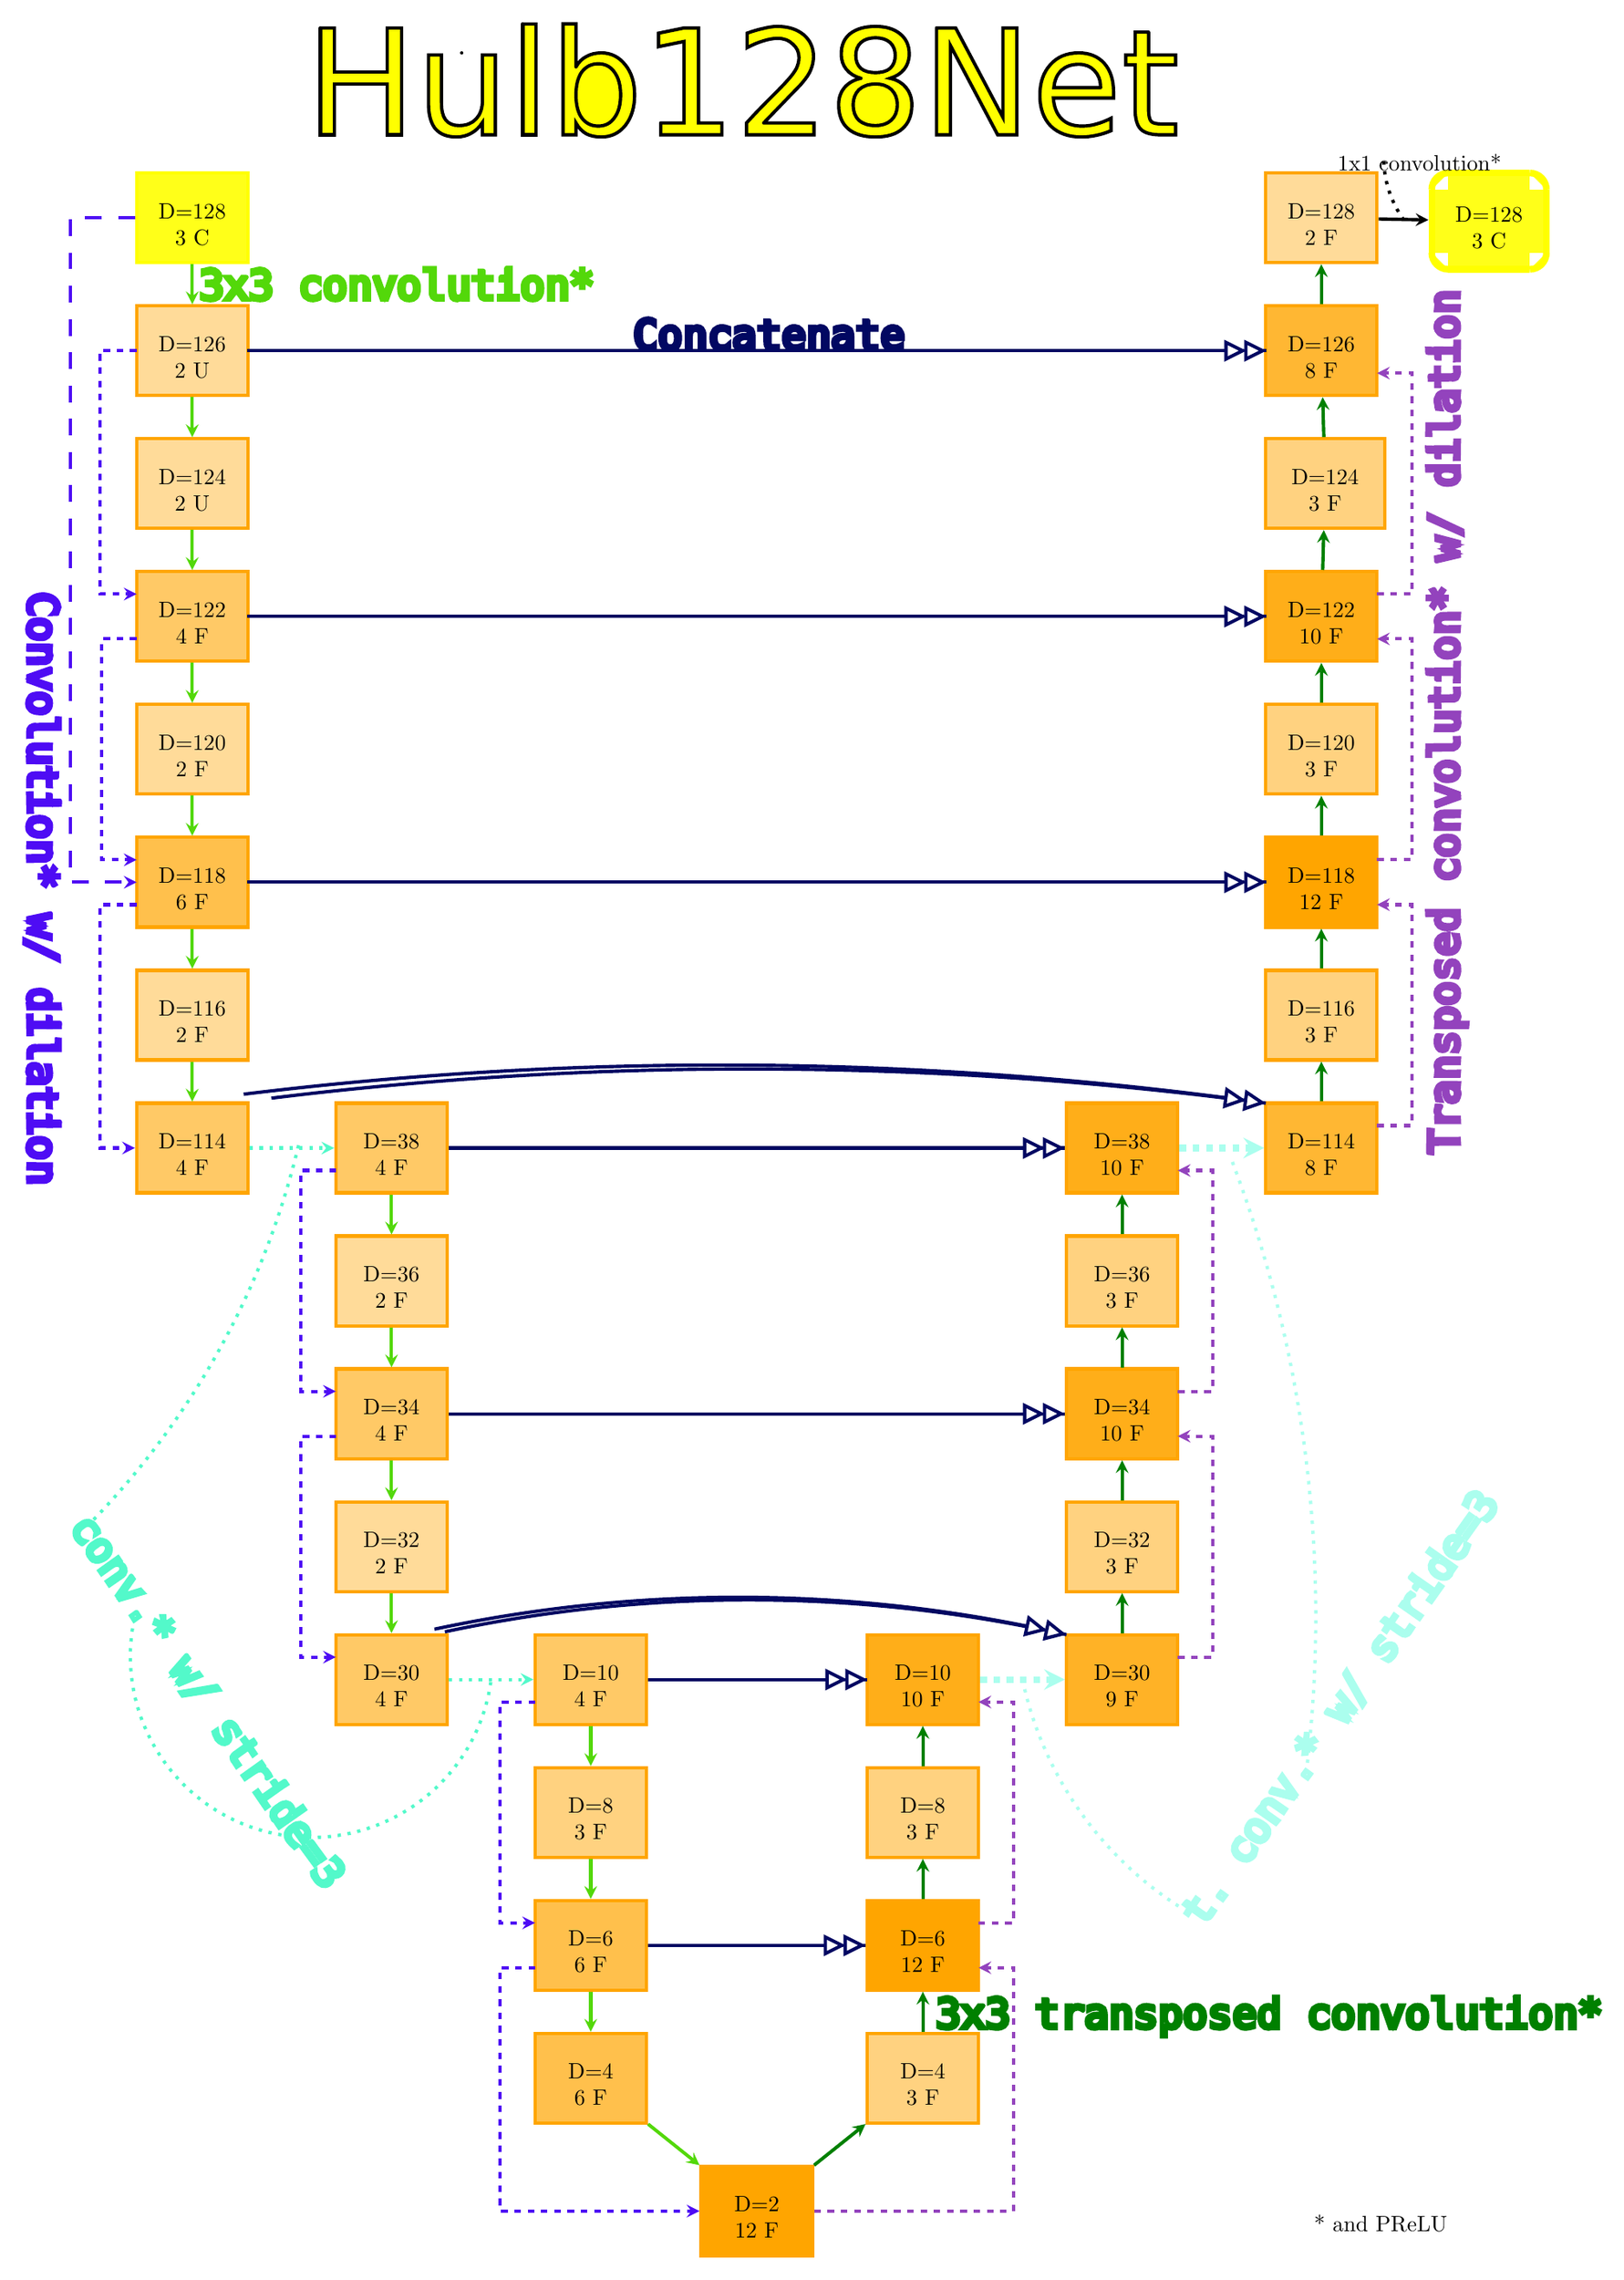
\begin{tikzpicture}
\pgftransformxscale{1.000000}
\pgftransformyscale{-1.000000}
\definecolor{dialinecolor}{rgb}{0.000000, 0.000000, 0.000000}
\pgfsetstrokecolor{dialinecolor}
\definecolor{dialinecolor}{rgb}{1.000000, 1.000000, 1.000000}
\pgfsetfillcolor{dialinecolor}
\definecolor{dialinecolor}{rgb}{1.000000, 1.000000, 0.098039}
\pgfsetfillcolor{dialinecolor}
\fill (22.000000\du,17.000000\du)--(22.000000\du,19.700000\du)--(25.352500\du,19.700000\du)--(25.352500\du,17.000000\du)--cycle;
\pgfsetlinewidth{0.100000\du}
\pgfsetdash{}{0pt}
\pgfsetdash{}{0pt}
\pgfsetmiterjoin
\definecolor{dialinecolor}{rgb}{1.000000, 1.000000, 0.000000}
\pgfsetstrokecolor{dialinecolor}
\draw (22.000000\du,17.000000\du)--(22.000000\du,19.700000\du)--(25.352500\du,19.700000\du)--(25.352500\du,17.000000\du)--cycle;
% setfont left to latex
\definecolor{dialinecolor}{rgb}{0.000000, 0.000000, 0.000000}
\pgfsetstrokecolor{dialinecolor}
\node at (23.676250\du,18.145000\du){D=128};
% setfont left to latex
\definecolor{dialinecolor}{rgb}{0.000000, 0.000000, 0.000000}
\pgfsetstrokecolor{dialinecolor}
\node at (23.676250\du,18.945000\du){3 C};
\definecolor{dialinecolor}{rgb}{1.000000, 0.858824, 0.600000}
\pgfsetfillcolor{dialinecolor}
\fill (22.000000\du,21.000000\du)--(22.000000\du,23.700000\du)--(25.352500\du,23.700000\du)--(25.352500\du,21.000000\du)--cycle;
\pgfsetlinewidth{0.100000\du}
\pgfsetdash{}{0pt}
\pgfsetdash{}{0pt}
\pgfsetmiterjoin
\definecolor{dialinecolor}{rgb}{1.000000, 0.647059, 0.000000}
\pgfsetstrokecolor{dialinecolor}
\draw (22.000000\du,21.000000\du)--(22.000000\du,23.700000\du)--(25.352500\du,23.700000\du)--(25.352500\du,21.000000\du)--cycle;
% setfont left to latex
\definecolor{dialinecolor}{rgb}{0.000000, 0.000000, 0.000000}
\pgfsetstrokecolor{dialinecolor}
\node at (23.676250\du,22.145000\du){D=126};
% setfont left to latex
\definecolor{dialinecolor}{rgb}{0.000000, 0.000000, 0.000000}
\pgfsetstrokecolor{dialinecolor}
\node at (23.676250\du,22.945000\du){2 U};
\definecolor{dialinecolor}{rgb}{1.000000, 0.858824, 0.600000}
\pgfsetfillcolor{dialinecolor}
\fill (22.000000\du,25.000000\du)--(22.000000\du,27.700000\du)--(25.352500\du,27.700000\du)--(25.352500\du,25.000000\du)--cycle;
\pgfsetlinewidth{0.100000\du}
\pgfsetdash{}{0pt}
\pgfsetdash{}{0pt}
\pgfsetmiterjoin
\definecolor{dialinecolor}{rgb}{1.000000, 0.647059, 0.000000}
\pgfsetstrokecolor{dialinecolor}
\draw (22.000000\du,25.000000\du)--(22.000000\du,27.700000\du)--(25.352500\du,27.700000\du)--(25.352500\du,25.000000\du)--cycle;
% setfont left to latex
\definecolor{dialinecolor}{rgb}{0.000000, 0.000000, 0.000000}
\pgfsetstrokecolor{dialinecolor}
\node at (23.676250\du,26.145000\du){D=124};
% setfont left to latex
\definecolor{dialinecolor}{rgb}{0.000000, 0.000000, 0.000000}
\pgfsetstrokecolor{dialinecolor}
\node at (23.676250\du,26.945000\du){2 U};
\definecolor{dialinecolor}{rgb}{1.000000, 0.788235, 0.400000}
\pgfsetfillcolor{dialinecolor}
\fill (22.000000\du,29.000000\du)--(22.000000\du,31.700000\du)--(25.352500\du,31.700000\du)--(25.352500\du,29.000000\du)--cycle;
\pgfsetlinewidth{0.100000\du}
\pgfsetdash{}{0pt}
\pgfsetdash{}{0pt}
\pgfsetmiterjoin
\definecolor{dialinecolor}{rgb}{1.000000, 0.647059, 0.000000}
\pgfsetstrokecolor{dialinecolor}
\draw (22.000000\du,29.000000\du)--(22.000000\du,31.700000\du)--(25.352500\du,31.700000\du)--(25.352500\du,29.000000\du)--cycle;
% setfont left to latex
\definecolor{dialinecolor}{rgb}{0.000000, 0.000000, 0.000000}
\pgfsetstrokecolor{dialinecolor}
\node at (23.676250\du,30.145000\du){D=122};
% setfont left to latex
\definecolor{dialinecolor}{rgb}{0.000000, 0.000000, 0.000000}
\pgfsetstrokecolor{dialinecolor}
\node at (23.676250\du,30.945000\du){ 4 F};
\definecolor{dialinecolor}{rgb}{1.000000, 0.858824, 0.600000}
\pgfsetfillcolor{dialinecolor}
\fill (22.000000\du,33.000000\du)--(22.000000\du,35.700000\du)--(25.352500\du,35.700000\du)--(25.352500\du,33.000000\du)--cycle;
\pgfsetlinewidth{0.100000\du}
\pgfsetdash{}{0pt}
\pgfsetdash{}{0pt}
\pgfsetmiterjoin
\definecolor{dialinecolor}{rgb}{1.000000, 0.647059, 0.000000}
\pgfsetstrokecolor{dialinecolor}
\draw (22.000000\du,33.000000\du)--(22.000000\du,35.700000\du)--(25.352500\du,35.700000\du)--(25.352500\du,33.000000\du)--cycle;
% setfont left to latex
\definecolor{dialinecolor}{rgb}{0.000000, 0.000000, 0.000000}
\pgfsetstrokecolor{dialinecolor}
\node at (23.676250\du,34.145000\du){D=120};
% setfont left to latex
\definecolor{dialinecolor}{rgb}{0.000000, 0.000000, 0.000000}
\pgfsetstrokecolor{dialinecolor}
\node at (23.676250\du,34.945000\du){ 2 F};
\pgfsetlinewidth{0.100000\du}
\pgfsetdash{}{0pt}
\pgfsetdash{}{0pt}
\pgfsetbuttcap
{
\definecolor{dialinecolor}{rgb}{0.325490, 0.847059, 0.039216}
\pgfsetfillcolor{dialinecolor}
% was here!!!
\pgfsetarrowsend{stealth}
\definecolor{dialinecolor}{rgb}{0.325490, 0.847059, 0.039216}
\pgfsetstrokecolor{dialinecolor}
\draw (23.676250\du,19.749414\du)--(23.676250\du,20.950586\du);
}
% setfont left to latex
\definecolor{dialinecolor}{rgb}{0.000000, 0.000000, 0.000000}
\pgfsetstrokecolor{dialinecolor}
\node[anchor=west] at (33.000000\du,23.000000\du){};
\pgfsetlinewidth{0.100000\du}
\pgfsetdash{}{0pt}
\pgfsetdash{}{0pt}
\pgfsetbuttcap
{
\definecolor{dialinecolor}{rgb}{0.325490, 0.847059, 0.039216}
\pgfsetfillcolor{dialinecolor}
% was here!!!
\pgfsetarrowsend{stealth}
\definecolor{dialinecolor}{rgb}{0.325490, 0.847059, 0.039216}
\pgfsetstrokecolor{dialinecolor}
\draw (23.676250\du,23.749414\du)--(23.676250\du,24.950586\du);
}
\pgfsetlinewidth{0.100000\du}
\pgfsetdash{}{0pt}
\pgfsetdash{}{0pt}
\pgfsetbuttcap
{
\definecolor{dialinecolor}{rgb}{0.325490, 0.847059, 0.039216}
\pgfsetfillcolor{dialinecolor}
% was here!!!
\pgfsetarrowsend{stealth}
\definecolor{dialinecolor}{rgb}{0.325490, 0.847059, 0.039216}
\pgfsetstrokecolor{dialinecolor}
\draw (23.676250\du,27.749414\du)--(23.676250\du,28.950586\du);
}
\definecolor{dialinecolor}{rgb}{1.000000, 0.752941, 0.298039}
\pgfsetfillcolor{dialinecolor}
\fill (22.000000\du,37.000000\du)--(22.000000\du,39.700000\du)--(25.352500\du,39.700000\du)--(25.352500\du,37.000000\du)--cycle;
\pgfsetlinewidth{0.100000\du}
\pgfsetdash{}{0pt}
\pgfsetdash{}{0pt}
\pgfsetmiterjoin
\definecolor{dialinecolor}{rgb}{1.000000, 0.647059, 0.000000}
\pgfsetstrokecolor{dialinecolor}
\draw (22.000000\du,37.000000\du)--(22.000000\du,39.700000\du)--(25.352500\du,39.700000\du)--(25.352500\du,37.000000\du)--cycle;
% setfont left to latex
\definecolor{dialinecolor}{rgb}{0.000000, 0.000000, 0.000000}
\pgfsetstrokecolor{dialinecolor}
\node at (23.676250\du,38.145000\du){D=118};
% setfont left to latex
\definecolor{dialinecolor}{rgb}{0.000000, 0.000000, 0.000000}
\pgfsetstrokecolor{dialinecolor}
\node at (23.676250\du,38.945000\du){6 F};
\pgfsetlinewidth{0.100000\du}
\pgfsetdash{}{0pt}
\pgfsetdash{}{0pt}
\pgfsetbuttcap
{
\definecolor{dialinecolor}{rgb}{0.325490, 0.847059, 0.039216}
\pgfsetfillcolor{dialinecolor}
% was here!!!
\pgfsetarrowsend{stealth}
\definecolor{dialinecolor}{rgb}{0.325490, 0.847059, 0.039216}
\pgfsetstrokecolor{dialinecolor}
\draw (23.676250\du,31.749414\du)--(23.676250\du,32.950586\du);
}
\pgfsetlinewidth{0.100000\du}
\pgfsetdash{}{0pt}
\pgfsetdash{}{0pt}
\pgfsetbuttcap
{
\definecolor{dialinecolor}{rgb}{0.325490, 0.847059, 0.039216}
\pgfsetfillcolor{dialinecolor}
% was here!!!
\pgfsetarrowsend{stealth}
\definecolor{dialinecolor}{rgb}{0.325490, 0.847059, 0.039216}
\pgfsetstrokecolor{dialinecolor}
\draw (23.676250\du,35.749414\du)--(23.676250\du,36.950586\du);
}
\pgfsetlinewidth{0.100000\du}
\pgfsetdash{{1.000000\du}{1.000000\du}}{0\du}
\pgfsetdash{{0.200000\du}{0.200000\du}}{0\du}
\pgfsetmiterjoin
\pgfsetbuttcap
{
\definecolor{dialinecolor}{rgb}{0.305882, 0.047059, 0.956863}
\pgfsetfillcolor{dialinecolor}
% was here!!!
\pgfsetarrowsend{stealth}
{\pgfsetcornersarced{\pgfpoint{0.000000\du}{0.000000\du}}\definecolor{dialinecolor}{rgb}{0.305882, 0.047059, 0.956863}
\pgfsetstrokecolor{dialinecolor}
\draw (22.000000\du,22.350000\du)--(20.899600\du,22.350000\du)--(20.899600\du,29.675000\du)--(22.000000\du,29.675000\du);
}}
\pgfsetlinewidth{0.100000\du}
\pgfsetdash{{0.200000\du}{0.200000\du}}{0\du}
\pgfsetdash{{0.200000\du}{0.200000\du}}{0\du}
\pgfsetmiterjoin
\pgfsetbuttcap
{
\definecolor{dialinecolor}{rgb}{0.305882, 0.047059, 0.956863}
\pgfsetfillcolor{dialinecolor}
% was here!!!
\pgfsetarrowsend{stealth}
{\pgfsetcornersarced{\pgfpoint{0.000000\du}{0.000000\du}}\definecolor{dialinecolor}{rgb}{0.305882, 0.047059, 0.956863}
\pgfsetstrokecolor{dialinecolor}
\draw (22.000000\du,31.025000\du)--(20.950000\du,31.025000\du)--(20.950000\du,37.675000\du)--(22.000000\du,37.675000\du);
}}
\definecolor{dialinecolor}{rgb}{1.000000, 0.858824, 0.600000}
\pgfsetfillcolor{dialinecolor}
\fill (22.000000\du,41.000000\du)--(22.000000\du,43.700000\du)--(25.352500\du,43.700000\du)--(25.352500\du,41.000000\du)--cycle;
\pgfsetlinewidth{0.100000\du}
\pgfsetdash{}{0pt}
\pgfsetdash{}{0pt}
\pgfsetmiterjoin
\definecolor{dialinecolor}{rgb}{1.000000, 0.647059, 0.000000}
\pgfsetstrokecolor{dialinecolor}
\draw (22.000000\du,41.000000\du)--(22.000000\du,43.700000\du)--(25.352500\du,43.700000\du)--(25.352500\du,41.000000\du)--cycle;
% setfont left to latex
\definecolor{dialinecolor}{rgb}{0.000000, 0.000000, 0.000000}
\pgfsetstrokecolor{dialinecolor}
\node at (23.676250\du,42.145000\du){D=116};
% setfont left to latex
\definecolor{dialinecolor}{rgb}{0.000000, 0.000000, 0.000000}
\pgfsetstrokecolor{dialinecolor}
\node at (23.676250\du,42.945000\du){ 2 F};
\definecolor{dialinecolor}{rgb}{1.000000, 0.788235, 0.400000}
\pgfsetfillcolor{dialinecolor}
\fill (22.000000\du,45.000000\du)--(22.000000\du,47.700000\du)--(25.352500\du,47.700000\du)--(25.352500\du,45.000000\du)--cycle;
\pgfsetlinewidth{0.100000\du}
\pgfsetdash{}{0pt}
\pgfsetdash{}{0pt}
\pgfsetmiterjoin
\definecolor{dialinecolor}{rgb}{1.000000, 0.647059, 0.000000}
\pgfsetstrokecolor{dialinecolor}
\draw (22.000000\du,45.000000\du)--(22.000000\du,47.700000\du)--(25.352500\du,47.700000\du)--(25.352500\du,45.000000\du)--cycle;
% setfont left to latex
\definecolor{dialinecolor}{rgb}{0.000000, 0.000000, 0.000000}
\pgfsetstrokecolor{dialinecolor}
\node at (23.676250\du,46.145000\du){D=114};
% setfont left to latex
\definecolor{dialinecolor}{rgb}{0.000000, 0.000000, 0.000000}
\pgfsetstrokecolor{dialinecolor}
\node at (23.676250\du,46.945000\du){ 4 F};
\definecolor{dialinecolor}{rgb}{1.000000, 0.788235, 0.400000}
\pgfsetfillcolor{dialinecolor}
\fill (28.000000\du,45.000000\du)--(28.000000\du,47.700000\du)--(31.352500\du,47.700000\du)--(31.352500\du,45.000000\du)--cycle;
\pgfsetlinewidth{0.100000\du}
\pgfsetdash{}{0pt}
\pgfsetdash{}{0pt}
\pgfsetmiterjoin
\definecolor{dialinecolor}{rgb}{1.000000, 0.647059, 0.000000}
\pgfsetstrokecolor{dialinecolor}
\draw (28.000000\du,45.000000\du)--(28.000000\du,47.700000\du)--(31.352500\du,47.700000\du)--(31.352500\du,45.000000\du)--cycle;
% setfont left to latex
\definecolor{dialinecolor}{rgb}{0.000000, 0.000000, 0.000000}
\pgfsetstrokecolor{dialinecolor}
\node at (29.676250\du,46.145000\du){D=38};
% setfont left to latex
\definecolor{dialinecolor}{rgb}{0.000000, 0.000000, 0.000000}
\pgfsetstrokecolor{dialinecolor}
\node at (29.676250\du,46.945000\du){4 F};
\definecolor{dialinecolor}{rgb}{1.000000, 0.858824, 0.600000}
\pgfsetfillcolor{dialinecolor}
\fill (28.000000\du,49.000000\du)--(28.000000\du,51.700000\du)--(31.352500\du,51.700000\du)--(31.352500\du,49.000000\du)--cycle;
\pgfsetlinewidth{0.100000\du}
\pgfsetdash{}{0pt}
\pgfsetdash{}{0pt}
\pgfsetmiterjoin
\definecolor{dialinecolor}{rgb}{1.000000, 0.647059, 0.000000}
\pgfsetstrokecolor{dialinecolor}
\draw (28.000000\du,49.000000\du)--(28.000000\du,51.700000\du)--(31.352500\du,51.700000\du)--(31.352500\du,49.000000\du)--cycle;
% setfont left to latex
\definecolor{dialinecolor}{rgb}{0.000000, 0.000000, 0.000000}
\pgfsetstrokecolor{dialinecolor}
\node at (29.676250\du,50.145000\du){D=36};
% setfont left to latex
\definecolor{dialinecolor}{rgb}{0.000000, 0.000000, 0.000000}
\pgfsetstrokecolor{dialinecolor}
\node at (29.676250\du,50.945000\du){ 2 F};
\definecolor{dialinecolor}{rgb}{1.000000, 0.788235, 0.400000}
\pgfsetfillcolor{dialinecolor}
\fill (28.000000\du,53.000000\du)--(28.000000\du,55.700000\du)--(31.352500\du,55.700000\du)--(31.352500\du,53.000000\du)--cycle;
\pgfsetlinewidth{0.100000\du}
\pgfsetdash{}{0pt}
\pgfsetdash{}{0pt}
\pgfsetmiterjoin
\definecolor{dialinecolor}{rgb}{1.000000, 0.647059, 0.000000}
\pgfsetstrokecolor{dialinecolor}
\draw (28.000000\du,53.000000\du)--(28.000000\du,55.700000\du)--(31.352500\du,55.700000\du)--(31.352500\du,53.000000\du)--cycle;
% setfont left to latex
\definecolor{dialinecolor}{rgb}{0.000000, 0.000000, 0.000000}
\pgfsetstrokecolor{dialinecolor}
\node at (29.676250\du,54.145000\du){D=34};
% setfont left to latex
\definecolor{dialinecolor}{rgb}{0.000000, 0.000000, 0.000000}
\pgfsetstrokecolor{dialinecolor}
\node at (29.676250\du,54.945000\du){4 F};
\definecolor{dialinecolor}{rgb}{1.000000, 0.788235, 0.400000}
\pgfsetfillcolor{dialinecolor}
\fill (34.000000\du,61.000000\du)--(34.000000\du,63.700000\du)--(37.352500\du,63.700000\du)--(37.352500\du,61.000000\du)--cycle;
\pgfsetlinewidth{0.100000\du}
\pgfsetdash{}{0pt}
\pgfsetdash{}{0pt}
\pgfsetmiterjoin
\definecolor{dialinecolor}{rgb}{1.000000, 0.647059, 0.000000}
\pgfsetstrokecolor{dialinecolor}
\draw (34.000000\du,61.000000\du)--(34.000000\du,63.700000\du)--(37.352500\du,63.700000\du)--(37.352500\du,61.000000\du)--cycle;
% setfont left to latex
\definecolor{dialinecolor}{rgb}{0.000000, 0.000000, 0.000000}
\pgfsetstrokecolor{dialinecolor}
\node at (35.676250\du,62.145000\du){D=10};
% setfont left to latex
\definecolor{dialinecolor}{rgb}{0.000000, 0.000000, 0.000000}
\pgfsetstrokecolor{dialinecolor}
\node at (35.676250\du,62.945000\du){4 F};
\definecolor{dialinecolor}{rgb}{1.000000, 0.823529, 0.501961}
\pgfsetfillcolor{dialinecolor}
\fill (34.000000\du,65.000000\du)--(34.000000\du,67.700000\du)--(37.352500\du,67.700000\du)--(37.352500\du,65.000000\du)--cycle;
\pgfsetlinewidth{0.100000\du}
\pgfsetdash{}{0pt}
\pgfsetdash{}{0pt}
\pgfsetmiterjoin
\definecolor{dialinecolor}{rgb}{1.000000, 0.647059, 0.000000}
\pgfsetstrokecolor{dialinecolor}
\draw (34.000000\du,65.000000\du)--(34.000000\du,67.700000\du)--(37.352500\du,67.700000\du)--(37.352500\du,65.000000\du)--cycle;
% setfont left to latex
\definecolor{dialinecolor}{rgb}{0.000000, 0.000000, 0.000000}
\pgfsetstrokecolor{dialinecolor}
\node at (35.676250\du,66.145000\du){D=8};
% setfont left to latex
\definecolor{dialinecolor}{rgb}{0.000000, 0.000000, 0.000000}
\pgfsetstrokecolor{dialinecolor}
\node at (35.676250\du,66.945000\du){3 F};
\definecolor{dialinecolor}{rgb}{1.000000, 0.752941, 0.298039}
\pgfsetfillcolor{dialinecolor}
\fill (34.000000\du,69.000000\du)--(34.000000\du,71.700000\du)--(37.352500\du,71.700000\du)--(37.352500\du,69.000000\du)--cycle;
\pgfsetlinewidth{0.100000\du}
\pgfsetdash{}{0pt}
\pgfsetdash{}{0pt}
\pgfsetmiterjoin
\definecolor{dialinecolor}{rgb}{1.000000, 0.647059, 0.000000}
\pgfsetstrokecolor{dialinecolor}
\draw (34.000000\du,69.000000\du)--(34.000000\du,71.700000\du)--(37.352500\du,71.700000\du)--(37.352500\du,69.000000\du)--cycle;
% setfont left to latex
\definecolor{dialinecolor}{rgb}{0.000000, 0.000000, 0.000000}
\pgfsetstrokecolor{dialinecolor}
\node at (35.676250\du,70.145000\du){D=6};
% setfont left to latex
\definecolor{dialinecolor}{rgb}{0.000000, 0.000000, 0.000000}
\pgfsetstrokecolor{dialinecolor}
\node at (35.676250\du,70.945000\du){6 F};
\definecolor{dialinecolor}{rgb}{1.000000, 0.752941, 0.298039}
\pgfsetfillcolor{dialinecolor}
\fill (34.000000\du,73.000000\du)--(34.000000\du,75.700000\du)--(37.352500\du,75.700000\du)--(37.352500\du,73.000000\du)--cycle;
\pgfsetlinewidth{0.100000\du}
\pgfsetdash{}{0pt}
\pgfsetdash{}{0pt}
\pgfsetmiterjoin
\definecolor{dialinecolor}{rgb}{1.000000, 0.647059, 0.000000}
\pgfsetstrokecolor{dialinecolor}
\draw (34.000000\du,73.000000\du)--(34.000000\du,75.700000\du)--(37.352500\du,75.700000\du)--(37.352500\du,73.000000\du)--cycle;
% setfont left to latex
\definecolor{dialinecolor}{rgb}{0.000000, 0.000000, 0.000000}
\pgfsetstrokecolor{dialinecolor}
\node at (35.676250\du,74.145000\du){D=4};
% setfont left to latex
\definecolor{dialinecolor}{rgb}{0.000000, 0.000000, 0.000000}
\pgfsetstrokecolor{dialinecolor}
\node at (35.676250\du,74.945000\du){6 F};
\definecolor{dialinecolor}{rgb}{1.000000, 0.647059, 0.000000}
\pgfsetfillcolor{dialinecolor}
\fill (39.000000\du,77.000000\du)--(39.000000\du,79.700000\du)--(42.352500\du,79.700000\du)--(42.352500\du,77.000000\du)--cycle;
\pgfsetlinewidth{0.100000\du}
\pgfsetdash{}{0pt}
\pgfsetdash{}{0pt}
\pgfsetmiterjoin
\definecolor{dialinecolor}{rgb}{1.000000, 0.647059, 0.000000}
\pgfsetstrokecolor{dialinecolor}
\draw (39.000000\du,77.000000\du)--(39.000000\du,79.700000\du)--(42.352500\du,79.700000\du)--(42.352500\du,77.000000\du)--cycle;
% setfont left to latex
\definecolor{dialinecolor}{rgb}{0.000000, 0.000000, 0.000000}
\pgfsetstrokecolor{dialinecolor}
\node at (40.676250\du,78.145000\du){D=2};
% setfont left to latex
\definecolor{dialinecolor}{rgb}{0.000000, 0.000000, 0.000000}
\pgfsetstrokecolor{dialinecolor}
\node at (40.676250\du,78.945000\du){12 F};
\definecolor{dialinecolor}{rgb}{1.000000, 0.858824, 0.600000}
\pgfsetfillcolor{dialinecolor}
\fill (28.000000\du,57.000000\du)--(28.000000\du,59.700000\du)--(31.352500\du,59.700000\du)--(31.352500\du,57.000000\du)--cycle;
\pgfsetlinewidth{0.100000\du}
\pgfsetdash{}{0pt}
\pgfsetdash{}{0pt}
\pgfsetmiterjoin
\definecolor{dialinecolor}{rgb}{1.000000, 0.647059, 0.000000}
\pgfsetstrokecolor{dialinecolor}
\draw (28.000000\du,57.000000\du)--(28.000000\du,59.700000\du)--(31.352500\du,59.700000\du)--(31.352500\du,57.000000\du)--cycle;
% setfont left to latex
\definecolor{dialinecolor}{rgb}{0.000000, 0.000000, 0.000000}
\pgfsetstrokecolor{dialinecolor}
\node at (29.676250\du,58.145000\du){D=32};
% setfont left to latex
\definecolor{dialinecolor}{rgb}{0.000000, 0.000000, 0.000000}
\pgfsetstrokecolor{dialinecolor}
\node at (29.676250\du,58.945000\du){ 2 F};
\definecolor{dialinecolor}{rgb}{1.000000, 0.788235, 0.400000}
\pgfsetfillcolor{dialinecolor}
\fill (28.000000\du,61.000000\du)--(28.000000\du,63.700000\du)--(31.352500\du,63.700000\du)--(31.352500\du,61.000000\du)--cycle;
\pgfsetlinewidth{0.100000\du}
\pgfsetdash{}{0pt}
\pgfsetdash{}{0pt}
\pgfsetmiterjoin
\definecolor{dialinecolor}{rgb}{1.000000, 0.647059, 0.000000}
\pgfsetstrokecolor{dialinecolor}
\draw (28.000000\du,61.000000\du)--(28.000000\du,63.700000\du)--(31.352500\du,63.700000\du)--(31.352500\du,61.000000\du)--cycle;
% setfont left to latex
\definecolor{dialinecolor}{rgb}{0.000000, 0.000000, 0.000000}
\pgfsetstrokecolor{dialinecolor}
\node at (29.676250\du,62.145000\du){D=30};
% setfont left to latex
\definecolor{dialinecolor}{rgb}{0.000000, 0.000000, 0.000000}
\pgfsetstrokecolor{dialinecolor}
\node at (29.676250\du,62.945000\du){ 4 F};
\definecolor{dialinecolor}{rgb}{1.000000, 0.858824, 0.600000}
\pgfsetfillcolor{dialinecolor}
\fill (56.000000\du,17.000000\du)--(56.000000\du,19.700000\du)--(59.352500\du,19.700000\du)--(59.352500\du,17.000000\du)--cycle;
\pgfsetlinewidth{0.100000\du}
\pgfsetdash{}{0pt}
\pgfsetdash{}{0pt}
\pgfsetmiterjoin
\definecolor{dialinecolor}{rgb}{1.000000, 0.647059, 0.000000}
\pgfsetstrokecolor{dialinecolor}
\draw (56.000000\du,17.000000\du)--(56.000000\du,19.700000\du)--(59.352500\du,19.700000\du)--(59.352500\du,17.000000\du)--cycle;
% setfont left to latex
\definecolor{dialinecolor}{rgb}{0.000000, 0.000000, 0.000000}
\pgfsetstrokecolor{dialinecolor}
\node at (57.676250\du,18.145000\du){D=128};
% setfont left to latex
\definecolor{dialinecolor}{rgb}{0.000000, 0.000000, 0.000000}
\pgfsetstrokecolor{dialinecolor}
\node at (57.676250\du,18.945000\du){2 F};
\definecolor{dialinecolor}{rgb}{1.000000, 0.717647, 0.200000}
\pgfsetfillcolor{dialinecolor}
\fill (56.000000\du,21.000000\du)--(56.000000\du,23.700000\du)--(59.352500\du,23.700000\du)--(59.352500\du,21.000000\du)--cycle;
\pgfsetlinewidth{0.100000\du}
\pgfsetdash{}{0pt}
\pgfsetdash{}{0pt}
\pgfsetmiterjoin
\definecolor{dialinecolor}{rgb}{1.000000, 0.647059, 0.000000}
\pgfsetstrokecolor{dialinecolor}
\draw (56.000000\du,21.000000\du)--(56.000000\du,23.700000\du)--(59.352500\du,23.700000\du)--(59.352500\du,21.000000\du)--cycle;
% setfont left to latex
\definecolor{dialinecolor}{rgb}{0.000000, 0.000000, 0.000000}
\pgfsetstrokecolor{dialinecolor}
\node at (57.676250\du,22.145000\du){D=126};
% setfont left to latex
\definecolor{dialinecolor}{rgb}{0.000000, 0.000000, 0.000000}
\pgfsetstrokecolor{dialinecolor}
\node at (57.676250\du,22.945000\du){8 F};
\definecolor{dialinecolor}{rgb}{1.000000, 0.823529, 0.501961}
\pgfsetfillcolor{dialinecolor}
\fill (56.000000\du,25.000000\du)--(56.000000\du,27.700000\du)--(59.578750\du,27.700000\du)--(59.578750\du,25.000000\du)--cycle;
\pgfsetlinewidth{0.100000\du}
\pgfsetdash{}{0pt}
\pgfsetdash{}{0pt}
\pgfsetmiterjoin
\definecolor{dialinecolor}{rgb}{1.000000, 0.647059, 0.000000}
\pgfsetstrokecolor{dialinecolor}
\draw (56.000000\du,25.000000\du)--(56.000000\du,27.700000\du)--(59.578750\du,27.700000\du)--(59.578750\du,25.000000\du)--cycle;
% setfont left to latex
\definecolor{dialinecolor}{rgb}{0.000000, 0.000000, 0.000000}
\pgfsetstrokecolor{dialinecolor}
\node at (57.789375\du,26.145000\du){D=124};
% setfont left to latex
\definecolor{dialinecolor}{rgb}{0.000000, 0.000000, 0.000000}
\pgfsetstrokecolor{dialinecolor}
\node at (57.789375\du,26.945000\du){3 F};
\definecolor{dialinecolor}{rgb}{1.000000, 0.682353, 0.098039}
\pgfsetfillcolor{dialinecolor}
\fill (56.000000\du,29.000000\du)--(56.000000\du,31.700000\du)--(59.352500\du,31.700000\du)--(59.352500\du,29.000000\du)--cycle;
\pgfsetlinewidth{0.100000\du}
\pgfsetdash{}{0pt}
\pgfsetdash{}{0pt}
\pgfsetmiterjoin
\definecolor{dialinecolor}{rgb}{1.000000, 0.647059, 0.000000}
\pgfsetstrokecolor{dialinecolor}
\draw (56.000000\du,29.000000\du)--(56.000000\du,31.700000\du)--(59.352500\du,31.700000\du)--(59.352500\du,29.000000\du)--cycle;
% setfont left to latex
\definecolor{dialinecolor}{rgb}{0.000000, 0.000000, 0.000000}
\pgfsetstrokecolor{dialinecolor}
\node at (57.676250\du,30.145000\du){D=122};
% setfont left to latex
\definecolor{dialinecolor}{rgb}{0.000000, 0.000000, 0.000000}
\pgfsetstrokecolor{dialinecolor}
\node at (57.676250\du,30.945000\du){10 F};
\definecolor{dialinecolor}{rgb}{1.000000, 0.823529, 0.501961}
\pgfsetfillcolor{dialinecolor}
\fill (56.000000\du,33.000000\du)--(56.000000\du,35.700000\du)--(59.352500\du,35.700000\du)--(59.352500\du,33.000000\du)--cycle;
\pgfsetlinewidth{0.100000\du}
\pgfsetdash{}{0pt}
\pgfsetdash{}{0pt}
\pgfsetmiterjoin
\definecolor{dialinecolor}{rgb}{1.000000, 0.647059, 0.000000}
\pgfsetstrokecolor{dialinecolor}
\draw (56.000000\du,33.000000\du)--(56.000000\du,35.700000\du)--(59.352500\du,35.700000\du)--(59.352500\du,33.000000\du)--cycle;
% setfont left to latex
\definecolor{dialinecolor}{rgb}{0.000000, 0.000000, 0.000000}
\pgfsetstrokecolor{dialinecolor}
\node at (57.676250\du,34.145000\du){D=120};
% setfont left to latex
\definecolor{dialinecolor}{rgb}{0.000000, 0.000000, 0.000000}
\pgfsetstrokecolor{dialinecolor}
\node at (57.676250\du,34.945000\du){3 F};
% setfont left to latex
\definecolor{dialinecolor}{rgb}{0.000000, 0.000000, 0.000000}
\pgfsetstrokecolor{dialinecolor}
\node[anchor=west] at (64.000000\du,22.000000\du){};
\definecolor{dialinecolor}{rgb}{1.000000, 0.647059, 0.000000}
\pgfsetfillcolor{dialinecolor}
\fill (56.000000\du,37.000000\du)--(56.000000\du,39.700000\du)--(59.352500\du,39.700000\du)--(59.352500\du,37.000000\du)--cycle;
\pgfsetlinewidth{0.100000\du}
\pgfsetdash{}{0pt}
\pgfsetdash{}{0pt}
\pgfsetmiterjoin
\definecolor{dialinecolor}{rgb}{1.000000, 0.647059, 0.000000}
\pgfsetstrokecolor{dialinecolor}
\draw (56.000000\du,37.000000\du)--(56.000000\du,39.700000\du)--(59.352500\du,39.700000\du)--(59.352500\du,37.000000\du)--cycle;
% setfont left to latex
\definecolor{dialinecolor}{rgb}{0.000000, 0.000000, 0.000000}
\pgfsetstrokecolor{dialinecolor}
\node at (57.676250\du,38.145000\du){D=118};
% setfont left to latex
\definecolor{dialinecolor}{rgb}{0.000000, 0.000000, 0.000000}
\pgfsetstrokecolor{dialinecolor}
\node at (57.676250\du,38.945000\du){12 F};
\definecolor{dialinecolor}{rgb}{1.000000, 0.823529, 0.501961}
\pgfsetfillcolor{dialinecolor}
\fill (56.000000\du,41.000000\du)--(56.000000\du,43.700000\du)--(59.352500\du,43.700000\du)--(59.352500\du,41.000000\du)--cycle;
\pgfsetlinewidth{0.100000\du}
\pgfsetdash{}{0pt}
\pgfsetdash{}{0pt}
\pgfsetmiterjoin
\definecolor{dialinecolor}{rgb}{1.000000, 0.647059, 0.000000}
\pgfsetstrokecolor{dialinecolor}
\draw (56.000000\du,41.000000\du)--(56.000000\du,43.700000\du)--(59.352500\du,43.700000\du)--(59.352500\du,41.000000\du)--cycle;
% setfont left to latex
\definecolor{dialinecolor}{rgb}{0.000000, 0.000000, 0.000000}
\pgfsetstrokecolor{dialinecolor}
\node at (57.676250\du,42.145000\du){D=116};
% setfont left to latex
\definecolor{dialinecolor}{rgb}{0.000000, 0.000000, 0.000000}
\pgfsetstrokecolor{dialinecolor}
\node at (57.676250\du,42.945000\du){3 F};
\definecolor{dialinecolor}{rgb}{1.000000, 0.717647, 0.200000}
\pgfsetfillcolor{dialinecolor}
\fill (56.000000\du,45.000000\du)--(56.000000\du,47.700000\du)--(59.352500\du,47.700000\du)--(59.352500\du,45.000000\du)--cycle;
\pgfsetlinewidth{0.100000\du}
\pgfsetdash{}{0pt}
\pgfsetdash{}{0pt}
\pgfsetmiterjoin
\definecolor{dialinecolor}{rgb}{1.000000, 0.647059, 0.000000}
\pgfsetstrokecolor{dialinecolor}
\draw (56.000000\du,45.000000\du)--(56.000000\du,47.700000\du)--(59.352500\du,47.700000\du)--(59.352500\du,45.000000\du)--cycle;
% setfont left to latex
\definecolor{dialinecolor}{rgb}{0.000000, 0.000000, 0.000000}
\pgfsetstrokecolor{dialinecolor}
\node at (57.676250\du,46.145000\du){D=114};
% setfont left to latex
\definecolor{dialinecolor}{rgb}{0.000000, 0.000000, 0.000000}
\pgfsetstrokecolor{dialinecolor}
\node at (57.676250\du,46.945000\du){8 F};
\definecolor{dialinecolor}{rgb}{1.000000, 0.682353, 0.098039}
\pgfsetfillcolor{dialinecolor}
\fill (50.000000\du,45.000000\du)--(50.000000\du,47.700000\du)--(53.352500\du,47.700000\du)--(53.352500\du,45.000000\du)--cycle;
\pgfsetlinewidth{0.100000\du}
\pgfsetdash{}{0pt}
\pgfsetdash{}{0pt}
\pgfsetmiterjoin
\definecolor{dialinecolor}{rgb}{1.000000, 0.647059, 0.000000}
\pgfsetstrokecolor{dialinecolor}
\draw (50.000000\du,45.000000\du)--(50.000000\du,47.700000\du)--(53.352500\du,47.700000\du)--(53.352500\du,45.000000\du)--cycle;
% setfont left to latex
\definecolor{dialinecolor}{rgb}{0.000000, 0.000000, 0.000000}
\pgfsetstrokecolor{dialinecolor}
\node at (51.676250\du,46.145000\du){D=38};
% setfont left to latex
\definecolor{dialinecolor}{rgb}{0.000000, 0.000000, 0.000000}
\pgfsetstrokecolor{dialinecolor}
\node at (51.676250\du,46.945000\du){10 F};
\definecolor{dialinecolor}{rgb}{1.000000, 0.823529, 0.501961}
\pgfsetfillcolor{dialinecolor}
\fill (50.000000\du,49.000000\du)--(50.000000\du,51.700000\du)--(53.352500\du,51.700000\du)--(53.352500\du,49.000000\du)--cycle;
\pgfsetlinewidth{0.100000\du}
\pgfsetdash{}{0pt}
\pgfsetdash{}{0pt}
\pgfsetmiterjoin
\definecolor{dialinecolor}{rgb}{1.000000, 0.647059, 0.000000}
\pgfsetstrokecolor{dialinecolor}
\draw (50.000000\du,49.000000\du)--(50.000000\du,51.700000\du)--(53.352500\du,51.700000\du)--(53.352500\du,49.000000\du)--cycle;
% setfont left to latex
\definecolor{dialinecolor}{rgb}{0.000000, 0.000000, 0.000000}
\pgfsetstrokecolor{dialinecolor}
\node at (51.676250\du,50.145000\du){D=36};
% setfont left to latex
\definecolor{dialinecolor}{rgb}{0.000000, 0.000000, 0.000000}
\pgfsetstrokecolor{dialinecolor}
\node at (51.676250\du,50.945000\du){3 F};
\definecolor{dialinecolor}{rgb}{1.000000, 0.682353, 0.098039}
\pgfsetfillcolor{dialinecolor}
\fill (50.000000\du,53.000000\du)--(50.000000\du,55.700000\du)--(53.352500\du,55.700000\du)--(53.352500\du,53.000000\du)--cycle;
\pgfsetlinewidth{0.100000\du}
\pgfsetdash{}{0pt}
\pgfsetdash{}{0pt}
\pgfsetmiterjoin
\definecolor{dialinecolor}{rgb}{1.000000, 0.647059, 0.000000}
\pgfsetstrokecolor{dialinecolor}
\draw (50.000000\du,53.000000\du)--(50.000000\du,55.700000\du)--(53.352500\du,55.700000\du)--(53.352500\du,53.000000\du)--cycle;
% setfont left to latex
\definecolor{dialinecolor}{rgb}{0.000000, 0.000000, 0.000000}
\pgfsetstrokecolor{dialinecolor}
\node at (51.676250\du,54.145000\du){D=34};
% setfont left to latex
\definecolor{dialinecolor}{rgb}{0.000000, 0.000000, 0.000000}
\pgfsetstrokecolor{dialinecolor}
\node at (51.676250\du,54.945000\du){10 F};
\definecolor{dialinecolor}{rgb}{1.000000, 0.682353, 0.098039}
\pgfsetfillcolor{dialinecolor}
\fill (44.000000\du,61.000000\du)--(44.000000\du,63.700000\du)--(47.352500\du,63.700000\du)--(47.352500\du,61.000000\du)--cycle;
\pgfsetlinewidth{0.100000\du}
\pgfsetdash{}{0pt}
\pgfsetdash{}{0pt}
\pgfsetmiterjoin
\definecolor{dialinecolor}{rgb}{1.000000, 0.647059, 0.000000}
\pgfsetstrokecolor{dialinecolor}
\draw (44.000000\du,61.000000\du)--(44.000000\du,63.700000\du)--(47.352500\du,63.700000\du)--(47.352500\du,61.000000\du)--cycle;
% setfont left to latex
\definecolor{dialinecolor}{rgb}{0.000000, 0.000000, 0.000000}
\pgfsetstrokecolor{dialinecolor}
\node at (45.676250\du,62.145000\du){D=10};
% setfont left to latex
\definecolor{dialinecolor}{rgb}{0.000000, 0.000000, 0.000000}
\pgfsetstrokecolor{dialinecolor}
\node at (45.676250\du,62.945000\du){10 F};
\definecolor{dialinecolor}{rgb}{1.000000, 0.823529, 0.501961}
\pgfsetfillcolor{dialinecolor}
\fill (44.000000\du,65.000000\du)--(44.000000\du,67.700000\du)--(47.352500\du,67.700000\du)--(47.352500\du,65.000000\du)--cycle;
\pgfsetlinewidth{0.100000\du}
\pgfsetdash{}{0pt}
\pgfsetdash{}{0pt}
\pgfsetmiterjoin
\definecolor{dialinecolor}{rgb}{1.000000, 0.647059, 0.000000}
\pgfsetstrokecolor{dialinecolor}
\draw (44.000000\du,65.000000\du)--(44.000000\du,67.700000\du)--(47.352500\du,67.700000\du)--(47.352500\du,65.000000\du)--cycle;
% setfont left to latex
\definecolor{dialinecolor}{rgb}{0.000000, 0.000000, 0.000000}
\pgfsetstrokecolor{dialinecolor}
\node at (45.676250\du,66.145000\du){D=8};
% setfont left to latex
\definecolor{dialinecolor}{rgb}{0.000000, 0.000000, 0.000000}
\pgfsetstrokecolor{dialinecolor}
\node at (45.676250\du,66.945000\du){3 F};
\definecolor{dialinecolor}{rgb}{1.000000, 0.647059, 0.000000}
\pgfsetfillcolor{dialinecolor}
\fill (44.000000\du,69.000000\du)--(44.000000\du,71.700000\du)--(47.352500\du,71.700000\du)--(47.352500\du,69.000000\du)--cycle;
\pgfsetlinewidth{0.100000\du}
\pgfsetdash{}{0pt}
\pgfsetdash{}{0pt}
\pgfsetmiterjoin
\definecolor{dialinecolor}{rgb}{1.000000, 0.647059, 0.000000}
\pgfsetstrokecolor{dialinecolor}
\draw (44.000000\du,69.000000\du)--(44.000000\du,71.700000\du)--(47.352500\du,71.700000\du)--(47.352500\du,69.000000\du)--cycle;
% setfont left to latex
\definecolor{dialinecolor}{rgb}{0.000000, 0.000000, 0.000000}
\pgfsetstrokecolor{dialinecolor}
\node at (45.676250\du,70.145000\du){D=6};
% setfont left to latex
\definecolor{dialinecolor}{rgb}{0.000000, 0.000000, 0.000000}
\pgfsetstrokecolor{dialinecolor}
\node at (45.676250\du,70.945000\du){12 F};
\definecolor{dialinecolor}{rgb}{1.000000, 0.823529, 0.501961}
\pgfsetfillcolor{dialinecolor}
\fill (44.000000\du,73.000000\du)--(44.000000\du,75.700000\du)--(47.352500\du,75.700000\du)--(47.352500\du,73.000000\du)--cycle;
\pgfsetlinewidth{0.100000\du}
\pgfsetdash{}{0pt}
\pgfsetdash{}{0pt}
\pgfsetmiterjoin
\definecolor{dialinecolor}{rgb}{1.000000, 0.647059, 0.000000}
\pgfsetstrokecolor{dialinecolor}
\draw (44.000000\du,73.000000\du)--(44.000000\du,75.700000\du)--(47.352500\du,75.700000\du)--(47.352500\du,73.000000\du)--cycle;
% setfont left to latex
\definecolor{dialinecolor}{rgb}{0.000000, 0.000000, 0.000000}
\pgfsetstrokecolor{dialinecolor}
\node at (45.676250\du,74.145000\du){D=4};
% setfont left to latex
\definecolor{dialinecolor}{rgb}{0.000000, 0.000000, 0.000000}
\pgfsetstrokecolor{dialinecolor}
\node at (45.676250\du,74.945000\du){3 F};
\definecolor{dialinecolor}{rgb}{1.000000, 0.823529, 0.501961}
\pgfsetfillcolor{dialinecolor}
\fill (50.000000\du,57.000000\du)--(50.000000\du,59.700000\du)--(53.352500\du,59.700000\du)--(53.352500\du,57.000000\du)--cycle;
\pgfsetlinewidth{0.100000\du}
\pgfsetdash{}{0pt}
\pgfsetdash{}{0pt}
\pgfsetmiterjoin
\definecolor{dialinecolor}{rgb}{1.000000, 0.647059, 0.000000}
\pgfsetstrokecolor{dialinecolor}
\draw (50.000000\du,57.000000\du)--(50.000000\du,59.700000\du)--(53.352500\du,59.700000\du)--(53.352500\du,57.000000\du)--cycle;
% setfont left to latex
\definecolor{dialinecolor}{rgb}{0.000000, 0.000000, 0.000000}
\pgfsetstrokecolor{dialinecolor}
\node at (51.676250\du,58.145000\du){D=32};
% setfont left to latex
\definecolor{dialinecolor}{rgb}{0.000000, 0.000000, 0.000000}
\pgfsetstrokecolor{dialinecolor}
\node at (51.676250\du,58.945000\du){3 F};
\definecolor{dialinecolor}{rgb}{1.000000, 0.698039, 0.149020}
\pgfsetfillcolor{dialinecolor}
\fill (50.000000\du,61.000000\du)--(50.000000\du,63.700000\du)--(53.352500\du,63.700000\du)--(53.352500\du,61.000000\du)--cycle;
\pgfsetlinewidth{0.100000\du}
\pgfsetdash{}{0pt}
\pgfsetdash{}{0pt}
\pgfsetmiterjoin
\definecolor{dialinecolor}{rgb}{1.000000, 0.647059, 0.000000}
\pgfsetstrokecolor{dialinecolor}
\draw (50.000000\du,61.000000\du)--(50.000000\du,63.700000\du)--(53.352500\du,63.700000\du)--(53.352500\du,61.000000\du)--cycle;
% setfont left to latex
\definecolor{dialinecolor}{rgb}{0.000000, 0.000000, 0.000000}
\pgfsetstrokecolor{dialinecolor}
\node at (51.676250\du,62.145000\du){D=30};
% setfont left to latex
\definecolor{dialinecolor}{rgb}{0.000000, 0.000000, 0.000000}
\pgfsetstrokecolor{dialinecolor}
\node at (51.676250\du,62.945000\du){9 F};
\pgfsetlinewidth{0.100000\du}
\pgfsetdash{{1.000000\du}{1.000000\du}}{0\du}
\pgfsetdash{{0.200000\du}{0.200000\du}}{0\du}
\pgfsetmiterjoin
\pgfsetbuttcap
{
\definecolor{dialinecolor}{rgb}{0.305882, 0.047059, 0.956863}
\pgfsetfillcolor{dialinecolor}
% was here!!!
\pgfsetarrowsend{stealth}
{\pgfsetcornersarced{\pgfpoint{0.000000\du}{0.000000\du}}\definecolor{dialinecolor}{rgb}{0.305882, 0.047059, 0.956863}
\pgfsetstrokecolor{dialinecolor}
\draw (22.000000\du,39.025000\du)--(20.899579\du,39.025000\du)--(20.899579\du,46.350000\du)--(21.949579\du,46.350000\du);
}}
\pgfsetlinewidth{0.100000\du}
\pgfsetdash{}{0pt}
\pgfsetdash{}{0pt}
\pgfsetbuttcap
{
\definecolor{dialinecolor}{rgb}{0.325490, 0.847059, 0.039216}
\pgfsetfillcolor{dialinecolor}
% was here!!!
\pgfsetarrowsend{stealth}
\definecolor{dialinecolor}{rgb}{0.325490, 0.847059, 0.039216}
\pgfsetstrokecolor{dialinecolor}
\draw (23.676250\du,39.749414\du)--(23.676250\du,40.950586\du);
}
\pgfsetlinewidth{0.100000\du}
\pgfsetdash{}{0pt}
\pgfsetdash{}{0pt}
\pgfsetbuttcap
{
\definecolor{dialinecolor}{rgb}{0.325490, 0.847059, 0.039216}
\pgfsetfillcolor{dialinecolor}
% was here!!!
\pgfsetarrowsend{stealth}
\definecolor{dialinecolor}{rgb}{0.325490, 0.847059, 0.039216}
\pgfsetstrokecolor{dialinecolor}
\draw (23.676250\du,43.749414\du)--(23.676250\du,44.950586\du);
}
\pgfsetlinewidth{0.100000\du}
\pgfsetdash{{\pgflinewidth}{0.200000\du}}{0cm}
\pgfsetdash{{\pgflinewidth}{0.200000\du}}{0cm}
\pgfsetbuttcap
{
\definecolor{dialinecolor}{rgb}{0.325490, 0.976471, 0.792157}
\pgfsetfillcolor{dialinecolor}
% was here!!!
\pgfsetarrowsend{stealth}
\definecolor{dialinecolor}{rgb}{0.325490, 0.976471, 0.792157}
\pgfsetstrokecolor{dialinecolor}
\draw (25.402568\du,46.350000\du)--(27.949932\du,46.350000\du);
}
\pgfsetlinewidth{0.100000\du}
\pgfsetdash{}{0pt}
\pgfsetdash{}{0pt}
\pgfsetbuttcap
{
\definecolor{dialinecolor}{rgb}{0.325490, 0.847059, 0.039216}
\pgfsetfillcolor{dialinecolor}
% was here!!!
\pgfsetarrowsend{stealth}
\definecolor{dialinecolor}{rgb}{0.325490, 0.847059, 0.039216}
\pgfsetstrokecolor{dialinecolor}
\draw (29.676250\du,47.749414\du)--(29.676250\du,48.950586\du);
}
\pgfsetlinewidth{0.100000\du}
\pgfsetdash{}{0pt}
\pgfsetdash{}{0pt}
\pgfsetbuttcap
{
\definecolor{dialinecolor}{rgb}{0.325490, 0.847059, 0.039216}
\pgfsetfillcolor{dialinecolor}
% was here!!!
\pgfsetarrowsend{stealth}
\definecolor{dialinecolor}{rgb}{0.325490, 0.847059, 0.039216}
\pgfsetstrokecolor{dialinecolor}
\draw (29.676250\du,51.749414\du)--(29.676250\du,52.950586\du);
}
\pgfsetlinewidth{0.100000\du}
\pgfsetdash{}{0pt}
\pgfsetdash{}{0pt}
\pgfsetbuttcap
{
\definecolor{dialinecolor}{rgb}{0.325490, 0.847059, 0.039216}
\pgfsetfillcolor{dialinecolor}
% was here!!!
\pgfsetarrowsend{stealth}
\definecolor{dialinecolor}{rgb}{0.325490, 0.847059, 0.039216}
\pgfsetstrokecolor{dialinecolor}
\draw (29.676250\du,55.749414\du)--(29.676250\du,56.950586\du);
}
\pgfsetlinewidth{0.100000\du}
\pgfsetdash{}{0pt}
\pgfsetdash{}{0pt}
\pgfsetbuttcap
{
\definecolor{dialinecolor}{rgb}{0.325490, 0.847059, 0.039216}
\pgfsetfillcolor{dialinecolor}
% was here!!!
\pgfsetarrowsend{stealth}
\definecolor{dialinecolor}{rgb}{0.325490, 0.847059, 0.039216}
\pgfsetstrokecolor{dialinecolor}
\draw (29.676250\du,59.749414\du)--(29.676250\du,60.950586\du);
}
\pgfsetlinewidth{0.100000\du}
\pgfsetdash{{\pgflinewidth}{0.200000\du}}{0cm}
\pgfsetdash{{\pgflinewidth}{0.200000\du}}{0cm}
\pgfsetbuttcap
{
\definecolor{dialinecolor}{rgb}{0.325490, 0.976471, 0.792157}
\pgfsetfillcolor{dialinecolor}
% was here!!!
\pgfsetarrowsend{stealth}
\definecolor{dialinecolor}{rgb}{0.325490, 0.976471, 0.792157}
\pgfsetstrokecolor{dialinecolor}
\draw (31.402568\du,62.350000\du)--(33.949932\du,62.350000\du);
}
\pgfsetlinewidth{0.100000\du}
\pgfsetdash{}{0pt}
\pgfsetdash{}{0pt}
\pgfsetbuttcap
{
\definecolor{dialinecolor}{rgb}{0.325490, 0.847059, 0.039216}
\pgfsetfillcolor{dialinecolor}
% was here!!!
\pgfsetarrowsend{stealth}
\definecolor{dialinecolor}{rgb}{0.325490, 0.847059, 0.039216}
\pgfsetstrokecolor{dialinecolor}
\draw (35.676250\du,63.749414\du)--(35.676250\du,64.950586\du);
}
\pgfsetlinewidth{0.100000\du}
\pgfsetdash{}{0pt}
\pgfsetdash{}{0pt}
\pgfsetbuttcap
{
\definecolor{dialinecolor}{rgb}{0.325490, 0.847059, 0.039216}
\pgfsetfillcolor{dialinecolor}
% was here!!!
\pgfsetarrowsend{stealth}
\definecolor{dialinecolor}{rgb}{0.325490, 0.847059, 0.039216}
\pgfsetstrokecolor{dialinecolor}
\draw (35.676250\du,67.749414\du)--(35.676250\du,68.950586\du);
}
\pgfsetlinewidth{0.100000\du}
\pgfsetdash{}{0pt}
\pgfsetdash{}{0pt}
\pgfsetbuttcap
{
\definecolor{dialinecolor}{rgb}{0.325490, 0.847059, 0.039216}
\pgfsetfillcolor{dialinecolor}
% was here!!!
\pgfsetarrowsend{stealth}
\definecolor{dialinecolor}{rgb}{0.325490, 0.847059, 0.039216}
\pgfsetstrokecolor{dialinecolor}
\draw (35.676250\du,71.749414\du)--(35.676250\du,72.950586\du);
}
\pgfsetlinewidth{0.100000\du}
\pgfsetdash{}{0pt}
\pgfsetdash{}{0pt}
\pgfsetbuttcap
{
\definecolor{dialinecolor}{rgb}{0.325490, 0.847059, 0.039216}
\pgfsetfillcolor{dialinecolor}
% was here!!!
\pgfsetarrowsend{stealth}
\definecolor{dialinecolor}{rgb}{0.325490, 0.847059, 0.039216}
\pgfsetstrokecolor{dialinecolor}
\draw (37.402629\du,75.731104\du)--(38.949871\du,76.968896\du);
}
\pgfsetlinewidth{0.100000\du}
\pgfsetdash{}{0pt}
\pgfsetdash{}{0pt}
\pgfsetbuttcap
{
\definecolor{dialinecolor}{rgb}{0.000000, 0.501961, 0.000000}
\pgfsetfillcolor{dialinecolor}
% was here!!!
\pgfsetarrowsend{stealth}
\definecolor{dialinecolor}{rgb}{0.000000, 0.501961, 0.000000}
\pgfsetstrokecolor{dialinecolor}
\draw (42.402629\du,76.968896\du)--(43.949871\du,75.731104\du);
}
\pgfsetlinewidth{0.100000\du}
\pgfsetdash{}{0pt}
\pgfsetdash{}{0pt}
\pgfsetbuttcap
{
\definecolor{dialinecolor}{rgb}{0.000000, 0.501961, 0.000000}
\pgfsetfillcolor{dialinecolor}
% was here!!!
\pgfsetarrowsend{stealth}
\definecolor{dialinecolor}{rgb}{0.000000, 0.501961, 0.000000}
\pgfsetstrokecolor{dialinecolor}
\draw (45.676250\du,72.950586\du)--(45.676250\du,71.749414\du);
}
\pgfsetlinewidth{0.100000\du}
\pgfsetdash{}{0pt}
\pgfsetdash{}{0pt}
\pgfsetbuttcap
{
\definecolor{dialinecolor}{rgb}{0.000000, 0.501961, 0.000000}
\pgfsetfillcolor{dialinecolor}
% was here!!!
\pgfsetarrowsend{stealth}
\definecolor{dialinecolor}{rgb}{0.000000, 0.501961, 0.000000}
\pgfsetstrokecolor{dialinecolor}
\draw (45.676250\du,68.950586\du)--(45.676250\du,67.749414\du);
}
\pgfsetlinewidth{0.100000\du}
\pgfsetdash{}{0pt}
\pgfsetdash{}{0pt}
\pgfsetbuttcap
{
\definecolor{dialinecolor}{rgb}{0.000000, 0.501961, 0.000000}
\pgfsetfillcolor{dialinecolor}
% was here!!!
\pgfsetarrowsend{stealth}
\definecolor{dialinecolor}{rgb}{0.000000, 0.501961, 0.000000}
\pgfsetstrokecolor{dialinecolor}
\draw (45.676250\du,64.950586\du)--(45.676250\du,63.749414\du);
}
\pgfsetlinewidth{0.100000\du}
\pgfsetdash{{1.000000\du}{1.000000\du}}{0\du}
\pgfsetdash{{0.200000\du}{0.200000\du}}{0\du}
\pgfsetmiterjoin
\pgfsetbuttcap
{
\definecolor{dialinecolor}{rgb}{0.305882, 0.047059, 0.956863}
\pgfsetfillcolor{dialinecolor}
% was here!!!
\pgfsetarrowsend{stealth}
{\pgfsetcornersarced{\pgfpoint{0.000000\du}{0.000000\du}}\definecolor{dialinecolor}{rgb}{0.305882, 0.047059, 0.956863}
\pgfsetstrokecolor{dialinecolor}
\draw (34.000000\du,63.025000\du)--(32.950000\du,63.025000\du)--(32.950000\du,69.675000\du)--(34.000000\du,69.675000\du);
}}
\pgfsetlinewidth{0.100000\du}
\pgfsetdash{{0.200000\du}{0.200000\du}}{0\du}
\pgfsetdash{{0.200000\du}{0.200000\du}}{0\du}
\pgfsetmiterjoin
\pgfsetbuttcap
{
\definecolor{dialinecolor}{rgb}{0.305882, 0.047059, 0.956863}
\pgfsetfillcolor{dialinecolor}
% was here!!!
\pgfsetarrowsend{stealth}
{\pgfsetcornersarced{\pgfpoint{0.000000\du}{0.000000\du}}\definecolor{dialinecolor}{rgb}{0.305882, 0.047059, 0.956863}
\pgfsetstrokecolor{dialinecolor}
\draw (34.000000\du,71.025000\du)--(32.950000\du,71.025000\du)--(32.950000\du,78.350000\du)--(38.949579\du,78.350000\du);
}}
\pgfsetlinewidth{0.100000\du}
\pgfsetdash{{0.200000\du}{0.200000\du}}{0\du}
\pgfsetdash{{0.200000\du}{0.200000\du}}{0\du}
\pgfsetmiterjoin
\pgfsetbuttcap
{
\definecolor{dialinecolor}{rgb}{0.576471, 0.262745, 0.741176}
\pgfsetfillcolor{dialinecolor}
% was here!!!
\pgfsetarrowsend{stealth}
{\pgfsetcornersarced{\pgfpoint{0.000000\du}{0.000000\du}}\definecolor{dialinecolor}{rgb}{0.576471, 0.262745, 0.741176}
\pgfsetstrokecolor{dialinecolor}
\draw (42.402921\du,78.350000\du)--(48.402500\du,78.350000\du)--(48.402500\du,71.025000\du)--(47.352500\du,71.025000\du);
}}
\pgfsetlinewidth{0.100000\du}
\pgfsetdash{{0.200000\du}{0.200000\du}}{0\du}
\pgfsetdash{{0.200000\du}{0.200000\du}}{0\du}
\pgfsetmiterjoin
\pgfsetbuttcap
{
\definecolor{dialinecolor}{rgb}{0.576471, 0.262745, 0.741176}
\pgfsetfillcolor{dialinecolor}
% was here!!!
\pgfsetarrowsend{stealth}
{\pgfsetcornersarced{\pgfpoint{0.000000\du}{0.000000\du}}\definecolor{dialinecolor}{rgb}{0.576471, 0.262745, 0.741176}
\pgfsetstrokecolor{dialinecolor}
\draw (47.352500\du,69.675000\du)--(48.402500\du,69.675000\du)--(48.402500\du,63.025000\du)--(47.352500\du,63.025000\du);
}}
\pgfsetlinewidth{0.100000\du}
\pgfsetdash{{0.200000\du}{0.200000\du}}{0\du}
\pgfsetdash{{0.500000\du}{0.500000\du}}{0\du}
\pgfsetmiterjoin
\pgfsetbuttcap
{
\definecolor{dialinecolor}{rgb}{0.305882, 0.047059, 0.956863}
\pgfsetfillcolor{dialinecolor}
% was here!!!
\pgfsetarrowsend{stealth}
{\pgfsetcornersarced{\pgfpoint{0.000000\du}{0.000000\du}}\definecolor{dialinecolor}{rgb}{0.305882, 0.047059, 0.956863}
\pgfsetstrokecolor{dialinecolor}
\draw (21.951213\du,18.350000\du)--(20.000000\du,18.350000\du)--(20.000000\du,38.350000\du)--(22.000000\du,38.350000\du);
}}
\pgfsetlinewidth{0.200000\du}
\pgfsetdash{{\pgflinewidth}{0.100000\du}}{0cm}
\pgfsetdash{{\pgflinewidth}{0.200000\du}}{0cm}
\pgfsetbuttcap
{
\definecolor{dialinecolor}{rgb}{0.670588, 0.996078, 0.933333}
\pgfsetfillcolor{dialinecolor}
% was here!!!
\pgfsetarrowsend{stealth}
\definecolor{dialinecolor}{rgb}{0.670588, 0.996078, 0.933333}
\pgfsetstrokecolor{dialinecolor}
\draw (47.402568\du,62.350000\du)--(49.949932\du,62.350000\du);
}
\pgfsetlinewidth{0.100000\du}
\pgfsetdash{}{0pt}
\pgfsetdash{}{0pt}
\pgfsetbuttcap
{
\definecolor{dialinecolor}{rgb}{0.000000, 0.501961, 0.000000}
\pgfsetfillcolor{dialinecolor}
% was here!!!
\pgfsetarrowsend{stealth}
\definecolor{dialinecolor}{rgb}{0.000000, 0.501961, 0.000000}
\pgfsetstrokecolor{dialinecolor}
\draw (51.676250\du,60.950586\du)--(51.676250\du,59.749414\du);
}
\pgfsetlinewidth{0.100000\du}
\pgfsetdash{}{0pt}
\pgfsetdash{}{0pt}
\pgfsetbuttcap
{
\definecolor{dialinecolor}{rgb}{0.000000, 0.501961, 0.000000}
\pgfsetfillcolor{dialinecolor}
% was here!!!
\pgfsetarrowsend{stealth}
\definecolor{dialinecolor}{rgb}{0.000000, 0.501961, 0.000000}
\pgfsetstrokecolor{dialinecolor}
\draw (51.676250\du,56.950586\du)--(51.676250\du,55.749414\du);
}
\pgfsetlinewidth{0.100000\du}
\pgfsetdash{}{0pt}
\pgfsetdash{}{0pt}
\pgfsetbuttcap
{
\definecolor{dialinecolor}{rgb}{0.000000, 0.501961, 0.000000}
\pgfsetfillcolor{dialinecolor}
% was here!!!
\pgfsetarrowsend{stealth}
\definecolor{dialinecolor}{rgb}{0.000000, 0.501961, 0.000000}
\pgfsetstrokecolor{dialinecolor}
\draw (51.676250\du,52.950586\du)--(51.676250\du,51.749414\du);
}
\pgfsetlinewidth{0.100000\du}
\pgfsetdash{}{0pt}
\pgfsetdash{}{0pt}
\pgfsetbuttcap
{
\definecolor{dialinecolor}{rgb}{0.000000, 0.501961, 0.000000}
\pgfsetfillcolor{dialinecolor}
% was here!!!
\pgfsetarrowsend{stealth}
\definecolor{dialinecolor}{rgb}{0.000000, 0.501961, 0.000000}
\pgfsetstrokecolor{dialinecolor}
\draw (51.676250\du,48.950586\du)--(51.676250\du,47.749414\du);
}
\pgfsetlinewidth{0.200000\du}
\pgfsetdash{{\pgflinewidth}{0.200000\du}}{0cm}
\pgfsetdash{{\pgflinewidth}{0.200000\du}}{0cm}
\pgfsetbuttcap
{
\definecolor{dialinecolor}{rgb}{0.670588, 0.996078, 0.933333}
\pgfsetfillcolor{dialinecolor}
% was here!!!
\pgfsetarrowsend{stealth}
\definecolor{dialinecolor}{rgb}{0.670588, 0.996078, 0.933333}
\pgfsetstrokecolor{dialinecolor}
\draw (53.402568\du,46.350000\du)--(55.949932\du,46.350000\du);
}
\pgfsetlinewidth{0.100000\du}
\pgfsetdash{}{0pt}
\pgfsetdash{}{0pt}
\pgfsetbuttcap
{
\definecolor{dialinecolor}{rgb}{0.000000, 0.501961, 0.000000}
\pgfsetfillcolor{dialinecolor}
% was here!!!
\pgfsetarrowsend{stealth}
\definecolor{dialinecolor}{rgb}{0.000000, 0.501961, 0.000000}
\pgfsetstrokecolor{dialinecolor}
\draw (57.676250\du,44.950586\du)--(57.676250\du,43.749414\du);
}
\pgfsetlinewidth{0.100000\du}
\pgfsetdash{}{0pt}
\pgfsetdash{}{0pt}
\pgfsetbuttcap
{
\definecolor{dialinecolor}{rgb}{0.000000, 0.501961, 0.000000}
\pgfsetfillcolor{dialinecolor}
% was here!!!
\pgfsetarrowsend{stealth}
\definecolor{dialinecolor}{rgb}{0.000000, 0.501961, 0.000000}
\pgfsetstrokecolor{dialinecolor}
\draw (57.676250\du,40.950586\du)--(57.676250\du,39.749414\du);
}
\pgfsetlinewidth{0.100000\du}
\pgfsetdash{}{0pt}
\pgfsetdash{}{0pt}
\pgfsetbuttcap
{
\definecolor{dialinecolor}{rgb}{0.000000, 0.501961, 0.000000}
\pgfsetfillcolor{dialinecolor}
% was here!!!
\pgfsetarrowsend{stealth}
\definecolor{dialinecolor}{rgb}{0.000000, 0.501961, 0.000000}
\pgfsetstrokecolor{dialinecolor}
\draw (57.676250\du,36.950586\du)--(57.676250\du,35.749414\du);
}
\pgfsetlinewidth{0.100000\du}
\pgfsetdash{}{0pt}
\pgfsetdash{}{0pt}
\pgfsetbuttcap
{
\definecolor{dialinecolor}{rgb}{0.000000, 0.501961, 0.000000}
\pgfsetfillcolor{dialinecolor}
% was here!!!
\pgfsetarrowsend{stealth}
\definecolor{dialinecolor}{rgb}{0.000000, 0.501961, 0.000000}
\pgfsetstrokecolor{dialinecolor}
\draw (57.676250\du,32.950586\du)--(57.676250\du,31.749414\du);
}
\pgfsetlinewidth{0.100000\du}
\pgfsetdash{}{0pt}
\pgfsetdash{}{0pt}
\pgfsetbuttcap
{
\definecolor{dialinecolor}{rgb}{0.000000, 0.501961, 0.000000}
\pgfsetfillcolor{dialinecolor}
% was here!!!
\pgfsetarrowsend{stealth}
\definecolor{dialinecolor}{rgb}{0.000000, 0.501961, 0.000000}
\pgfsetstrokecolor{dialinecolor}
\draw (57.715827\du,28.950586\du)--(57.749798\du,27.749414\du);
}
\pgfsetlinewidth{0.100000\du}
\pgfsetdash{}{0pt}
\pgfsetdash{}{0pt}
\pgfsetbuttcap
{
\definecolor{dialinecolor}{rgb}{0.000000, 0.501961, 0.000000}
\pgfsetfillcolor{dialinecolor}
% was here!!!
\pgfsetarrowsend{stealth}
\definecolor{dialinecolor}{rgb}{0.000000, 0.501961, 0.000000}
\pgfsetstrokecolor{dialinecolor}
\draw (57.749798\du,24.950586\du)--(57.715827\du,23.749414\du);
}
\pgfsetlinewidth{0.100000\du}
\pgfsetdash{}{0pt}
\pgfsetdash{}{0pt}
\pgfsetbuttcap
{
\definecolor{dialinecolor}{rgb}{0.000000, 0.501961, 0.000000}
\pgfsetfillcolor{dialinecolor}
% was here!!!
\pgfsetarrowsend{stealth}
\definecolor{dialinecolor}{rgb}{0.000000, 0.501961, 0.000000}
\pgfsetstrokecolor{dialinecolor}
\draw (57.676250\du,20.950586\du)--(57.676250\du,19.749414\du);
}
\pgfsetlinewidth{0.100000\du}
\pgfsetdash{{1.000000\du}{1.000000\du}}{0\du}
\pgfsetdash{{0.200000\du}{0.200000\du}}{0\du}
\pgfsetmiterjoin
\pgfsetbuttcap
{
\definecolor{dialinecolor}{rgb}{0.576471, 0.262745, 0.741176}
\pgfsetfillcolor{dialinecolor}
% was here!!!
\pgfsetarrowsend{stealth}
{\pgfsetcornersarced{\pgfpoint{0.000000\du}{0.000000\du}}\definecolor{dialinecolor}{rgb}{0.576471, 0.262745, 0.741176}
\pgfsetstrokecolor{dialinecolor}
\draw (53.352500\du,61.675000\du)--(54.402500\du,61.675000\du)--(54.402500\du,55.025000\du)--(53.352500\du,55.025000\du);
}}
\pgfsetlinewidth{0.100000\du}
\pgfsetdash{{0.200000\du}{0.200000\du}}{0\du}
\pgfsetdash{{0.200000\du}{0.200000\du}}{0\du}
\pgfsetmiterjoin
\pgfsetbuttcap
{
\definecolor{dialinecolor}{rgb}{0.576471, 0.262745, 0.741176}
\pgfsetfillcolor{dialinecolor}
% was here!!!
\pgfsetarrowsend{stealth}
{\pgfsetcornersarced{\pgfpoint{0.000000\du}{0.000000\du}}\definecolor{dialinecolor}{rgb}{0.576471, 0.262745, 0.741176}
\pgfsetstrokecolor{dialinecolor}
\draw (53.352500\du,53.675000\du)--(54.402500\du,53.675000\du)--(54.402500\du,47.025000\du)--(53.352500\du,47.025000\du);
}}
\pgfsetlinewidth{0.100000\du}
\pgfsetdash{{0.200000\du}{0.200000\du}}{0\du}
\pgfsetdash{{0.200000\du}{0.200000\du}}{0\du}
\pgfsetmiterjoin
\pgfsetbuttcap
{
\definecolor{dialinecolor}{rgb}{0.576471, 0.262745, 0.741176}
\pgfsetfillcolor{dialinecolor}
% was here!!!
\pgfsetarrowsend{stealth}
{\pgfsetcornersarced{\pgfpoint{0.000000\du}{0.000000\du}}\definecolor{dialinecolor}{rgb}{0.576471, 0.262745, 0.741176}
\pgfsetstrokecolor{dialinecolor}
\draw (59.352500\du,45.675000\du)--(60.402500\du,45.675000\du)--(60.402500\du,39.025000\du)--(59.352500\du,39.025000\du);
}}
\pgfsetlinewidth{0.100000\du}
\pgfsetdash{{0.200000\du}{0.200000\du}}{0\du}
\pgfsetdash{{0.200000\du}{0.200000\du}}{0\du}
\pgfsetmiterjoin
\pgfsetbuttcap
{
\definecolor{dialinecolor}{rgb}{0.576471, 0.262745, 0.741176}
\pgfsetfillcolor{dialinecolor}
% was here!!!
\pgfsetarrowsend{stealth}
{\pgfsetcornersarced{\pgfpoint{0.000000\du}{0.000000\du}}\definecolor{dialinecolor}{rgb}{0.576471, 0.262745, 0.741176}
\pgfsetstrokecolor{dialinecolor}
\draw (59.352500\du,37.675000\du)--(60.402500\du,37.675000\du)--(60.402500\du,31.025000\du)--(59.352500\du,31.025000\du);
}}
\pgfsetlinewidth{0.100000\du}
\pgfsetdash{{0.200000\du}{0.200000\du}}{0\du}
\pgfsetdash{{0.200000\du}{0.200000\du}}{0\du}
\pgfsetmiterjoin
\pgfsetbuttcap
{
\definecolor{dialinecolor}{rgb}{0.576471, 0.262745, 0.741176}
\pgfsetfillcolor{dialinecolor}
% was here!!!
\pgfsetarrowsend{stealth}
{\pgfsetcornersarced{\pgfpoint{0.000000\du}{0.000000\du}}\definecolor{dialinecolor}{rgb}{0.576471, 0.262745, 0.741176}
\pgfsetstrokecolor{dialinecolor}
\draw (59.352500\du,29.675000\du)--(60.402500\du,29.675000\du)--(60.402500\du,23.025000\du)--(59.352500\du,23.025000\du);
}}
\pgfsetlinewidth{0.100000\du}
\pgfsetdash{}{0pt}
\pgfsetdash{}{0pt}
\pgfsetbuttcap
{
\definecolor{dialinecolor}{rgb}{0.007843, 0.031373, 0.384314}
\pgfsetfillcolor{dialinecolor}
% was here!!!
\definecolor{dialinecolor}{rgb}{0.007843, 0.031373, 0.384314}
\pgfsetstrokecolor{dialinecolor}
\draw (37.402629\du,70.350000\du)--(43.949871\du,70.350000\du);
}
\definecolor{dialinecolor}{rgb}{0.007843, 0.031373, 0.384314}
\pgfsetstrokecolor{dialinecolor}
\draw (37.402629\du,70.350000\du)--(42.738067\du,70.350000\du);
\pgfsetmiterjoin
\definecolor{dialinecolor}{rgb}{1.000000, 1.000000, 1.000000}
\pgfsetfillcolor{dialinecolor}
\fill (43.288067\du,70.600000\du)--(43.838067\du,70.350000\du)--(43.288067\du,70.100000\du)--cycle;
\pgfsetmiterjoin
\definecolor{dialinecolor}{rgb}{1.000000, 1.000000, 1.000000}
\pgfsetfillcolor{dialinecolor}
\fill (42.738067\du,70.600000\du)--(43.288067\du,70.350000\du)--(42.738067\du,70.100000\du)--cycle;
\pgfsetlinewidth{0.100000\du}
\pgfsetdash{}{0pt}
\pgfsetmiterjoin
\definecolor{dialinecolor}{rgb}{0.007843, 0.031373, 0.384314}
\pgfsetstrokecolor{dialinecolor}
\draw (43.338067\du,70.600000\du)--(43.838067\du,70.350000\du)--(43.338067\du,70.100000\du)--cycle;
\pgfsetlinewidth{0.100000\du}
\pgfsetdash{}{0pt}
\pgfsetmiterjoin
\definecolor{dialinecolor}{rgb}{0.007843, 0.031373, 0.384314}
\pgfsetstrokecolor{dialinecolor}
\draw (42.738067\du,70.600000\du)--(43.238067\du,70.350000\du)--(42.738067\du,70.100000\du)--cycle;
\pgfsetlinewidth{0.100000\du}
\pgfsetdash{}{0pt}
\pgfsetdash{}{0pt}
\pgfsetbuttcap
{
\definecolor{dialinecolor}{rgb}{0.007843, 0.031373, 0.384314}
\pgfsetfillcolor{dialinecolor}
% was here!!!
\definecolor{dialinecolor}{rgb}{0.007843, 0.031373, 0.384314}
\pgfsetstrokecolor{dialinecolor}
\draw (37.402067\du,62.350000\du)--(44.000000\du,62.350000\du);
}
\definecolor{dialinecolor}{rgb}{0.007843, 0.031373, 0.384314}
\pgfsetstrokecolor{dialinecolor}
\draw (37.402067\du,62.350000\du)--(42.788197\du,62.350000\du);
\pgfsetmiterjoin
\definecolor{dialinecolor}{rgb}{1.000000, 1.000000, 1.000000}
\pgfsetfillcolor{dialinecolor}
\fill (43.338197\du,62.600000\du)--(43.888197\du,62.350000\du)--(43.338197\du,62.100000\du)--cycle;
\pgfsetmiterjoin
\definecolor{dialinecolor}{rgb}{1.000000, 1.000000, 1.000000}
\pgfsetfillcolor{dialinecolor}
\fill (42.788197\du,62.600000\du)--(43.338197\du,62.350000\du)--(42.788197\du,62.100000\du)--cycle;
\pgfsetlinewidth{0.100000\du}
\pgfsetdash{}{0pt}
\pgfsetmiterjoin
\definecolor{dialinecolor}{rgb}{0.007843, 0.031373, 0.384314}
\pgfsetstrokecolor{dialinecolor}
\draw (43.388197\du,62.600000\du)--(43.888197\du,62.350000\du)--(43.388197\du,62.100000\du)--cycle;
\pgfsetlinewidth{0.100000\du}
\pgfsetdash{}{0pt}
\pgfsetmiterjoin
\definecolor{dialinecolor}{rgb}{0.007843, 0.031373, 0.384314}
\pgfsetstrokecolor{dialinecolor}
\draw (42.788197\du,62.600000\du)--(43.288197\du,62.350000\du)--(42.788197\du,62.100000\du)--cycle;
\pgfsetlinewidth{0.100000\du}
\pgfsetdash{{1.000000\du}{1.000000\du}}{0\du}
\pgfsetdash{{0.200000\du}{0.200000\du}}{0\du}
\pgfsetmiterjoin
\pgfsetbuttcap
{
\definecolor{dialinecolor}{rgb}{0.305882, 0.047059, 0.956863}
\pgfsetfillcolor{dialinecolor}
% was here!!!
\pgfsetarrowsend{stealth}
{\pgfsetcornersarced{\pgfpoint{0.000000\du}{0.000000\du}}\definecolor{dialinecolor}{rgb}{0.305882, 0.047059, 0.956863}
\pgfsetstrokecolor{dialinecolor}
\draw (28.000000\du,47.025000\du)--(26.950000\du,47.025000\du)--(26.950000\du,53.675000\du)--(28.000000\du,53.675000\du);
}}
\pgfsetlinewidth{0.100000\du}
\pgfsetdash{{0.200000\du}{0.200000\du}}{0\du}
\pgfsetdash{{0.200000\du}{0.200000\du}}{0\du}
\pgfsetmiterjoin
\pgfsetbuttcap
{
\definecolor{dialinecolor}{rgb}{0.305882, 0.047059, 0.956863}
\pgfsetfillcolor{dialinecolor}
% was here!!!
\pgfsetarrowsend{stealth}
{\pgfsetcornersarced{\pgfpoint{0.000000\du}{0.000000\du}}\definecolor{dialinecolor}{rgb}{0.305882, 0.047059, 0.956863}
\pgfsetstrokecolor{dialinecolor}
\draw (28.000000\du,55.025000\du)--(26.950000\du,55.025000\du)--(26.950000\du,61.675000\du)--(28.000000\du,61.675000\du);
}}
\pgfsetlinewidth{0.100000\du}
\pgfsetdash{}{0pt}
\pgfsetdash{}{0pt}
\pgfsetbuttcap
{
\definecolor{dialinecolor}{rgb}{0.007843, 0.031373, 0.384314}
\pgfsetfillcolor{dialinecolor}
% was here!!!
\definecolor{dialinecolor}{rgb}{0.007843, 0.031373, 0.384314}
\pgfsetstrokecolor{dialinecolor}
\draw (31.401714\du,54.350000\du)--(49.950786\du,54.350000\du);
}
\definecolor{dialinecolor}{rgb}{0.007843, 0.031373, 0.384314}
\pgfsetstrokecolor{dialinecolor}
\draw (31.401714\du,54.350000\du)--(48.738983\du,54.350000\du);
\pgfsetmiterjoin
\definecolor{dialinecolor}{rgb}{1.000000, 1.000000, 1.000000}
\pgfsetfillcolor{dialinecolor}
\fill (49.288983\du,54.600000\du)--(49.838983\du,54.350000\du)--(49.288983\du,54.100000\du)--cycle;
\pgfsetmiterjoin
\definecolor{dialinecolor}{rgb}{1.000000, 1.000000, 1.000000}
\pgfsetfillcolor{dialinecolor}
\fill (48.738983\du,54.600000\du)--(49.288983\du,54.350000\du)--(48.738983\du,54.100000\du)--cycle;
\pgfsetlinewidth{0.100000\du}
\pgfsetdash{}{0pt}
\pgfsetmiterjoin
\definecolor{dialinecolor}{rgb}{0.007843, 0.031373, 0.384314}
\pgfsetstrokecolor{dialinecolor}
\draw (49.338983\du,54.600000\du)--(49.838983\du,54.350000\du)--(49.338983\du,54.100000\du)--cycle;
\pgfsetlinewidth{0.100000\du}
\pgfsetdash{}{0pt}
\pgfsetmiterjoin
\definecolor{dialinecolor}{rgb}{0.007843, 0.031373, 0.384314}
\pgfsetstrokecolor{dialinecolor}
\draw (48.738983\du,54.600000\du)--(49.238983\du,54.350000\du)--(48.738983\du,54.100000\du)--cycle;
\pgfsetlinewidth{0.100000\du}
\pgfsetdash{}{0pt}
\pgfsetdash{}{0pt}
\pgfsetbuttcap
{
\definecolor{dialinecolor}{rgb}{0.007843, 0.031373, 0.384314}
\pgfsetfillcolor{dialinecolor}
% was here!!!
\definecolor{dialinecolor}{rgb}{0.007843, 0.031373, 0.384314}
\pgfsetstrokecolor{dialinecolor}
\draw (31.401714\du,46.350000\du)--(49.950786\du,46.350000\du);
}
\definecolor{dialinecolor}{rgb}{0.007843, 0.031373, 0.384314}
\pgfsetstrokecolor{dialinecolor}
\draw (31.401714\du,46.350000\du)--(48.738983\du,46.350000\du);
\pgfsetmiterjoin
\definecolor{dialinecolor}{rgb}{1.000000, 1.000000, 1.000000}
\pgfsetfillcolor{dialinecolor}
\fill (49.288983\du,46.600000\du)--(49.838983\du,46.350000\du)--(49.288983\du,46.100000\du)--cycle;
\pgfsetmiterjoin
\definecolor{dialinecolor}{rgb}{1.000000, 1.000000, 1.000000}
\pgfsetfillcolor{dialinecolor}
\fill (48.738983\du,46.600000\du)--(49.288983\du,46.350000\du)--(48.738983\du,46.100000\du)--cycle;
\pgfsetlinewidth{0.100000\du}
\pgfsetdash{}{0pt}
\pgfsetmiterjoin
\definecolor{dialinecolor}{rgb}{0.007843, 0.031373, 0.384314}
\pgfsetstrokecolor{dialinecolor}
\draw (49.338983\du,46.600000\du)--(49.838983\du,46.350000\du)--(49.338983\du,46.100000\du)--cycle;
\pgfsetlinewidth{0.100000\du}
\pgfsetdash{}{0pt}
\pgfsetmiterjoin
\definecolor{dialinecolor}{rgb}{0.007843, 0.031373, 0.384314}
\pgfsetstrokecolor{dialinecolor}
\draw (48.738983\du,46.600000\du)--(49.238983\du,46.350000\du)--(48.738983\du,46.100000\du)--cycle;
\pgfsetlinewidth{0.100000\du}
\pgfsetdash{}{0pt}
\pgfsetdash{}{0pt}
\pgfsetbuttcap
{
\definecolor{dialinecolor}{rgb}{0.007843, 0.031373, 0.384314}
\pgfsetfillcolor{dialinecolor}
% was here!!!
\definecolor{dialinecolor}{rgb}{0.007843, 0.031373, 0.384314}
\pgfsetstrokecolor{dialinecolor}
\draw (25.336406\du,38.350000\du)--(56.016094\du,38.350000\du);
}
\definecolor{dialinecolor}{rgb}{0.007843, 0.031373, 0.384314}
\pgfsetstrokecolor{dialinecolor}
\draw (25.336406\du,38.350000\du)--(54.804290\du,38.350000\du);
\pgfsetmiterjoin
\definecolor{dialinecolor}{rgb}{1.000000, 1.000000, 1.000000}
\pgfsetfillcolor{dialinecolor}
\fill (55.354290\du,38.600000\du)--(55.904290\du,38.350000\du)--(55.354290\du,38.100000\du)--cycle;
\pgfsetmiterjoin
\definecolor{dialinecolor}{rgb}{1.000000, 1.000000, 1.000000}
\pgfsetfillcolor{dialinecolor}
\fill (54.804290\du,38.600000\du)--(55.354290\du,38.350000\du)--(54.804290\du,38.100000\du)--cycle;
\pgfsetlinewidth{0.100000\du}
\pgfsetdash{}{0pt}
\pgfsetmiterjoin
\definecolor{dialinecolor}{rgb}{0.007843, 0.031373, 0.384314}
\pgfsetstrokecolor{dialinecolor}
\draw (55.404290\du,38.600000\du)--(55.904290\du,38.350000\du)--(55.404290\du,38.100000\du)--cycle;
\pgfsetlinewidth{0.100000\du}
\pgfsetdash{}{0pt}
\pgfsetmiterjoin
\definecolor{dialinecolor}{rgb}{0.007843, 0.031373, 0.384314}
\pgfsetstrokecolor{dialinecolor}
\draw (54.804290\du,38.600000\du)--(55.304290\du,38.350000\du)--(54.804290\du,38.100000\du)--cycle;
\pgfsetlinewidth{0.100000\du}
\pgfsetdash{}{0pt}
\pgfsetdash{}{0pt}
\pgfsetbuttcap
{
\definecolor{dialinecolor}{rgb}{0.007843, 0.031373, 0.384314}
\pgfsetfillcolor{dialinecolor}
% was here!!!
\definecolor{dialinecolor}{rgb}{0.007843, 0.031373, 0.384314}
\pgfsetstrokecolor{dialinecolor}
\draw (25.336406\du,30.350000\du)--(56.016094\du,30.350000\du);
}
\definecolor{dialinecolor}{rgb}{0.007843, 0.031373, 0.384314}
\pgfsetstrokecolor{dialinecolor}
\draw (25.336406\du,30.350000\du)--(54.804290\du,30.350000\du);
\pgfsetmiterjoin
\definecolor{dialinecolor}{rgb}{1.000000, 1.000000, 1.000000}
\pgfsetfillcolor{dialinecolor}
\fill (55.354290\du,30.600000\du)--(55.904290\du,30.350000\du)--(55.354290\du,30.100000\du)--cycle;
\pgfsetmiterjoin
\definecolor{dialinecolor}{rgb}{1.000000, 1.000000, 1.000000}
\pgfsetfillcolor{dialinecolor}
\fill (54.804290\du,30.600000\du)--(55.354290\du,30.350000\du)--(54.804290\du,30.100000\du)--cycle;
\pgfsetlinewidth{0.100000\du}
\pgfsetdash{}{0pt}
\pgfsetmiterjoin
\definecolor{dialinecolor}{rgb}{0.007843, 0.031373, 0.384314}
\pgfsetstrokecolor{dialinecolor}
\draw (55.404290\du,30.600000\du)--(55.904290\du,30.350000\du)--(55.404290\du,30.100000\du)--cycle;
\pgfsetlinewidth{0.100000\du}
\pgfsetdash{}{0pt}
\pgfsetmiterjoin
\definecolor{dialinecolor}{rgb}{0.007843, 0.031373, 0.384314}
\pgfsetstrokecolor{dialinecolor}
\draw (54.804290\du,30.600000\du)--(55.304290\du,30.350000\du)--(54.804290\du,30.100000\du)--cycle;
\pgfsetlinewidth{0.100000\du}
\pgfsetdash{}{0pt}
\pgfsetdash{}{0pt}
\pgfsetbuttcap
{
\definecolor{dialinecolor}{rgb}{0.007843, 0.031373, 0.384314}
\pgfsetfillcolor{dialinecolor}
% was here!!!
\definecolor{dialinecolor}{rgb}{0.007843, 0.031373, 0.384314}
\pgfsetstrokecolor{dialinecolor}
\draw (25.336406\du,22.350000\du)--(56.016094\du,22.350000\du);
}
\definecolor{dialinecolor}{rgb}{0.007843, 0.031373, 0.384314}
\pgfsetstrokecolor{dialinecolor}
\draw (25.336406\du,22.350000\du)--(54.804290\du,22.350000\du);
\pgfsetmiterjoin
\definecolor{dialinecolor}{rgb}{1.000000, 1.000000, 1.000000}
\pgfsetfillcolor{dialinecolor}
\fill (55.354290\du,22.600000\du)--(55.904290\du,22.350000\du)--(55.354290\du,22.100000\du)--cycle;
\pgfsetmiterjoin
\definecolor{dialinecolor}{rgb}{1.000000, 1.000000, 1.000000}
\pgfsetfillcolor{dialinecolor}
\fill (54.804290\du,22.600000\du)--(55.354290\du,22.350000\du)--(54.804290\du,22.100000\du)--cycle;
\pgfsetlinewidth{0.100000\du}
\pgfsetdash{}{0pt}
\pgfsetmiterjoin
\definecolor{dialinecolor}{rgb}{0.007843, 0.031373, 0.384314}
\pgfsetstrokecolor{dialinecolor}
\draw (55.404290\du,22.600000\du)--(55.904290\du,22.350000\du)--(55.404290\du,22.100000\du)--cycle;
\pgfsetlinewidth{0.100000\du}
\pgfsetdash{}{0pt}
\pgfsetmiterjoin
\definecolor{dialinecolor}{rgb}{0.007843, 0.031373, 0.384314}
\pgfsetstrokecolor{dialinecolor}
\draw (54.804290\du,22.600000\du)--(55.304290\du,22.350000\du)--(54.804290\du,22.100000\du)--cycle;
\pgfsetlinewidth{0.100000\du}
\pgfsetdash{}{0pt}
\pgfsetdash{}{0pt}
\pgfsetbuttcap
{
\definecolor{dialinecolor}{rgb}{0.007843, 0.031373, 0.384314}
\pgfsetfillcolor{dialinecolor}
% was here!!!
\definecolor{dialinecolor}{rgb}{0.007843, 0.031373, 0.384314}
\pgfsetstrokecolor{dialinecolor}
\pgfpathmoveto{\pgfpoint{50.000977\du}{61.000212\du}}
\pgfpatharc{283}{258}{43.966157\du and 43.966157\du}
\pgfusepath{stroke}
}
\definecolor{dialinecolor}{rgb}{0.007843, 0.031373, 0.384314}
\pgfsetstrokecolor{dialinecolor}
\pgfpathmoveto{\pgfpoint{48.813672\du}{60.759614\du}}
\pgfpatharc{281}{258}{43.966157\du and 43.966157\du}
\pgfusepath{stroke}
\pgfsetmiterjoin
\definecolor{dialinecolor}{rgb}{1.000000, 1.000000, 1.000000}
\pgfsetfillcolor{dialinecolor}
\fill (49.300233\du,61.103967\du)--(49.890740\du,60.976290\du)--(49.406266\du,60.615340\du)--cycle;
\pgfsetmiterjoin
\definecolor{dialinecolor}{rgb}{1.000000, 1.000000, 1.000000}
\pgfsetfillcolor{dialinecolor}
\fill (48.762742\du,60.987331\du)--(49.353249\du,60.859654\du)--(48.868775\du,60.498703\du)--cycle;
\pgfsetlinewidth{0.100000\du}
\pgfsetdash{}{0pt}
\pgfsetmiterjoin
\definecolor{dialinecolor}{rgb}{0.007843, 0.031373, 0.384314}
\pgfsetstrokecolor{dialinecolor}
\draw (49.349095\du,61.114571\du)--(49.890740\du,60.976290\du)--(49.455129\du,60.625943\du)--cycle;
\pgfsetlinewidth{0.100000\du}
\pgfsetdash{}{0pt}
\pgfsetmiterjoin
\definecolor{dialinecolor}{rgb}{0.007843, 0.031373, 0.384314}
\pgfsetstrokecolor{dialinecolor}
\draw (48.762742\du,60.987331\du)--(49.304386\du,60.849050\du)--(48.868775\du,60.498703\du)--cycle;
\pgfsetlinewidth{0.100000\du}
\pgfsetdash{}{0pt}
\pgfsetdash{}{0pt}
\pgfsetbuttcap
{
\definecolor{dialinecolor}{rgb}{0.007843, 0.031373, 0.384314}
\pgfsetfillcolor{dialinecolor}
% was here!!!
\definecolor{dialinecolor}{rgb}{0.007843, 0.031373, 0.384314}
\pgfsetstrokecolor{dialinecolor}
\pgfpathmoveto{\pgfpoint{56.002822\du}{45.000370\du}}
\pgfpatharc{278}{263}{117.908657\du and 117.908657\du}
\pgfusepath{stroke}
}
\definecolor{dialinecolor}{rgb}{0.007843, 0.031373, 0.384314}
\pgfsetstrokecolor{dialinecolor}
\pgfpathmoveto{\pgfpoint{54.800575\du}{44.849036\du}}
\pgfpatharc{277}{263}{117.908657\du and 117.908657\du}
\pgfusepath{stroke}
\pgfsetmiterjoin
\definecolor{dialinecolor}{rgb}{1.000000, 1.000000, 1.000000}
\pgfsetfillcolor{dialinecolor}
\fill (55.311319\du,45.161870\du)--(55.889145\du,44.985470\du)--(55.376300\du,44.666110\du)--cycle;
\pgfsetmiterjoin
\definecolor{dialinecolor}{rgb}{1.000000, 1.000000, 1.000000}
\pgfsetfillcolor{dialinecolor}
\fill (54.765983\du,45.090390\du)--(55.343809\du,44.913990\du)--(54.830965\du,44.594631\du)--cycle;
\pgfsetlinewidth{0.100000\du}
\pgfsetdash{}{0pt}
\pgfsetmiterjoin
\definecolor{dialinecolor}{rgb}{0.007843, 0.031373, 0.384314}
\pgfsetstrokecolor{dialinecolor}
\draw (55.360895\du,45.168368\du)--(55.889145\du,44.985470\du)--(55.425876\du,44.672609\du)--cycle;
\pgfsetlinewidth{0.100000\du}
\pgfsetdash{}{0pt}
\pgfsetmiterjoin
\definecolor{dialinecolor}{rgb}{0.007843, 0.031373, 0.384314}
\pgfsetstrokecolor{dialinecolor}
\draw (54.765983\du,45.090390\du)--(55.294234\du,44.907492\du)--(54.830965\du,44.594631\du)--cycle;
\definecolor{dialinecolor}{rgb}{1.000000, 1.000000, 0.098039}
\pgfsetfillcolor{dialinecolor}
\fill (61.500000\du,17.000000\du)--(61.500000\du,19.900000\du)--(63.952500\du,19.900000\du)--(63.952500\du,17.000000\du)--cycle;
\definecolor{dialinecolor}{rgb}{1.000000, 1.000000, 0.098039}
\pgfsetfillcolor{dialinecolor}
\pgfpathmoveto{\pgfpoint{61.500013\du}{17.000000\du}}
\pgfpatharc{270}{180}{0.500000\du and 0.500000\du}
\pgfusepath{fill}
\definecolor{dialinecolor}{rgb}{1.000000, 1.000000, 0.098039}
\pgfsetfillcolor{dialinecolor}
\pgfpathmoveto{\pgfpoint{64.452500\du}{17.500000\du}}
\pgfpatharc{360}{270}{0.500000\du and 0.500000\du}
\pgfusepath{fill}
\definecolor{dialinecolor}{rgb}{1.000000, 1.000000, 0.098039}
\pgfsetfillcolor{dialinecolor}
\fill (61.000000\du,17.500000\du)--(61.000000\du,19.400000\du)--(64.452500\du,19.400000\du)--(64.452500\du,17.500000\du)--cycle;
\definecolor{dialinecolor}{rgb}{1.000000, 1.000000, 0.098039}
\pgfsetfillcolor{dialinecolor}
\pgfpathmoveto{\pgfpoint{61.000000\du}{19.399974\du}}
\pgfpatharc{180}{90}{0.500000\du and 0.500000\du}
\pgfusepath{fill}
\definecolor{dialinecolor}{rgb}{1.000000, 1.000000, 0.098039}
\pgfsetfillcolor{dialinecolor}
\pgfpathmoveto{\pgfpoint{63.952461\du}{19.900000\du}}
\pgfpatharc{90}{0}{0.500000\du and 0.500000\du}
\pgfusepath{fill}
\pgfsetlinewidth{0.200000\du}
\pgfsetdash{}{0pt}
\pgfsetdash{}{0pt}
\pgfsetmiterjoin
\definecolor{dialinecolor}{rgb}{1.000000, 1.000000, 0.000000}
\pgfsetstrokecolor{dialinecolor}
\draw (61.500000\du,17.000000\du)--(63.952500\du,17.000000\du);
\definecolor{dialinecolor}{rgb}{1.000000, 1.000000, 0.000000}
\pgfsetstrokecolor{dialinecolor}
\draw (61.500000\du,19.900000\du)--(63.952500\du,19.900000\du);
\definecolor{dialinecolor}{rgb}{1.000000, 1.000000, 0.000000}
\pgfsetstrokecolor{dialinecolor}
\pgfpathmoveto{\pgfpoint{61.500013\du}{17.000000\du}}
\pgfpatharc{270}{180}{0.500000\du and 0.500000\du}
\pgfusepath{stroke}
\definecolor{dialinecolor}{rgb}{1.000000, 1.000000, 0.000000}
\pgfsetstrokecolor{dialinecolor}
\pgfpathmoveto{\pgfpoint{64.452500\du}{17.500000\du}}
\pgfpatharc{360}{270}{0.500000\du and 0.500000\du}
\pgfusepath{stroke}
\definecolor{dialinecolor}{rgb}{1.000000, 1.000000, 0.000000}
\pgfsetstrokecolor{dialinecolor}
\draw (61.000000\du,17.500000\du)--(61.000000\du,19.400000\du);
\definecolor{dialinecolor}{rgb}{1.000000, 1.000000, 0.000000}
\pgfsetstrokecolor{dialinecolor}
\draw (64.452500\du,17.500000\du)--(64.452500\du,19.400000\du);
\definecolor{dialinecolor}{rgb}{1.000000, 1.000000, 0.000000}
\pgfsetstrokecolor{dialinecolor}
\pgfpathmoveto{\pgfpoint{61.000000\du}{19.399974\du}}
\pgfpatharc{180}{90}{0.500000\du and 0.500000\du}
\pgfusepath{stroke}
\definecolor{dialinecolor}{rgb}{1.000000, 1.000000, 0.000000}
\pgfsetstrokecolor{dialinecolor}
\pgfpathmoveto{\pgfpoint{63.952461\du}{19.900000\du}}
\pgfpatharc{90}{0}{0.500000\du and 0.500000\du}
\pgfusepath{stroke}
% setfont left to latex
\definecolor{dialinecolor}{rgb}{0.000000, 0.000000, 0.000000}
\pgfsetstrokecolor{dialinecolor}
\node at (62.726250\du,18.245000\du){D=128};
% setfont left to latex
\definecolor{dialinecolor}{rgb}{0.000000, 0.000000, 0.000000}
\pgfsetstrokecolor{dialinecolor}
\node at (62.726250\du,19.045000\du){3 C};
\pgfsetlinewidth{0.100000\du}
\pgfsetdash{}{0pt}
\pgfsetdash{}{0pt}
\pgfsetbuttcap
{
\definecolor{dialinecolor}{rgb}{0.000000, 0.000000, 0.000000}
\pgfsetfillcolor{dialinecolor}
% was here!!!
\pgfsetarrowsend{stealth}
\definecolor{dialinecolor}{rgb}{0.000000, 0.000000, 0.000000}
\pgfsetstrokecolor{dialinecolor}
\draw (59.402632\du,18.384186\du)--(60.900310\du,18.413843\du);
}
\pgfsetlinewidth{0.140000\du}
\pgfsetdash{}{0pt}
\pgfsetmiterjoin
\pgfsetroundcap
\definecolor{dialinecolor}{rgb}{0.007843, 0.031373, 0.384314}
\pgfsetstrokecolor{dialinecolor}
\pgfpathmoveto{\pgfpoint{37.600249\du}{22.274536\du}}
\pgfpathcurveto{\pgfpoint{37.568999\du}{22.297974\du}}{\pgfpoint{37.537749\du}{22.305786\du}}{\pgfpoint{37.506499\du}{22.305786\du}}
\pgfpathcurveto{\pgfpoint{37.475249\du}{22.313599\du}}{\pgfpoint{37.443999\du}{22.321411\du}}{\pgfpoint{37.412749\du}{22.321411\du}}
\pgfpathcurveto{\pgfpoint{37.295562\du}{22.321411\du}}{\pgfpoint{37.201812\du}{22.282349\du}}{\pgfpoint{37.131499\du}{22.196411\du}}
\pgfpathcurveto{\pgfpoint{37.068999\du}{22.114380\du}}{\pgfpoint{37.037749\du}{22.001099\du}}{\pgfpoint{37.037749\du}{21.852661\du}}
\pgfpathcurveto{\pgfpoint{37.037749\du}{21.708130\du}}{\pgfpoint{37.068999\du}{21.594849\du}}{\pgfpoint{37.131499\du}{21.508911\du}}
\pgfpathcurveto{\pgfpoint{37.201812\du}{21.426880\du}}{\pgfpoint{37.295562\du}{21.383911\du}}{\pgfpoint{37.412749\du}{21.383911\du}}
\pgfpathcurveto{\pgfpoint{37.443999\du}{21.383911\du}}{\pgfpoint{37.475249\du}{21.391724\du}}{\pgfpoint{37.506499\du}{21.399536\du}}
\pgfpathcurveto{\pgfpoint{37.537749\du}{21.411255\du}}{\pgfpoint{37.568999\du}{21.426880\du}}{\pgfpoint{37.600249\du}{21.446411\du}}
\pgfpathlineto{\pgfpoint{37.600249\du}{21.571411\du}}
\pgfpathcurveto{\pgfpoint{37.576812\du}{21.540161\du}}{\pgfpoint{37.545562\du}{21.520630\du}}{\pgfpoint{37.506499\du}{21.508911\du}}
\pgfpathcurveto{\pgfpoint{37.475249\du}{21.501099\du}}{\pgfpoint{37.443999\du}{21.493286\du}}{\pgfpoint{37.412749\du}{21.493286\du}}
\pgfpathcurveto{\pgfpoint{37.326812\du}{21.493286\du}}{\pgfpoint{37.264312\du}{21.524536\du}}{\pgfpoint{37.225249\du}{21.587036\du}}
\pgfpathcurveto{\pgfpoint{37.193999\du}{21.641724\du}}{\pgfpoint{37.178374\du}{21.727661\du}}{\pgfpoint{37.178374\du}{21.852661\du}}
\pgfpathcurveto{\pgfpoint{37.178374\du}{21.977661\du}}{\pgfpoint{37.193999\du}{22.071411\du}}{\pgfpoint{37.225249\du}{22.133911\du}}
\pgfpathcurveto{\pgfpoint{37.264312\du}{22.196411\du}}{\pgfpoint{37.326812\du}{22.227661\du}}{\pgfpoint{37.412749\du}{22.227661\du}}
\pgfpathcurveto{\pgfpoint{37.443999\du}{22.227661\du}}{\pgfpoint{37.475249\du}{22.223755\du}}{\pgfpoint{37.506499\du}{22.212036\du}}
\pgfpathcurveto{\pgfpoint{37.545562\du}{22.192505\du}}{\pgfpoint{37.576812\du}{22.172974\du}}{\pgfpoint{37.600249\du}{22.149536\du}}
\pgfpathlineto{\pgfpoint{37.600249\du}{22.274536\du}}
\pgfusepath{stroke}
\definecolor{dialinecolor}{rgb}{0.007843, 0.031373, 0.384314}
\pgfsetstrokecolor{dialinecolor}
\pgfpathmoveto{\pgfpoint{38.076812\du}{21.712036\du}}
\pgfpathcurveto{\pgfpoint{38.014312\du}{21.712036\du}}{\pgfpoint{37.967437\du}{21.735474\du}}{\pgfpoint{37.936187\du}{21.774536\du}}
\pgfpathcurveto{\pgfpoint{37.912749\du}{21.817505\du}}{\pgfpoint{37.904937\du}{21.880005\du}}{\pgfpoint{37.904937\du}{21.962036\du}}
\pgfpathcurveto{\pgfpoint{37.904937\du}{22.055786\du}}{\pgfpoint{37.912749\du}{22.126099\du}}{\pgfpoint{37.936187\du}{22.165161\du}}
\pgfpathcurveto{\pgfpoint{37.967437\du}{22.208130\du}}{\pgfpoint{38.014312\du}{22.227661\du}}{\pgfpoint{38.076812\du}{22.227661\du}}
\pgfpathcurveto{\pgfpoint{38.127593\du}{22.227661\du}}{\pgfpoint{38.170562\du}{22.208130\du}}{\pgfpoint{38.201812\du}{22.165161\du}}
\pgfpathcurveto{\pgfpoint{38.233062\du}{22.126099\du}}{\pgfpoint{38.248687\du}{22.055786\du}}{\pgfpoint{38.248687\du}{21.962036\du}}
\pgfpathcurveto{\pgfpoint{38.248687\du}{21.880005\du}}{\pgfpoint{38.233062\du}{21.817505\du}}{\pgfpoint{38.201812\du}{21.774536\du}}
\pgfpathcurveto{\pgfpoint{38.170562\du}{21.735474\du}}{\pgfpoint{38.127593\du}{21.712036\du}}{\pgfpoint{38.076812\du}{21.712036\du}}
\pgfpathlineto{\pgfpoint{38.076812\du}{21.712036\du}}
\pgfusepath{stroke}
\definecolor{dialinecolor}{rgb}{0.007843, 0.031373, 0.384314}
\pgfsetstrokecolor{dialinecolor}
\pgfpathmoveto{\pgfpoint{38.076812\du}{21.618286\du}}
\pgfpathcurveto{\pgfpoint{38.170562\du}{21.618286\du}}{\pgfpoint{38.236968\du}{21.649536\du}}{\pgfpoint{38.279937\du}{21.712036\du}}
\pgfpathcurveto{\pgfpoint{38.330718\du}{21.766724\du}}{\pgfpoint{38.358062\du}{21.848755\du}}{\pgfpoint{38.358062\du}{21.962036\du}}
\pgfpathcurveto{\pgfpoint{38.358062\du}{22.087036\du}}{\pgfpoint{38.330718\du}{22.180786\du}}{\pgfpoint{38.279937\du}{22.243286\du}}
\pgfpathcurveto{\pgfpoint{38.236968\du}{22.297974\du}}{\pgfpoint{38.170562\du}{22.321411\du}}{\pgfpoint{38.076812\du}{22.321411\du}}
\pgfpathcurveto{\pgfpoint{37.983062\du}{22.321411\du}}{\pgfpoint{37.908843\du}{22.297974\du}}{\pgfpoint{37.858062\du}{22.243286\du}}
\pgfpathcurveto{\pgfpoint{37.803374\du}{22.180786\du}}{\pgfpoint{37.779937\du}{22.087036\du}}{\pgfpoint{37.779937\du}{21.962036\du}}
\pgfpathcurveto{\pgfpoint{37.779937\du}{21.848755\du}}{\pgfpoint{37.803374\du}{21.766724\du}}{\pgfpoint{37.858062\du}{21.712036\du}}
\pgfpathcurveto{\pgfpoint{37.908843\du}{21.649536\du}}{\pgfpoint{37.983062\du}{21.618286\du}}{\pgfpoint{38.076812\du}{21.618286\du}}
\pgfpathlineto{\pgfpoint{38.076812\du}{21.618286\du}}
\pgfusepath{stroke}
\definecolor{dialinecolor}{rgb}{0.007843, 0.031373, 0.384314}
\pgfsetstrokecolor{dialinecolor}
\pgfpathmoveto{\pgfpoint{39.088531\du}{21.883911\du}}
\pgfpathlineto{\pgfpoint{39.088531\du}{22.305786\du}}
\pgfpathlineto{\pgfpoint{38.963531\du}{22.305786\du}}
\pgfpathlineto{\pgfpoint{38.963531\du}{21.883911\du}}
\pgfpathcurveto{\pgfpoint{38.963531\du}{21.821411\du}}{\pgfpoint{38.951812\du}{21.782349\du}}{\pgfpoint{38.932281\du}{21.758911\du}}
\pgfpathcurveto{\pgfpoint{38.908843\du}{21.727661\du}}{\pgfpoint{38.877593\du}{21.712036\du}}{\pgfpoint{38.838531\du}{21.712036\du}}
\pgfpathcurveto{\pgfpoint{38.783843\du}{21.712036\du}}{\pgfpoint{38.744781\du}{21.735474\du}}{\pgfpoint{38.713531\du}{21.774536\du}}
\pgfpathcurveto{\pgfpoint{38.690093\du}{21.805786\du}}{\pgfpoint{38.682281\du}{21.860474\du}}{\pgfpoint{38.682281\du}{21.930786\du}}
\pgfpathlineto{\pgfpoint{38.682281\du}{22.305786\du}}
\pgfpathlineto{\pgfpoint{38.572906\du}{22.305786\du}}
\pgfpathlineto{\pgfpoint{38.572906\du}{21.633911\du}}
\pgfpathlineto{\pgfpoint{38.682281\du}{21.633911\du}}
\pgfpathlineto{\pgfpoint{38.682281\du}{21.727661\du}}
\pgfpathcurveto{\pgfpoint{38.701812\du}{21.696411\du}}{\pgfpoint{38.729156\du}{21.672974\du}}{\pgfpoint{38.760406\du}{21.649536\du}}
\pgfpathcurveto{\pgfpoint{38.791656\du}{21.630005\du}}{\pgfpoint{38.826812\du}{21.618286\du}}{\pgfpoint{38.869781\du}{21.618286\du}}
\pgfpathcurveto{\pgfpoint{38.940093\du}{21.618286\du}}{\pgfpoint{38.994781\du}{21.641724\du}}{\pgfpoint{39.026031\du}{21.680786\du}}
\pgfpathcurveto{\pgfpoint{39.065093\du}{21.723755\du}}{\pgfpoint{39.088531\du}{21.790161\du}}{\pgfpoint{39.088531\du}{21.883911\du}}
\pgfpathlineto{\pgfpoint{39.088531\du}{21.883911\du}}
\pgfusepath{stroke}
\definecolor{dialinecolor}{rgb}{0.007843, 0.031373, 0.384314}
\pgfsetstrokecolor{dialinecolor}
\pgfpathmoveto{\pgfpoint{39.830718\du}{22.274536\du}}
\pgfpathcurveto{\pgfpoint{39.799468\du}{22.286255\du}}{\pgfpoint{39.768218\du}{22.297974\du}}{\pgfpoint{39.736968\du}{22.305786\du}}
\pgfpathcurveto{\pgfpoint{39.705718\du}{22.313599\du}}{\pgfpoint{39.674468\du}{22.321411\du}}{\pgfpoint{39.643218\du}{22.321411\du}}
\pgfpathcurveto{\pgfpoint{39.537749\du}{22.321411\du}}{\pgfpoint{39.455718\du}{22.290161\du}}{\pgfpoint{39.393218\du}{22.227661\du}}
\pgfpathcurveto{\pgfpoint{39.338531\du}{22.165161\du}}{\pgfpoint{39.315093\du}{22.079224\du}}{\pgfpoint{39.315093\du}{21.962036\du}}
\pgfpathcurveto{\pgfpoint{39.315093\du}{21.860474\du}}{\pgfpoint{39.338531\du}{21.774536\du}}{\pgfpoint{39.393218\du}{21.712036\du}}
\pgfpathcurveto{\pgfpoint{39.455718\du}{21.649536\du}}{\pgfpoint{39.537749\du}{21.618286\du}}{\pgfpoint{39.643218\du}{21.618286\du}}
\pgfpathcurveto{\pgfpoint{39.674468\du}{21.618286\du}}{\pgfpoint{39.705718\du}{21.626099\du}}{\pgfpoint{39.736968\du}{21.633911\du}}
\pgfpathcurveto{\pgfpoint{39.768218\du}{21.633911\du}}{\pgfpoint{39.799468\du}{21.645630\du}}{\pgfpoint{39.830718\du}{21.665161\du}}
\pgfpathlineto{\pgfpoint{39.830718\du}{21.790161\du}}
\pgfpathcurveto{\pgfpoint{39.799468\du}{21.758911\du}}{\pgfpoint{39.768218\du}{21.739380\du}}{\pgfpoint{39.736968\du}{21.727661\du}}
\pgfpathcurveto{\pgfpoint{39.705718\du}{21.719849\du}}{\pgfpoint{39.674468\du}{21.712036\du}}{\pgfpoint{39.643218\du}{21.712036\du}}
\pgfpathcurveto{\pgfpoint{39.568999\du}{21.712036\du}}{\pgfpoint{39.510406\du}{21.735474\du}}{\pgfpoint{39.471343\du}{21.774536\du}}
\pgfpathcurveto{\pgfpoint{39.440093\du}{21.817505\du}}{\pgfpoint{39.424468\du}{21.880005\du}}{\pgfpoint{39.424468\du}{21.962036\du}}
\pgfpathcurveto{\pgfpoint{39.424468\du}{22.047974\du}}{\pgfpoint{39.440093\du}{22.114380\du}}{\pgfpoint{39.471343\du}{22.165161\du}}
\pgfpathcurveto{\pgfpoint{39.510406\du}{22.208130\du}}{\pgfpoint{39.568999\du}{22.227661\du}}{\pgfpoint{39.643218\du}{22.227661\du}}
\pgfpathcurveto{\pgfpoint{39.682281\du}{22.227661\du}}{\pgfpoint{39.713531\du}{22.223755\du}}{\pgfpoint{39.736968\du}{22.212036\du}}
\pgfpathcurveto{\pgfpoint{39.768218\du}{22.204224\du}}{\pgfpoint{39.799468\du}{22.180786\du}}{\pgfpoint{39.830718\du}{22.149536\du}}
\pgfpathlineto{\pgfpoint{39.830718\du}{22.274536\du}}
\pgfusepath{stroke}
\definecolor{dialinecolor}{rgb}{0.007843, 0.031373, 0.384314}
\pgfsetstrokecolor{dialinecolor}
\pgfpathmoveto{\pgfpoint{40.354156\du}{21.962036\du}}
\pgfpathlineto{\pgfpoint{40.322906\du}{21.962036\du}}
\pgfpathcurveto{\pgfpoint{40.260406\du}{21.962036\du}}{\pgfpoint{40.205718\du}{21.977661\du}}{\pgfpoint{40.166656\du}{22.008911\du}}
\pgfpathcurveto{\pgfpoint{40.135406\du}{22.032349\du}}{\pgfpoint{40.119781\du}{22.063599\du}}{\pgfpoint{40.119781\du}{22.102661\du}}
\pgfpathcurveto{\pgfpoint{40.119781\du}{22.145630\du}}{\pgfpoint{40.127593\du}{22.176880\du}}{\pgfpoint{40.151031\du}{22.196411\du}}
\pgfpathcurveto{\pgfpoint{40.182281\du}{22.219849\du}}{\pgfpoint{40.217437\du}{22.227661\du}}{\pgfpoint{40.260406\du}{22.227661\du}}
\pgfpathcurveto{\pgfpoint{40.322906\du}{22.227661\du}}{\pgfpoint{40.369781\du}{22.208130\du}}{\pgfpoint{40.401031\du}{22.165161\du}}
\pgfpathcurveto{\pgfpoint{40.440093\du}{22.126099\du}}{\pgfpoint{40.463531\du}{22.067505\du}}{\pgfpoint{40.463531\du}{21.993286\du}}
\pgfpathlineto{\pgfpoint{40.463531\du}{21.962036\du}}
\pgfpathlineto{\pgfpoint{40.354156\du}{21.962036\du}}
\pgfusepath{stroke}
\definecolor{dialinecolor}{rgb}{0.007843, 0.031373, 0.384314}
\pgfsetstrokecolor{dialinecolor}
\pgfpathmoveto{\pgfpoint{40.572906\du}{21.915161\du}}
\pgfpathlineto{\pgfpoint{40.572906\du}{22.305786\du}}
\pgfpathlineto{\pgfpoint{40.463531\du}{22.305786\du}}
\pgfpathlineto{\pgfpoint{40.463531\du}{22.212036\du}}
\pgfpathcurveto{\pgfpoint{40.432281\du}{22.243286\du}}{\pgfpoint{40.401031\du}{22.270630\du}}{\pgfpoint{40.369781\du}{22.290161\du}}
\pgfpathcurveto{\pgfpoint{40.338531\du}{22.309692\du}}{\pgfpoint{40.295562\du}{22.321411\du}}{\pgfpoint{40.244781\du}{22.321411\du}}
\pgfpathcurveto{\pgfpoint{40.170562\du}{22.321411\du}}{\pgfpoint{40.111968\du}{22.305786\du}}{\pgfpoint{40.072906\du}{22.274536\du}}
\pgfpathcurveto{\pgfpoint{40.029937\du}{22.235474\du}}{\pgfpoint{40.010406\du}{22.176880\du}}{\pgfpoint{40.010406\du}{22.102661\du}}
\pgfpathcurveto{\pgfpoint{40.010406\du}{22.032349\du}}{\pgfpoint{40.033843\du}{21.977661\du}}{\pgfpoint{40.088531\du}{21.946411\du}}
\pgfpathcurveto{\pgfpoint{40.139312\du}{21.907349\du}}{\pgfpoint{40.213531\du}{21.883911\du}}{\pgfpoint{40.307281\du}{21.883911\du}}
\pgfpathlineto{\pgfpoint{40.463531\du}{21.883911\du}}
\pgfpathlineto{\pgfpoint{40.463531\du}{21.868286\du}}
\pgfpathcurveto{\pgfpoint{40.463531\du}{21.805786\du}}{\pgfpoint{40.447906\du}{21.766724\du}}{\pgfpoint{40.416656\du}{21.743286\du}}
\pgfpathcurveto{\pgfpoint{40.393218\du}{21.723755\du}}{\pgfpoint{40.354156\du}{21.712036\du}}{\pgfpoint{40.291656\du}{21.712036\du}}
\pgfpathcurveto{\pgfpoint{40.248687\du}{21.712036\du}}{\pgfpoint{40.205718\du}{21.719849\du}}{\pgfpoint{40.166656\du}{21.727661\du}}
\pgfpathcurveto{\pgfpoint{40.135406\du}{21.739380\du}}{\pgfpoint{40.096343\du}{21.755005\du}}{\pgfpoint{40.057281\du}{21.774536\du}}
\pgfpathlineto{\pgfpoint{40.057281\du}{21.665161\du}}
\pgfpathcurveto{\pgfpoint{40.096343\du}{21.645630\du}}{\pgfpoint{40.135406\du}{21.633911\du}}{\pgfpoint{40.166656\du}{21.633911\du}}
\pgfpathcurveto{\pgfpoint{40.205718\du}{21.626099\du}}{\pgfpoint{40.248687\du}{21.618286\du}}{\pgfpoint{40.291656\du}{21.618286\du}}
\pgfpathcurveto{\pgfpoint{40.342437\du}{21.618286\du}}{\pgfpoint{40.389312\du}{21.630005\du}}{\pgfpoint{40.432281\du}{21.649536\du}}
\pgfpathcurveto{\pgfpoint{40.471343\du}{21.661255\du}}{\pgfpoint{40.502593\du}{21.680786\du}}{\pgfpoint{40.526031\du}{21.712036\du}}
\pgfpathcurveto{\pgfpoint{40.545562\du}{21.735474\du}}{\pgfpoint{40.557281\du}{21.758911\du}}{\pgfpoint{40.557281\du}{21.790161\du}}
\pgfpathcurveto{\pgfpoint{40.565093\du}{21.821411\du}}{\pgfpoint{40.572906\du}{21.864380\du}}{\pgfpoint{40.572906\du}{21.915161\du}}
\pgfpathlineto{\pgfpoint{40.572906\du}{21.915161\du}}
\pgfusepath{stroke}
\definecolor{dialinecolor}{rgb}{0.007843, 0.031373, 0.384314}
\pgfsetstrokecolor{dialinecolor}
\pgfpathmoveto{\pgfpoint{41.053374\du}{21.446411\du}}
\pgfpathlineto{\pgfpoint{41.053374\du}{21.633911\du}}
\pgfpathlineto{\pgfpoint{41.303374\du}{21.633911\du}}
\pgfpathlineto{\pgfpoint{41.303374\du}{21.712036\du}}
\pgfpathlineto{\pgfpoint{41.053374\du}{21.712036\du}}
\pgfpathlineto{\pgfpoint{41.053374\du}{22.087036\du}}
\pgfpathcurveto{\pgfpoint{41.053374\du}{22.141724\du}}{\pgfpoint{41.057281\du}{22.176880\du}}{\pgfpoint{41.068999\du}{22.196411\du}}
\pgfpathcurveto{\pgfpoint{41.088531\du}{22.208130\du}}{\pgfpoint{41.123687\du}{22.212036\du}}{\pgfpoint{41.178374\du}{22.212036\du}}
\pgfpathlineto{\pgfpoint{41.303374\du}{22.212036\du}}
\pgfpathlineto{\pgfpoint{41.303374\du}{22.305786\du}}
\pgfpathlineto{\pgfpoint{41.162749\du}{22.305786\du}}
\pgfpathcurveto{\pgfpoint{41.076812\du}{22.305786\du}}{\pgfpoint{41.022124\du}{22.290161\du}}{\pgfpoint{40.990874\du}{22.258911\du}}
\pgfpathcurveto{\pgfpoint{40.959624\du}{22.227661\du}}{\pgfpoint{40.943999\du}{22.172974\du}}{\pgfpoint{40.943999\du}{22.087036\du}}
\pgfpathlineto{\pgfpoint{40.943999\du}{21.712036\du}}
\pgfpathlineto{\pgfpoint{40.756499\du}{21.712036\du}}
\pgfpathlineto{\pgfpoint{40.756499\du}{21.633911\du}}
\pgfpathlineto{\pgfpoint{40.943999\du}{21.633911\du}}
\pgfpathlineto{\pgfpoint{40.943999\du}{21.446411\du}}
\pgfpathlineto{\pgfpoint{41.053374\du}{21.446411\du}}
\pgfusepath{stroke}
\definecolor{dialinecolor}{rgb}{0.007843, 0.031373, 0.384314}
\pgfsetstrokecolor{dialinecolor}
\pgfpathmoveto{\pgfpoint{42.092437\du}{21.946411\du}}
\pgfpathlineto{\pgfpoint{42.092437\du}{21.993286\du}}
\pgfpathlineto{\pgfpoint{41.608062\du}{21.993286\du}}
\pgfpathcurveto{\pgfpoint{41.608062\du}{22.067505\du}}{\pgfpoint{41.627593\du}{22.126099\du}}{\pgfpoint{41.670562\du}{22.165161\du}}
\pgfpathcurveto{\pgfpoint{41.709624\du}{22.208130\du}}{\pgfpoint{41.764312\du}{22.227661\du}}{\pgfpoint{41.826812\du}{22.227661\du}}
\pgfpathcurveto{\pgfpoint{41.865874\du}{22.227661\du}}{\pgfpoint{41.904937\du}{22.223755\du}}{\pgfpoint{41.936187\du}{22.212036\du}}
\pgfpathcurveto{\pgfpoint{41.975249\du}{22.204224\du}}{\pgfpoint{42.018218\du}{22.188599\du}}{\pgfpoint{42.061187\du}{22.165161\du}}
\pgfpathlineto{\pgfpoint{42.061187\du}{22.274536\du}}
\pgfpathcurveto{\pgfpoint{42.018218\du}{22.286255\du}}{\pgfpoint{41.975249\du}{22.297974\du}}{\pgfpoint{41.936187\du}{22.305786\du}}
\pgfpathcurveto{\pgfpoint{41.904937\du}{22.313599\du}}{\pgfpoint{41.865874\du}{22.321411\du}}{\pgfpoint{41.826812\du}{22.321411\du}}
\pgfpathcurveto{\pgfpoint{41.721343\du}{22.321411\du}}{\pgfpoint{41.639312\du}{22.290161\du}}{\pgfpoint{41.576812\du}{22.227661\du}}
\pgfpathcurveto{\pgfpoint{41.522124\du}{22.165161\du}}{\pgfpoint{41.498687\du}{22.079224\du}}{\pgfpoint{41.498687\du}{21.962036\du}}
\pgfpathcurveto{\pgfpoint{41.498687\du}{21.860474\du}}{\pgfpoint{41.522124\du}{21.774536\du}}{\pgfpoint{41.576812\du}{21.712036\du}}
\pgfpathcurveto{\pgfpoint{41.639312\du}{21.649536\du}}{\pgfpoint{41.717437\du}{21.618286\du}}{\pgfpoint{41.811187\du}{21.618286\du}}
\pgfpathcurveto{\pgfpoint{41.893218\du}{21.618286\du}}{\pgfpoint{41.959624\du}{21.649536\du}}{\pgfpoint{42.014312\du}{21.712036\du}}
\pgfpathcurveto{\pgfpoint{42.065093\du}{21.766724\du}}{\pgfpoint{42.092437\du}{21.844849\du}}{\pgfpoint{42.092437\du}{21.946411\du}}
\pgfpathlineto{\pgfpoint{42.092437\du}{21.946411\du}}
\pgfusepath{stroke}
\definecolor{dialinecolor}{rgb}{0.007843, 0.031373, 0.384314}
\pgfsetstrokecolor{dialinecolor}
\pgfpathmoveto{\pgfpoint{41.983062\du}{21.915161\du}}
\pgfpathcurveto{\pgfpoint{41.983062\du}{21.844849\du}}{\pgfpoint{41.967437\du}{21.790161\du}}{\pgfpoint{41.936187\du}{21.758911\du}}
\pgfpathcurveto{\pgfpoint{41.904937\du}{21.727661\du}}{\pgfpoint{41.861968\du}{21.712036\du}}{\pgfpoint{41.811187\du}{21.712036\du}}
\pgfpathcurveto{\pgfpoint{41.756499\du}{21.712036\du}}{\pgfpoint{41.709624\du}{21.735474\du}}{\pgfpoint{41.670562\du}{21.774536\du}}
\pgfpathcurveto{\pgfpoint{41.639312\du}{21.805786\du}}{\pgfpoint{41.615874\du}{21.852661\du}}{\pgfpoint{41.608062\du}{21.915161\du}}
\pgfpathlineto{\pgfpoint{41.983062\du}{21.915161\du}}
\pgfusepath{stroke}
\definecolor{dialinecolor}{rgb}{0.007843, 0.031373, 0.384314}
\pgfsetstrokecolor{dialinecolor}
\pgfpathmoveto{\pgfpoint{42.803374\du}{21.883911\du}}
\pgfpathlineto{\pgfpoint{42.803374\du}{22.305786\du}}
\pgfpathlineto{\pgfpoint{42.678374\du}{22.305786\du}}
\pgfpathlineto{\pgfpoint{42.678374\du}{21.883911\du}}
\pgfpathcurveto{\pgfpoint{42.678374\du}{21.821411\du}}{\pgfpoint{42.666656\du}{21.782349\du}}{\pgfpoint{42.647124\du}{21.758911\du}}
\pgfpathcurveto{\pgfpoint{42.623687\du}{21.727661\du}}{\pgfpoint{42.592437\du}{21.712036\du}}{\pgfpoint{42.553374\du}{21.712036\du}}
\pgfpathcurveto{\pgfpoint{42.498687\du}{21.712036\du}}{\pgfpoint{42.459624\du}{21.735474\du}}{\pgfpoint{42.428374\du}{21.774536\du}}
\pgfpathcurveto{\pgfpoint{42.404937\du}{21.805786\du}}{\pgfpoint{42.397124\du}{21.860474\du}}{\pgfpoint{42.397124\du}{21.930786\du}}
\pgfpathlineto{\pgfpoint{42.397124\du}{22.305786\du}}
\pgfpathlineto{\pgfpoint{42.287749\du}{22.305786\du}}
\pgfpathlineto{\pgfpoint{42.287749\du}{21.633911\du}}
\pgfpathlineto{\pgfpoint{42.397124\du}{21.633911\du}}
\pgfpathlineto{\pgfpoint{42.397124\du}{21.727661\du}}
\pgfpathcurveto{\pgfpoint{42.416656\du}{21.696411\du}}{\pgfpoint{42.443999\du}{21.672974\du}}{\pgfpoint{42.475249\du}{21.649536\du}}
\pgfpathcurveto{\pgfpoint{42.506499\du}{21.630005\du}}{\pgfpoint{42.541656\du}{21.618286\du}}{\pgfpoint{42.584624\du}{21.618286\du}}
\pgfpathcurveto{\pgfpoint{42.654937\du}{21.618286\du}}{\pgfpoint{42.709624\du}{21.641724\du}}{\pgfpoint{42.740874\du}{21.680786\du}}
\pgfpathcurveto{\pgfpoint{42.779937\du}{21.723755\du}}{\pgfpoint{42.803374\du}{21.790161\du}}{\pgfpoint{42.803374\du}{21.883911\du}}
\pgfpathlineto{\pgfpoint{42.803374\du}{21.883911\du}}
\pgfusepath{stroke}
\definecolor{dialinecolor}{rgb}{0.007843, 0.031373, 0.384314}
\pgfsetstrokecolor{dialinecolor}
\pgfpathmoveto{\pgfpoint{43.326812\du}{21.962036\du}}
\pgfpathlineto{\pgfpoint{43.295562\du}{21.962036\du}}
\pgfpathcurveto{\pgfpoint{43.233062\du}{21.962036\du}}{\pgfpoint{43.178374\du}{21.977661\du}}{\pgfpoint{43.139312\du}{22.008911\du}}
\pgfpathcurveto{\pgfpoint{43.108062\du}{22.032349\du}}{\pgfpoint{43.092437\du}{22.063599\du}}{\pgfpoint{43.092437\du}{22.102661\du}}
\pgfpathcurveto{\pgfpoint{43.092437\du}{22.145630\du}}{\pgfpoint{43.100249\du}{22.176880\du}}{\pgfpoint{43.123687\du}{22.196411\du}}
\pgfpathcurveto{\pgfpoint{43.154937\du}{22.219849\du}}{\pgfpoint{43.190093\du}{22.227661\du}}{\pgfpoint{43.233062\du}{22.227661\du}}
\pgfpathcurveto{\pgfpoint{43.295562\du}{22.227661\du}}{\pgfpoint{43.342437\du}{22.208130\du}}{\pgfpoint{43.373687\du}{22.165161\du}}
\pgfpathcurveto{\pgfpoint{43.412749\du}{22.126099\du}}{\pgfpoint{43.436187\du}{22.067505\du}}{\pgfpoint{43.436187\du}{21.993286\du}}
\pgfpathlineto{\pgfpoint{43.436187\du}{21.962036\du}}
\pgfpathlineto{\pgfpoint{43.326812\du}{21.962036\du}}
\pgfusepath{stroke}
\definecolor{dialinecolor}{rgb}{0.007843, 0.031373, 0.384314}
\pgfsetstrokecolor{dialinecolor}
\pgfpathmoveto{\pgfpoint{43.545562\du}{21.915161\du}}
\pgfpathlineto{\pgfpoint{43.545562\du}{22.305786\du}}
\pgfpathlineto{\pgfpoint{43.436187\du}{22.305786\du}}
\pgfpathlineto{\pgfpoint{43.436187\du}{22.212036\du}}
\pgfpathcurveto{\pgfpoint{43.404937\du}{22.243286\du}}{\pgfpoint{43.373687\du}{22.270630\du}}{\pgfpoint{43.342437\du}{22.290161\du}}
\pgfpathcurveto{\pgfpoint{43.311187\du}{22.309692\du}}{\pgfpoint{43.268218\du}{22.321411\du}}{\pgfpoint{43.217437\du}{22.321411\du}}
\pgfpathcurveto{\pgfpoint{43.143218\du}{22.321411\du}}{\pgfpoint{43.084624\du}{22.305786\du}}{\pgfpoint{43.045562\du}{22.274536\du}}
\pgfpathcurveto{\pgfpoint{43.002593\du}{22.235474\du}}{\pgfpoint{42.983062\du}{22.176880\du}}{\pgfpoint{42.983062\du}{22.102661\du}}
\pgfpathcurveto{\pgfpoint{42.983062\du}{22.032349\du}}{\pgfpoint{43.006499\du}{21.977661\du}}{\pgfpoint{43.061187\du}{21.946411\du}}
\pgfpathcurveto{\pgfpoint{43.111968\du}{21.907349\du}}{\pgfpoint{43.186187\du}{21.883911\du}}{\pgfpoint{43.279937\du}{21.883911\du}}
\pgfpathlineto{\pgfpoint{43.436187\du}{21.883911\du}}
\pgfpathlineto{\pgfpoint{43.436187\du}{21.868286\du}}
\pgfpathcurveto{\pgfpoint{43.436187\du}{21.805786\du}}{\pgfpoint{43.420562\du}{21.766724\du}}{\pgfpoint{43.389312\du}{21.743286\du}}
\pgfpathcurveto{\pgfpoint{43.365874\du}{21.723755\du}}{\pgfpoint{43.326812\du}{21.712036\du}}{\pgfpoint{43.264312\du}{21.712036\du}}
\pgfpathcurveto{\pgfpoint{43.221343\du}{21.712036\du}}{\pgfpoint{43.178374\du}{21.719849\du}}{\pgfpoint{43.139312\du}{21.727661\du}}
\pgfpathcurveto{\pgfpoint{43.108062\du}{21.739380\du}}{\pgfpoint{43.068999\du}{21.755005\du}}{\pgfpoint{43.029937\du}{21.774536\du}}
\pgfpathlineto{\pgfpoint{43.029937\du}{21.665161\du}}
\pgfpathcurveto{\pgfpoint{43.068999\du}{21.645630\du}}{\pgfpoint{43.108062\du}{21.633911\du}}{\pgfpoint{43.139312\du}{21.633911\du}}
\pgfpathcurveto{\pgfpoint{43.178374\du}{21.626099\du}}{\pgfpoint{43.221343\du}{21.618286\du}}{\pgfpoint{43.264312\du}{21.618286\du}}
\pgfpathcurveto{\pgfpoint{43.315093\du}{21.618286\du}}{\pgfpoint{43.361968\du}{21.630005\du}}{\pgfpoint{43.404937\du}{21.649536\du}}
\pgfpathcurveto{\pgfpoint{43.443999\du}{21.661255\du}}{\pgfpoint{43.475249\du}{21.680786\du}}{\pgfpoint{43.498687\du}{21.712036\du}}
\pgfpathcurveto{\pgfpoint{43.518218\du}{21.735474\du}}{\pgfpoint{43.529937\du}{21.758911\du}}{\pgfpoint{43.529937\du}{21.790161\du}}
\pgfpathcurveto{\pgfpoint{43.537749\du}{21.821411\du}}{\pgfpoint{43.545562\du}{21.864380\du}}{\pgfpoint{43.545562\du}{21.915161\du}}
\pgfpathlineto{\pgfpoint{43.545562\du}{21.915161\du}}
\pgfusepath{stroke}
\definecolor{dialinecolor}{rgb}{0.007843, 0.031373, 0.384314}
\pgfsetstrokecolor{dialinecolor}
\pgfpathmoveto{\pgfpoint{44.026031\du}{21.446411\du}}
\pgfpathlineto{\pgfpoint{44.026031\du}{21.633911\du}}
\pgfpathlineto{\pgfpoint{44.276031\du}{21.633911\du}}
\pgfpathlineto{\pgfpoint{44.276031\du}{21.712036\du}}
\pgfpathlineto{\pgfpoint{44.026031\du}{21.712036\du}}
\pgfpathlineto{\pgfpoint{44.026031\du}{22.087036\du}}
\pgfpathcurveto{\pgfpoint{44.026031\du}{22.141724\du}}{\pgfpoint{44.029937\du}{22.176880\du}}{\pgfpoint{44.041656\du}{22.196411\du}}
\pgfpathcurveto{\pgfpoint{44.061187\du}{22.208130\du}}{\pgfpoint{44.096343\du}{22.212036\du}}{\pgfpoint{44.151031\du}{22.212036\du}}
\pgfpathlineto{\pgfpoint{44.276031\du}{22.212036\du}}
\pgfpathlineto{\pgfpoint{44.276031\du}{22.305786\du}}
\pgfpathlineto{\pgfpoint{44.135406\du}{22.305786\du}}
\pgfpathcurveto{\pgfpoint{44.049468\du}{22.305786\du}}{\pgfpoint{43.994781\du}{22.290161\du}}{\pgfpoint{43.963531\du}{22.258911\du}}
\pgfpathcurveto{\pgfpoint{43.932281\du}{22.227661\du}}{\pgfpoint{43.916656\du}{22.172974\du}}{\pgfpoint{43.916656\du}{22.087036\du}}
\pgfpathlineto{\pgfpoint{43.916656\du}{21.712036\du}}
\pgfpathlineto{\pgfpoint{43.729156\du}{21.712036\du}}
\pgfpathlineto{\pgfpoint{43.729156\du}{21.633911\du}}
\pgfpathlineto{\pgfpoint{43.916656\du}{21.633911\du}}
\pgfpathlineto{\pgfpoint{43.916656\du}{21.446411\du}}
\pgfpathlineto{\pgfpoint{44.026031\du}{21.446411\du}}
\pgfusepath{stroke}
\definecolor{dialinecolor}{rgb}{0.007843, 0.031373, 0.384314}
\pgfsetstrokecolor{dialinecolor}
\pgfpathmoveto{\pgfpoint{45.065093\du}{21.946411\du}}
\pgfpathlineto{\pgfpoint{45.065093\du}{21.993286\du}}
\pgfpathlineto{\pgfpoint{44.580718\du}{21.993286\du}}
\pgfpathcurveto{\pgfpoint{44.580718\du}{22.067505\du}}{\pgfpoint{44.600249\du}{22.126099\du}}{\pgfpoint{44.643218\du}{22.165161\du}}
\pgfpathcurveto{\pgfpoint{44.682281\du}{22.208130\du}}{\pgfpoint{44.736968\du}{22.227661\du}}{\pgfpoint{44.799468\du}{22.227661\du}}
\pgfpathcurveto{\pgfpoint{44.838531\du}{22.227661\du}}{\pgfpoint{44.877593\du}{22.223755\du}}{\pgfpoint{44.908843\du}{22.212036\du}}
\pgfpathcurveto{\pgfpoint{44.947906\du}{22.204224\du}}{\pgfpoint{44.990874\du}{22.188599\du}}{\pgfpoint{45.033843\du}{22.165161\du}}
\pgfpathlineto{\pgfpoint{45.033843\du}{22.274536\du}}
\pgfpathcurveto{\pgfpoint{44.990874\du}{22.286255\du}}{\pgfpoint{44.947906\du}{22.297974\du}}{\pgfpoint{44.908843\du}{22.305786\du}}
\pgfpathcurveto{\pgfpoint{44.877593\du}{22.313599\du}}{\pgfpoint{44.838531\du}{22.321411\du}}{\pgfpoint{44.799468\du}{22.321411\du}}
\pgfpathcurveto{\pgfpoint{44.693999\du}{22.321411\du}}{\pgfpoint{44.611968\du}{22.290161\du}}{\pgfpoint{44.549468\du}{22.227661\du}}
\pgfpathcurveto{\pgfpoint{44.494781\du}{22.165161\du}}{\pgfpoint{44.471343\du}{22.079224\du}}{\pgfpoint{44.471343\du}{21.962036\du}}
\pgfpathcurveto{\pgfpoint{44.471343\du}{21.860474\du}}{\pgfpoint{44.494781\du}{21.774536\du}}{\pgfpoint{44.549468\du}{21.712036\du}}
\pgfpathcurveto{\pgfpoint{44.611968\du}{21.649536\du}}{\pgfpoint{44.690093\du}{21.618286\du}}{\pgfpoint{44.783843\du}{21.618286\du}}
\pgfpathcurveto{\pgfpoint{44.865874\du}{21.618286\du}}{\pgfpoint{44.932281\du}{21.649536\du}}{\pgfpoint{44.986968\du}{21.712036\du}}
\pgfpathcurveto{\pgfpoint{45.037749\du}{21.766724\du}}{\pgfpoint{45.065093\du}{21.844849\du}}{\pgfpoint{45.065093\du}{21.946411\du}}
\pgfpathlineto{\pgfpoint{45.065093\du}{21.946411\du}}
\pgfusepath{stroke}
\definecolor{dialinecolor}{rgb}{0.007843, 0.031373, 0.384314}
\pgfsetstrokecolor{dialinecolor}
\pgfpathmoveto{\pgfpoint{44.955718\du}{21.915161\du}}
\pgfpathcurveto{\pgfpoint{44.955718\du}{21.844849\du}}{\pgfpoint{44.940093\du}{21.790161\du}}{\pgfpoint{44.908843\du}{21.758911\du}}
\pgfpathcurveto{\pgfpoint{44.877593\du}{21.727661\du}}{\pgfpoint{44.834624\du}{21.712036\du}}{\pgfpoint{44.783843\du}{21.712036\du}}
\pgfpathcurveto{\pgfpoint{44.729156\du}{21.712036\du}}{\pgfpoint{44.682281\du}{21.735474\du}}{\pgfpoint{44.643218\du}{21.774536\du}}
\pgfpathcurveto{\pgfpoint{44.611968\du}{21.805786\du}}{\pgfpoint{44.588531\du}{21.852661\du}}{\pgfpoint{44.580718\du}{21.915161\du}}
\pgfpathlineto{\pgfpoint{44.955718\du}{21.915161\du}}
\pgfusepath{stroke}
\pgfsetlinewidth{0.140000\du}
\pgfsetdash{}{0pt}
\pgfsetmiterjoin
\pgfsetroundcap
\definecolor{dialinecolor}{rgb}{0.325490, 0.847059, 0.039216}
\pgfsetstrokecolor{dialinecolor}
\pgfpathmoveto{\pgfpoint{24.360028\du}{20.324493\du}}
\pgfpathcurveto{\pgfpoint{24.422528\du}{20.347931\du}}{\pgfpoint{24.469403\du}{20.379181\du}}{\pgfpoint{24.500653\du}{20.418243\du}}
\pgfpathcurveto{\pgfpoint{24.531903\du}{20.449493\du}}{\pgfpoint{24.547528\du}{20.496368\du}}{\pgfpoint{24.547528\du}{20.558868\du}}
\pgfpathcurveto{\pgfpoint{24.547528\du}{20.644806\du}}{\pgfpoint{24.516278\du}{20.711212\du}}{\pgfpoint{24.453778\du}{20.761993\du}}
\pgfpathcurveto{\pgfpoint{24.399090\du}{20.804962\du}}{\pgfpoint{24.320965\du}{20.824493\du}}{\pgfpoint{24.219403\du}{20.824493\du}}
\pgfpathcurveto{\pgfpoint{24.188153\du}{20.824493\du}}{\pgfpoint{24.145184\du}{20.816681\du}}{\pgfpoint{24.094403\du}{20.808868\du}}
\pgfpathcurveto{\pgfpoint{24.051434\du}{20.808868\du}}{\pgfpoint{24.008465\du}{20.801056\du}}{\pgfpoint{23.969403\du}{20.777618\du}}
\pgfpathlineto{\pgfpoint{23.969403\du}{20.668243\du}}
\pgfpathcurveto{\pgfpoint{24.008465\du}{20.691681\du}}{\pgfpoint{24.051434\du}{20.707306\du}}{\pgfpoint{24.094403\du}{20.715118\du}}
\pgfpathcurveto{\pgfpoint{24.133465\du}{20.726837\du}}{\pgfpoint{24.176434\du}{20.730743\du}}{\pgfpoint{24.219403\du}{20.730743\du}}
\pgfpathcurveto{\pgfpoint{24.281903\du}{20.730743\du}}{\pgfpoint{24.328778\du}{20.715118\du}}{\pgfpoint{24.360028\du}{20.683868\du}}
\pgfpathcurveto{\pgfpoint{24.399090\du}{20.652618\du}}{\pgfpoint{24.422528\du}{20.605743\du}}{\pgfpoint{24.422528\du}{20.543243\du}}
\pgfpathcurveto{\pgfpoint{24.422528\du}{20.492462\du}}{\pgfpoint{24.399090\du}{20.449493\du}}{\pgfpoint{24.360028\du}{20.418243\du}}
\pgfpathcurveto{\pgfpoint{24.328778\du}{20.386993\du}}{\pgfpoint{24.281903\du}{20.371368\du}}{\pgfpoint{24.219403\du}{20.371368\du}}
\pgfpathlineto{\pgfpoint{24.125653\du}{20.371368\du}}
\pgfpathlineto{\pgfpoint{24.125653\du}{20.277618\du}}
\pgfpathlineto{\pgfpoint{24.219403\du}{20.277618\du}}
\pgfpathcurveto{\pgfpoint{24.281903\du}{20.277618\du}}{\pgfpoint{24.328778\du}{20.269806\du}}{\pgfpoint{24.360028\du}{20.246368\du}}
\pgfpathcurveto{\pgfpoint{24.391278\du}{20.215118\du}}{\pgfpoint{24.406903\du}{20.179962\du}}{\pgfpoint{24.406903\du}{20.136993\du}}
\pgfpathcurveto{\pgfpoint{24.406903\du}{20.097931\du}}{\pgfpoint{24.391278\du}{20.066681\du}}{\pgfpoint{24.360028\du}{20.043243\du}}
\pgfpathcurveto{\pgfpoint{24.328778\du}{20.011993\du}}{\pgfpoint{24.285809\du}{19.996368\du}}{\pgfpoint{24.235028\du}{19.996368\du}}
\pgfpathcurveto{\pgfpoint{24.192059\du}{19.996368\du}}{\pgfpoint{24.149090\du}{20.004181\du}}{\pgfpoint{24.110028\du}{20.011993\du}}
\pgfpathcurveto{\pgfpoint{24.078778\du}{20.011993\du}}{\pgfpoint{24.039715\du}{20.023712\du}}{\pgfpoint{24.000653\du}{20.043243\du}}
\pgfpathlineto{\pgfpoint{24.000653\du}{19.933868\du}}
\pgfpathcurveto{\pgfpoint{24.051434\du}{19.926056\du}}{\pgfpoint{24.094403\du}{19.914337\du}}{\pgfpoint{24.125653\du}{19.902618\du}}
\pgfpathcurveto{\pgfpoint{24.164715\du}{19.894806\du}}{\pgfpoint{24.203778\du}{19.886993\du}}{\pgfpoint{24.235028\du}{19.886993\du}}
\pgfpathcurveto{\pgfpoint{24.317059\du}{19.886993\du}}{\pgfpoint{24.383465\du}{19.914337\du}}{\pgfpoint{24.438153\du}{19.965118\du}}
\pgfpathcurveto{\pgfpoint{24.488934\du}{20.008087\du}}{\pgfpoint{24.516278\du}{20.066681\du}}{\pgfpoint{24.516278\du}{20.136993\du}}
\pgfpathcurveto{\pgfpoint{24.516278\du}{20.191681\du}}{\pgfpoint{24.500653\du}{20.230743\du}}{\pgfpoint{24.469403\du}{20.261993\du}}
\pgfpathcurveto{\pgfpoint{24.445965\du}{20.293243\du}}{\pgfpoint{24.410809\du}{20.316681\du}}{\pgfpoint{24.360028\du}{20.324493\du}}
\pgfpathlineto{\pgfpoint{24.360028\du}{20.324493\du}}
\pgfusepath{stroke}
\definecolor{dialinecolor}{rgb}{0.325490, 0.847059, 0.039216}
\pgfsetstrokecolor{dialinecolor}
\pgfpathmoveto{\pgfpoint{25.305340\du}{20.136993\du}}
\pgfpathlineto{\pgfpoint{25.070965\du}{20.449493\du}}
\pgfpathlineto{\pgfpoint{25.336590\du}{20.808868\du}}
\pgfpathlineto{\pgfpoint{25.195965\du}{20.808868\du}}
\pgfpathlineto{\pgfpoint{25.008465\du}{20.543243\du}}
\pgfpathlineto{\pgfpoint{24.805340\du}{20.808868\du}}
\pgfpathlineto{\pgfpoint{24.680340\du}{20.808868\du}}
\pgfpathlineto{\pgfpoint{24.945965\du}{20.449493\du}}
\pgfpathlineto{\pgfpoint{24.695965\du}{20.136993\du}}
\pgfpathlineto{\pgfpoint{24.820965\du}{20.136993\du}}
\pgfpathlineto{\pgfpoint{25.008465\du}{20.371368\du}}
\pgfpathlineto{\pgfpoint{25.180340\du}{20.136993\du}}
\pgfpathlineto{\pgfpoint{25.305340\du}{20.136993\du}}
\pgfusepath{stroke}
\definecolor{dialinecolor}{rgb}{0.325490, 0.847059, 0.039216}
\pgfsetstrokecolor{dialinecolor}
\pgfpathmoveto{\pgfpoint{25.848309\du}{20.324493\du}}
\pgfpathcurveto{\pgfpoint{25.910809\du}{20.347931\du}}{\pgfpoint{25.957684\du}{20.379181\du}}{\pgfpoint{25.988934\du}{20.418243\du}}
\pgfpathcurveto{\pgfpoint{26.020184\du}{20.449493\du}}{\pgfpoint{26.035809\du}{20.496368\du}}{\pgfpoint{26.035809\du}{20.558868\du}}
\pgfpathcurveto{\pgfpoint{26.035809\du}{20.644806\du}}{\pgfpoint{26.004559\du}{20.711212\du}}{\pgfpoint{25.942059\du}{20.761993\du}}
\pgfpathcurveto{\pgfpoint{25.887372\du}{20.804962\du}}{\pgfpoint{25.809247\du}{20.824493\du}}{\pgfpoint{25.707684\du}{20.824493\du}}
\pgfpathcurveto{\pgfpoint{25.676434\du}{20.824493\du}}{\pgfpoint{25.633465\du}{20.816681\du}}{\pgfpoint{25.582684\du}{20.808868\du}}
\pgfpathcurveto{\pgfpoint{25.539715\du}{20.808868\du}}{\pgfpoint{25.496747\du}{20.801056\du}}{\pgfpoint{25.457684\du}{20.777618\du}}
\pgfpathlineto{\pgfpoint{25.457684\du}{20.668243\du}}
\pgfpathcurveto{\pgfpoint{25.496747\du}{20.691681\du}}{\pgfpoint{25.539715\du}{20.707306\du}}{\pgfpoint{25.582684\du}{20.715118\du}}
\pgfpathcurveto{\pgfpoint{25.621747\du}{20.726837\du}}{\pgfpoint{25.664715\du}{20.730743\du}}{\pgfpoint{25.707684\du}{20.730743\du}}
\pgfpathcurveto{\pgfpoint{25.770184\du}{20.730743\du}}{\pgfpoint{25.817059\du}{20.715118\du}}{\pgfpoint{25.848309\du}{20.683868\du}}
\pgfpathcurveto{\pgfpoint{25.887372\du}{20.652618\du}}{\pgfpoint{25.910809\du}{20.605743\du}}{\pgfpoint{25.910809\du}{20.543243\du}}
\pgfpathcurveto{\pgfpoint{25.910809\du}{20.492462\du}}{\pgfpoint{25.887372\du}{20.449493\du}}{\pgfpoint{25.848309\du}{20.418243\du}}
\pgfpathcurveto{\pgfpoint{25.817059\du}{20.386993\du}}{\pgfpoint{25.770184\du}{20.371368\du}}{\pgfpoint{25.707684\du}{20.371368\du}}
\pgfpathlineto{\pgfpoint{25.613934\du}{20.371368\du}}
\pgfpathlineto{\pgfpoint{25.613934\du}{20.277618\du}}
\pgfpathlineto{\pgfpoint{25.707684\du}{20.277618\du}}
\pgfpathcurveto{\pgfpoint{25.770184\du}{20.277618\du}}{\pgfpoint{25.817059\du}{20.269806\du}}{\pgfpoint{25.848309\du}{20.246368\du}}
\pgfpathcurveto{\pgfpoint{25.879559\du}{20.215118\du}}{\pgfpoint{25.895184\du}{20.179962\du}}{\pgfpoint{25.895184\du}{20.136993\du}}
\pgfpathcurveto{\pgfpoint{25.895184\du}{20.097931\du}}{\pgfpoint{25.879559\du}{20.066681\du}}{\pgfpoint{25.848309\du}{20.043243\du}}
\pgfpathcurveto{\pgfpoint{25.817059\du}{20.011993\du}}{\pgfpoint{25.774090\du}{19.996368\du}}{\pgfpoint{25.723309\du}{19.996368\du}}
\pgfpathcurveto{\pgfpoint{25.680340\du}{19.996368\du}}{\pgfpoint{25.637372\du}{20.004181\du}}{\pgfpoint{25.598309\du}{20.011993\du}}
\pgfpathcurveto{\pgfpoint{25.567059\du}{20.011993\du}}{\pgfpoint{25.527997\du}{20.023712\du}}{\pgfpoint{25.488934\du}{20.043243\du}}
\pgfpathlineto{\pgfpoint{25.488934\du}{19.933868\du}}
\pgfpathcurveto{\pgfpoint{25.539715\du}{19.926056\du}}{\pgfpoint{25.582684\du}{19.914337\du}}{\pgfpoint{25.613934\du}{19.902618\du}}
\pgfpathcurveto{\pgfpoint{25.652997\du}{19.894806\du}}{\pgfpoint{25.692059\du}{19.886993\du}}{\pgfpoint{25.723309\du}{19.886993\du}}
\pgfpathcurveto{\pgfpoint{25.805340\du}{19.886993\du}}{\pgfpoint{25.871747\du}{19.914337\du}}{\pgfpoint{25.926434\du}{19.965118\du}}
\pgfpathcurveto{\pgfpoint{25.977215\du}{20.008087\du}}{\pgfpoint{26.004559\du}{20.066681\du}}{\pgfpoint{26.004559\du}{20.136993\du}}
\pgfpathcurveto{\pgfpoint{26.004559\du}{20.191681\du}}{\pgfpoint{25.988934\du}{20.230743\du}}{\pgfpoint{25.957684\du}{20.261993\du}}
\pgfpathcurveto{\pgfpoint{25.934247\du}{20.293243\du}}{\pgfpoint{25.899090\du}{20.316681\du}}{\pgfpoint{25.848309\du}{20.324493\du}}
\pgfpathlineto{\pgfpoint{25.848309\du}{20.324493\du}}
\pgfusepath{stroke}
\definecolor{dialinecolor}{rgb}{0.325490, 0.847059, 0.039216}
\pgfsetstrokecolor{dialinecolor}
\pgfpathmoveto{\pgfpoint{27.504559\du}{20.777618\du}}
\pgfpathcurveto{\pgfpoint{27.473309\du}{20.789337\du}}{\pgfpoint{27.442059\du}{20.801056\du}}{\pgfpoint{27.410809\du}{20.808868\du}}
\pgfpathcurveto{\pgfpoint{27.379559\du}{20.816681\du}}{\pgfpoint{27.348309\du}{20.824493\du}}{\pgfpoint{27.317059\du}{20.824493\du}}
\pgfpathcurveto{\pgfpoint{27.211590\du}{20.824493\du}}{\pgfpoint{27.129559\du}{20.793243\du}}{\pgfpoint{27.067059\du}{20.730743\du}}
\pgfpathcurveto{\pgfpoint{27.012372\du}{20.668243\du}}{\pgfpoint{26.988934\du}{20.582306\du}}{\pgfpoint{26.988934\du}{20.465118\du}}
\pgfpathcurveto{\pgfpoint{26.988934\du}{20.363556\du}}{\pgfpoint{27.012372\du}{20.277618\du}}{\pgfpoint{27.067059\du}{20.215118\du}}
\pgfpathcurveto{\pgfpoint{27.129559\du}{20.152618\du}}{\pgfpoint{27.211590\du}{20.121368\du}}{\pgfpoint{27.317059\du}{20.121368\du}}
\pgfpathcurveto{\pgfpoint{27.348309\du}{20.121368\du}}{\pgfpoint{27.379559\du}{20.129181\du}}{\pgfpoint{27.410809\du}{20.136993\du}}
\pgfpathcurveto{\pgfpoint{27.442059\du}{20.136993\du}}{\pgfpoint{27.473309\du}{20.148712\du}}{\pgfpoint{27.504559\du}{20.168243\du}}
\pgfpathlineto{\pgfpoint{27.504559\du}{20.293243\du}}
\pgfpathcurveto{\pgfpoint{27.473309\du}{20.261993\du}}{\pgfpoint{27.442059\du}{20.242462\du}}{\pgfpoint{27.410809\du}{20.230743\du}}
\pgfpathcurveto{\pgfpoint{27.379559\du}{20.222931\du}}{\pgfpoint{27.348309\du}{20.215118\du}}{\pgfpoint{27.317059\du}{20.215118\du}}
\pgfpathcurveto{\pgfpoint{27.242840\du}{20.215118\du}}{\pgfpoint{27.184247\du}{20.238556\du}}{\pgfpoint{27.145184\du}{20.277618\du}}
\pgfpathcurveto{\pgfpoint{27.113934\du}{20.320587\du}}{\pgfpoint{27.098309\du}{20.383087\du}}{\pgfpoint{27.098309\du}{20.465118\du}}
\pgfpathcurveto{\pgfpoint{27.098309\du}{20.551056\du}}{\pgfpoint{27.113934\du}{20.617462\du}}{\pgfpoint{27.145184\du}{20.668243\du}}
\pgfpathcurveto{\pgfpoint{27.184247\du}{20.711212\du}}{\pgfpoint{27.242840\du}{20.730743\du}}{\pgfpoint{27.317059\du}{20.730743\du}}
\pgfpathcurveto{\pgfpoint{27.356122\du}{20.730743\du}}{\pgfpoint{27.387372\du}{20.726837\du}}{\pgfpoint{27.410809\du}{20.715118\du}}
\pgfpathcurveto{\pgfpoint{27.442059\du}{20.707306\du}}{\pgfpoint{27.473309\du}{20.683868\du}}{\pgfpoint{27.504559\du}{20.652618\du}}
\pgfpathlineto{\pgfpoint{27.504559\du}{20.777618\du}}
\pgfusepath{stroke}
\definecolor{dialinecolor}{rgb}{0.325490, 0.847059, 0.039216}
\pgfsetstrokecolor{dialinecolor}
\pgfpathmoveto{\pgfpoint{27.985028\du}{20.215118\du}}
\pgfpathcurveto{\pgfpoint{27.922528\du}{20.215118\du}}{\pgfpoint{27.875653\du}{20.238556\du}}{\pgfpoint{27.844403\du}{20.277618\du}}
\pgfpathcurveto{\pgfpoint{27.820965\du}{20.320587\du}}{\pgfpoint{27.813153\du}{20.383087\du}}{\pgfpoint{27.813153\du}{20.465118\du}}
\pgfpathcurveto{\pgfpoint{27.813153\du}{20.558868\du}}{\pgfpoint{27.820965\du}{20.629181\du}}{\pgfpoint{27.844403\du}{20.668243\du}}
\pgfpathcurveto{\pgfpoint{27.875653\du}{20.711212\du}}{\pgfpoint{27.922528\du}{20.730743\du}}{\pgfpoint{27.985028\du}{20.730743\du}}
\pgfpathcurveto{\pgfpoint{28.035809\du}{20.730743\du}}{\pgfpoint{28.078778\du}{20.711212\du}}{\pgfpoint{28.110028\du}{20.668243\du}}
\pgfpathcurveto{\pgfpoint{28.141278\du}{20.629181\du}}{\pgfpoint{28.156903\du}{20.558868\du}}{\pgfpoint{28.156903\du}{20.465118\du}}
\pgfpathcurveto{\pgfpoint{28.156903\du}{20.383087\du}}{\pgfpoint{28.141278\du}{20.320587\du}}{\pgfpoint{28.110028\du}{20.277618\du}}
\pgfpathcurveto{\pgfpoint{28.078778\du}{20.238556\du}}{\pgfpoint{28.035809\du}{20.215118\du}}{\pgfpoint{27.985028\du}{20.215118\du}}
\pgfpathlineto{\pgfpoint{27.985028\du}{20.215118\du}}
\pgfusepath{stroke}
\definecolor{dialinecolor}{rgb}{0.325490, 0.847059, 0.039216}
\pgfsetstrokecolor{dialinecolor}
\pgfpathmoveto{\pgfpoint{27.985028\du}{20.121368\du}}
\pgfpathcurveto{\pgfpoint{28.078778\du}{20.121368\du}}{\pgfpoint{28.145184\du}{20.152618\du}}{\pgfpoint{28.188153\du}{20.215118\du}}
\pgfpathcurveto{\pgfpoint{28.238934\du}{20.269806\du}}{\pgfpoint{28.266278\du}{20.351837\du}}{\pgfpoint{28.266278\du}{20.465118\du}}
\pgfpathcurveto{\pgfpoint{28.266278\du}{20.590118\du}}{\pgfpoint{28.238934\du}{20.683868\du}}{\pgfpoint{28.188153\du}{20.746368\du}}
\pgfpathcurveto{\pgfpoint{28.145184\du}{20.801056\du}}{\pgfpoint{28.078778\du}{20.824493\du}}{\pgfpoint{27.985028\du}{20.824493\du}}
\pgfpathcurveto{\pgfpoint{27.891278\du}{20.824493\du}}{\pgfpoint{27.817059\du}{20.801056\du}}{\pgfpoint{27.766278\du}{20.746368\du}}
\pgfpathcurveto{\pgfpoint{27.711590\du}{20.683868\du}}{\pgfpoint{27.688153\du}{20.590118\du}}{\pgfpoint{27.688153\du}{20.465118\du}}
\pgfpathcurveto{\pgfpoint{27.688153\du}{20.351837\du}}{\pgfpoint{27.711590\du}{20.269806\du}}{\pgfpoint{27.766278\du}{20.215118\du}}
\pgfpathcurveto{\pgfpoint{27.817059\du}{20.152618\du}}{\pgfpoint{27.891278\du}{20.121368\du}}{\pgfpoint{27.985028\du}{20.121368\du}}
\pgfpathlineto{\pgfpoint{27.985028\du}{20.121368\du}}
\pgfusepath{stroke}
\definecolor{dialinecolor}{rgb}{0.325490, 0.847059, 0.039216}
\pgfsetstrokecolor{dialinecolor}
\pgfpathmoveto{\pgfpoint{28.992840\du}{20.386993\du}}
\pgfpathlineto{\pgfpoint{28.992840\du}{20.808868\du}}
\pgfpathlineto{\pgfpoint{28.867840\du}{20.808868\du}}
\pgfpathlineto{\pgfpoint{28.867840\du}{20.386993\du}}
\pgfpathcurveto{\pgfpoint{28.867840\du}{20.324493\du}}{\pgfpoint{28.856122\du}{20.285431\du}}{\pgfpoint{28.836590\du}{20.261993\du}}
\pgfpathcurveto{\pgfpoint{28.813153\du}{20.230743\du}}{\pgfpoint{28.781903\du}{20.215118\du}}{\pgfpoint{28.742840\du}{20.215118\du}}
\pgfpathcurveto{\pgfpoint{28.688153\du}{20.215118\du}}{\pgfpoint{28.649090\du}{20.238556\du}}{\pgfpoint{28.617840\du}{20.277618\du}}
\pgfpathcurveto{\pgfpoint{28.594403\du}{20.308868\du}}{\pgfpoint{28.586590\du}{20.363556\du}}{\pgfpoint{28.586590\du}{20.433868\du}}
\pgfpathlineto{\pgfpoint{28.586590\du}{20.808868\du}}
\pgfpathlineto{\pgfpoint{28.477215\du}{20.808868\du}}
\pgfpathlineto{\pgfpoint{28.477215\du}{20.136993\du}}
\pgfpathlineto{\pgfpoint{28.586590\du}{20.136993\du}}
\pgfpathlineto{\pgfpoint{28.586590\du}{20.230743\du}}
\pgfpathcurveto{\pgfpoint{28.606122\du}{20.199493\du}}{\pgfpoint{28.633465\du}{20.176056\du}}{\pgfpoint{28.664715\du}{20.152618\du}}
\pgfpathcurveto{\pgfpoint{28.695965\du}{20.133087\du}}{\pgfpoint{28.731122\du}{20.121368\du}}{\pgfpoint{28.774090\du}{20.121368\du}}
\pgfpathcurveto{\pgfpoint{28.844403\du}{20.121368\du}}{\pgfpoint{28.899090\du}{20.144806\du}}{\pgfpoint{28.930340\du}{20.183868\du}}
\pgfpathcurveto{\pgfpoint{28.969403\du}{20.226837\du}}{\pgfpoint{28.992840\du}{20.293243\du}}{\pgfpoint{28.992840\du}{20.386993\du}}
\pgfpathlineto{\pgfpoint{28.992840\du}{20.386993\du}}
\pgfusepath{stroke}
\definecolor{dialinecolor}{rgb}{0.325490, 0.847059, 0.039216}
\pgfsetstrokecolor{dialinecolor}
\pgfpathmoveto{\pgfpoint{29.156903\du}{20.136993\du}}
\pgfpathlineto{\pgfpoint{29.266278\du}{20.136993\du}}
\pgfpathlineto{\pgfpoint{29.469403\du}{20.699493\du}}
\pgfpathlineto{\pgfpoint{29.656903\du}{20.136993\du}}
\pgfpathlineto{\pgfpoint{29.781903\du}{20.136993\du}}
\pgfpathlineto{\pgfpoint{29.531903\du}{20.808868\du}}
\pgfpathlineto{\pgfpoint{29.391278\du}{20.808868\du}}
\pgfpathlineto{\pgfpoint{29.156903\du}{20.136993\du}}
\pgfusepath{stroke}
\definecolor{dialinecolor}{rgb}{0.325490, 0.847059, 0.039216}
\pgfsetstrokecolor{dialinecolor}
\pgfpathmoveto{\pgfpoint{30.211590\du}{20.215118\du}}
\pgfpathcurveto{\pgfpoint{30.149090\du}{20.215118\du}}{\pgfpoint{30.102215\du}{20.238556\du}}{\pgfpoint{30.070965\du}{20.277618\du}}
\pgfpathcurveto{\pgfpoint{30.047528\du}{20.320587\du}}{\pgfpoint{30.039715\du}{20.383087\du}}{\pgfpoint{30.039715\du}{20.465118\du}}
\pgfpathcurveto{\pgfpoint{30.039715\du}{20.558868\du}}{\pgfpoint{30.047528\du}{20.629181\du}}{\pgfpoint{30.070965\du}{20.668243\du}}
\pgfpathcurveto{\pgfpoint{30.102215\du}{20.711212\du}}{\pgfpoint{30.149090\du}{20.730743\du}}{\pgfpoint{30.211590\du}{20.730743\du}}
\pgfpathcurveto{\pgfpoint{30.262372\du}{20.730743\du}}{\pgfpoint{30.305340\du}{20.711212\du}}{\pgfpoint{30.336590\du}{20.668243\du}}
\pgfpathcurveto{\pgfpoint{30.367840\du}{20.629181\du}}{\pgfpoint{30.383465\du}{20.558868\du}}{\pgfpoint{30.383465\du}{20.465118\du}}
\pgfpathcurveto{\pgfpoint{30.383465\du}{20.383087\du}}{\pgfpoint{30.367840\du}{20.320587\du}}{\pgfpoint{30.336590\du}{20.277618\du}}
\pgfpathcurveto{\pgfpoint{30.305340\du}{20.238556\du}}{\pgfpoint{30.262372\du}{20.215118\du}}{\pgfpoint{30.211590\du}{20.215118\du}}
\pgfpathlineto{\pgfpoint{30.211590\du}{20.215118\du}}
\pgfusepath{stroke}
\definecolor{dialinecolor}{rgb}{0.325490, 0.847059, 0.039216}
\pgfsetstrokecolor{dialinecolor}
\pgfpathmoveto{\pgfpoint{30.211590\du}{20.121368\du}}
\pgfpathcurveto{\pgfpoint{30.305340\du}{20.121368\du}}{\pgfpoint{30.371747\du}{20.152618\du}}{\pgfpoint{30.414715\du}{20.215118\du}}
\pgfpathcurveto{\pgfpoint{30.465497\du}{20.269806\du}}{\pgfpoint{30.492840\du}{20.351837\du}}{\pgfpoint{30.492840\du}{20.465118\du}}
\pgfpathcurveto{\pgfpoint{30.492840\du}{20.590118\du}}{\pgfpoint{30.465497\du}{20.683868\du}}{\pgfpoint{30.414715\du}{20.746368\du}}
\pgfpathcurveto{\pgfpoint{30.371747\du}{20.801056\du}}{\pgfpoint{30.305340\du}{20.824493\du}}{\pgfpoint{30.211590\du}{20.824493\du}}
\pgfpathcurveto{\pgfpoint{30.117840\du}{20.824493\du}}{\pgfpoint{30.043622\du}{20.801056\du}}{\pgfpoint{29.992840\du}{20.746368\du}}
\pgfpathcurveto{\pgfpoint{29.938153\du}{20.683868\du}}{\pgfpoint{29.914715\du}{20.590118\du}}{\pgfpoint{29.914715\du}{20.465118\du}}
\pgfpathcurveto{\pgfpoint{29.914715\du}{20.351837\du}}{\pgfpoint{29.938153\du}{20.269806\du}}{\pgfpoint{29.992840\du}{20.215118\du}}
\pgfpathcurveto{\pgfpoint{30.043622\du}{20.152618\du}}{\pgfpoint{30.117840\du}{20.121368\du}}{\pgfpoint{30.211590\du}{20.121368\du}}
\pgfpathlineto{\pgfpoint{30.211590\du}{20.121368\du}}
\pgfusepath{stroke}
\definecolor{dialinecolor}{rgb}{0.325490, 0.847059, 0.039216}
\pgfsetstrokecolor{dialinecolor}
\pgfpathmoveto{\pgfpoint{30.973309\du}{20.558868\du}}
\pgfpathcurveto{\pgfpoint{30.973309\du}{20.613556\du}}{\pgfpoint{30.977215\du}{20.652618\du}}{\pgfpoint{30.988934\du}{20.683868\du}}
\pgfpathcurveto{\pgfpoint{31.008465\du}{20.707306\du}}{\pgfpoint{31.039715\du}{20.715118\du}}{\pgfpoint{31.082684\du}{20.715118\du}}
\pgfpathlineto{\pgfpoint{31.207684\du}{20.715118\du}}
\pgfpathlineto{\pgfpoint{31.207684\du}{20.808868\du}}
\pgfpathlineto{\pgfpoint{31.067059\du}{20.808868\du}}
\pgfpathcurveto{\pgfpoint{31.004559\du}{20.808868\du}}{\pgfpoint{30.949872\du}{20.789337\du}}{\pgfpoint{30.910809\du}{20.746368\du}}
\pgfpathcurveto{\pgfpoint{30.879559\du}{20.707306\du}}{\pgfpoint{30.863934\du}{20.644806\du}}{\pgfpoint{30.863934\du}{20.558868\du}}
\pgfpathlineto{\pgfpoint{30.863934\du}{19.949493\du}}
\pgfpathlineto{\pgfpoint{30.676434\du}{19.949493\du}}
\pgfpathlineto{\pgfpoint{30.676434\du}{19.871368\du}}
\pgfpathlineto{\pgfpoint{30.973309\du}{19.871368\du}}
\pgfpathlineto{\pgfpoint{30.973309\du}{20.558868\du}}
\pgfusepath{stroke}
\definecolor{dialinecolor}{rgb}{0.325490, 0.847059, 0.039216}
\pgfsetstrokecolor{dialinecolor}
\pgfpathmoveto{\pgfpoint{31.449872\du}{20.558868\du}}
\pgfpathlineto{\pgfpoint{31.449872\du}{20.136993\du}}
\pgfpathlineto{\pgfpoint{31.559247\du}{20.136993\du}}
\pgfpathlineto{\pgfpoint{31.559247\du}{20.558868\du}}
\pgfpathcurveto{\pgfpoint{31.559247\du}{20.613556\du}}{\pgfpoint{31.567059\du}{20.652618\du}}{\pgfpoint{31.590497\du}{20.683868\du}}
\pgfpathcurveto{\pgfpoint{31.610028\du}{20.715118\du}}{\pgfpoint{31.641278\du}{20.730743\du}}{\pgfpoint{31.684247\du}{20.730743\du}}
\pgfpathcurveto{\pgfpoint{31.735028\du}{20.730743\du}}{\pgfpoint{31.770184\du}{20.715118\du}}{\pgfpoint{31.793622\du}{20.683868\du}}
\pgfpathcurveto{\pgfpoint{31.824872\du}{20.644806\du}}{\pgfpoint{31.840497\du}{20.586212\du}}{\pgfpoint{31.840497\du}{20.511993\du}}
\pgfpathlineto{\pgfpoint{31.840497\du}{20.136993\du}}
\pgfpathlineto{\pgfpoint{31.965497\du}{20.136993\du}}
\pgfpathlineto{\pgfpoint{31.965497\du}{20.808868\du}}
\pgfpathlineto{\pgfpoint{31.840497\du}{20.808868\du}}
\pgfpathlineto{\pgfpoint{31.840497\du}{20.715118\du}}
\pgfpathcurveto{\pgfpoint{31.828778\du}{20.746368\du}}{\pgfpoint{31.801434\du}{20.773712\du}}{\pgfpoint{31.762372\du}{20.793243\du}}
\pgfpathcurveto{\pgfpoint{31.731122\du}{20.812775\du}}{\pgfpoint{31.692059\du}{20.824493\du}}{\pgfpoint{31.652997\du}{20.824493\du}}
\pgfpathcurveto{\pgfpoint{31.578778\du}{20.824493\du}}{\pgfpoint{31.527997\du}{20.804962\du}}{\pgfpoint{31.496747\du}{20.761993\du}}
\pgfpathcurveto{\pgfpoint{31.465497\du}{20.711212\du}}{\pgfpoint{31.449872\du}{20.644806\du}}{\pgfpoint{31.449872\du}{20.558868\du}}
\pgfpathlineto{\pgfpoint{31.449872\du}{20.558868\du}}
\pgfusepath{stroke}
\definecolor{dialinecolor}{rgb}{0.325490, 0.847059, 0.039216}
\pgfsetstrokecolor{dialinecolor}
\pgfpathmoveto{\pgfpoint{32.442059\du}{19.949493\du}}
\pgfpathlineto{\pgfpoint{32.442059\du}{20.136993\du}}
\pgfpathlineto{\pgfpoint{32.692059\du}{20.136993\du}}
\pgfpathlineto{\pgfpoint{32.692059\du}{20.215118\du}}
\pgfpathlineto{\pgfpoint{32.442059\du}{20.215118\du}}
\pgfpathlineto{\pgfpoint{32.442059\du}{20.590118\du}}
\pgfpathcurveto{\pgfpoint{32.442059\du}{20.644806\du}}{\pgfpoint{32.445965\du}{20.679962\du}}{\pgfpoint{32.457684\du}{20.699493\du}}
\pgfpathcurveto{\pgfpoint{32.477215\du}{20.711212\du}}{\pgfpoint{32.512372\du}{20.715118\du}}{\pgfpoint{32.567059\du}{20.715118\du}}
\pgfpathlineto{\pgfpoint{32.692059\du}{20.715118\du}}
\pgfpathlineto{\pgfpoint{32.692059\du}{20.808868\du}}
\pgfpathlineto{\pgfpoint{32.551434\du}{20.808868\du}}
\pgfpathcurveto{\pgfpoint{32.465497\du}{20.808868\du}}{\pgfpoint{32.410809\du}{20.793243\du}}{\pgfpoint{32.379559\du}{20.761993\du}}
\pgfpathcurveto{\pgfpoint{32.348309\du}{20.730743\du}}{\pgfpoint{32.332684\du}{20.676056\du}}{\pgfpoint{32.332684\du}{20.590118\du}}
\pgfpathlineto{\pgfpoint{32.332684\du}{20.215118\du}}
\pgfpathlineto{\pgfpoint{32.145184\du}{20.215118\du}}
\pgfpathlineto{\pgfpoint{32.145184\du}{20.136993\du}}
\pgfpathlineto{\pgfpoint{32.332684\du}{20.136993\du}}
\pgfpathlineto{\pgfpoint{32.332684\du}{19.949493\du}}
\pgfpathlineto{\pgfpoint{32.442059\du}{19.949493\du}}
\pgfusepath{stroke}
\definecolor{dialinecolor}{rgb}{0.325490, 0.847059, 0.039216}
\pgfsetstrokecolor{dialinecolor}
\pgfpathmoveto{\pgfpoint{32.969403\du}{20.136993\du}}
\pgfpathlineto{\pgfpoint{33.250653\du}{20.136993\du}}
\pgfpathlineto{\pgfpoint{33.250653\du}{20.715118\du}}
\pgfpathlineto{\pgfpoint{33.469403\du}{20.715118\du}}
\pgfpathlineto{\pgfpoint{33.469403\du}{20.808868\du}}
\pgfpathlineto{\pgfpoint{32.922528\du}{20.808868\du}}
\pgfpathlineto{\pgfpoint{32.922528\du}{20.715118\du}}
\pgfpathlineto{\pgfpoint{33.141278\du}{20.715118\du}}
\pgfpathlineto{\pgfpoint{33.141278\du}{20.215118\du}}
\pgfpathlineto{\pgfpoint{32.969403\du}{20.215118\du}}
\pgfpathlineto{\pgfpoint{32.969403\du}{20.136993\du}}
\pgfusepath{stroke}
\definecolor{dialinecolor}{rgb}{0.325490, 0.847059, 0.039216}
\pgfsetstrokecolor{dialinecolor}
\pgfpathmoveto{\pgfpoint{33.141278\du}{19.871368\du}}
\pgfpathlineto{\pgfpoint{33.250653\du}{19.871368\du}}
\pgfpathlineto{\pgfpoint{33.250653\du}{20.011993\du}}
\pgfpathlineto{\pgfpoint{33.141278\du}{20.011993\du}}
\pgfpathlineto{\pgfpoint{33.141278\du}{19.871368\du}}
\pgfusepath{stroke}
\definecolor{dialinecolor}{rgb}{0.325490, 0.847059, 0.039216}
\pgfsetstrokecolor{dialinecolor}
\pgfpathmoveto{\pgfpoint{33.930340\du}{20.215118\du}}
\pgfpathcurveto{\pgfpoint{33.867840\du}{20.215118\du}}{\pgfpoint{33.820965\du}{20.238556\du}}{\pgfpoint{33.789715\du}{20.277618\du}}
\pgfpathcurveto{\pgfpoint{33.766278\du}{20.320587\du}}{\pgfpoint{33.758465\du}{20.383087\du}}{\pgfpoint{33.758465\du}{20.465118\du}}
\pgfpathcurveto{\pgfpoint{33.758465\du}{20.558868\du}}{\pgfpoint{33.766278\du}{20.629181\du}}{\pgfpoint{33.789715\du}{20.668243\du}}
\pgfpathcurveto{\pgfpoint{33.820965\du}{20.711212\du}}{\pgfpoint{33.867840\du}{20.730743\du}}{\pgfpoint{33.930340\du}{20.730743\du}}
\pgfpathcurveto{\pgfpoint{33.981122\du}{20.730743\du}}{\pgfpoint{34.024090\du}{20.711212\du}}{\pgfpoint{34.055340\du}{20.668243\du}}
\pgfpathcurveto{\pgfpoint{34.086590\du}{20.629181\du}}{\pgfpoint{34.102215\du}{20.558868\du}}{\pgfpoint{34.102215\du}{20.465118\du}}
\pgfpathcurveto{\pgfpoint{34.102215\du}{20.383087\du}}{\pgfpoint{34.086590\du}{20.320587\du}}{\pgfpoint{34.055340\du}{20.277618\du}}
\pgfpathcurveto{\pgfpoint{34.024090\du}{20.238556\du}}{\pgfpoint{33.981122\du}{20.215118\du}}{\pgfpoint{33.930340\du}{20.215118\du}}
\pgfpathlineto{\pgfpoint{33.930340\du}{20.215118\du}}
\pgfusepath{stroke}
\definecolor{dialinecolor}{rgb}{0.325490, 0.847059, 0.039216}
\pgfsetstrokecolor{dialinecolor}
\pgfpathmoveto{\pgfpoint{33.930340\du}{20.121368\du}}
\pgfpathcurveto{\pgfpoint{34.024090\du}{20.121368\du}}{\pgfpoint{34.090497\du}{20.152618\du}}{\pgfpoint{34.133465\du}{20.215118\du}}
\pgfpathcurveto{\pgfpoint{34.184247\du}{20.269806\du}}{\pgfpoint{34.211590\du}{20.351837\du}}{\pgfpoint{34.211590\du}{20.465118\du}}
\pgfpathcurveto{\pgfpoint{34.211590\du}{20.590118\du}}{\pgfpoint{34.184247\du}{20.683868\du}}{\pgfpoint{34.133465\du}{20.746368\du}}
\pgfpathcurveto{\pgfpoint{34.090497\du}{20.801056\du}}{\pgfpoint{34.024090\du}{20.824493\du}}{\pgfpoint{33.930340\du}{20.824493\du}}
\pgfpathcurveto{\pgfpoint{33.836590\du}{20.824493\du}}{\pgfpoint{33.762372\du}{20.801056\du}}{\pgfpoint{33.711590\du}{20.746368\du}}
\pgfpathcurveto{\pgfpoint{33.656903\du}{20.683868\du}}{\pgfpoint{33.633465\du}{20.590118\du}}{\pgfpoint{33.633465\du}{20.465118\du}}
\pgfpathcurveto{\pgfpoint{33.633465\du}{20.351837\du}}{\pgfpoint{33.656903\du}{20.269806\du}}{\pgfpoint{33.711590\du}{20.215118\du}}
\pgfpathcurveto{\pgfpoint{33.762372\du}{20.152618\du}}{\pgfpoint{33.836590\du}{20.121368\du}}{\pgfpoint{33.930340\du}{20.121368\du}}
\pgfpathlineto{\pgfpoint{33.930340\du}{20.121368\du}}
\pgfusepath{stroke}
\definecolor{dialinecolor}{rgb}{0.325490, 0.847059, 0.039216}
\pgfsetstrokecolor{dialinecolor}
\pgfpathmoveto{\pgfpoint{34.938153\du}{20.386993\du}}
\pgfpathlineto{\pgfpoint{34.938153\du}{20.808868\du}}
\pgfpathlineto{\pgfpoint{34.813153\du}{20.808868\du}}
\pgfpathlineto{\pgfpoint{34.813153\du}{20.386993\du}}
\pgfpathcurveto{\pgfpoint{34.813153\du}{20.324493\du}}{\pgfpoint{34.801434\du}{20.285431\du}}{\pgfpoint{34.781903\du}{20.261993\du}}
\pgfpathcurveto{\pgfpoint{34.758465\du}{20.230743\du}}{\pgfpoint{34.727215\du}{20.215118\du}}{\pgfpoint{34.688153\du}{20.215118\du}}
\pgfpathcurveto{\pgfpoint{34.633465\du}{20.215118\du}}{\pgfpoint{34.594403\du}{20.238556\du}}{\pgfpoint{34.563153\du}{20.277618\du}}
\pgfpathcurveto{\pgfpoint{34.539715\du}{20.308868\du}}{\pgfpoint{34.531903\du}{20.363556\du}}{\pgfpoint{34.531903\du}{20.433868\du}}
\pgfpathlineto{\pgfpoint{34.531903\du}{20.808868\du}}
\pgfpathlineto{\pgfpoint{34.422528\du}{20.808868\du}}
\pgfpathlineto{\pgfpoint{34.422528\du}{20.136993\du}}
\pgfpathlineto{\pgfpoint{34.531903\du}{20.136993\du}}
\pgfpathlineto{\pgfpoint{34.531903\du}{20.230743\du}}
\pgfpathcurveto{\pgfpoint{34.551434\du}{20.199493\du}}{\pgfpoint{34.578778\du}{20.176056\du}}{\pgfpoint{34.610028\du}{20.152618\du}}
\pgfpathcurveto{\pgfpoint{34.641278\du}{20.133087\du}}{\pgfpoint{34.676434\du}{20.121368\du}}{\pgfpoint{34.719403\du}{20.121368\du}}
\pgfpathcurveto{\pgfpoint{34.789715\du}{20.121368\du}}{\pgfpoint{34.844403\du}{20.144806\du}}{\pgfpoint{34.875653\du}{20.183868\du}}
\pgfpathcurveto{\pgfpoint{34.914715\du}{20.226837\du}}{\pgfpoint{34.938153\du}{20.293243\du}}{\pgfpoint{34.938153\du}{20.386993\du}}
\pgfpathlineto{\pgfpoint{34.938153\du}{20.386993\du}}
\pgfusepath{stroke}
\definecolor{dialinecolor}{rgb}{0.325490, 0.847059, 0.039216}
\pgfsetstrokecolor{dialinecolor}
\pgfpathmoveto{\pgfpoint{35.684247\du}{20.058868\du}}
\pgfpathlineto{\pgfpoint{35.465497\du}{20.168243\du}}
\pgfpathlineto{\pgfpoint{35.684247\du}{20.293243\du}}
\pgfpathlineto{\pgfpoint{35.652997\du}{20.355743\du}}
\pgfpathlineto{\pgfpoint{35.449872\du}{20.230743\du}}
\pgfpathlineto{\pgfpoint{35.449872\du}{20.449493\du}}
\pgfpathlineto{\pgfpoint{35.387372\du}{20.449493\du}}
\pgfpathlineto{\pgfpoint{35.387372\du}{20.230743\du}}
\pgfpathlineto{\pgfpoint{35.184247\du}{20.355743\du}}
\pgfpathlineto{\pgfpoint{35.137372\du}{20.293243\du}}
\pgfpathlineto{\pgfpoint{35.356122\du}{20.168243\du}}
\pgfpathlineto{\pgfpoint{35.137372\du}{20.058868\du}}
\pgfpathlineto{\pgfpoint{35.184247\du}{19.996368\du}}
\pgfpathlineto{\pgfpoint{35.387372\du}{20.121368\du}}
\pgfpathlineto{\pgfpoint{35.387372\du}{19.886993\du}}
\pgfpathlineto{\pgfpoint{35.449872\du}{19.886993\du}}
\pgfpathlineto{\pgfpoint{35.449872\du}{20.121368\du}}
\pgfpathlineto{\pgfpoint{35.652997\du}{19.996368\du}}
\pgfpathlineto{\pgfpoint{35.684247\du}{20.058868\du}}
\pgfusepath{stroke}
\pgfsetlinewidth{0.140000\du}
\pgfsetdash{}{0pt}
\pgfsetmiterjoin
\pgfsetroundcap
\definecolor{dialinecolor}{rgb}{0.305882, 0.047059, 0.956863}
\pgfsetstrokecolor{dialinecolor}
\pgfpathmoveto{\pgfpoint{18.774990\du}{30.263725\du}}
\pgfpathcurveto{\pgfpoint{18.752153\du}{30.227328\du}}{\pgfpoint{18.740087\du}{30.193395\du}}{\pgfpoint{18.730096\du}{30.162772\du}}
\pgfpathcurveto{\pgfpoint{18.723414\du}{30.130073\du}}{\pgfpoint{18.722118\du}{30.098606\du}}{\pgfpoint{18.728282\du}{30.071682\du}}
\pgfpathcurveto{\pgfpoint{18.718553\du}{29.953277\du}}{\pgfpoint{18.756899\du}{29.860046\du}}{\pgfpoint{18.848705\du}{29.793223\du}}
\pgfpathcurveto{\pgfpoint{18.928508\du}{29.729319\du}}{\pgfpoint{19.044384\du}{29.693508\du}}{\pgfpoint{19.189713\du}{29.689944\du}}
\pgfpathcurveto{\pgfpoint{19.329268\du}{29.699225\du}}{\pgfpoint{19.439887\du}{29.735885\du}}{\pgfpoint{19.516183\du}{29.798690\du}}
\pgfpathcurveto{\pgfpoint{19.603249\du}{29.863961\du}}{\pgfpoint{19.655994\du}{29.955377\du}}{\pgfpoint{19.669031\du}{30.071706\du}}
\pgfpathcurveto{\pgfpoint{19.659558\du}{30.100707\du}}{\pgfpoint{19.650085\du}{30.129708\du}}{\pgfpoint{19.636070\du}{30.166169\du}}
\pgfpathcurveto{\pgfpoint{19.626597\du}{30.195170\du}}{\pgfpoint{19.617124\du}{30.224171\du}}{\pgfpoint{19.603109\du}{30.260633\du}}
\pgfpathlineto{\pgfpoint{19.477243\du}{30.265820\du}}
\pgfpathcurveto{\pgfpoint{19.503714\du}{30.249212\du}}{\pgfpoint{19.521881\du}{30.219368\du}}{\pgfpoint{19.531744\du}{30.176288\du}}
\pgfpathcurveto{\pgfpoint{19.545759\du}{30.139826\du}}{\pgfpoint{19.555232\du}{30.110825\du}}{\pgfpoint{19.564705\du}{30.081825\du}}
\pgfpathcurveto{\pgfpoint{19.558349\du}{29.998195\du}}{\pgfpoint{19.529674\du}{29.937792\du}}{\pgfpoint{19.469986\du}{29.901458\du}}
\pgfpathcurveto{\pgfpoint{19.416916\du}{29.860972\du}}{\pgfpoint{19.326605\du}{29.834628\du}}{\pgfpoint{19.203205\du}{29.829045\du}}
\pgfpathcurveto{\pgfpoint{19.070721\du}{29.838385\du}}{\pgfpoint{18.974699\du}{29.861739\du}}{\pgfpoint{18.915139\du}{29.899108\du}}
\pgfpathcurveto{\pgfpoint{18.855579\du}{29.936476\du}}{\pgfpoint{18.824630\du}{29.997397\du}}{\pgfpoint{18.827677\du}{30.083103\du}}
\pgfpathcurveto{\pgfpoint{18.821512\du}{30.110028\du}}{\pgfpoint{18.826118\du}{30.139418\du}}{\pgfpoint{18.842726\du}{30.165889\du}}
\pgfpathcurveto{\pgfpoint{18.856869\du}{30.203130\du}}{\pgfpoint{18.871012\du}{30.240371\du}}{\pgfpoint{18.887620\du}{30.266843\du}}
\pgfpathlineto{\pgfpoint{18.774990\du}{30.263725\du}}
\pgfusepath{stroke}
\definecolor{dialinecolor}{rgb}{0.305882, 0.047059, 0.956863}
\pgfsetstrokecolor{dialinecolor}
\pgfpathmoveto{\pgfpoint{19.324440\du}{30.735218\du}}
\pgfpathcurveto{\pgfpoint{19.321847\du}{30.672285\du}}{\pgfpoint{19.300243\du}{30.630502\du}}{\pgfpoint{19.262938\du}{30.607793\du}}
\pgfpathcurveto{\pgfpoint{19.220248\du}{30.583851\du}}{\pgfpoint{19.164323\du}{30.568214\du}}{\pgfpoint{19.090620\du}{30.568342\du}}
\pgfpathcurveto{\pgfpoint{18.988759\du}{30.567690\du}}{\pgfpoint{18.920052\du}{30.583130\du}}{\pgfpoint{18.877036\du}{30.610119\du}}
\pgfpathcurveto{\pgfpoint{18.834020\du}{30.637107\du}}{\pgfpoint{18.810079\du}{30.679797\du}}{\pgfpoint{18.812672\du}{30.742730\du}}
\pgfpathcurveto{\pgfpoint{18.823117\du}{30.796126\du}}{\pgfpoint{18.848029\du}{30.835833\du}}{\pgfpoint{18.887410\du}{30.861850\du}}
\pgfpathcurveto{\pgfpoint{18.924326\du}{30.898638\du}}{\pgfpoint{18.991021\du}{30.916741\du}}{\pgfpoint{19.089573\du}{30.919469\du}}
\pgfpathcurveto{\pgfpoint{19.163275\du}{30.919341\du}}{\pgfpoint{19.217904\du}{30.903512\du}}{\pgfpoint{19.260077\du}{30.867829\du}}
\pgfpathcurveto{\pgfpoint{19.313019\du}{30.834612\du}}{\pgfpoint{19.331576\du}{30.790690\du}}{\pgfpoint{19.324440\du}{30.735218\du}}
\pgfpathlineto{\pgfpoint{19.324440\du}{30.735218\du}}
\pgfusepath{stroke}
\definecolor{dialinecolor}{rgb}{0.305882, 0.047059, 0.956863}
\pgfsetstrokecolor{dialinecolor}
\pgfpathmoveto{\pgfpoint{19.415531\du}{30.733403\du}}
\pgfpathcurveto{\pgfpoint{19.412803\du}{30.831955\du}}{\pgfpoint{19.384774\du}{30.904878\du}}{\pgfpoint{19.331442\du}{30.952174\du}}
\pgfpathcurveto{\pgfpoint{19.288880\du}{31.001935\du}}{\pgfpoint{19.212321\du}{31.026912\du}}{\pgfpoint{19.099691\du}{31.023795\du}}
\pgfpathcurveto{\pgfpoint{18.964288\du}{31.021131\du}}{\pgfpoint{18.868592\du}{30.993555\du}}{\pgfpoint{18.811369\du}{30.946451\du}}
\pgfpathcurveto{\pgfpoint{18.745453\du}{30.900190\du}}{\pgfpoint{18.713859\du}{30.827784\du}}{\pgfpoint{18.713278\du}{30.731309\du}}
\pgfpathcurveto{\pgfpoint{18.720157\du}{30.639375\du}}{\pgfpoint{18.748187\du}{30.566452\du}}{\pgfpoint{18.797367\du}{30.512538\du}}
\pgfpathcurveto{\pgfpoint{18.850699\du}{30.465242\du}}{\pgfpoint{18.946721\du}{30.441888\du}}{\pgfpoint{19.085433\du}{30.442476\du}}
\pgfpathcurveto{\pgfpoint{19.198063\du}{30.445593\du}}{\pgfpoint{19.279680\du}{30.472780\du}}{\pgfpoint{19.338979\du}{30.523192\du}}
\pgfpathcurveto{\pgfpoint{19.392892\du}{30.572372\du}}{\pgfpoint{19.419102\du}{30.643546\du}}{\pgfpoint{19.415531\du}{30.733403\du}}
\pgfpathlineto{\pgfpoint{19.415531\du}{30.733403\du}}
\pgfusepath{stroke}
\definecolor{dialinecolor}{rgb}{0.305882, 0.047059, 0.956863}
\pgfsetstrokecolor{dialinecolor}
\pgfpathmoveto{\pgfpoint{19.160983\du}{31.746227\du}}
\pgfpathlineto{\pgfpoint{18.740306\du}{31.751926\du}}
\pgfpathlineto{\pgfpoint{18.735119\du}{31.626060\du}}
\pgfpathlineto{\pgfpoint{19.155796\du}{31.620361\du}}
\pgfpathcurveto{\pgfpoint{19.219572\du}{31.626461\du}}{\pgfpoint{19.264274\du}{31.616861\du}}{\pgfpoint{19.286593\du}{31.593634\du}}
\pgfpathcurveto{\pgfpoint{19.319682\du}{31.572874\du}}{\pgfpoint{19.333697\du}{31.536412\du}}{\pgfpoint{19.332790\du}{31.490867\du}}
\pgfpathcurveto{\pgfpoint{19.326498\du}{31.444089\du}}{\pgfpoint{19.303661\du}{31.407691\du}}{\pgfpoint{19.266356\du}{31.384982\du}}
\pgfpathcurveto{\pgfpoint{19.233593\du}{31.354812\du}}{\pgfpoint{19.185129\du}{31.343717\du}}{\pgfpoint{19.115578\du}{31.350462\du}}
\pgfpathlineto{\pgfpoint{18.742911\du}{31.344484\du}}
\pgfpathlineto{\pgfpoint{18.746029\du}{31.231853\du}}
\pgfpathlineto{\pgfpoint{19.413506\du}{31.237321\du}}
\pgfpathlineto{\pgfpoint{19.410389\du}{31.349951\du}}
\pgfpathlineto{\pgfpoint{19.319299\du}{31.351765\du}}
\pgfpathcurveto{\pgfpoint{19.346224\du}{31.357929\du}}{\pgfpoint{19.370683\du}{31.374864\du}}{\pgfpoint{19.387291\du}{31.401335\du}}
\pgfpathcurveto{\pgfpoint{19.408051\du}{31.434424\du}}{\pgfpoint{19.420961\du}{31.477050\du}}{\pgfpoint{19.427253\du}{31.523828\du}}
\pgfpathcurveto{\pgfpoint{19.424072\du}{31.599607\du}}{\pgfpoint{19.399741\du}{31.656376\du}}{\pgfpoint{19.353027\du}{31.699519\du}}
\pgfpathcurveto{\pgfpoint{19.310854\du}{31.735202\du}}{\pgfpoint{19.247532\du}{31.751874\du}}{\pgfpoint{19.160983\du}{31.746227\du}}
\pgfpathlineto{\pgfpoint{19.160983\du}{31.746227\du}}
\pgfusepath{stroke}
\definecolor{dialinecolor}{rgb}{0.305882, 0.047059, 0.956863}
\pgfsetstrokecolor{dialinecolor}
\pgfpathmoveto{\pgfpoint{19.408882\du}{31.913492\du}}
\pgfpathlineto{\pgfpoint{19.405765\du}{32.026123\du}}
\pgfpathlineto{\pgfpoint{18.849615\du}{32.227494\du}}
\pgfpathlineto{\pgfpoint{19.408091\du}{32.412025\du}}
\pgfpathlineto{\pgfpoint{19.413278\du}{32.537891\du}}
\pgfpathlineto{\pgfpoint{18.743730\du}{32.293927\du}}
\pgfpathlineto{\pgfpoint{18.743474\du}{32.146521\du}}
\pgfpathlineto{\pgfpoint{19.408882\du}{31.913492\du}}
\pgfusepath{stroke}
\definecolor{dialinecolor}{rgb}{0.305882, 0.047059, 0.956863}
\pgfsetstrokecolor{dialinecolor}
\pgfpathmoveto{\pgfpoint{19.323344\du}{32.967843\du}}
\pgfpathcurveto{\pgfpoint{19.320751\du}{32.904910\du}}{\pgfpoint{19.299147\du}{32.863128\du}}{\pgfpoint{19.261842\du}{32.840419\du}}
\pgfpathcurveto{\pgfpoint{19.219152\du}{32.816477\du}}{\pgfpoint{19.163226\du}{32.800840\du}}{\pgfpoint{19.089523\du}{32.800968\du}}
\pgfpathcurveto{\pgfpoint{18.987663\du}{32.800316\du}}{\pgfpoint{18.918955\du}{32.815756\du}}{\pgfpoint{18.875940\du}{32.842744\du}}
\pgfpathcurveto{\pgfpoint{18.832924\du}{32.869733\du}}{\pgfpoint{18.808983\du}{32.912423\du}}{\pgfpoint{18.811576\du}{32.975356\du}}
\pgfpathcurveto{\pgfpoint{18.822020\du}{33.028752\du}}{\pgfpoint{18.846933\du}{33.068459\du}}{\pgfpoint{18.886314\du}{33.094476\du}}
\pgfpathcurveto{\pgfpoint{18.923229\du}{33.131264\du}}{\pgfpoint{18.989925\du}{33.149367\du}}{\pgfpoint{19.088476\du}{33.152094\du}}
\pgfpathcurveto{\pgfpoint{19.162179\du}{33.151967\du}}{\pgfpoint{19.216808\du}{33.136137\du}}{\pgfpoint{19.258980\du}{33.100455\du}}
\pgfpathcurveto{\pgfpoint{19.311923\du}{33.067238\du}}{\pgfpoint{19.330479\du}{33.023315\du}}{\pgfpoint{19.323344\du}{32.967843\du}}
\pgfpathlineto{\pgfpoint{19.323344\du}{32.967843\du}}
\pgfusepath{stroke}
\definecolor{dialinecolor}{rgb}{0.305882, 0.047059, 0.956863}
\pgfsetstrokecolor{dialinecolor}
\pgfpathmoveto{\pgfpoint{19.414435\du}{32.966029\du}}
\pgfpathcurveto{\pgfpoint{19.411707\du}{33.064581\du}}{\pgfpoint{19.383677\du}{33.137504\du}}{\pgfpoint{19.330345\du}{33.184800\du}}
\pgfpathcurveto{\pgfpoint{19.287783\du}{33.234561\du}}{\pgfpoint{19.211225\du}{33.259538\du}}{\pgfpoint{19.098595\du}{33.256421\du}}
\pgfpathcurveto{\pgfpoint{18.963192\du}{33.253757\du}}{\pgfpoint{18.867495\du}{33.226181\du}}{\pgfpoint{18.810273\du}{33.179077\du}}
\pgfpathcurveto{\pgfpoint{18.744357\du}{33.132816\du}}{\pgfpoint{18.712763\du}{33.060410\du}}{\pgfpoint{18.712181\du}{32.963935\du}}
\pgfpathcurveto{\pgfpoint{18.719061\du}{32.872001\du}}{\pgfpoint{18.747091\du}{32.799077\du}}{\pgfpoint{18.796271\du}{32.745164\du}}
\pgfpathcurveto{\pgfpoint{18.849603\du}{32.697868\du}}{\pgfpoint{18.945625\du}{32.674514\du}}{\pgfpoint{19.084336\du}{32.675102\du}}
\pgfpathcurveto{\pgfpoint{19.196967\du}{32.678219\du}}{\pgfpoint{19.278584\du}{32.705405\du}}{\pgfpoint{19.337883\du}{32.755818\du}}
\pgfpathcurveto{\pgfpoint{19.391796\du}{32.804998\du}}{\pgfpoint{19.418005\du}{32.876171\du}}{\pgfpoint{19.414435\du}{32.966029\du}}
\pgfpathlineto{\pgfpoint{19.414435\du}{32.966029\du}}
\pgfusepath{stroke}
\definecolor{dialinecolor}{rgb}{0.305882, 0.047059, 0.956863}
\pgfsetstrokecolor{dialinecolor}
\pgfpathmoveto{\pgfpoint{19.002107\du}{33.727377\du}}
\pgfpathcurveto{\pgfpoint{18.942483\du}{33.727894\du}}{\pgfpoint{18.897781\du}{33.737495\du}}{\pgfpoint{18.871310\du}{33.754104\du}}
\pgfpathcurveto{\pgfpoint{18.844838\du}{33.770712\du}}{\pgfpoint{18.833289\du}{33.796404\du}}{\pgfpoint{18.830044\du}{33.835331\du}}
\pgfpathlineto{\pgfpoint{18.835231\du}{33.961197\du}}
\pgfpathlineto{\pgfpoint{18.744141\du}{33.963012\du}}
\pgfpathlineto{\pgfpoint{18.743885\du}{33.815606\du}}
\pgfpathcurveto{\pgfpoint{18.741292\du}{33.752673\du}}{\pgfpoint{18.761081\du}{33.703365\du}}{\pgfpoint{18.799945\du}{33.669759\du}}
\pgfpathcurveto{\pgfpoint{18.840041\du}{33.630767\du}}{\pgfpoint{18.903364\du}{33.614095\du}}{\pgfpoint{18.991988\du}{33.623051\du}}
\pgfpathlineto{\pgfpoint{19.594847\du}{33.613724\du}}
\pgfpathlineto{\pgfpoint{19.604454\du}{33.423238\du}}
\pgfpathlineto{\pgfpoint{19.682309\du}{33.429728\du}}
\pgfpathlineto{\pgfpoint{19.682820\du}{33.724540\du}}
\pgfpathlineto{\pgfpoint{19.002107\du}{33.727377\du}}
\pgfusepath{stroke}
\definecolor{dialinecolor}{rgb}{0.305882, 0.047059, 0.956863}
\pgfsetstrokecolor{dialinecolor}
\pgfpathmoveto{\pgfpoint{19.005014\du}{34.209754\du}}
\pgfpathlineto{\pgfpoint{19.412456\du}{34.212360\du}}
\pgfpathlineto{\pgfpoint{19.409339\du}{34.324990\du}}
\pgfpathlineto{\pgfpoint{19.001897\du}{34.322385\du}}
\pgfpathcurveto{\pgfpoint{18.938964\du}{34.324978\du}}{\pgfpoint{18.897571\du}{34.332503\du}}{\pgfpoint{18.871099\du}{34.349111\du}}
\pgfpathcurveto{\pgfpoint{18.838010\du}{34.369872\du}}{\pgfpoint{18.819843\du}{34.399716\du}}{\pgfpoint{18.816599\du}{34.438643\du}}
\pgfpathcurveto{\pgfpoint{18.817116\du}{34.498267\du}}{\pgfpoint{18.836644\du}{34.536741\du}}{\pgfpoint{18.869797\du}{34.552832\du}}
\pgfpathcurveto{\pgfpoint{18.900484\du}{34.579693\du}}{\pgfpoint{18.953100\du}{34.597407\du}}{\pgfpoint{19.028879\du}{34.600588\du}}
\pgfpathlineto{\pgfpoint{19.401546\du}{34.606566\du}}
\pgfpathlineto{\pgfpoint{19.406733\du}{34.732432\du}}
\pgfpathlineto{\pgfpoint{18.739255\du}{34.726965\du}}
\pgfpathlineto{\pgfpoint{18.734068\du}{34.601099\du}}
\pgfpathlineto{\pgfpoint{18.825158\du}{34.599285\du}}
\pgfpathcurveto{\pgfpoint{18.806084\du}{34.583583\du}}{\pgfpoint{18.780782\du}{34.557955\du}}{\pgfpoint{18.753793\du}{34.514940\du}}
\pgfpathcurveto{\pgfpoint{18.730957\du}{34.478542\du}}{\pgfpoint{18.722199\du}{34.442534\du}}{\pgfpoint{18.722135\du}{34.405682\du}}
\pgfpathcurveto{\pgfpoint{18.725316\du}{34.329903\du}}{\pgfpoint{18.751723\du}{34.276444\du}}{\pgfpoint{18.804666\du}{34.243227\du}}
\pgfpathcurveto{\pgfpoint{18.847681\du}{34.216238\du}}{\pgfpoint{18.913080\du}{34.202875\du}}{\pgfpoint{19.005014\du}{34.209754\du}}
\pgfpathlineto{\pgfpoint{19.005014\du}{34.209754\du}}
\pgfusepath{stroke}
\definecolor{dialinecolor}{rgb}{0.305882, 0.047059, 0.956863}
\pgfsetstrokecolor{dialinecolor}
\pgfpathmoveto{\pgfpoint{19.596752\du}{35.189641\du}}
\pgfpathlineto{\pgfpoint{19.401336\du}{35.201574\du}}
\pgfpathlineto{\pgfpoint{19.411710\du}{35.453306\du}}
\pgfpathlineto{\pgfpoint{19.333855\du}{35.446816\du}}
\pgfpathlineto{\pgfpoint{19.323481\du}{35.195084\du}}
\pgfpathlineto{\pgfpoint{18.950814\du}{35.189106\du}}
\pgfpathcurveto{\pgfpoint{18.905269\du}{35.190013\du}}{\pgfpoint{18.874646\du}{35.200003\du}}{\pgfpoint{18.854792\du}{35.212460\du}}
\pgfpathcurveto{\pgfpoint{18.842400\du}{35.229458\du}}{\pgfpoint{18.833770\du}{35.267152\du}}{\pgfpoint{18.830135\du}{35.320159\du}}
\pgfpathlineto{\pgfpoint{18.835322\du}{35.446025\du}}
\pgfpathlineto{\pgfpoint{18.744232\du}{35.447839\du}}
\pgfpathlineto{\pgfpoint{18.743976\du}{35.300433\du}}
\pgfpathcurveto{\pgfpoint{18.740929\du}{35.214727\du}}{\pgfpoint{18.754490\du}{35.155493\du}}{\pgfpoint{18.783427\du}{35.128115\du}}
\pgfpathcurveto{\pgfpoint{18.813597\du}{35.095351\du}}{\pgfpoint{18.871535\du}{35.077446\du}}{\pgfpoint{18.953931\du}{35.076475\du}}
\pgfpathlineto{\pgfpoint{19.326598\du}{35.082454\du}}
\pgfpathlineto{\pgfpoint{19.322969\du}{34.900273\du}}
\pgfpathlineto{\pgfpoint{19.400824\du}{34.906763\du}}
\pgfpathlineto{\pgfpoint{19.404453\du}{35.088944\du}}
\pgfpathlineto{\pgfpoint{19.599869\du}{35.077011\du}}
\pgfpathlineto{\pgfpoint{19.596752\du}{35.189641\du}}
\pgfusepath{stroke}
\definecolor{dialinecolor}{rgb}{0.305882, 0.047059, 0.956863}
\pgfsetstrokecolor{dialinecolor}
\pgfpathmoveto{\pgfpoint{19.409691\du}{35.722036\du}}
\pgfpathlineto{\pgfpoint{19.410203\du}{36.016847\du}}
\pgfpathlineto{\pgfpoint{18.833815\du}{36.009566\du}}
\pgfpathlineto{\pgfpoint{18.840817\du}{36.226522\du}}
\pgfpathlineto{\pgfpoint{18.749726\du}{36.228337\du}}
\pgfpathlineto{\pgfpoint{18.738841\du}{35.681793\du}}
\pgfpathlineto{\pgfpoint{18.829931\du}{35.679979\du}}
\pgfpathlineto{\pgfpoint{18.836933\du}{35.896936\du}}
\pgfpathlineto{\pgfpoint{19.335465\du}{35.897727\du}}
\pgfpathlineto{\pgfpoint{19.331836\du}{35.715546\du}}
\pgfpathlineto{\pgfpoint{19.409691\du}{35.722036\du}}
\pgfusepath{stroke}
\definecolor{dialinecolor}{rgb}{0.305882, 0.047059, 0.956863}
\pgfsetstrokecolor{dialinecolor}
\pgfpathmoveto{\pgfpoint{19.686592\du}{35.898774\du}}
\pgfpathlineto{\pgfpoint{19.683474\du}{36.011405\du}}
\pgfpathlineto{\pgfpoint{19.536069\du}{36.011660\du}}
\pgfpathlineto{\pgfpoint{19.539186\du}{35.899030\du}}
\pgfpathlineto{\pgfpoint{19.686592\du}{35.898774\du}}
\pgfusepath{stroke}
\definecolor{dialinecolor}{rgb}{0.305882, 0.047059, 0.956863}
\pgfsetstrokecolor{dialinecolor}
\pgfpathmoveto{\pgfpoint{19.325648\du}{36.683220\du}}
\pgfpathcurveto{\pgfpoint{19.323054\du}{36.620287\du}}{\pgfpoint{19.301450\du}{36.578505\du}}{\pgfpoint{19.264145\du}{36.555796\du}}
\pgfpathcurveto{\pgfpoint{19.221456\du}{36.531854\du}}{\pgfpoint{19.165530\du}{36.516217\du}}{\pgfpoint{19.091827\du}{36.516345\du}}
\pgfpathcurveto{\pgfpoint{18.989967\du}{36.515693\du}}{\pgfpoint{18.921259\du}{36.531133\du}}{\pgfpoint{18.878243\du}{36.558121\du}}
\pgfpathcurveto{\pgfpoint{18.835228\du}{36.585110\du}}{\pgfpoint{18.811286\du}{36.627800\du}}{\pgfpoint{18.813880\du}{36.690733\du}}
\pgfpathcurveto{\pgfpoint{18.824324\du}{36.744129\du}}{\pgfpoint{18.849237\du}{36.783836\du}}{\pgfpoint{18.888618\du}{36.809853\du}}
\pgfpathcurveto{\pgfpoint{18.925533\du}{36.846641\du}}{\pgfpoint{18.992228\du}{36.864744\du}}{\pgfpoint{19.090780\du}{36.867471\du}}
\pgfpathcurveto{\pgfpoint{19.164483\du}{36.867344\du}}{\pgfpoint{19.219112\du}{36.851514\du}}{\pgfpoint{19.261284\du}{36.815832\du}}
\pgfpathcurveto{\pgfpoint{19.314226\du}{36.782615\du}}{\pgfpoint{19.332783\du}{36.738692\du}}{\pgfpoint{19.325648\du}{36.683220\du}}
\pgfpathlineto{\pgfpoint{19.325648\du}{36.683220\du}}
\pgfusepath{stroke}
\definecolor{dialinecolor}{rgb}{0.305882, 0.047059, 0.956863}
\pgfsetstrokecolor{dialinecolor}
\pgfpathmoveto{\pgfpoint{19.416738\du}{36.681406\du}}
\pgfpathcurveto{\pgfpoint{19.414011\du}{36.779958\du}}{\pgfpoint{19.385981\du}{36.852881\du}}{\pgfpoint{19.332649\du}{36.900177\du}}
\pgfpathcurveto{\pgfpoint{19.290087\du}{36.949938\du}}{\pgfpoint{19.213529\du}{36.974915\du}}{\pgfpoint{19.100898\du}{36.971797\du}}
\pgfpathcurveto{\pgfpoint{18.965495\du}{36.969134\du}}{\pgfpoint{18.869799\du}{36.941558\du}}{\pgfpoint{18.812577\du}{36.894454\du}}
\pgfpathcurveto{\pgfpoint{18.746661\du}{36.848193\du}}{\pgfpoint{18.715066\du}{36.775787\du}}{\pgfpoint{18.714485\du}{36.679312\du}}
\pgfpathcurveto{\pgfpoint{18.721365\du}{36.587378\du}}{\pgfpoint{18.749394\du}{36.514454\du}}{\pgfpoint{18.798574\du}{36.460541\du}}
\pgfpathcurveto{\pgfpoint{18.851906\du}{36.413245\du}}{\pgfpoint{18.947928\du}{36.389891\du}}{\pgfpoint{19.086640\du}{36.390479\du}}
\pgfpathcurveto{\pgfpoint{19.199270\du}{36.393596\du}}{\pgfpoint{19.280888\du}{36.420782\du}}{\pgfpoint{19.340186\du}{36.471195\du}}
\pgfpathcurveto{\pgfpoint{19.394100\du}{36.520375\du}}{\pgfpoint{19.420309\du}{36.591548\du}}{\pgfpoint{19.416738\du}{36.681406\du}}
\pgfpathlineto{\pgfpoint{19.416738\du}{36.681406\du}}
\pgfusepath{stroke}
\definecolor{dialinecolor}{rgb}{0.305882, 0.047059, 0.956863}
\pgfsetstrokecolor{dialinecolor}
\pgfpathmoveto{\pgfpoint{19.162190\du}{37.694230\du}}
\pgfpathlineto{\pgfpoint{18.741513\du}{37.699928\du}}
\pgfpathlineto{\pgfpoint{18.736326\du}{37.574062\du}}
\pgfpathlineto{\pgfpoint{19.157003\du}{37.568364\du}}
\pgfpathcurveto{\pgfpoint{19.220780\du}{37.574464\du}}{\pgfpoint{19.265482\du}{37.564863\du}}{\pgfpoint{19.287801\du}{37.541637\du}}
\pgfpathcurveto{\pgfpoint{19.320890\du}{37.520877\du}}{\pgfpoint{19.334905\du}{37.484415\du}}{\pgfpoint{19.333997\du}{37.438870\du}}
\pgfpathcurveto{\pgfpoint{19.327705\du}{37.392091\du}}{\pgfpoint{19.304869\du}{37.355694\du}}{\pgfpoint{19.267564\du}{37.332985\du}}
\pgfpathcurveto{\pgfpoint{19.234801\du}{37.302815\du}}{\pgfpoint{19.186336\du}{37.291719\du}}{\pgfpoint{19.116785\du}{37.298465\du}}
\pgfpathlineto{\pgfpoint{18.744119\du}{37.292486\du}}
\pgfpathlineto{\pgfpoint{18.747236\du}{37.179856\du}}
\pgfpathlineto{\pgfpoint{19.414714\du}{37.185323\du}}
\pgfpathlineto{\pgfpoint{19.411597\du}{37.297954\du}}
\pgfpathlineto{\pgfpoint{19.320506\du}{37.299768\du}}
\pgfpathcurveto{\pgfpoint{19.347431\du}{37.305932\du}}{\pgfpoint{19.371890\du}{37.322866\du}}{\pgfpoint{19.388498\du}{37.349338\du}}
\pgfpathcurveto{\pgfpoint{19.409259\du}{37.382426\du}}{\pgfpoint{19.422169\du}{37.425053\du}}{\pgfpoint{19.428461\du}{37.471831\du}}
\pgfpathcurveto{\pgfpoint{19.425280\du}{37.547610\du}}{\pgfpoint{19.400949\du}{37.604378\du}}{\pgfpoint{19.354234\du}{37.647522\du}}
\pgfpathcurveto{\pgfpoint{19.312062\du}{37.683204\du}}{\pgfpoint{19.248739\du}{37.699877\du}}{\pgfpoint{19.162190\du}{37.694230\du}}
\pgfpathlineto{\pgfpoint{19.162190\du}{37.694230\du}}
\pgfusepath{stroke}
\definecolor{dialinecolor}{rgb}{0.305882, 0.047059, 0.956863}
\pgfsetstrokecolor{dialinecolor}
\pgfpathmoveto{\pgfpoint{19.496818\du}{38.448071\du}}
\pgfpathlineto{\pgfpoint{19.390422\du}{38.219693\du}}
\pgfpathlineto{\pgfpoint{19.258322\du}{38.450141\du}}
\pgfpathlineto{\pgfpoint{19.190330\du}{38.400571\du}}
\pgfpathlineto{\pgfpoint{19.312567\du}{38.213203\du}}
\pgfpathlineto{\pgfpoint{19.087306\du}{38.206969\du}}
\pgfpathlineto{\pgfpoint{19.088865\du}{38.150654\du}}
\pgfpathlineto{\pgfpoint{19.314126\du}{38.156888\du}}
\pgfpathlineto{\pgfpoint{19.194494\du}{37.936814\du}}
\pgfpathlineto{\pgfpoint{19.260672\du}{37.895293\du}}
\pgfpathlineto{\pgfpoint{19.380304\du}{38.115367\du}}
\pgfpathlineto{\pgfpoint{19.499168\du}{37.893223\du}}
\pgfpathlineto{\pgfpoint{19.553925\du}{37.951097\du}}
\pgfpathlineto{\pgfpoint{19.418452\du}{38.146770\du}}
\pgfpathlineto{\pgfpoint{19.656948\du}{38.144700\du}}
\pgfpathlineto{\pgfpoint{19.655390\du}{38.201015\du}}
\pgfpathlineto{\pgfpoint{19.416893\du}{38.203085\du}}
\pgfpathlineto{\pgfpoint{19.549761\du}{38.414854\du}}
\pgfpathlineto{\pgfpoint{19.496818\du}{38.448071\du}}
\pgfusepath{stroke}
\definecolor{dialinecolor}{rgb}{0.305882, 0.047059, 0.956863}
\pgfsetstrokecolor{dialinecolor}
\pgfpathmoveto{\pgfpoint{19.408431\du}{39.292083\du}}
\pgfpathlineto{\pgfpoint{19.405313\du}{39.404714\du}}
\pgfpathlineto{\pgfpoint{18.868889\du}{39.519925\du}}
\pgfpathlineto{\pgfpoint{19.221829\du}{39.612063\du}}
\pgfpathlineto{\pgfpoint{19.223644\du}{39.703154\du}}
\pgfpathlineto{\pgfpoint{18.861096\du}{39.801501\du}}
\pgfpathlineto{\pgfpoint{19.407895\du}{39.938021\du}}
\pgfpathlineto{\pgfpoint{19.404778\du}{40.050652\du}}
\pgfpathlineto{\pgfpoint{18.733671\du}{39.863003\du}}
\pgfpathlineto{\pgfpoint{18.745093\du}{39.763609\du}}
\pgfpathlineto{\pgfpoint{19.107640\du}{39.665261\du}}
\pgfpathlineto{\pgfpoint{18.738091\du}{39.546652\du}}
\pgfpathlineto{\pgfpoint{18.741208\du}{39.434022\du}}
\pgfpathlineto{\pgfpoint{19.408431\du}{39.292083\du}}
\pgfusepath{stroke}
\definecolor{dialinecolor}{rgb}{0.305882, 0.047059, 0.956863}
\pgfsetstrokecolor{dialinecolor}
\pgfpathmoveto{\pgfpoint{19.649554\du}{40.565735\du}}
\pgfpathlineto{\pgfpoint{19.654741\du}{40.691601\du}}
\pgfpathlineto{\pgfpoint{18.623692\du}{40.194858\du}}
\pgfpathlineto{\pgfpoint{18.626809\du}{40.082228\du}}
\pgfpathlineto{\pgfpoint{19.649554\du}{40.565735\du}}
\pgfusepath{stroke}
\definecolor{dialinecolor}{rgb}{0.305882, 0.047059, 0.956863}
\pgfsetstrokecolor{dialinecolor}
\pgfpathmoveto{\pgfpoint{19.324989\du}{42.032906\du}}
\pgfpathlineto{\pgfpoint{19.676116\du}{42.033954\du}}
\pgfpathlineto{\pgfpoint{19.686234\du}{42.138280\du}}
\pgfpathlineto{\pgfpoint{18.745485\du}{42.138255\du}}
\pgfpathlineto{\pgfpoint{18.735366\du}{42.033929\du}}
\pgfpathlineto{\pgfpoint{18.813221\du}{42.040419\du}}
\pgfpathcurveto{\pgfpoint{18.790385\du}{42.004021\du}}{\pgfpoint{18.767548\du}{41.967623\du}}{\pgfpoint{18.746788\du}{41.934534\du}}
\pgfpathcurveto{\pgfpoint{18.730179\du}{41.908063\du}}{\pgfpoint{18.722265\du}{41.880749\du}}{\pgfpoint{18.718502\du}{41.860052\du}}
\pgfpathcurveto{\pgfpoint{18.725382\du}{41.768118\du}}{\pgfpoint{18.755488\du}{41.698504\du}}{\pgfpoint{18.810896\du}{41.654517\du}}
\pgfpathcurveto{\pgfpoint{18.870456\du}{41.617148\du}}{\pgfpoint{18.963169\du}{41.595870\du}}{\pgfpoint{19.085726\du}{41.592759\du}}
\pgfpathcurveto{\pgfpoint{19.182201\du}{41.592178\du}}{\pgfpoint{19.265052\du}{41.613979\du}}{\pgfpoint{19.330968\du}{41.660240\du}}
\pgfpathcurveto{\pgfpoint{19.394808\du}{41.703192\du}}{\pgfpoint{19.424326\du}{41.772289\du}}{\pgfpoint{19.420756\du}{41.862147\du}}
\pgfpathcurveto{\pgfpoint{19.421209\du}{41.884919\du}}{\pgfpoint{19.415045\du}{41.911844\du}}{\pgfpoint{19.401030\du}{41.948306\du}}
\pgfpathcurveto{\pgfpoint{19.391557\du}{41.977306\du}}{\pgfpoint{19.368005\du}{42.005918\du}}{\pgfpoint{19.324989\du}{42.032906\du}}
\pgfpathlineto{\pgfpoint{19.324989\du}{42.032906\du}}
\pgfusepath{stroke}
\definecolor{dialinecolor}{rgb}{0.305882, 0.047059, 0.956863}
\pgfsetstrokecolor{dialinecolor}
\pgfpathmoveto{\pgfpoint{19.095844\du}{41.697085\du}}
\pgfpathcurveto{\pgfpoint{18.993984\du}{41.696434\du}}{\pgfpoint{18.925276\du}{41.711873\du}}{\pgfpoint{18.882261\du}{41.738862\du}}
\pgfpathcurveto{\pgfpoint{18.839245\du}{41.765851\du}}{\pgfpoint{18.815303\du}{41.808540\du}}{\pgfpoint{18.817897\du}{41.871473\du}}
\pgfpathcurveto{\pgfpoint{18.818414\du}{41.931097\du}}{\pgfpoint{18.840018\du}{41.972880\du}}{\pgfpoint{18.879399\du}{41.998898\du}}
\pgfpathcurveto{\pgfpoint{18.920013\du}{42.019531\du}}{\pgfpoint{18.987941\du}{42.032249\du}}{\pgfpoint{19.086493\du}{42.034976\du}}
\pgfpathcurveto{\pgfpoint{19.160196\du}{42.034848\du}}{\pgfpoint{19.218977\du}{42.025637\du}}{\pgfpoint{19.265301\du}{41.996572\du}}
\pgfpathcurveto{\pgfpoint{19.308317\du}{41.969584\du}}{\pgfpoint{19.330182\du}{41.923585\du}}{\pgfpoint{19.329665\du}{41.863961\du}}
\pgfpathcurveto{\pgfpoint{19.327071\du}{41.801028\du}}{\pgfpoint{19.305468\du}{41.759245\du}}{\pgfpoint{19.268163\du}{41.736536\du}}
\pgfpathcurveto{\pgfpoint{19.225473\du}{41.712595\du}}{\pgfpoint{19.169547\du}{41.696957\du}}{\pgfpoint{19.095844\du}{41.697085\du}}
\pgfpathlineto{\pgfpoint{19.095844\du}{41.697085\du}}
\pgfusepath{stroke}
\definecolor{dialinecolor}{rgb}{0.305882, 0.047059, 0.956863}
\pgfsetstrokecolor{dialinecolor}
\pgfpathmoveto{\pgfpoint{19.408868\du}{42.409143\du}}
\pgfpathlineto{\pgfpoint{19.409380\du}{42.703955\du}}
\pgfpathlineto{\pgfpoint{18.832992\du}{42.696673\du}}
\pgfpathlineto{\pgfpoint{18.839994\du}{42.913630\du}}
\pgfpathlineto{\pgfpoint{18.748903\du}{42.915444\du}}
\pgfpathlineto{\pgfpoint{18.738018\du}{42.368901\du}}
\pgfpathlineto{\pgfpoint{18.829108\du}{42.367087\du}}
\pgfpathlineto{\pgfpoint{18.836110\du}{42.584043\du}}
\pgfpathlineto{\pgfpoint{19.334642\du}{42.584835\du}}
\pgfpathlineto{\pgfpoint{19.331013\du}{42.402653\du}}
\pgfpathlineto{\pgfpoint{19.408868\du}{42.409143\du}}
\pgfusepath{stroke}
\definecolor{dialinecolor}{rgb}{0.305882, 0.047059, 0.956863}
\pgfsetstrokecolor{dialinecolor}
\pgfpathmoveto{\pgfpoint{19.685769\du}{42.585882\du}}
\pgfpathlineto{\pgfpoint{19.682651\du}{42.698512\du}}
\pgfpathlineto{\pgfpoint{19.535246\du}{42.698768\du}}
\pgfpathlineto{\pgfpoint{19.538363\du}{42.586137\du}}
\pgfpathlineto{\pgfpoint{19.685769\du}{42.585882\du}}
\pgfusepath{stroke}
\definecolor{dialinecolor}{rgb}{0.305882, 0.047059, 0.956863}
\pgfsetstrokecolor{dialinecolor}
\pgfpathmoveto{\pgfpoint{19.002309\du}{43.392832\du}}
\pgfpathcurveto{\pgfpoint{18.942685\du}{43.393350\du}}{\pgfpoint{18.897983\du}{43.402951\du}}{\pgfpoint{18.871512\du}{43.419559\du}}
\pgfpathcurveto{\pgfpoint{18.845041\du}{43.436168\du}}{\pgfpoint{18.833491\du}{43.461860\du}}{\pgfpoint{18.830246\du}{43.500787\du}}
\pgfpathlineto{\pgfpoint{18.835434\du}{43.626653\du}}
\pgfpathlineto{\pgfpoint{18.744343\du}{43.628467\du}}
\pgfpathlineto{\pgfpoint{18.744087\du}{43.481062\du}}
\pgfpathcurveto{\pgfpoint{18.741494\du}{43.418129\du}}{\pgfpoint{18.761283\du}{43.368821\du}}{\pgfpoint{18.800147\du}{43.335214\du}}
\pgfpathcurveto{\pgfpoint{18.840243\du}{43.296223\du}}{\pgfpoint{18.903566\du}{43.279551\du}}{\pgfpoint{18.992191\du}{43.288506\du}}
\pgfpathlineto{\pgfpoint{19.595049\du}{43.279179\du}}
\pgfpathlineto{\pgfpoint{19.604656\du}{43.088694\du}}
\pgfpathlineto{\pgfpoint{19.682511\du}{43.095184\du}}
\pgfpathlineto{\pgfpoint{19.683023\du}{43.389996\du}}
\pgfpathlineto{\pgfpoint{19.002309\du}{43.392832\du}}
\pgfusepath{stroke}
\definecolor{dialinecolor}{rgb}{0.305882, 0.047059, 0.956863}
\pgfsetstrokecolor{dialinecolor}
\pgfpathmoveto{\pgfpoint{19.096818\du}{44.168207\du}}
\pgfpathlineto{\pgfpoint{19.093445\du}{44.133432\du}}
\pgfpathcurveto{\pgfpoint{19.090852\du}{44.070499\du}}{\pgfpoint{19.070481\du}{44.023331\du}}{\pgfpoint{19.036874\du}{43.984468\du}}
\pgfpathcurveto{\pgfpoint{19.014038\du}{43.948070\du}}{\pgfpoint{18.984194\du}{43.929903\du}}{\pgfpoint{18.947342\du}{43.929967\du}}
\pgfpathcurveto{\pgfpoint{18.908415\du}{43.926722\du}}{\pgfpoint{18.879868\du}{43.940021\du}}{\pgfpoint{18.859625\du}{43.966556\du}}
\pgfpathcurveto{\pgfpoint{18.830688\du}{43.993935\du}}{\pgfpoint{18.818749\du}{44.033705\du}}{\pgfpoint{18.821732\du}{44.082559\du}}
\pgfpathcurveto{\pgfpoint{18.822250\du}{44.142183\du}}{\pgfpoint{18.845929\du}{44.187275\du}}{\pgfpoint{18.891539\du}{44.223220\du}}
\pgfpathcurveto{\pgfpoint{18.928454\du}{44.260007\du}}{\pgfpoint{18.983147\du}{44.281029\du}}{\pgfpoint{19.058926\du}{44.284210\du}}
\pgfpathlineto{\pgfpoint{19.093701\du}{44.280838\du}}
\pgfpathlineto{\pgfpoint{19.096818\du}{44.168207\du}}
\pgfusepath{stroke}
\definecolor{dialinecolor}{rgb}{0.305882, 0.047059, 0.956863}
\pgfsetstrokecolor{dialinecolor}
\pgfpathmoveto{\pgfpoint{19.125359\du}{44.390095\du}}
\pgfpathlineto{\pgfpoint{18.739457\du}{44.392421\du}}
\pgfpathlineto{\pgfpoint{18.742574\du}{44.279790\du}}
\pgfpathlineto{\pgfpoint{18.833665\du}{44.277976\du}}
\pgfpathcurveto{\pgfpoint{18.810828\du}{44.241578\du}}{\pgfpoint{18.787992\du}{44.205180\du}}{\pgfpoint{18.767231\du}{44.172091\du}}
\pgfpathcurveto{\pgfpoint{18.737777\du}{44.139846\du}}{\pgfpoint{18.718249\du}{44.101372\du}}{\pgfpoint{18.714033\du}{44.057902\du}}
\pgfpathcurveto{\pgfpoint{18.717214\du}{43.982124\du}}{\pgfpoint{18.734084\du}{43.920813\du}}{\pgfpoint{18.766720\du}{43.877280\du}}
\pgfpathcurveto{\pgfpoint{18.803507\du}{43.840365\du}}{\pgfpoint{18.861445\du}{43.822459\du}}{\pgfpoint{18.937224\du}{43.825640\du}}
\pgfpathcurveto{\pgfpoint{19.010927\du}{43.825513\du}}{\pgfpoint{19.066463\du}{43.855229\du}}{\pgfpoint{19.099680\du}{43.908171\du}}
\pgfpathcurveto{\pgfpoint{19.139514\du}{43.956961\du}}{\pgfpoint{19.158262\du}{44.023593\du}}{\pgfpoint{19.154692\du}{44.113451\du}}
\pgfpathlineto{\pgfpoint{19.163252\du}{44.274092\du}}
\pgfpathlineto{\pgfpoint{19.184791\du}{44.279023\du}}
\pgfpathcurveto{\pgfpoint{19.244416\du}{44.278506\du}}{\pgfpoint{19.284966\du}{44.262287\du}}{\pgfpoint{19.307285\du}{44.239061\du}}
\pgfpathcurveto{\pgfpoint{19.327528\du}{44.212526\du}}{\pgfpoint{19.335314\du}{44.166137\du}}{\pgfpoint{19.328569\du}{44.096587\du}}
\pgfpathcurveto{\pgfpoint{19.328505\du}{44.059735\du}}{\pgfpoint{19.320980\du}{44.018342\du}}{\pgfpoint{19.310146\du}{43.979025\du}}
\pgfpathcurveto{\pgfpoint{19.300155\du}{43.948402\du}}{\pgfpoint{19.289322\du}{43.909084\du}}{\pgfpoint{19.278488\du}{43.869767\du}}
\pgfpathlineto{\pgfpoint{19.391118\du}{43.872884\du}}
\pgfpathcurveto{\pgfpoint{19.401952\du}{43.912202\du}}{\pgfpoint{19.409477\du}{43.953595\du}}{\pgfpoint{19.409541\du}{43.990446\du}}
\pgfpathcurveto{\pgfpoint{19.416223\du}{44.023145\du}}{\pgfpoint{19.419595\du}{44.057921\du}}{\pgfpoint{19.419659\du}{44.094772\du}}
\pgfpathcurveto{\pgfpoint{19.420177\du}{44.154396\du}}{\pgfpoint{19.412390\du}{44.200785\du}}{\pgfpoint{19.398375\du}{44.237247\du}}
\pgfpathcurveto{\pgfpoint{19.388512\du}{44.280326\du}}{\pgfpoint{19.363728\du}{44.314322\du}}{\pgfpoint{19.330639\du}{44.335083\du}}
\pgfpathcurveto{\pgfpoint{19.308320\du}{44.358309\du}}{\pgfpoint{19.281848\du}{44.374917\du}}{\pgfpoint{19.251225\du}{44.384908\du}}
\pgfpathcurveto{\pgfpoint{19.218526\du}{44.391590\du}}{\pgfpoint{19.175057\du}{44.395806\du}}{\pgfpoint{19.125359\du}{44.390095\du}}
\pgfpathlineto{\pgfpoint{19.125359\du}{44.390095\du}}
\pgfusepath{stroke}
\definecolor{dialinecolor}{rgb}{0.305882, 0.047059, 0.956863}
\pgfsetstrokecolor{dialinecolor}
\pgfpathmoveto{\pgfpoint{19.596955\du}{44.855097\du}}
\pgfpathlineto{\pgfpoint{19.401538\du}{44.867030\du}}
\pgfpathlineto{\pgfpoint{19.411912\du}{45.118762\du}}
\pgfpathlineto{\pgfpoint{19.334057\du}{45.112272\du}}
\pgfpathlineto{\pgfpoint{19.323683\du}{44.860540\du}}
\pgfpathlineto{\pgfpoint{18.951016\du}{44.854561\du}}
\pgfpathcurveto{\pgfpoint{18.905471\du}{44.855468\du}}{\pgfpoint{18.874848\du}{44.865459\du}}{\pgfpoint{18.854994\du}{44.877915\du}}
\pgfpathcurveto{\pgfpoint{18.842602\du}{44.894913\du}}{\pgfpoint{18.833972\du}{44.932608\du}}{\pgfpoint{18.830338\du}{44.985614\du}}
\pgfpathlineto{\pgfpoint{18.835525\du}{45.111480\du}}
\pgfpathlineto{\pgfpoint{18.744434\du}{45.113295\du}}
\pgfpathlineto{\pgfpoint{18.744178\du}{44.965889\du}}
\pgfpathcurveto{\pgfpoint{18.741131\du}{44.880183\du}}{\pgfpoint{18.754693\du}{44.820949\du}}{\pgfpoint{18.783629\du}{44.793570\du}}
\pgfpathcurveto{\pgfpoint{18.813799\du}{44.760807\du}}{\pgfpoint{18.871737\du}{44.742902\du}}{\pgfpoint{18.954134\du}{44.741931\du}}
\pgfpathlineto{\pgfpoint{19.326800\du}{44.747910\du}}
\pgfpathlineto{\pgfpoint{19.323171\du}{44.565729\du}}
\pgfpathlineto{\pgfpoint{19.401026\du}{44.572218\du}}
\pgfpathlineto{\pgfpoint{19.404655\du}{44.754400\du}}
\pgfpathlineto{\pgfpoint{19.600072\du}{44.742467\du}}
\pgfpathlineto{\pgfpoint{19.596955\du}{44.855097\du}}
\pgfusepath{stroke}
\definecolor{dialinecolor}{rgb}{0.305882, 0.047059, 0.956863}
\pgfsetstrokecolor{dialinecolor}
\pgfpathmoveto{\pgfpoint{19.407818\du}{45.384183\du}}
\pgfpathlineto{\pgfpoint{19.408329\du}{45.678994\du}}
\pgfpathlineto{\pgfpoint{18.831942\du}{45.671713\du}}
\pgfpathlineto{\pgfpoint{18.838943\du}{45.888669\du}}
\pgfpathlineto{\pgfpoint{18.747852\du}{45.890484\du}}
\pgfpathlineto{\pgfpoint{18.736967\du}{45.343940\du}}
\pgfpathlineto{\pgfpoint{18.828057\du}{45.342126\du}}
\pgfpathlineto{\pgfpoint{18.835059\du}{45.559082\du}}
\pgfpathlineto{\pgfpoint{19.333591\du}{45.559874\du}}
\pgfpathlineto{\pgfpoint{19.329963\du}{45.377693\du}}
\pgfpathlineto{\pgfpoint{19.407818\du}{45.384183\du}}
\pgfusepath{stroke}
\definecolor{dialinecolor}{rgb}{0.305882, 0.047059, 0.956863}
\pgfsetstrokecolor{dialinecolor}
\pgfpathmoveto{\pgfpoint{19.684718\du}{45.560921\du}}
\pgfpathlineto{\pgfpoint{19.681601\du}{45.673552\du}}
\pgfpathlineto{\pgfpoint{19.534195\du}{45.673807\du}}
\pgfpathlineto{\pgfpoint{19.537312\du}{45.561177\du}}
\pgfpathlineto{\pgfpoint{19.684718\du}{45.560921\du}}
\pgfusepath{stroke}
\definecolor{dialinecolor}{rgb}{0.305882, 0.047059, 0.956863}
\pgfsetstrokecolor{dialinecolor}
\pgfpathmoveto{\pgfpoint{19.323774\du}{46.345367\du}}
\pgfpathcurveto{\pgfpoint{19.321180\du}{46.282434\du}}{\pgfpoint{19.299577\du}{46.240651\du}}{\pgfpoint{19.262272\du}{46.217943\du}}
\pgfpathcurveto{\pgfpoint{19.219582\du}{46.194001\du}}{\pgfpoint{19.163656\du}{46.178364\du}}{\pgfpoint{19.089953\du}{46.178492\du}}
\pgfpathcurveto{\pgfpoint{18.988093\du}{46.177840\du}}{\pgfpoint{18.919385\du}{46.193280\du}}{\pgfpoint{18.876370\du}{46.220268\du}}
\pgfpathcurveto{\pgfpoint{18.833354\du}{46.247257\du}}{\pgfpoint{18.809412\du}{46.289947\du}}{\pgfpoint{18.812006\du}{46.352880\du}}
\pgfpathcurveto{\pgfpoint{18.822450\du}{46.406276\du}}{\pgfpoint{18.847363\du}{46.445983\du}}{\pgfpoint{18.886744\du}{46.472000\du}}
\pgfpathcurveto{\pgfpoint{18.923659\du}{46.508788\du}}{\pgfpoint{18.990355\du}{46.526891\du}}{\pgfpoint{19.088906\du}{46.529618\du}}
\pgfpathcurveto{\pgfpoint{19.162609\du}{46.529490\du}}{\pgfpoint{19.217238\du}{46.513661\du}}{\pgfpoint{19.259410\du}{46.477979\du}}
\pgfpathcurveto{\pgfpoint{19.312353\du}{46.444762\du}}{\pgfpoint{19.330909\du}{46.400839\du}}{\pgfpoint{19.323774\du}{46.345367\du}}
\pgfpathlineto{\pgfpoint{19.323774\du}{46.345367\du}}
\pgfusepath{stroke}
\definecolor{dialinecolor}{rgb}{0.305882, 0.047059, 0.956863}
\pgfsetstrokecolor{dialinecolor}
\pgfpathmoveto{\pgfpoint{19.414864\du}{46.343553\du}}
\pgfpathcurveto{\pgfpoint{19.412137\du}{46.442105\du}}{\pgfpoint{19.384107\du}{46.515028\du}}{\pgfpoint{19.330775\du}{46.562324\du}}
\pgfpathcurveto{\pgfpoint{19.288213\du}{46.612085\du}}{\pgfpoint{19.211655\du}{46.637062\du}}{\pgfpoint{19.099025\du}{46.633944\du}}
\pgfpathcurveto{\pgfpoint{18.963622\du}{46.631281\du}}{\pgfpoint{18.867925\du}{46.603705\du}}{\pgfpoint{18.810703\du}{46.556601\du}}
\pgfpathcurveto{\pgfpoint{18.744787\du}{46.510340\du}}{\pgfpoint{18.713193\du}{46.437934\du}}{\pgfpoint{18.712611\du}{46.341459\du}}
\pgfpathcurveto{\pgfpoint{18.719491\du}{46.249525\du}}{\pgfpoint{18.747521\du}{46.176601\du}}{\pgfpoint{18.796700\du}{46.122688\du}}
\pgfpathcurveto{\pgfpoint{18.850032\du}{46.075392\du}}{\pgfpoint{18.946054\du}{46.052038\du}}{\pgfpoint{19.084766\du}{46.052626\du}}
\pgfpathcurveto{\pgfpoint{19.197397\du}{46.055743\du}}{\pgfpoint{19.279014\du}{46.082929\du}}{\pgfpoint{19.338312\du}{46.133342\du}}
\pgfpathcurveto{\pgfpoint{19.392226\du}{46.182522\du}}{\pgfpoint{19.418435\du}{46.253695\du}}{\pgfpoint{19.414864\du}{46.343553\du}}
\pgfpathlineto{\pgfpoint{19.414864\du}{46.343553\du}}
\pgfusepath{stroke}
\definecolor{dialinecolor}{rgb}{0.305882, 0.047059, 0.956863}
\pgfsetstrokecolor{dialinecolor}
\pgfpathmoveto{\pgfpoint{19.162393\du}{47.359686\du}}
\pgfpathlineto{\pgfpoint{18.741715\du}{47.365384\du}}
\pgfpathlineto{\pgfpoint{18.736528\du}{47.239518\du}}
\pgfpathlineto{\pgfpoint{19.157206\du}{47.233820\du}}
\pgfpathcurveto{\pgfpoint{19.220982\du}{47.239920\du}}{\pgfpoint{19.265684\du}{47.230319\du}}{\pgfpoint{19.288003\du}{47.207093\du}}
\pgfpathcurveto{\pgfpoint{19.321092\du}{47.186332\du}}{\pgfpoint{19.335107\du}{47.149871\du}}{\pgfpoint{19.334200\du}{47.104325\du}}
\pgfpathcurveto{\pgfpoint{19.327908\du}{47.057547\du}}{\pgfpoint{19.305071\du}{47.021149\du}}{\pgfpoint{19.267766\du}{46.998441\du}}
\pgfpathcurveto{\pgfpoint{19.235003\du}{46.968271\du}}{\pgfpoint{19.186538\du}{46.957175\du}}{\pgfpoint{19.116988\du}{46.963921\du}}
\pgfpathlineto{\pgfpoint{18.744321\du}{46.957942\du}}
\pgfpathlineto{\pgfpoint{18.747438\du}{46.845312\du}}
\pgfpathlineto{\pgfpoint{19.414916\du}{46.850779\du}}
\pgfpathlineto{\pgfpoint{19.411799\du}{46.963410\du}}
\pgfpathlineto{\pgfpoint{19.320708\du}{46.965224\du}}
\pgfpathcurveto{\pgfpoint{19.347633\du}{46.971388\du}}{\pgfpoint{19.372092\du}{46.988322\du}}{\pgfpoint{19.388701\du}{47.014793\du}}
\pgfpathcurveto{\pgfpoint{19.409461\du}{47.047882\du}}{\pgfpoint{19.422371\du}{47.090508\du}}{\pgfpoint{19.428663\du}{47.137286\du}}
\pgfpathcurveto{\pgfpoint{19.425482\du}{47.213065\du}}{\pgfpoint{19.401151\du}{47.269834\du}}{\pgfpoint{19.354437\du}{47.312978\du}}
\pgfpathcurveto{\pgfpoint{19.312264\du}{47.348660\du}}{\pgfpoint{19.248941\du}{47.365332\du}}{\pgfpoint{19.162393\du}{47.359686\du}}
\pgfpathlineto{\pgfpoint{19.162393\du}{47.359686\du}}
\pgfusepath{stroke}
\pgfsetlinewidth{0.140000\du}
\pgfsetdash{}{0pt}
\pgfsetmiterjoin
\pgfsetroundcap
\definecolor{dialinecolor}{rgb}{0.000000, 0.501961, 0.000000}
\pgfsetstrokecolor{dialinecolor}
\pgfpathmoveto{\pgfpoint{46.544085\du}{72.355152\du}}
\pgfpathcurveto{\pgfpoint{46.606585\du}{72.378590\du}}{\pgfpoint{46.653460\du}{72.409840\du}}{\pgfpoint{46.684710\du}{72.448902\du}}
\pgfpathcurveto{\pgfpoint{46.715960\du}{72.480152\du}}{\pgfpoint{46.731585\du}{72.527027\du}}{\pgfpoint{46.731585\du}{72.589527\du}}
\pgfpathcurveto{\pgfpoint{46.731585\du}{72.675465\du}}{\pgfpoint{46.700335\du}{72.741871\du}}{\pgfpoint{46.637835\du}{72.792652\du}}
\pgfpathcurveto{\pgfpoint{46.583147\du}{72.835621\du}}{\pgfpoint{46.505022\du}{72.855152\du}}{\pgfpoint{46.403460\du}{72.855152\du}}
\pgfpathcurveto{\pgfpoint{46.372210\du}{72.855152\du}}{\pgfpoint{46.329241\du}{72.847340\du}}{\pgfpoint{46.278460\du}{72.839527\du}}
\pgfpathcurveto{\pgfpoint{46.235491\du}{72.839527\du}}{\pgfpoint{46.192522\du}{72.831715\du}}{\pgfpoint{46.153460\du}{72.808277\du}}
\pgfpathlineto{\pgfpoint{46.153460\du}{72.698902\du}}
\pgfpathcurveto{\pgfpoint{46.192522\du}{72.722340\du}}{\pgfpoint{46.235491\du}{72.737965\du}}{\pgfpoint{46.278460\du}{72.745777\du}}
\pgfpathcurveto{\pgfpoint{46.317522\du}{72.757496\du}}{\pgfpoint{46.360491\du}{72.761402\du}}{\pgfpoint{46.403460\du}{72.761402\du}}
\pgfpathcurveto{\pgfpoint{46.465960\du}{72.761402\du}}{\pgfpoint{46.512835\du}{72.745777\du}}{\pgfpoint{46.544085\du}{72.714527\du}}
\pgfpathcurveto{\pgfpoint{46.583147\du}{72.683277\du}}{\pgfpoint{46.606585\du}{72.636402\du}}{\pgfpoint{46.606585\du}{72.573902\du}}
\pgfpathcurveto{\pgfpoint{46.606585\du}{72.523121\du}}{\pgfpoint{46.583147\du}{72.480152\du}}{\pgfpoint{46.544085\du}{72.448902\du}}
\pgfpathcurveto{\pgfpoint{46.512835\du}{72.417652\du}}{\pgfpoint{46.465960\du}{72.402027\du}}{\pgfpoint{46.403460\du}{72.402027\du}}
\pgfpathlineto{\pgfpoint{46.309710\du}{72.402027\du}}
\pgfpathlineto{\pgfpoint{46.309710\du}{72.308277\du}}
\pgfpathlineto{\pgfpoint{46.403460\du}{72.308277\du}}
\pgfpathcurveto{\pgfpoint{46.465960\du}{72.308277\du}}{\pgfpoint{46.512835\du}{72.300465\du}}{\pgfpoint{46.544085\du}{72.277027\du}}
\pgfpathcurveto{\pgfpoint{46.575335\du}{72.245777\du}}{\pgfpoint{46.590960\du}{72.210621\du}}{\pgfpoint{46.590960\du}{72.167652\du}}
\pgfpathcurveto{\pgfpoint{46.590960\du}{72.128590\du}}{\pgfpoint{46.575335\du}{72.097340\du}}{\pgfpoint{46.544085\du}{72.073902\du}}
\pgfpathcurveto{\pgfpoint{46.512835\du}{72.042652\du}}{\pgfpoint{46.469866\du}{72.027027\du}}{\pgfpoint{46.419085\du}{72.027027\du}}
\pgfpathcurveto{\pgfpoint{46.376116\du}{72.027027\du}}{\pgfpoint{46.333147\du}{72.034840\du}}{\pgfpoint{46.294085\du}{72.042652\du}}
\pgfpathcurveto{\pgfpoint{46.262835\du}{72.042652\du}}{\pgfpoint{46.223772\du}{72.054371\du}}{\pgfpoint{46.184710\du}{72.073902\du}}
\pgfpathlineto{\pgfpoint{46.184710\du}{71.964527\du}}
\pgfpathcurveto{\pgfpoint{46.235491\du}{71.956715\du}}{\pgfpoint{46.278460\du}{71.944996\du}}{\pgfpoint{46.309710\du}{71.933277\du}}
\pgfpathcurveto{\pgfpoint{46.348772\du}{71.925465\du}}{\pgfpoint{46.387835\du}{71.917652\du}}{\pgfpoint{46.419085\du}{71.917652\du}}
\pgfpathcurveto{\pgfpoint{46.501116\du}{71.917652\du}}{\pgfpoint{46.567522\du}{71.944996\du}}{\pgfpoint{46.622210\du}{71.995777\du}}
\pgfpathcurveto{\pgfpoint{46.672991\du}{72.038746\du}}{\pgfpoint{46.700335\du}{72.097340\du}}{\pgfpoint{46.700335\du}{72.167652\du}}
\pgfpathcurveto{\pgfpoint{46.700335\du}{72.222340\du}}{\pgfpoint{46.684710\du}{72.261402\du}}{\pgfpoint{46.653460\du}{72.292652\du}}
\pgfpathcurveto{\pgfpoint{46.630022\du}{72.323902\du}}{\pgfpoint{46.594866\du}{72.347340\du}}{\pgfpoint{46.544085\du}{72.355152\du}}
\pgfpathlineto{\pgfpoint{46.544085\du}{72.355152\du}}
\pgfusepath{stroke}
\definecolor{dialinecolor}{rgb}{0.000000, 0.501961, 0.000000}
\pgfsetstrokecolor{dialinecolor}
\pgfpathmoveto{\pgfpoint{47.489397\du}{72.167652\du}}
\pgfpathlineto{\pgfpoint{47.255022\du}{72.480152\du}}
\pgfpathlineto{\pgfpoint{47.520647\du}{72.839527\du}}
\pgfpathlineto{\pgfpoint{47.380022\du}{72.839527\du}}
\pgfpathlineto{\pgfpoint{47.192522\du}{72.573902\du}}
\pgfpathlineto{\pgfpoint{46.989397\du}{72.839527\du}}
\pgfpathlineto{\pgfpoint{46.864397\du}{72.839527\du}}
\pgfpathlineto{\pgfpoint{47.130022\du}{72.480152\du}}
\pgfpathlineto{\pgfpoint{46.880022\du}{72.167652\du}}
\pgfpathlineto{\pgfpoint{47.005022\du}{72.167652\du}}
\pgfpathlineto{\pgfpoint{47.192522\du}{72.402027\du}}
\pgfpathlineto{\pgfpoint{47.364397\du}{72.167652\du}}
\pgfpathlineto{\pgfpoint{47.489397\du}{72.167652\du}}
\pgfusepath{stroke}
\definecolor{dialinecolor}{rgb}{0.000000, 0.501961, 0.000000}
\pgfsetstrokecolor{dialinecolor}
\pgfpathmoveto{\pgfpoint{48.032366\du}{72.355152\du}}
\pgfpathcurveto{\pgfpoint{48.094866\du}{72.378590\du}}{\pgfpoint{48.141741\du}{72.409840\du}}{\pgfpoint{48.172991\du}{72.448902\du}}
\pgfpathcurveto{\pgfpoint{48.204241\du}{72.480152\du}}{\pgfpoint{48.219866\du}{72.527027\du}}{\pgfpoint{48.219866\du}{72.589527\du}}
\pgfpathcurveto{\pgfpoint{48.219866\du}{72.675465\du}}{\pgfpoint{48.188616\du}{72.741871\du}}{\pgfpoint{48.126116\du}{72.792652\du}}
\pgfpathcurveto{\pgfpoint{48.071429\du}{72.835621\du}}{\pgfpoint{47.993304\du}{72.855152\du}}{\pgfpoint{47.891741\du}{72.855152\du}}
\pgfpathcurveto{\pgfpoint{47.860491\du}{72.855152\du}}{\pgfpoint{47.817522\du}{72.847340\du}}{\pgfpoint{47.766741\du}{72.839527\du}}
\pgfpathcurveto{\pgfpoint{47.723772\du}{72.839527\du}}{\pgfpoint{47.680804\du}{72.831715\du}}{\pgfpoint{47.641741\du}{72.808277\du}}
\pgfpathlineto{\pgfpoint{47.641741\du}{72.698902\du}}
\pgfpathcurveto{\pgfpoint{47.680804\du}{72.722340\du}}{\pgfpoint{47.723772\du}{72.737965\du}}{\pgfpoint{47.766741\du}{72.745777\du}}
\pgfpathcurveto{\pgfpoint{47.805804\du}{72.757496\du}}{\pgfpoint{47.848772\du}{72.761402\du}}{\pgfpoint{47.891741\du}{72.761402\du}}
\pgfpathcurveto{\pgfpoint{47.954241\du}{72.761402\du}}{\pgfpoint{48.001116\du}{72.745777\du}}{\pgfpoint{48.032366\du}{72.714527\du}}
\pgfpathcurveto{\pgfpoint{48.071429\du}{72.683277\du}}{\pgfpoint{48.094866\du}{72.636402\du}}{\pgfpoint{48.094866\du}{72.573902\du}}
\pgfpathcurveto{\pgfpoint{48.094866\du}{72.523121\du}}{\pgfpoint{48.071429\du}{72.480152\du}}{\pgfpoint{48.032366\du}{72.448902\du}}
\pgfpathcurveto{\pgfpoint{48.001116\du}{72.417652\du}}{\pgfpoint{47.954241\du}{72.402027\du}}{\pgfpoint{47.891741\du}{72.402027\du}}
\pgfpathlineto{\pgfpoint{47.797991\du}{72.402027\du}}
\pgfpathlineto{\pgfpoint{47.797991\du}{72.308277\du}}
\pgfpathlineto{\pgfpoint{47.891741\du}{72.308277\du}}
\pgfpathcurveto{\pgfpoint{47.954241\du}{72.308277\du}}{\pgfpoint{48.001116\du}{72.300465\du}}{\pgfpoint{48.032366\du}{72.277027\du}}
\pgfpathcurveto{\pgfpoint{48.063616\du}{72.245777\du}}{\pgfpoint{48.079241\du}{72.210621\du}}{\pgfpoint{48.079241\du}{72.167652\du}}
\pgfpathcurveto{\pgfpoint{48.079241\du}{72.128590\du}}{\pgfpoint{48.063616\du}{72.097340\du}}{\pgfpoint{48.032366\du}{72.073902\du}}
\pgfpathcurveto{\pgfpoint{48.001116\du}{72.042652\du}}{\pgfpoint{47.958147\du}{72.027027\du}}{\pgfpoint{47.907366\du}{72.027027\du}}
\pgfpathcurveto{\pgfpoint{47.864397\du}{72.027027\du}}{\pgfpoint{47.821429\du}{72.034840\du}}{\pgfpoint{47.782366\du}{72.042652\du}}
\pgfpathcurveto{\pgfpoint{47.751116\du}{72.042652\du}}{\pgfpoint{47.712054\du}{72.054371\du}}{\pgfpoint{47.672991\du}{72.073902\du}}
\pgfpathlineto{\pgfpoint{47.672991\du}{71.964527\du}}
\pgfpathcurveto{\pgfpoint{47.723772\du}{71.956715\du}}{\pgfpoint{47.766741\du}{71.944996\du}}{\pgfpoint{47.797991\du}{71.933277\du}}
\pgfpathcurveto{\pgfpoint{47.837054\du}{71.925465\du}}{\pgfpoint{47.876116\du}{71.917652\du}}{\pgfpoint{47.907366\du}{71.917652\du}}
\pgfpathcurveto{\pgfpoint{47.989397\du}{71.917652\du}}{\pgfpoint{48.055804\du}{71.944996\du}}{\pgfpoint{48.110491\du}{71.995777\du}}
\pgfpathcurveto{\pgfpoint{48.161272\du}{72.038746\du}}{\pgfpoint{48.188616\du}{72.097340\du}}{\pgfpoint{48.188616\du}{72.167652\du}}
\pgfpathcurveto{\pgfpoint{48.188616\du}{72.222340\du}}{\pgfpoint{48.172991\du}{72.261402\du}}{\pgfpoint{48.141741\du}{72.292652\du}}
\pgfpathcurveto{\pgfpoint{48.118304\du}{72.323902\du}}{\pgfpoint{48.083147\du}{72.347340\du}}{\pgfpoint{48.032366\du}{72.355152\du}}
\pgfpathlineto{\pgfpoint{48.032366\du}{72.355152\du}}
\pgfusepath{stroke}
\definecolor{dialinecolor}{rgb}{0.000000, 0.501961, 0.000000}
\pgfsetstrokecolor{dialinecolor}
\pgfpathmoveto{\pgfpoint{49.422991\du}{71.980152\du}}
\pgfpathlineto{\pgfpoint{49.422991\du}{72.167652\du}}
\pgfpathlineto{\pgfpoint{49.672991\du}{72.167652\du}}
\pgfpathlineto{\pgfpoint{49.672991\du}{72.245777\du}}
\pgfpathlineto{\pgfpoint{49.422991\du}{72.245777\du}}
\pgfpathlineto{\pgfpoint{49.422991\du}{72.620777\du}}
\pgfpathcurveto{\pgfpoint{49.422991\du}{72.675465\du}}{\pgfpoint{49.426897\du}{72.710621\du}}{\pgfpoint{49.438616\du}{72.730152\du}}
\pgfpathcurveto{\pgfpoint{49.458147\du}{72.741871\du}}{\pgfpoint{49.493304\du}{72.745777\du}}{\pgfpoint{49.547991\du}{72.745777\du}}
\pgfpathlineto{\pgfpoint{49.672991\du}{72.745777\du}}
\pgfpathlineto{\pgfpoint{49.672991\du}{72.839527\du}}
\pgfpathlineto{\pgfpoint{49.532366\du}{72.839527\du}}
\pgfpathcurveto{\pgfpoint{49.446429\du}{72.839527\du}}{\pgfpoint{49.391741\du}{72.823902\du}}{\pgfpoint{49.360491\du}{72.792652\du}}
\pgfpathcurveto{\pgfpoint{49.329241\du}{72.761402\du}}{\pgfpoint{49.313616\du}{72.706715\du}}{\pgfpoint{49.313616\du}{72.620777\du}}
\pgfpathlineto{\pgfpoint{49.313616\du}{72.245777\du}}
\pgfpathlineto{\pgfpoint{49.126116\du}{72.245777\du}}
\pgfpathlineto{\pgfpoint{49.126116\du}{72.167652\du}}
\pgfpathlineto{\pgfpoint{49.313616\du}{72.167652\du}}
\pgfpathlineto{\pgfpoint{49.313616\du}{71.980152\du}}
\pgfpathlineto{\pgfpoint{49.422991\du}{71.980152\du}}
\pgfusepath{stroke}
\definecolor{dialinecolor}{rgb}{0.000000, 0.501961, 0.000000}
\pgfsetstrokecolor{dialinecolor}
\pgfpathmoveto{\pgfpoint{50.497210\du}{72.308277\du}}
\pgfpathcurveto{\pgfpoint{50.465960\du}{72.288746\du}}{\pgfpoint{50.438616\du}{72.273121\du}}{\pgfpoint{50.419085\du}{72.261402\du}}
\pgfpathcurveto{\pgfpoint{50.395647\du}{72.253590\du}}{\pgfpoint{50.372210\du}{72.245777\du}}{\pgfpoint{50.340960\du}{72.245777\du}}
\pgfpathcurveto{\pgfpoint{50.266741\du}{72.245777\du}}{\pgfpoint{50.208147\du}{72.273121\du}}{\pgfpoint{50.169085\du}{72.323902\du}}
\pgfpathcurveto{\pgfpoint{50.137835\du}{72.366871\du}}{\pgfpoint{50.122210\du}{72.429371\du}}{\pgfpoint{50.122210\du}{72.511402\du}}
\pgfpathlineto{\pgfpoint{50.122210\du}{72.839527\du}}
\pgfpathlineto{\pgfpoint{50.012835\du}{72.839527\du}}
\pgfpathlineto{\pgfpoint{50.012835\du}{72.167652\du}}
\pgfpathlineto{\pgfpoint{50.122210\du}{72.167652\du}}
\pgfpathlineto{\pgfpoint{50.122210\du}{72.292652\du}}
\pgfpathcurveto{\pgfpoint{50.141741\du}{72.253590\du}}{\pgfpoint{50.169085\du}{72.222340\du}}{\pgfpoint{50.200335\du}{72.198902\du}}
\pgfpathcurveto{\pgfpoint{50.239397\du}{72.167652\du}}{\pgfpoint{50.286272\du}{72.152027\du}}{\pgfpoint{50.340960\du}{72.152027\du}}
\pgfpathcurveto{\pgfpoint{50.372210\du}{72.152027\du}}{\pgfpoint{50.395647\du}{72.159840\du}}{\pgfpoint{50.419085\du}{72.167652\du}}
\pgfpathcurveto{\pgfpoint{50.438616\du}{72.167652\du}}{\pgfpoint{50.465960\du}{72.175465\du}}{\pgfpoint{50.497210\du}{72.183277\du}}
\pgfpathlineto{\pgfpoint{50.497210\du}{72.308277\du}}
\pgfusepath{stroke}
\definecolor{dialinecolor}{rgb}{0.000000, 0.501961, 0.000000}
\pgfsetstrokecolor{dialinecolor}
\pgfpathmoveto{\pgfpoint{50.958147\du}{72.495777\du}}
\pgfpathlineto{\pgfpoint{50.926897\du}{72.495777\du}}
\pgfpathcurveto{\pgfpoint{50.864397\du}{72.495777\du}}{\pgfpoint{50.809710\du}{72.511402\du}}{\pgfpoint{50.770647\du}{72.542652\du}}
\pgfpathcurveto{\pgfpoint{50.739397\du}{72.566090\du}}{\pgfpoint{50.723772\du}{72.597340\du}}{\pgfpoint{50.723772\du}{72.636402\du}}
\pgfpathcurveto{\pgfpoint{50.723772\du}{72.679371\du}}{\pgfpoint{50.731585\du}{72.710621\du}}{\pgfpoint{50.755022\du}{72.730152\du}}
\pgfpathcurveto{\pgfpoint{50.786272\du}{72.753590\du}}{\pgfpoint{50.821429\du}{72.761402\du}}{\pgfpoint{50.864397\du}{72.761402\du}}
\pgfpathcurveto{\pgfpoint{50.926897\du}{72.761402\du}}{\pgfpoint{50.973772\du}{72.741871\du}}{\pgfpoint{51.005022\du}{72.698902\du}}
\pgfpathcurveto{\pgfpoint{51.044085\du}{72.659840\du}}{\pgfpoint{51.067522\du}{72.601246\du}}{\pgfpoint{51.067522\du}{72.527027\du}}
\pgfpathlineto{\pgfpoint{51.067522\du}{72.495777\du}}
\pgfpathlineto{\pgfpoint{50.958147\du}{72.495777\du}}
\pgfusepath{stroke}
\definecolor{dialinecolor}{rgb}{0.000000, 0.501961, 0.000000}
\pgfsetstrokecolor{dialinecolor}
\pgfpathmoveto{\pgfpoint{51.176897\du}{72.448902\du}}
\pgfpathlineto{\pgfpoint{51.176897\du}{72.839527\du}}
\pgfpathlineto{\pgfpoint{51.067522\du}{72.839527\du}}
\pgfpathlineto{\pgfpoint{51.067522\du}{72.745777\du}}
\pgfpathcurveto{\pgfpoint{51.036272\du}{72.777027\du}}{\pgfpoint{51.005022\du}{72.804371\du}}{\pgfpoint{50.973772\du}{72.823902\du}}
\pgfpathcurveto{\pgfpoint{50.942522\du}{72.843434\du}}{\pgfpoint{50.899554\du}{72.855152\du}}{\pgfpoint{50.848772\du}{72.855152\du}}
\pgfpathcurveto{\pgfpoint{50.774554\du}{72.855152\du}}{\pgfpoint{50.715960\du}{72.839527\du}}{\pgfpoint{50.676897\du}{72.808277\du}}
\pgfpathcurveto{\pgfpoint{50.633929\du}{72.769215\du}}{\pgfpoint{50.614397\du}{72.710621\du}}{\pgfpoint{50.614397\du}{72.636402\du}}
\pgfpathcurveto{\pgfpoint{50.614397\du}{72.566090\du}}{\pgfpoint{50.637835\du}{72.511402\du}}{\pgfpoint{50.692522\du}{72.480152\du}}
\pgfpathcurveto{\pgfpoint{50.743304\du}{72.441090\du}}{\pgfpoint{50.817522\du}{72.417652\du}}{\pgfpoint{50.911272\du}{72.417652\du}}
\pgfpathlineto{\pgfpoint{51.067522\du}{72.417652\du}}
\pgfpathlineto{\pgfpoint{51.067522\du}{72.402027\du}}
\pgfpathcurveto{\pgfpoint{51.067522\du}{72.339527\du}}{\pgfpoint{51.051897\du}{72.300465\du}}{\pgfpoint{51.020647\du}{72.277027\du}}
\pgfpathcurveto{\pgfpoint{50.997210\du}{72.257496\du}}{\pgfpoint{50.958147\du}{72.245777\du}}{\pgfpoint{50.895647\du}{72.245777\du}}
\pgfpathcurveto{\pgfpoint{50.852679\du}{72.245777\du}}{\pgfpoint{50.809710\du}{72.253590\du}}{\pgfpoint{50.770647\du}{72.261402\du}}
\pgfpathcurveto{\pgfpoint{50.739397\du}{72.273121\du}}{\pgfpoint{50.700335\du}{72.288746\du}}{\pgfpoint{50.661272\du}{72.308277\du}}
\pgfpathlineto{\pgfpoint{50.661272\du}{72.198902\du}}
\pgfpathcurveto{\pgfpoint{50.700335\du}{72.179371\du}}{\pgfpoint{50.739397\du}{72.167652\du}}{\pgfpoint{50.770647\du}{72.167652\du}}
\pgfpathcurveto{\pgfpoint{50.809710\du}{72.159840\du}}{\pgfpoint{50.852679\du}{72.152027\du}}{\pgfpoint{50.895647\du}{72.152027\du}}
\pgfpathcurveto{\pgfpoint{50.946429\du}{72.152027\du}}{\pgfpoint{50.993304\du}{72.163746\du}}{\pgfpoint{51.036272\du}{72.183277\du}}
\pgfpathcurveto{\pgfpoint{51.075335\du}{72.194996\du}}{\pgfpoint{51.106585\du}{72.214527\du}}{\pgfpoint{51.130022\du}{72.245777\du}}
\pgfpathcurveto{\pgfpoint{51.149554\du}{72.269215\du}}{\pgfpoint{51.161272\du}{72.292652\du}}{\pgfpoint{51.161272\du}{72.323902\du}}
\pgfpathcurveto{\pgfpoint{51.169085\du}{72.355152\du}}{\pgfpoint{51.176897\du}{72.398121\du}}{\pgfpoint{51.176897\du}{72.448902\du}}
\pgfpathlineto{\pgfpoint{51.176897\du}{72.448902\du}}
\pgfusepath{stroke}
\definecolor{dialinecolor}{rgb}{0.000000, 0.501961, 0.000000}
\pgfsetstrokecolor{dialinecolor}
\pgfpathmoveto{\pgfpoint{51.919085\du}{72.417652\du}}
\pgfpathlineto{\pgfpoint{51.919085\du}{72.839527\du}}
\pgfpathlineto{\pgfpoint{51.794085\du}{72.839527\du}}
\pgfpathlineto{\pgfpoint{51.794085\du}{72.417652\du}}
\pgfpathcurveto{\pgfpoint{51.794085\du}{72.355152\du}}{\pgfpoint{51.782366\du}{72.316090\du}}{\pgfpoint{51.762835\du}{72.292652\du}}
\pgfpathcurveto{\pgfpoint{51.739397\du}{72.261402\du}}{\pgfpoint{51.708147\du}{72.245777\du}}{\pgfpoint{51.669085\du}{72.245777\du}}
\pgfpathcurveto{\pgfpoint{51.614397\du}{72.245777\du}}{\pgfpoint{51.575335\du}{72.269215\du}}{\pgfpoint{51.544085\du}{72.308277\du}}
\pgfpathcurveto{\pgfpoint{51.520647\du}{72.339527\du}}{\pgfpoint{51.512835\du}{72.394215\du}}{\pgfpoint{51.512835\du}{72.464527\du}}
\pgfpathlineto{\pgfpoint{51.512835\du}{72.839527\du}}
\pgfpathlineto{\pgfpoint{51.403460\du}{72.839527\du}}
\pgfpathlineto{\pgfpoint{51.403460\du}{72.167652\du}}
\pgfpathlineto{\pgfpoint{51.512835\du}{72.167652\du}}
\pgfpathlineto{\pgfpoint{51.512835\du}{72.261402\du}}
\pgfpathcurveto{\pgfpoint{51.532366\du}{72.230152\du}}{\pgfpoint{51.559710\du}{72.206715\du}}{\pgfpoint{51.590960\du}{72.183277\du}}
\pgfpathcurveto{\pgfpoint{51.622210\du}{72.163746\du}}{\pgfpoint{51.657366\du}{72.152027\du}}{\pgfpoint{51.700335\du}{72.152027\du}}
\pgfpathcurveto{\pgfpoint{51.770647\du}{72.152027\du}}{\pgfpoint{51.825335\du}{72.175465\du}}{\pgfpoint{51.856585\du}{72.214527\du}}
\pgfpathcurveto{\pgfpoint{51.895647\du}{72.257496\du}}{\pgfpoint{51.919085\du}{72.323902\du}}{\pgfpoint{51.919085\du}{72.417652\du}}
\pgfpathlineto{\pgfpoint{51.919085\du}{72.417652\du}}
\pgfusepath{stroke}
\definecolor{dialinecolor}{rgb}{0.000000, 0.501961, 0.000000}
\pgfsetstrokecolor{dialinecolor}
\pgfpathmoveto{\pgfpoint{52.614397\du}{72.183277\du}}
\pgfpathlineto{\pgfpoint{52.614397\du}{72.292652\du}}
\pgfpathcurveto{\pgfpoint{52.571429\du}{72.273121\du}}{\pgfpoint{52.536272\du}{72.261402\du}}{\pgfpoint{52.505022\du}{72.261402\du}}
\pgfpathcurveto{\pgfpoint{52.473772\du}{72.253590\du}}{\pgfpoint{52.442522\du}{72.245777\du}}{\pgfpoint{52.411272\du}{72.245777\du}}
\pgfpathcurveto{\pgfpoint{52.356585\du}{72.245777\du}}{\pgfpoint{52.321429\du}{72.257496\du}}{\pgfpoint{52.301897\du}{72.277027\du}}
\pgfpathcurveto{\pgfpoint{52.278460\du}{72.288746\du}}{\pgfpoint{52.270647\du}{72.308277\du}}{\pgfpoint{52.270647\du}{72.339527\du}}
\pgfpathcurveto{\pgfpoint{52.270647\du}{72.370777\du}}{\pgfpoint{52.274554\du}{72.398121\du}}{\pgfpoint{52.286272\du}{72.417652\du}}
\pgfpathcurveto{\pgfpoint{52.305804\du}{72.429371\du}}{\pgfpoint{52.352679\du}{72.441090\du}}{\pgfpoint{52.426897\du}{72.448902\du}}
\pgfpathlineto{\pgfpoint{52.473772\du}{72.464527\du}}
\pgfpathcurveto{\pgfpoint{52.524554\du}{72.476246\du}}{\pgfpoint{52.567522\du}{72.495777\du}}{\pgfpoint{52.598772\du}{72.527027\du}}
\pgfpathcurveto{\pgfpoint{52.630022\du}{72.558277\du}}{\pgfpoint{52.645647\du}{72.601246\du}}{\pgfpoint{52.645647\du}{72.652027\du}}
\pgfpathcurveto{\pgfpoint{52.645647\du}{72.714527\du}}{\pgfpoint{52.618304\du}{72.769215\du}}{\pgfpoint{52.567522\du}{72.808277\du}}
\pgfpathcurveto{\pgfpoint{52.524554\du}{72.839527\du}}{\pgfpoint{52.462054\du}{72.855152\du}}{\pgfpoint{52.380022\du}{72.855152\du}}
\pgfpathcurveto{\pgfpoint{52.337054\du}{72.855152\du}}{\pgfpoint{52.294085\du}{72.847340\du}}{\pgfpoint{52.255022\du}{72.839527\du}}
\pgfpathcurveto{\pgfpoint{52.223772\du}{72.839527\du}}{\pgfpoint{52.184710\du}{72.831715\du}}{\pgfpoint{52.145647\du}{72.808277\du}}
\pgfpathlineto{\pgfpoint{52.145647\du}{72.698902\du}}
\pgfpathcurveto{\pgfpoint{52.184710\du}{72.722340\du}}{\pgfpoint{52.223772\du}{72.737965\du}}{\pgfpoint{52.255022\du}{72.745777\du}}
\pgfpathcurveto{\pgfpoint{52.294085\du}{72.757496\du}}{\pgfpoint{52.337054\du}{72.761402\du}}{\pgfpoint{52.380022\du}{72.761402\du}}
\pgfpathcurveto{\pgfpoint{52.419085\du}{72.761402\du}}{\pgfpoint{52.458147\du}{72.753590\du}}{\pgfpoint{52.489397\du}{72.730152\du}}
\pgfpathcurveto{\pgfpoint{52.520647\du}{72.710621\du}}{\pgfpoint{52.536272\du}{72.683277\du}}{\pgfpoint{52.536272\du}{72.652027\du}}
\pgfpathcurveto{\pgfpoint{52.536272\du}{72.601246\du}}{\pgfpoint{52.481585\du}{72.566090\du}}{\pgfpoint{52.380022\du}{72.542652\du}}
\pgfpathlineto{\pgfpoint{52.333147\du}{72.527027\du}}
\pgfpathcurveto{\pgfpoint{52.270647\du}{72.519215\du}}{\pgfpoint{52.223772\du}{72.503590\du}}{\pgfpoint{52.192522\du}{72.480152\du}}
\pgfpathcurveto{\pgfpoint{52.161272\du}{72.448902\du}}{\pgfpoint{52.145647\du}{72.409840\du}}{\pgfpoint{52.145647\du}{72.355152\du}}
\pgfpathcurveto{\pgfpoint{52.145647\du}{72.292652\du}}{\pgfpoint{52.165179\du}{72.245777\du}}{\pgfpoint{52.208147\du}{72.214527\du}}
\pgfpathcurveto{\pgfpoint{52.258929\du}{72.175465\du}}{\pgfpoint{52.325335\du}{72.152027\du}}{\pgfpoint{52.411272\du}{72.152027\du}}
\pgfpathcurveto{\pgfpoint{52.442522\du}{72.152027\du}}{\pgfpoint{52.473772\du}{72.159840\du}}{\pgfpoint{52.505022\du}{72.167652\du}}
\pgfpathcurveto{\pgfpoint{52.536272\du}{72.167652\du}}{\pgfpoint{52.571429\du}{72.175465\du}}{\pgfpoint{52.614397\du}{72.183277\du}}
\pgfpathlineto{\pgfpoint{52.614397\du}{72.183277\du}}
\pgfusepath{stroke}
\definecolor{dialinecolor}{rgb}{0.000000, 0.501961, 0.000000}
\pgfsetstrokecolor{dialinecolor}
\pgfpathmoveto{\pgfpoint{52.985491\du}{72.761402\du}}
\pgfpathlineto{\pgfpoint{52.985491\du}{73.089527\du}}
\pgfpathlineto{\pgfpoint{52.876116\du}{73.089527\du}}
\pgfpathlineto{\pgfpoint{52.876116\du}{72.167652\du}}
\pgfpathlineto{\pgfpoint{52.985491\du}{72.167652\du}}
\pgfpathlineto{\pgfpoint{52.985491\du}{72.245777\du}}
\pgfpathcurveto{\pgfpoint{53.005022\du}{72.214527\du}}{\pgfpoint{53.032366\du}{72.194996\du}}{\pgfpoint{53.063616\du}{72.183277\du}}
\pgfpathcurveto{\pgfpoint{53.094866\du}{72.163746\du}}{\pgfpoint{53.130022\du}{72.152027\du}}{\pgfpoint{53.172991\du}{72.152027\du}}
\pgfpathcurveto{\pgfpoint{53.255022\du}{72.152027\du}}{\pgfpoint{53.317522\du}{72.183277\du}}{\pgfpoint{53.360491\du}{72.245777\du}}
\pgfpathcurveto{\pgfpoint{53.411272\du}{72.308277\du}}{\pgfpoint{53.438616\du}{72.398121\du}}{\pgfpoint{53.438616\du}{72.511402\du}}
\pgfpathcurveto{\pgfpoint{53.438616\du}{72.616871\du}}{\pgfpoint{53.411272\du}{72.698902\du}}{\pgfpoint{53.360491\du}{72.761402\du}}
\pgfpathcurveto{\pgfpoint{53.317522\du}{72.823902\du}}{\pgfpoint{53.255022\du}{72.855152\du}}{\pgfpoint{53.172991\du}{72.855152\du}}
\pgfpathcurveto{\pgfpoint{53.130022\du}{72.855152\du}}{\pgfpoint{53.094866\du}{72.847340\du}}{\pgfpoint{53.063616\du}{72.839527\du}}
\pgfpathcurveto{\pgfpoint{53.032366\du}{72.819996\du}}{\pgfpoint{53.005022\du}{72.792652\du}}{\pgfpoint{52.985491\du}{72.761402\du}}
\pgfpathlineto{\pgfpoint{52.985491\du}{72.761402\du}}
\pgfusepath{stroke}
\definecolor{dialinecolor}{rgb}{0.000000, 0.501961, 0.000000}
\pgfsetstrokecolor{dialinecolor}
\pgfpathmoveto{\pgfpoint{53.313616\du}{72.495777\du}}
\pgfpathcurveto{\pgfpoint{53.313616\du}{72.413746\du}}{\pgfpoint{53.297991\du}{72.351246\du}}{\pgfpoint{53.266741\du}{72.308277\du}}
\pgfpathcurveto{\pgfpoint{53.243304\du}{72.269215\du}}{\pgfpoint{53.208147\du}{72.245777\du}}{\pgfpoint{53.157366\du}{72.245777\du}}
\pgfpathcurveto{\pgfpoint{53.102679\du}{72.245777\du}}{\pgfpoint{53.063616\du}{72.269215\du}}{\pgfpoint{53.032366\du}{72.308277\du}}
\pgfpathcurveto{\pgfpoint{53.001116\du}{72.351246\du}}{\pgfpoint{52.985491\du}{72.413746\du}}{\pgfpoint{52.985491\du}{72.495777\du}}
\pgfpathcurveto{\pgfpoint{52.985491\du}{72.589527\du}}{\pgfpoint{53.001116\du}{72.659840\du}}{\pgfpoint{53.032366\du}{72.698902\du}}
\pgfpathcurveto{\pgfpoint{53.063616\du}{72.741871\du}}{\pgfpoint{53.102679\du}{72.761402\du}}{\pgfpoint{53.157366\du}{72.761402\du}}
\pgfpathcurveto{\pgfpoint{53.208147\du}{72.761402\du}}{\pgfpoint{53.243304\du}{72.741871\du}}{\pgfpoint{53.266741\du}{72.698902\du}}
\pgfpathcurveto{\pgfpoint{53.297991\du}{72.659840\du}}{\pgfpoint{53.313616\du}{72.589527\du}}{\pgfpoint{53.313616\du}{72.495777\du}}
\pgfpathlineto{\pgfpoint{53.313616\du}{72.495777\du}}
\pgfusepath{stroke}
\definecolor{dialinecolor}{rgb}{0.000000, 0.501961, 0.000000}
\pgfsetstrokecolor{dialinecolor}
\pgfpathmoveto{\pgfpoint{53.883929\du}{72.245777\du}}
\pgfpathcurveto{\pgfpoint{53.821429\du}{72.245777\du}}{\pgfpoint{53.774554\du}{72.269215\du}}{\pgfpoint{53.743304\du}{72.308277\du}}
\pgfpathcurveto{\pgfpoint{53.719866\du}{72.351246\du}}{\pgfpoint{53.712054\du}{72.413746\du}}{\pgfpoint{53.712054\du}{72.495777\du}}
\pgfpathcurveto{\pgfpoint{53.712054\du}{72.589527\du}}{\pgfpoint{53.719866\du}{72.659840\du}}{\pgfpoint{53.743304\du}{72.698902\du}}
\pgfpathcurveto{\pgfpoint{53.774554\du}{72.741871\du}}{\pgfpoint{53.821429\du}{72.761402\du}}{\pgfpoint{53.883929\du}{72.761402\du}}
\pgfpathcurveto{\pgfpoint{53.934710\du}{72.761402\du}}{\pgfpoint{53.977679\du}{72.741871\du}}{\pgfpoint{54.008929\du}{72.698902\du}}
\pgfpathcurveto{\pgfpoint{54.040179\du}{72.659840\du}}{\pgfpoint{54.055804\du}{72.589527\du}}{\pgfpoint{54.055804\du}{72.495777\du}}
\pgfpathcurveto{\pgfpoint{54.055804\du}{72.413746\du}}{\pgfpoint{54.040179\du}{72.351246\du}}{\pgfpoint{54.008929\du}{72.308277\du}}
\pgfpathcurveto{\pgfpoint{53.977679\du}{72.269215\du}}{\pgfpoint{53.934710\du}{72.245777\du}}{\pgfpoint{53.883929\du}{72.245777\du}}
\pgfpathlineto{\pgfpoint{53.883929\du}{72.245777\du}}
\pgfusepath{stroke}
\definecolor{dialinecolor}{rgb}{0.000000, 0.501961, 0.000000}
\pgfsetstrokecolor{dialinecolor}
\pgfpathmoveto{\pgfpoint{53.883929\du}{72.152027\du}}
\pgfpathcurveto{\pgfpoint{53.977679\du}{72.152027\du}}{\pgfpoint{54.044085\du}{72.183277\du}}{\pgfpoint{54.087054\du}{72.245777\du}}
\pgfpathcurveto{\pgfpoint{54.137835\du}{72.300465\du}}{\pgfpoint{54.165179\du}{72.382496\du}}{\pgfpoint{54.165179\du}{72.495777\du}}
\pgfpathcurveto{\pgfpoint{54.165179\du}{72.620777\du}}{\pgfpoint{54.137835\du}{72.714527\du}}{\pgfpoint{54.087054\du}{72.777027\du}}
\pgfpathcurveto{\pgfpoint{54.044085\du}{72.831715\du}}{\pgfpoint{53.977679\du}{72.855152\du}}{\pgfpoint{53.883929\du}{72.855152\du}}
\pgfpathcurveto{\pgfpoint{53.790179\du}{72.855152\du}}{\pgfpoint{53.715960\du}{72.831715\du}}{\pgfpoint{53.665179\du}{72.777027\du}}
\pgfpathcurveto{\pgfpoint{53.610491\du}{72.714527\du}}{\pgfpoint{53.587054\du}{72.620777\du}}{\pgfpoint{53.587054\du}{72.495777\du}}
\pgfpathcurveto{\pgfpoint{53.587054\du}{72.382496\du}}{\pgfpoint{53.610491\du}{72.300465\du}}{\pgfpoint{53.665179\du}{72.245777\du}}
\pgfpathcurveto{\pgfpoint{53.715960\du}{72.183277\du}}{\pgfpoint{53.790179\du}{72.152027\du}}{\pgfpoint{53.883929\du}{72.152027\du}}
\pgfpathlineto{\pgfpoint{53.883929\du}{72.152027\du}}
\pgfusepath{stroke}
\definecolor{dialinecolor}{rgb}{0.000000, 0.501961, 0.000000}
\pgfsetstrokecolor{dialinecolor}
\pgfpathmoveto{\pgfpoint{54.844866\du}{72.183277\du}}
\pgfpathlineto{\pgfpoint{54.844866\du}{72.292652\du}}
\pgfpathcurveto{\pgfpoint{54.801897\du}{72.273121\du}}{\pgfpoint{54.766741\du}{72.261402\du}}{\pgfpoint{54.735491\du}{72.261402\du}}
\pgfpathcurveto{\pgfpoint{54.704241\du}{72.253590\du}}{\pgfpoint{54.672991\du}{72.245777\du}}{\pgfpoint{54.641741\du}{72.245777\du}}
\pgfpathcurveto{\pgfpoint{54.587054\du}{72.245777\du}}{\pgfpoint{54.551897\du}{72.257496\du}}{\pgfpoint{54.532366\du}{72.277027\du}}
\pgfpathcurveto{\pgfpoint{54.508929\du}{72.288746\du}}{\pgfpoint{54.501116\du}{72.308277\du}}{\pgfpoint{54.501116\du}{72.339527\du}}
\pgfpathcurveto{\pgfpoint{54.501116\du}{72.370777\du}}{\pgfpoint{54.505022\du}{72.398121\du}}{\pgfpoint{54.516741\du}{72.417652\du}}
\pgfpathcurveto{\pgfpoint{54.536272\du}{72.429371\du}}{\pgfpoint{54.583147\du}{72.441090\du}}{\pgfpoint{54.657366\du}{72.448902\du}}
\pgfpathlineto{\pgfpoint{54.704241\du}{72.464527\du}}
\pgfpathcurveto{\pgfpoint{54.755022\du}{72.476246\du}}{\pgfpoint{54.797991\du}{72.495777\du}}{\pgfpoint{54.829241\du}{72.527027\du}}
\pgfpathcurveto{\pgfpoint{54.860491\du}{72.558277\du}}{\pgfpoint{54.876116\du}{72.601246\du}}{\pgfpoint{54.876116\du}{72.652027\du}}
\pgfpathcurveto{\pgfpoint{54.876116\du}{72.714527\du}}{\pgfpoint{54.848772\du}{72.769215\du}}{\pgfpoint{54.797991\du}{72.808277\du}}
\pgfpathcurveto{\pgfpoint{54.755022\du}{72.839527\du}}{\pgfpoint{54.692522\du}{72.855152\du}}{\pgfpoint{54.610491\du}{72.855152\du}}
\pgfpathcurveto{\pgfpoint{54.567522\du}{72.855152\du}}{\pgfpoint{54.524554\du}{72.847340\du}}{\pgfpoint{54.485491\du}{72.839527\du}}
\pgfpathcurveto{\pgfpoint{54.454241\du}{72.839527\du}}{\pgfpoint{54.415179\du}{72.831715\du}}{\pgfpoint{54.376116\du}{72.808277\du}}
\pgfpathlineto{\pgfpoint{54.376116\du}{72.698902\du}}
\pgfpathcurveto{\pgfpoint{54.415179\du}{72.722340\du}}{\pgfpoint{54.454241\du}{72.737965\du}}{\pgfpoint{54.485491\du}{72.745777\du}}
\pgfpathcurveto{\pgfpoint{54.524554\du}{72.757496\du}}{\pgfpoint{54.567522\du}{72.761402\du}}{\pgfpoint{54.610491\du}{72.761402\du}}
\pgfpathcurveto{\pgfpoint{54.649554\du}{72.761402\du}}{\pgfpoint{54.688616\du}{72.753590\du}}{\pgfpoint{54.719866\du}{72.730152\du}}
\pgfpathcurveto{\pgfpoint{54.751116\du}{72.710621\du}}{\pgfpoint{54.766741\du}{72.683277\du}}{\pgfpoint{54.766741\du}{72.652027\du}}
\pgfpathcurveto{\pgfpoint{54.766741\du}{72.601246\du}}{\pgfpoint{54.712054\du}{72.566090\du}}{\pgfpoint{54.610491\du}{72.542652\du}}
\pgfpathlineto{\pgfpoint{54.563616\du}{72.527027\du}}
\pgfpathcurveto{\pgfpoint{54.501116\du}{72.519215\du}}{\pgfpoint{54.454241\du}{72.503590\du}}{\pgfpoint{54.422991\du}{72.480152\du}}
\pgfpathcurveto{\pgfpoint{54.391741\du}{72.448902\du}}{\pgfpoint{54.376116\du}{72.409840\du}}{\pgfpoint{54.376116\du}{72.355152\du}}
\pgfpathcurveto{\pgfpoint{54.376116\du}{72.292652\du}}{\pgfpoint{54.395647\du}{72.245777\du}}{\pgfpoint{54.438616\du}{72.214527\du}}
\pgfpathcurveto{\pgfpoint{54.489397\du}{72.175465\du}}{\pgfpoint{54.555804\du}{72.152027\du}}{\pgfpoint{54.641741\du}{72.152027\du}}
\pgfpathcurveto{\pgfpoint{54.672991\du}{72.152027\du}}{\pgfpoint{54.704241\du}{72.159840\du}}{\pgfpoint{54.735491\du}{72.167652\du}}
\pgfpathcurveto{\pgfpoint{54.766741\du}{72.167652\du}}{\pgfpoint{54.801897\du}{72.175465\du}}{\pgfpoint{54.844866\du}{72.183277\du}}
\pgfpathlineto{\pgfpoint{54.844866\du}{72.183277\du}}
\pgfusepath{stroke}
\definecolor{dialinecolor}{rgb}{0.000000, 0.501961, 0.000000}
\pgfsetstrokecolor{dialinecolor}
\pgfpathmoveto{\pgfpoint{55.669085\du}{72.480152\du}}
\pgfpathlineto{\pgfpoint{55.669085\du}{72.527027\du}}
\pgfpathlineto{\pgfpoint{55.184710\du}{72.527027\du}}
\pgfpathcurveto{\pgfpoint{55.184710\du}{72.601246\du}}{\pgfpoint{55.204241\du}{72.659840\du}}{\pgfpoint{55.247210\du}{72.698902\du}}
\pgfpathcurveto{\pgfpoint{55.286272\du}{72.741871\du}}{\pgfpoint{55.340960\du}{72.761402\du}}{\pgfpoint{55.403460\du}{72.761402\du}}
\pgfpathcurveto{\pgfpoint{55.442522\du}{72.761402\du}}{\pgfpoint{55.481585\du}{72.757496\du}}{\pgfpoint{55.512835\du}{72.745777\du}}
\pgfpathcurveto{\pgfpoint{55.551897\du}{72.737965\du}}{\pgfpoint{55.594866\du}{72.722340\du}}{\pgfpoint{55.637835\du}{72.698902\du}}
\pgfpathlineto{\pgfpoint{55.637835\du}{72.808277\du}}
\pgfpathcurveto{\pgfpoint{55.594866\du}{72.819996\du}}{\pgfpoint{55.551897\du}{72.831715\du}}{\pgfpoint{55.512835\du}{72.839527\du}}
\pgfpathcurveto{\pgfpoint{55.481585\du}{72.847340\du}}{\pgfpoint{55.442522\du}{72.855152\du}}{\pgfpoint{55.403460\du}{72.855152\du}}
\pgfpathcurveto{\pgfpoint{55.297991\du}{72.855152\du}}{\pgfpoint{55.215960\du}{72.823902\du}}{\pgfpoint{55.153460\du}{72.761402\du}}
\pgfpathcurveto{\pgfpoint{55.098772\du}{72.698902\du}}{\pgfpoint{55.075335\du}{72.612965\du}}{\pgfpoint{55.075335\du}{72.495777\du}}
\pgfpathcurveto{\pgfpoint{55.075335\du}{72.394215\du}}{\pgfpoint{55.098772\du}{72.308277\du}}{\pgfpoint{55.153460\du}{72.245777\du}}
\pgfpathcurveto{\pgfpoint{55.215960\du}{72.183277\du}}{\pgfpoint{55.294085\du}{72.152027\du}}{\pgfpoint{55.387835\du}{72.152027\du}}
\pgfpathcurveto{\pgfpoint{55.469866\du}{72.152027\du}}{\pgfpoint{55.536272\du}{72.183277\du}}{\pgfpoint{55.590960\du}{72.245777\du}}
\pgfpathcurveto{\pgfpoint{55.641741\du}{72.300465\du}}{\pgfpoint{55.669085\du}{72.378590\du}}{\pgfpoint{55.669085\du}{72.480152\du}}
\pgfpathlineto{\pgfpoint{55.669085\du}{72.480152\du}}
\pgfusepath{stroke}
\definecolor{dialinecolor}{rgb}{0.000000, 0.501961, 0.000000}
\pgfsetstrokecolor{dialinecolor}
\pgfpathmoveto{\pgfpoint{55.559710\du}{72.448902\du}}
\pgfpathcurveto{\pgfpoint{55.559710\du}{72.378590\du}}{\pgfpoint{55.544085\du}{72.323902\du}}{\pgfpoint{55.512835\du}{72.292652\du}}
\pgfpathcurveto{\pgfpoint{55.481585\du}{72.261402\du}}{\pgfpoint{55.438616\du}{72.245777\du}}{\pgfpoint{55.387835\du}{72.245777\du}}
\pgfpathcurveto{\pgfpoint{55.333147\du}{72.245777\du}}{\pgfpoint{55.286272\du}{72.269215\du}}{\pgfpoint{55.247210\du}{72.308277\du}}
\pgfpathcurveto{\pgfpoint{55.215960\du}{72.339527\du}}{\pgfpoint{55.192522\du}{72.386402\du}}{\pgfpoint{55.184710\du}{72.448902\du}}
\pgfpathlineto{\pgfpoint{55.559710\du}{72.448902\du}}
\pgfusepath{stroke}
\definecolor{dialinecolor}{rgb}{0.000000, 0.501961, 0.000000}
\pgfsetstrokecolor{dialinecolor}
\pgfpathmoveto{\pgfpoint{56.255022\du}{72.245777\du}}
\pgfpathlineto{\pgfpoint{56.255022\du}{71.902027\du}}
\pgfpathlineto{\pgfpoint{56.364397\du}{71.902027\du}}
\pgfpathlineto{\pgfpoint{56.364397\du}{72.839527\du}}
\pgfpathlineto{\pgfpoint{56.255022\du}{72.839527\du}}
\pgfpathlineto{\pgfpoint{56.255022\du}{72.761402\du}}
\pgfpathcurveto{\pgfpoint{56.231585\du}{72.792652\du}}{\pgfpoint{56.208147\du}{72.819996\du}}{\pgfpoint{56.176897\du}{72.839527\du}}
\pgfpathcurveto{\pgfpoint{56.145647\du}{72.847340\du}}{\pgfpoint{56.114397\du}{72.855152\du}}{\pgfpoint{56.083147\du}{72.855152\du}}
\pgfpathcurveto{\pgfpoint{55.997210\du}{72.855152\du}}{\pgfpoint{55.930804\du}{72.823902\du}}{\pgfpoint{55.880022\du}{72.761402\du}}
\pgfpathcurveto{\pgfpoint{55.837054\du}{72.698902\du}}{\pgfpoint{55.817522\du}{72.612965\du}}{\pgfpoint{55.817522\du}{72.495777\du}}
\pgfpathcurveto{\pgfpoint{55.817522\du}{72.394215\du}}{\pgfpoint{55.837054\du}{72.308277\du}}{\pgfpoint{55.880022\du}{72.245777\du}}
\pgfpathcurveto{\pgfpoint{55.930804\du}{72.183277\du}}{\pgfpoint{55.997210\du}{72.152027\du}}{\pgfpoint{56.083147\du}{72.152027\du}}
\pgfpathcurveto{\pgfpoint{56.114397\du}{72.152027\du}}{\pgfpoint{56.145647\du}{72.163746\du}}{\pgfpoint{56.176897\du}{72.183277\du}}
\pgfpathcurveto{\pgfpoint{56.208147\du}{72.194996\du}}{\pgfpoint{56.231585\du}{72.214527\du}}{\pgfpoint{56.255022\du}{72.245777\du}}
\pgfpathlineto{\pgfpoint{56.255022\du}{72.245777\du}}
\pgfusepath{stroke}
\definecolor{dialinecolor}{rgb}{0.000000, 0.501961, 0.000000}
\pgfsetstrokecolor{dialinecolor}
\pgfpathmoveto{\pgfpoint{55.926897\du}{72.495777\du}}
\pgfpathcurveto{\pgfpoint{55.926897\du}{72.589527\du}}{\pgfpoint{55.934710\du}{72.659840\du}}{\pgfpoint{55.958147\du}{72.698902\du}}
\pgfpathcurveto{\pgfpoint{55.989397\du}{72.741871\du}}{\pgfpoint{56.036272\du}{72.761402\du}}{\pgfpoint{56.098772\du}{72.761402\du}}
\pgfpathcurveto{\pgfpoint{56.149554\du}{72.761402\du}}{\pgfpoint{56.184710\du}{72.741871\du}}{\pgfpoint{56.208147\du}{72.698902\du}}
\pgfpathcurveto{\pgfpoint{56.239397\du}{72.659840\du}}{\pgfpoint{56.255022\du}{72.589527\du}}{\pgfpoint{56.255022\du}{72.495777\du}}
\pgfpathcurveto{\pgfpoint{56.255022\du}{72.413746\du}}{\pgfpoint{56.239397\du}{72.351246\du}}{\pgfpoint{56.208147\du}{72.308277\du}}
\pgfpathcurveto{\pgfpoint{56.184710\du}{72.269215\du}}{\pgfpoint{56.149554\du}{72.245777\du}}{\pgfpoint{56.098772\du}{72.245777\du}}
\pgfpathcurveto{\pgfpoint{56.036272\du}{72.245777\du}}{\pgfpoint{55.989397\du}{72.269215\du}}{\pgfpoint{55.958147\du}{72.308277\du}}
\pgfpathcurveto{\pgfpoint{55.934710\du}{72.351246\du}}{\pgfpoint{55.926897\du}{72.413746\du}}{\pgfpoint{55.926897\du}{72.495777\du}}
\pgfpathlineto{\pgfpoint{55.926897\du}{72.495777\du}}
\pgfusepath{stroke}
\definecolor{dialinecolor}{rgb}{0.000000, 0.501961, 0.000000}
\pgfsetstrokecolor{dialinecolor}
\pgfpathmoveto{\pgfpoint{57.868304\du}{72.808277\du}}
\pgfpathcurveto{\pgfpoint{57.837054\du}{72.819996\du}}{\pgfpoint{57.805804\du}{72.831715\du}}{\pgfpoint{57.774554\du}{72.839527\du}}
\pgfpathcurveto{\pgfpoint{57.743304\du}{72.847340\du}}{\pgfpoint{57.712054\du}{72.855152\du}}{\pgfpoint{57.680804\du}{72.855152\du}}
\pgfpathcurveto{\pgfpoint{57.575335\du}{72.855152\du}}{\pgfpoint{57.493304\du}{72.823902\du}}{\pgfpoint{57.430804\du}{72.761402\du}}
\pgfpathcurveto{\pgfpoint{57.376116\du}{72.698902\du}}{\pgfpoint{57.352679\du}{72.612965\du}}{\pgfpoint{57.352679\du}{72.495777\du}}
\pgfpathcurveto{\pgfpoint{57.352679\du}{72.394215\du}}{\pgfpoint{57.376116\du}{72.308277\du}}{\pgfpoint{57.430804\du}{72.245777\du}}
\pgfpathcurveto{\pgfpoint{57.493304\du}{72.183277\du}}{\pgfpoint{57.575335\du}{72.152027\du}}{\pgfpoint{57.680804\du}{72.152027\du}}
\pgfpathcurveto{\pgfpoint{57.712054\du}{72.152027\du}}{\pgfpoint{57.743304\du}{72.159840\du}}{\pgfpoint{57.774554\du}{72.167652\du}}
\pgfpathcurveto{\pgfpoint{57.805804\du}{72.167652\du}}{\pgfpoint{57.837054\du}{72.179371\du}}{\pgfpoint{57.868304\du}{72.198902\du}}
\pgfpathlineto{\pgfpoint{57.868304\du}{72.323902\du}}
\pgfpathcurveto{\pgfpoint{57.837054\du}{72.292652\du}}{\pgfpoint{57.805804\du}{72.273121\du}}{\pgfpoint{57.774554\du}{72.261402\du}}
\pgfpathcurveto{\pgfpoint{57.743304\du}{72.253590\du}}{\pgfpoint{57.712054\du}{72.245777\du}}{\pgfpoint{57.680804\du}{72.245777\du}}
\pgfpathcurveto{\pgfpoint{57.606585\du}{72.245777\du}}{\pgfpoint{57.547991\du}{72.269215\du}}{\pgfpoint{57.508929\du}{72.308277\du}}
\pgfpathcurveto{\pgfpoint{57.477679\du}{72.351246\du}}{\pgfpoint{57.462054\du}{72.413746\du}}{\pgfpoint{57.462054\du}{72.495777\du}}
\pgfpathcurveto{\pgfpoint{57.462054\du}{72.581715\du}}{\pgfpoint{57.477679\du}{72.648121\du}}{\pgfpoint{57.508929\du}{72.698902\du}}
\pgfpathcurveto{\pgfpoint{57.547991\du}{72.741871\du}}{\pgfpoint{57.606585\du}{72.761402\du}}{\pgfpoint{57.680804\du}{72.761402\du}}
\pgfpathcurveto{\pgfpoint{57.719866\du}{72.761402\du}}{\pgfpoint{57.751116\du}{72.757496\du}}{\pgfpoint{57.774554\du}{72.745777\du}}
\pgfpathcurveto{\pgfpoint{57.805804\du}{72.737965\du}}{\pgfpoint{57.837054\du}{72.714527\du}}{\pgfpoint{57.868304\du}{72.683277\du}}
\pgfpathlineto{\pgfpoint{57.868304\du}{72.808277\du}}
\pgfusepath{stroke}
\definecolor{dialinecolor}{rgb}{0.000000, 0.501961, 0.000000}
\pgfsetstrokecolor{dialinecolor}
\pgfpathmoveto{\pgfpoint{58.344866\du}{72.245777\du}}
\pgfpathcurveto{\pgfpoint{58.282366\du}{72.245777\du}}{\pgfpoint{58.235491\du}{72.269215\du}}{\pgfpoint{58.204241\du}{72.308277\du}}
\pgfpathcurveto{\pgfpoint{58.180804\du}{72.351246\du}}{\pgfpoint{58.172991\du}{72.413746\du}}{\pgfpoint{58.172991\du}{72.495777\du}}
\pgfpathcurveto{\pgfpoint{58.172991\du}{72.589527\du}}{\pgfpoint{58.180804\du}{72.659840\du}}{\pgfpoint{58.204241\du}{72.698902\du}}
\pgfpathcurveto{\pgfpoint{58.235491\du}{72.741871\du}}{\pgfpoint{58.282366\du}{72.761402\du}}{\pgfpoint{58.344866\du}{72.761402\du}}
\pgfpathcurveto{\pgfpoint{58.395647\du}{72.761402\du}}{\pgfpoint{58.438616\du}{72.741871\du}}{\pgfpoint{58.469866\du}{72.698902\du}}
\pgfpathcurveto{\pgfpoint{58.501116\du}{72.659840\du}}{\pgfpoint{58.516741\du}{72.589527\du}}{\pgfpoint{58.516741\du}{72.495777\du}}
\pgfpathcurveto{\pgfpoint{58.516741\du}{72.413746\du}}{\pgfpoint{58.501116\du}{72.351246\du}}{\pgfpoint{58.469866\du}{72.308277\du}}
\pgfpathcurveto{\pgfpoint{58.438616\du}{72.269215\du}}{\pgfpoint{58.395647\du}{72.245777\du}}{\pgfpoint{58.344866\du}{72.245777\du}}
\pgfpathlineto{\pgfpoint{58.344866\du}{72.245777\du}}
\pgfusepath{stroke}
\definecolor{dialinecolor}{rgb}{0.000000, 0.501961, 0.000000}
\pgfsetstrokecolor{dialinecolor}
\pgfpathmoveto{\pgfpoint{58.344866\du}{72.152027\du}}
\pgfpathcurveto{\pgfpoint{58.438616\du}{72.152027\du}}{\pgfpoint{58.505022\du}{72.183277\du}}{\pgfpoint{58.547991\du}{72.245777\du}}
\pgfpathcurveto{\pgfpoint{58.598772\du}{72.300465\du}}{\pgfpoint{58.626116\du}{72.382496\du}}{\pgfpoint{58.626116\du}{72.495777\du}}
\pgfpathcurveto{\pgfpoint{58.626116\du}{72.620777\du}}{\pgfpoint{58.598772\du}{72.714527\du}}{\pgfpoint{58.547991\du}{72.777027\du}}
\pgfpathcurveto{\pgfpoint{58.505022\du}{72.831715\du}}{\pgfpoint{58.438616\du}{72.855152\du}}{\pgfpoint{58.344866\du}{72.855152\du}}
\pgfpathcurveto{\pgfpoint{58.251116\du}{72.855152\du}}{\pgfpoint{58.176897\du}{72.831715\du}}{\pgfpoint{58.126116\du}{72.777027\du}}
\pgfpathcurveto{\pgfpoint{58.071429\du}{72.714527\du}}{\pgfpoint{58.047991\du}{72.620777\du}}{\pgfpoint{58.047991\du}{72.495777\du}}
\pgfpathcurveto{\pgfpoint{58.047991\du}{72.382496\du}}{\pgfpoint{58.071429\du}{72.300465\du}}{\pgfpoint{58.126116\du}{72.245777\du}}
\pgfpathcurveto{\pgfpoint{58.176897\du}{72.183277\du}}{\pgfpoint{58.251116\du}{72.152027\du}}{\pgfpoint{58.344866\du}{72.152027\du}}
\pgfpathlineto{\pgfpoint{58.344866\du}{72.152027\du}}
\pgfusepath{stroke}
\definecolor{dialinecolor}{rgb}{0.000000, 0.501961, 0.000000}
\pgfsetstrokecolor{dialinecolor}
\pgfpathmoveto{\pgfpoint{59.352679\du}{72.417652\du}}
\pgfpathlineto{\pgfpoint{59.352679\du}{72.839527\du}}
\pgfpathlineto{\pgfpoint{59.227679\du}{72.839527\du}}
\pgfpathlineto{\pgfpoint{59.227679\du}{72.417652\du}}
\pgfpathcurveto{\pgfpoint{59.227679\du}{72.355152\du}}{\pgfpoint{59.215960\du}{72.316090\du}}{\pgfpoint{59.196429\du}{72.292652\du}}
\pgfpathcurveto{\pgfpoint{59.172991\du}{72.261402\du}}{\pgfpoint{59.141741\du}{72.245777\du}}{\pgfpoint{59.102679\du}{72.245777\du}}
\pgfpathcurveto{\pgfpoint{59.047991\du}{72.245777\du}}{\pgfpoint{59.008929\du}{72.269215\du}}{\pgfpoint{58.977679\du}{72.308277\du}}
\pgfpathcurveto{\pgfpoint{58.954241\du}{72.339527\du}}{\pgfpoint{58.946429\du}{72.394215\du}}{\pgfpoint{58.946429\du}{72.464527\du}}
\pgfpathlineto{\pgfpoint{58.946429\du}{72.839527\du}}
\pgfpathlineto{\pgfpoint{58.837054\du}{72.839527\du}}
\pgfpathlineto{\pgfpoint{58.837054\du}{72.167652\du}}
\pgfpathlineto{\pgfpoint{58.946429\du}{72.167652\du}}
\pgfpathlineto{\pgfpoint{58.946429\du}{72.261402\du}}
\pgfpathcurveto{\pgfpoint{58.965960\du}{72.230152\du}}{\pgfpoint{58.993304\du}{72.206715\du}}{\pgfpoint{59.024554\du}{72.183277\du}}
\pgfpathcurveto{\pgfpoint{59.055804\du}{72.163746\du}}{\pgfpoint{59.090960\du}{72.152027\du}}{\pgfpoint{59.133929\du}{72.152027\du}}
\pgfpathcurveto{\pgfpoint{59.204241\du}{72.152027\du}}{\pgfpoint{59.258929\du}{72.175465\du}}{\pgfpoint{59.290179\du}{72.214527\du}}
\pgfpathcurveto{\pgfpoint{59.329241\du}{72.257496\du}}{\pgfpoint{59.352679\du}{72.323902\du}}{\pgfpoint{59.352679\du}{72.417652\du}}
\pgfpathlineto{\pgfpoint{59.352679\du}{72.417652\du}}
\pgfusepath{stroke}
\definecolor{dialinecolor}{rgb}{0.000000, 0.501961, 0.000000}
\pgfsetstrokecolor{dialinecolor}
\pgfpathmoveto{\pgfpoint{59.516741\du}{72.167652\du}}
\pgfpathlineto{\pgfpoint{59.626116\du}{72.167652\du}}
\pgfpathlineto{\pgfpoint{59.829241\du}{72.730152\du}}
\pgfpathlineto{\pgfpoint{60.016741\du}{72.167652\du}}
\pgfpathlineto{\pgfpoint{60.141741\du}{72.167652\du}}
\pgfpathlineto{\pgfpoint{59.891741\du}{72.839527\du}}
\pgfpathlineto{\pgfpoint{59.751116\du}{72.839527\du}}
\pgfpathlineto{\pgfpoint{59.516741\du}{72.167652\du}}
\pgfusepath{stroke}
\definecolor{dialinecolor}{rgb}{0.000000, 0.501961, 0.000000}
\pgfsetstrokecolor{dialinecolor}
\pgfpathmoveto{\pgfpoint{60.575335\du}{72.245777\du}}
\pgfpathcurveto{\pgfpoint{60.512835\du}{72.245777\du}}{\pgfpoint{60.465960\du}{72.269215\du}}{\pgfpoint{60.434710\du}{72.308277\du}}
\pgfpathcurveto{\pgfpoint{60.411272\du}{72.351246\du}}{\pgfpoint{60.403460\du}{72.413746\du}}{\pgfpoint{60.403460\du}{72.495777\du}}
\pgfpathcurveto{\pgfpoint{60.403460\du}{72.589527\du}}{\pgfpoint{60.411272\du}{72.659840\du}}{\pgfpoint{60.434710\du}{72.698902\du}}
\pgfpathcurveto{\pgfpoint{60.465960\du}{72.741871\du}}{\pgfpoint{60.512835\du}{72.761402\du}}{\pgfpoint{60.575335\du}{72.761402\du}}
\pgfpathcurveto{\pgfpoint{60.626116\du}{72.761402\du}}{\pgfpoint{60.669085\du}{72.741871\du}}{\pgfpoint{60.700335\du}{72.698902\du}}
\pgfpathcurveto{\pgfpoint{60.731585\du}{72.659840\du}}{\pgfpoint{60.747210\du}{72.589527\du}}{\pgfpoint{60.747210\du}{72.495777\du}}
\pgfpathcurveto{\pgfpoint{60.747210\du}{72.413746\du}}{\pgfpoint{60.731585\du}{72.351246\du}}{\pgfpoint{60.700335\du}{72.308277\du}}
\pgfpathcurveto{\pgfpoint{60.669085\du}{72.269215\du}}{\pgfpoint{60.626116\du}{72.245777\du}}{\pgfpoint{60.575335\du}{72.245777\du}}
\pgfpathlineto{\pgfpoint{60.575335\du}{72.245777\du}}
\pgfusepath{stroke}
\definecolor{dialinecolor}{rgb}{0.000000, 0.501961, 0.000000}
\pgfsetstrokecolor{dialinecolor}
\pgfpathmoveto{\pgfpoint{60.575335\du}{72.152027\du}}
\pgfpathcurveto{\pgfpoint{60.669085\du}{72.152027\du}}{\pgfpoint{60.735491\du}{72.183277\du}}{\pgfpoint{60.778460\du}{72.245777\du}}
\pgfpathcurveto{\pgfpoint{60.829241\du}{72.300465\du}}{\pgfpoint{60.856585\du}{72.382496\du}}{\pgfpoint{60.856585\du}{72.495777\du}}
\pgfpathcurveto{\pgfpoint{60.856585\du}{72.620777\du}}{\pgfpoint{60.829241\du}{72.714527\du}}{\pgfpoint{60.778460\du}{72.777027\du}}
\pgfpathcurveto{\pgfpoint{60.735491\du}{72.831715\du}}{\pgfpoint{60.669085\du}{72.855152\du}}{\pgfpoint{60.575335\du}{72.855152\du}}
\pgfpathcurveto{\pgfpoint{60.481585\du}{72.855152\du}}{\pgfpoint{60.407366\du}{72.831715\du}}{\pgfpoint{60.356585\du}{72.777027\du}}
\pgfpathcurveto{\pgfpoint{60.301897\du}{72.714527\du}}{\pgfpoint{60.278460\du}{72.620777\du}}{\pgfpoint{60.278460\du}{72.495777\du}}
\pgfpathcurveto{\pgfpoint{60.278460\du}{72.382496\du}}{\pgfpoint{60.301897\du}{72.300465\du}}{\pgfpoint{60.356585\du}{72.245777\du}}
\pgfpathcurveto{\pgfpoint{60.407366\du}{72.183277\du}}{\pgfpoint{60.481585\du}{72.152027\du}}{\pgfpoint{60.575335\du}{72.152027\du}}
\pgfpathlineto{\pgfpoint{60.575335\du}{72.152027\du}}
\pgfusepath{stroke}
\definecolor{dialinecolor}{rgb}{0.000000, 0.501961, 0.000000}
\pgfsetstrokecolor{dialinecolor}
\pgfpathmoveto{\pgfpoint{61.333147\du}{72.589527\du}}
\pgfpathcurveto{\pgfpoint{61.333147\du}{72.644215\du}}{\pgfpoint{61.337054\du}{72.683277\du}}{\pgfpoint{61.348772\du}{72.714527\du}}
\pgfpathcurveto{\pgfpoint{61.368304\du}{72.737965\du}}{\pgfpoint{61.399554\du}{72.745777\du}}{\pgfpoint{61.442522\du}{72.745777\du}}
\pgfpathlineto{\pgfpoint{61.567522\du}{72.745777\du}}
\pgfpathlineto{\pgfpoint{61.567522\du}{72.839527\du}}
\pgfpathlineto{\pgfpoint{61.426897\du}{72.839527\du}}
\pgfpathcurveto{\pgfpoint{61.364397\du}{72.839527\du}}{\pgfpoint{61.309710\du}{72.819996\du}}{\pgfpoint{61.270647\du}{72.777027\du}}
\pgfpathcurveto{\pgfpoint{61.239397\du}{72.737965\du}}{\pgfpoint{61.223772\du}{72.675465\du}}{\pgfpoint{61.223772\du}{72.589527\du}}
\pgfpathlineto{\pgfpoint{61.223772\du}{71.980152\du}}
\pgfpathlineto{\pgfpoint{61.036272\du}{71.980152\du}}
\pgfpathlineto{\pgfpoint{61.036272\du}{71.902027\du}}
\pgfpathlineto{\pgfpoint{61.333147\du}{71.902027\du}}
\pgfpathlineto{\pgfpoint{61.333147\du}{72.589527\du}}
\pgfusepath{stroke}
\definecolor{dialinecolor}{rgb}{0.000000, 0.501961, 0.000000}
\pgfsetstrokecolor{dialinecolor}
\pgfpathmoveto{\pgfpoint{61.809710\du}{72.589527\du}}
\pgfpathlineto{\pgfpoint{61.809710\du}{72.167652\du}}
\pgfpathlineto{\pgfpoint{61.919085\du}{72.167652\du}}
\pgfpathlineto{\pgfpoint{61.919085\du}{72.589527\du}}
\pgfpathcurveto{\pgfpoint{61.919085\du}{72.644215\du}}{\pgfpoint{61.926897\du}{72.683277\du}}{\pgfpoint{61.950335\du}{72.714527\du}}
\pgfpathcurveto{\pgfpoint{61.969866\du}{72.745777\du}}{\pgfpoint{62.001116\du}{72.761402\du}}{\pgfpoint{62.044085\du}{72.761402\du}}
\pgfpathcurveto{\pgfpoint{62.094866\du}{72.761402\du}}{\pgfpoint{62.130022\du}{72.745777\du}}{\pgfpoint{62.153460\du}{72.714527\du}}
\pgfpathcurveto{\pgfpoint{62.184710\du}{72.675465\du}}{\pgfpoint{62.200335\du}{72.616871\du}}{\pgfpoint{62.200335\du}{72.542652\du}}
\pgfpathlineto{\pgfpoint{62.200335\du}{72.167652\du}}
\pgfpathlineto{\pgfpoint{62.325335\du}{72.167652\du}}
\pgfpathlineto{\pgfpoint{62.325335\du}{72.839527\du}}
\pgfpathlineto{\pgfpoint{62.200335\du}{72.839527\du}}
\pgfpathlineto{\pgfpoint{62.200335\du}{72.745777\du}}
\pgfpathcurveto{\pgfpoint{62.188616\du}{72.777027\du}}{\pgfpoint{62.161272\du}{72.804371\du}}{\pgfpoint{62.122210\du}{72.823902\du}}
\pgfpathcurveto{\pgfpoint{62.090960\du}{72.843434\du}}{\pgfpoint{62.051897\du}{72.855152\du}}{\pgfpoint{62.012835\du}{72.855152\du}}
\pgfpathcurveto{\pgfpoint{61.938616\du}{72.855152\du}}{\pgfpoint{61.887835\du}{72.835621\du}}{\pgfpoint{61.856585\du}{72.792652\du}}
\pgfpathcurveto{\pgfpoint{61.825335\du}{72.741871\du}}{\pgfpoint{61.809710\du}{72.675465\du}}{\pgfpoint{61.809710\du}{72.589527\du}}
\pgfpathlineto{\pgfpoint{61.809710\du}{72.589527\du}}
\pgfusepath{stroke}
\definecolor{dialinecolor}{rgb}{0.000000, 0.501961, 0.000000}
\pgfsetstrokecolor{dialinecolor}
\pgfpathmoveto{\pgfpoint{62.805804\du}{71.980152\du}}
\pgfpathlineto{\pgfpoint{62.805804\du}{72.167652\du}}
\pgfpathlineto{\pgfpoint{63.055804\du}{72.167652\du}}
\pgfpathlineto{\pgfpoint{63.055804\du}{72.245777\du}}
\pgfpathlineto{\pgfpoint{62.805804\du}{72.245777\du}}
\pgfpathlineto{\pgfpoint{62.805804\du}{72.620777\du}}
\pgfpathcurveto{\pgfpoint{62.805804\du}{72.675465\du}}{\pgfpoint{62.809710\du}{72.710621\du}}{\pgfpoint{62.821429\du}{72.730152\du}}
\pgfpathcurveto{\pgfpoint{62.840960\du}{72.741871\du}}{\pgfpoint{62.876116\du}{72.745777\du}}{\pgfpoint{62.930804\du}{72.745777\du}}
\pgfpathlineto{\pgfpoint{63.055804\du}{72.745777\du}}
\pgfpathlineto{\pgfpoint{63.055804\du}{72.839527\du}}
\pgfpathlineto{\pgfpoint{62.915179\du}{72.839527\du}}
\pgfpathcurveto{\pgfpoint{62.829241\du}{72.839527\du}}{\pgfpoint{62.774554\du}{72.823902\du}}{\pgfpoint{62.743304\du}{72.792652\du}}
\pgfpathcurveto{\pgfpoint{62.712054\du}{72.761402\du}}{\pgfpoint{62.696429\du}{72.706715\du}}{\pgfpoint{62.696429\du}{72.620777\du}}
\pgfpathlineto{\pgfpoint{62.696429\du}{72.245777\du}}
\pgfpathlineto{\pgfpoint{62.508929\du}{72.245777\du}}
\pgfpathlineto{\pgfpoint{62.508929\du}{72.167652\du}}
\pgfpathlineto{\pgfpoint{62.696429\du}{72.167652\du}}
\pgfpathlineto{\pgfpoint{62.696429\du}{71.980152\du}}
\pgfpathlineto{\pgfpoint{62.805804\du}{71.980152\du}}
\pgfusepath{stroke}
\definecolor{dialinecolor}{rgb}{0.000000, 0.501961, 0.000000}
\pgfsetstrokecolor{dialinecolor}
\pgfpathmoveto{\pgfpoint{63.329241\du}{72.167652\du}}
\pgfpathlineto{\pgfpoint{63.610491\du}{72.167652\du}}
\pgfpathlineto{\pgfpoint{63.610491\du}{72.745777\du}}
\pgfpathlineto{\pgfpoint{63.829241\du}{72.745777\du}}
\pgfpathlineto{\pgfpoint{63.829241\du}{72.839527\du}}
\pgfpathlineto{\pgfpoint{63.282366\du}{72.839527\du}}
\pgfpathlineto{\pgfpoint{63.282366\du}{72.745777\du}}
\pgfpathlineto{\pgfpoint{63.501116\du}{72.745777\du}}
\pgfpathlineto{\pgfpoint{63.501116\du}{72.245777\du}}
\pgfpathlineto{\pgfpoint{63.329241\du}{72.245777\du}}
\pgfpathlineto{\pgfpoint{63.329241\du}{72.167652\du}}
\pgfusepath{stroke}
\definecolor{dialinecolor}{rgb}{0.000000, 0.501961, 0.000000}
\pgfsetstrokecolor{dialinecolor}
\pgfpathmoveto{\pgfpoint{63.501116\du}{71.902027\du}}
\pgfpathlineto{\pgfpoint{63.610491\du}{71.902027\du}}
\pgfpathlineto{\pgfpoint{63.610491\du}{72.042652\du}}
\pgfpathlineto{\pgfpoint{63.501116\du}{72.042652\du}}
\pgfpathlineto{\pgfpoint{63.501116\du}{71.902027\du}}
\pgfusepath{stroke}
\definecolor{dialinecolor}{rgb}{0.000000, 0.501961, 0.000000}
\pgfsetstrokecolor{dialinecolor}
\pgfpathmoveto{\pgfpoint{64.290179\du}{72.245777\du}}
\pgfpathcurveto{\pgfpoint{64.227679\du}{72.245777\du}}{\pgfpoint{64.180804\du}{72.269215\du}}{\pgfpoint{64.149554\du}{72.308277\du}}
\pgfpathcurveto{\pgfpoint{64.126116\du}{72.351246\du}}{\pgfpoint{64.118304\du}{72.413746\du}}{\pgfpoint{64.118304\du}{72.495777\du}}
\pgfpathcurveto{\pgfpoint{64.118304\du}{72.589527\du}}{\pgfpoint{64.126116\du}{72.659840\du}}{\pgfpoint{64.149554\du}{72.698902\du}}
\pgfpathcurveto{\pgfpoint{64.180804\du}{72.741871\du}}{\pgfpoint{64.227679\du}{72.761402\du}}{\pgfpoint{64.290179\du}{72.761402\du}}
\pgfpathcurveto{\pgfpoint{64.340960\du}{72.761402\du}}{\pgfpoint{64.383929\du}{72.741871\du}}{\pgfpoint{64.415179\du}{72.698902\du}}
\pgfpathcurveto{\pgfpoint{64.446429\du}{72.659840\du}}{\pgfpoint{64.462054\du}{72.589527\du}}{\pgfpoint{64.462054\du}{72.495777\du}}
\pgfpathcurveto{\pgfpoint{64.462054\du}{72.413746\du}}{\pgfpoint{64.446429\du}{72.351246\du}}{\pgfpoint{64.415179\du}{72.308277\du}}
\pgfpathcurveto{\pgfpoint{64.383929\du}{72.269215\du}}{\pgfpoint{64.340960\du}{72.245777\du}}{\pgfpoint{64.290179\du}{72.245777\du}}
\pgfpathlineto{\pgfpoint{64.290179\du}{72.245777\du}}
\pgfusepath{stroke}
\definecolor{dialinecolor}{rgb}{0.000000, 0.501961, 0.000000}
\pgfsetstrokecolor{dialinecolor}
\pgfpathmoveto{\pgfpoint{64.290179\du}{72.152027\du}}
\pgfpathcurveto{\pgfpoint{64.383929\du}{72.152027\du}}{\pgfpoint{64.450335\du}{72.183277\du}}{\pgfpoint{64.493304\du}{72.245777\du}}
\pgfpathcurveto{\pgfpoint{64.544085\du}{72.300465\du}}{\pgfpoint{64.571429\du}{72.382496\du}}{\pgfpoint{64.571429\du}{72.495777\du}}
\pgfpathcurveto{\pgfpoint{64.571429\du}{72.620777\du}}{\pgfpoint{64.544085\du}{72.714527\du}}{\pgfpoint{64.493304\du}{72.777027\du}}
\pgfpathcurveto{\pgfpoint{64.450335\du}{72.831715\du}}{\pgfpoint{64.383929\du}{72.855152\du}}{\pgfpoint{64.290179\du}{72.855152\du}}
\pgfpathcurveto{\pgfpoint{64.196429\du}{72.855152\du}}{\pgfpoint{64.122210\du}{72.831715\du}}{\pgfpoint{64.071429\du}{72.777027\du}}
\pgfpathcurveto{\pgfpoint{64.016741\du}{72.714527\du}}{\pgfpoint{63.993304\du}{72.620777\du}}{\pgfpoint{63.993304\du}{72.495777\du}}
\pgfpathcurveto{\pgfpoint{63.993304\du}{72.382496\du}}{\pgfpoint{64.016741\du}{72.300465\du}}{\pgfpoint{64.071429\du}{72.245777\du}}
\pgfpathcurveto{\pgfpoint{64.122210\du}{72.183277\du}}{\pgfpoint{64.196429\du}{72.152027\du}}{\pgfpoint{64.290179\du}{72.152027\du}}
\pgfpathlineto{\pgfpoint{64.290179\du}{72.152027\du}}
\pgfusepath{stroke}
\definecolor{dialinecolor}{rgb}{0.000000, 0.501961, 0.000000}
\pgfsetstrokecolor{dialinecolor}
\pgfpathmoveto{\pgfpoint{65.301897\du}{72.417652\du}}
\pgfpathlineto{\pgfpoint{65.301897\du}{72.839527\du}}
\pgfpathlineto{\pgfpoint{65.176897\du}{72.839527\du}}
\pgfpathlineto{\pgfpoint{65.176897\du}{72.417652\du}}
\pgfpathcurveto{\pgfpoint{65.176897\du}{72.355152\du}}{\pgfpoint{65.165179\du}{72.316090\du}}{\pgfpoint{65.145647\du}{72.292652\du}}
\pgfpathcurveto{\pgfpoint{65.122210\du}{72.261402\du}}{\pgfpoint{65.090960\du}{72.245777\du}}{\pgfpoint{65.051897\du}{72.245777\du}}
\pgfpathcurveto{\pgfpoint{64.997210\du}{72.245777\du}}{\pgfpoint{64.958147\du}{72.269215\du}}{\pgfpoint{64.926897\du}{72.308277\du}}
\pgfpathcurveto{\pgfpoint{64.903460\du}{72.339527\du}}{\pgfpoint{64.895647\du}{72.394215\du}}{\pgfpoint{64.895647\du}{72.464527\du}}
\pgfpathlineto{\pgfpoint{64.895647\du}{72.839527\du}}
\pgfpathlineto{\pgfpoint{64.786272\du}{72.839527\du}}
\pgfpathlineto{\pgfpoint{64.786272\du}{72.167652\du}}
\pgfpathlineto{\pgfpoint{64.895647\du}{72.167652\du}}
\pgfpathlineto{\pgfpoint{64.895647\du}{72.261402\du}}
\pgfpathcurveto{\pgfpoint{64.915179\du}{72.230152\du}}{\pgfpoint{64.942522\du}{72.206715\du}}{\pgfpoint{64.973772\du}{72.183277\du}}
\pgfpathcurveto{\pgfpoint{65.005022\du}{72.163746\du}}{\pgfpoint{65.040179\du}{72.152027\du}}{\pgfpoint{65.083147\du}{72.152027\du}}
\pgfpathcurveto{\pgfpoint{65.153460\du}{72.152027\du}}{\pgfpoint{65.208147\du}{72.175465\du}}{\pgfpoint{65.239397\du}{72.214527\du}}
\pgfpathcurveto{\pgfpoint{65.278460\du}{72.257496\du}}{\pgfpoint{65.301897\du}{72.323902\du}}{\pgfpoint{65.301897\du}{72.417652\du}}
\pgfpathlineto{\pgfpoint{65.301897\du}{72.417652\du}}
\pgfusepath{stroke}
\definecolor{dialinecolor}{rgb}{0.000000, 0.501961, 0.000000}
\pgfsetstrokecolor{dialinecolor}
\pgfpathmoveto{\pgfpoint{66.044085\du}{72.089527\du}}
\pgfpathlineto{\pgfpoint{65.825335\du}{72.198902\du}}
\pgfpathlineto{\pgfpoint{66.044085\du}{72.323902\du}}
\pgfpathlineto{\pgfpoint{66.012835\du}{72.386402\du}}
\pgfpathlineto{\pgfpoint{65.809710\du}{72.261402\du}}
\pgfpathlineto{\pgfpoint{65.809710\du}{72.480152\du}}
\pgfpathlineto{\pgfpoint{65.747210\du}{72.480152\du}}
\pgfpathlineto{\pgfpoint{65.747210\du}{72.261402\du}}
\pgfpathlineto{\pgfpoint{65.544085\du}{72.386402\du}}
\pgfpathlineto{\pgfpoint{65.497210\du}{72.323902\du}}
\pgfpathlineto{\pgfpoint{65.715960\du}{72.198902\du}}
\pgfpathlineto{\pgfpoint{65.497210\du}{72.089527\du}}
\pgfpathlineto{\pgfpoint{65.544085\du}{72.027027\du}}
\pgfpathlineto{\pgfpoint{65.747210\du}{72.152027\du}}
\pgfpathlineto{\pgfpoint{65.747210\du}{71.917652\du}}
\pgfpathlineto{\pgfpoint{65.809710\du}{71.917652\du}}
\pgfpathlineto{\pgfpoint{65.809710\du}{72.152027\du}}
\pgfpathlineto{\pgfpoint{66.012835\du}{72.027027\du}}
\pgfpathlineto{\pgfpoint{66.044085\du}{72.089527\du}}
\pgfusepath{stroke}
\pgfsetlinewidth{0.140000\du}
\pgfsetdash{}{0pt}
\pgfsetmiterjoin
\pgfsetroundcap
\definecolor{dialinecolor}{rgb}{0.576471, 0.262745, 0.741176}
\pgfsetstrokecolor{dialinecolor}
\pgfpathmoveto{\pgfpoint{60.897125\du}{46.492654\du}}
\pgfpathlineto{\pgfpoint{60.910541\du}{45.806351\du}}
\pgfpathlineto{\pgfpoint{61.023817\du}{45.816748\du}}
\pgfpathlineto{\pgfpoint{61.011729\du}{46.089359\du}}
\pgfpathlineto{\pgfpoint{61.805504\du}{46.082464\du}}
\pgfpathlineto{\pgfpoint{61.813363\du}{46.208192\du}}
\pgfpathlineto{\pgfpoint{61.019587\du}{46.215086\du}}
\pgfpathlineto{\pgfpoint{61.010401\du}{46.503050\du}}
\pgfpathlineto{\pgfpoint{60.897125\du}{46.492654\du}}
\pgfusepath{stroke}
\definecolor{dialinecolor}{rgb}{0.576471, 0.262745, 0.741176}
\pgfsetstrokecolor{dialinecolor}
\pgfpathmoveto{\pgfpoint{61.279772\du}{45.088585\du}}
\pgfpathcurveto{\pgfpoint{61.264933\du}{45.115242\du}}{\pgfpoint{61.253206\du}{45.137335\du}}{\pgfpoint{61.245318\du}{45.158702\du}}
\pgfpathcurveto{\pgfpoint{61.230479\du}{45.185359\du}}{\pgfpoint{61.219478\du}{45.211290\du}}{\pgfpoint{61.213766\du}{45.244173\du}}
\pgfpathcurveto{\pgfpoint{61.217695\du}{45.307037\du}}{\pgfpoint{61.243929\du}{45.361710\du}}{\pgfpoint{61.291742\du}{45.404354\du}}
\pgfpathcurveto{\pgfpoint{61.341942\du}{45.438597\du}}{\pgfpoint{61.404594\du}{45.454584\du}}{\pgfpoint{61.475135\du}{45.449204\du}}
\pgfpathlineto{\pgfpoint{61.809159\du}{45.449687\du}}
\pgfpathlineto{\pgfpoint{61.814116\du}{45.560061\du}}
\pgfpathlineto{\pgfpoint{61.146068\du}{45.559096\du}}
\pgfpathlineto{\pgfpoint{61.141111\du}{45.448722\du}}
\pgfpathlineto{\pgfpoint{61.269739\du}{45.456217\du}}
\pgfpathcurveto{\pgfpoint{61.225553\du}{45.432764\du}}{\pgfpoint{61.192882\du}{45.407135\du}}{\pgfpoint{61.175564\du}{45.378605\du}}
\pgfpathcurveto{\pgfpoint{61.149119\du}{45.343849\du}}{\pgfpoint{61.128900\du}{45.299965\du}}{\pgfpoint{61.118745\du}{45.246229\du}}
\pgfpathcurveto{\pgfpoint{61.124457\du}{45.213346\du}}{\pgfpoint{61.131619\du}{45.188140\du}}{\pgfpoint{61.134944\du}{45.163659\du}}
\pgfpathcurveto{\pgfpoint{61.142832\du}{45.142292\du}}{\pgfpoint{61.149269\du}{45.113248\du}}{\pgfpoint{61.151143\du}{45.081090\du}}
\pgfpathlineto{\pgfpoint{61.279772\du}{45.088585\du}}
\pgfusepath{stroke}
\definecolor{dialinecolor}{rgb}{0.576471, 0.262745, 0.741176}
\pgfsetstrokecolor{dialinecolor}
\pgfpathmoveto{\pgfpoint{61.460261\du}{44.613208\du}}
\pgfpathlineto{\pgfpoint{61.466064\du}{44.643914\du}}
\pgfpathcurveto{\pgfpoint{61.469994\du}{44.706778\du}}{\pgfpoint{61.483987\du}{44.759789\du}}{\pgfpoint{61.510432\du}{44.794545\du}}
\pgfpathcurveto{\pgfpoint{61.529926\du}{44.834590\du}}{\pgfpoint{61.561872\du}{44.856381\du}}{\pgfpoint{61.601706\du}{44.856804\du}}
\pgfpathcurveto{\pgfpoint{61.643927\du}{44.848825\du}}{\pgfpoint{61.677021\du}{44.834620\du}}{\pgfpoint{61.703376\du}{44.805787\du}}
\pgfpathcurveto{\pgfpoint{61.722779\du}{44.782243\du}}{\pgfpoint{61.732329\du}{44.748636\du}}{\pgfpoint{61.732027\du}{44.704963\du}}
\pgfpathcurveto{\pgfpoint{61.731936\du}{44.641374\du}}{\pgfpoint{61.711716\du}{44.597491\du}}{\pgfpoint{61.675207\du}{44.572587\du}}
\pgfpathcurveto{\pgfpoint{61.629570\du}{44.541458\du}}{\pgfpoint{61.566192\du}{44.521632\du}}{\pgfpoint{61.488912\du}{44.512384\du}}
\pgfpathlineto{\pgfpoint{61.458206\du}{44.518187\du}}
\pgfpathlineto{\pgfpoint{61.460261\du}{44.613208\du}}
\pgfusepath{stroke}
\definecolor{dialinecolor}{rgb}{0.576471, 0.262745, 0.741176}
\pgfsetstrokecolor{dialinecolor}
\pgfpathmoveto{\pgfpoint{61.419641\du}{44.398262\du}}
\pgfpathlineto{\pgfpoint{61.817979\du}{44.402492\du}}
\pgfpathlineto{\pgfpoint{61.807583\du}{44.515767\du}}
\pgfpathlineto{\pgfpoint{61.712562\du}{44.517823\du}}
\pgfpathcurveto{\pgfpoint{61.749072\du}{44.542727\du}}{\pgfpoint{61.774066\du}{44.569806\du}}{\pgfpoint{61.791384\du}{44.598337\du}}
\pgfpathcurveto{\pgfpoint{61.816378\du}{44.625416\du}}{\pgfpoint{61.828196\du}{44.666912\du}}{\pgfpoint{61.829949\du}{44.718261\du}}
\pgfpathcurveto{\pgfpoint{61.820701\du}{44.795541\du}}{\pgfpoint{61.800875\du}{44.858919\du}}{\pgfpoint{61.769746\du}{44.904556\du}}
\pgfpathcurveto{\pgfpoint{61.737165\du}{44.942516\du}}{\pgfpoint{61.681767\du}{44.964911\du}}{\pgfpoint{61.606663\du}{44.967178\du}}
\pgfpathcurveto{\pgfpoint{61.533946\du}{44.961043\du}}{\pgfpoint{61.481358\du}{44.935203\du}}{\pgfpoint{61.448173\du}{44.885819\du}}
\pgfpathcurveto{\pgfpoint{61.405861\du}{44.830209\du}}{\pgfpoint{61.383677\du}{44.754893\du}}{\pgfpoint{61.373945\du}{44.661323\du}}
\pgfpathlineto{\pgfpoint{61.378538\du}{44.517341\du}}
\pgfpathlineto{\pgfpoint{61.363185\du}{44.520242\du}}
\pgfpathcurveto{\pgfpoint{61.311836\du}{44.521995\du}}{\pgfpoint{61.278017\du}{44.532362\du}}{\pgfpoint{61.258614\du}{44.555906\du}}
\pgfpathcurveto{\pgfpoint{61.232259\du}{44.584739\du}}{\pgfpoint{61.219596\du}{44.622910\du}}{\pgfpoint{61.217511\du}{44.674984\du}}
\pgfpathcurveto{\pgfpoint{61.225490\du}{44.717206\du}}{\pgfpoint{61.233469\du}{44.759427\du}}{\pgfpoint{61.240723\du}{44.797810\du}}
\pgfpathcurveto{\pgfpoint{61.246526\du}{44.828517\du}}{\pgfpoint{61.262181\du}{44.869287\du}}{\pgfpoint{61.279288\du}{44.917735\du}}
\pgfpathlineto{\pgfpoint{61.166012\du}{44.907339\du}}
\pgfpathcurveto{\pgfpoint{61.151082\du}{44.870406\du}}{\pgfpoint{61.143828\du}{44.832023\du}}{\pgfpoint{61.145702\du}{44.799866\du}}
\pgfpathcurveto{\pgfpoint{61.138448\du}{44.761483\du}}{\pgfpoint{61.130469\du}{44.719261\du}}{\pgfpoint{61.122490\du}{44.677040\du}}
\pgfpathcurveto{\pgfpoint{61.124575\du}{44.624966\du}}{\pgfpoint{61.135788\du}{44.579117\du}}{\pgfpoint{61.160691\du}{44.542608\du}}
\pgfpathcurveto{\pgfpoint{61.176467\du}{44.499873\du}}{\pgfpoint{61.194420\du}{44.468652\du}}{\pgfpoint{61.222950\du}{44.451334\du}}
\pgfpathcurveto{\pgfpoint{61.242353\du}{44.427791\du}}{\pgfpoint{61.270884\du}{44.410473\du}}{\pgfpoint{61.309267\du}{44.403219\du}}
\pgfpathcurveto{\pgfpoint{61.339973\du}{44.397416\du}}{\pgfpoint{61.379807\du}{44.397839\du}}{\pgfpoint{61.419641\du}{44.398262\du}}
\pgfpathlineto{\pgfpoint{61.419641\du}{44.398262\du}}
\pgfusepath{stroke}
\definecolor{dialinecolor}{rgb}{0.576471, 0.262745, 0.741176}
\pgfsetstrokecolor{dialinecolor}
\pgfpathmoveto{\pgfpoint{61.387632\du}{43.660913\du}}
\pgfpathlineto{\pgfpoint{61.816677\du}{43.659340\du}}
\pgfpathlineto{\pgfpoint{61.809182\du}{43.787969\du}}
\pgfpathlineto{\pgfpoint{61.380137\du}{43.789542\du}}
\pgfpathcurveto{\pgfpoint{61.328788\du}{43.791295\du}}{\pgfpoint{61.287292\du}{43.803112\du}}{\pgfpoint{61.260212\du}{43.828107\du}}
\pgfpathcurveto{\pgfpoint{61.231682\du}{43.845425\du}}{\pgfpoint{61.219956\du}{43.867518\du}}{\pgfpoint{61.225759\du}{43.898224\du}}
\pgfpathcurveto{\pgfpoint{61.228237\du}{43.953411\du}}{\pgfpoint{61.243167\du}{43.990344\du}}{\pgfpoint{61.279677\du}{44.015247\du}}
\pgfpathcurveto{\pgfpoint{61.316186\du}{44.040151\du}}{\pgfpoint{61.367324\du}{44.058315\du}}{\pgfpoint{61.432363\du}{44.065900\du}}
\pgfpathlineto{\pgfpoint{61.812447\du}{44.057678\du}}
\pgfpathlineto{\pgfpoint{61.802051\du}{44.170954\du}}
\pgfpathlineto{\pgfpoint{61.134003\du}{44.169989\du}}
\pgfpathlineto{\pgfpoint{61.144399\du}{44.056714\du}}
\pgfpathlineto{\pgfpoint{61.239420\du}{44.054658\du}}
\pgfpathcurveto{\pgfpoint{61.205087\du}{44.041270\du}}{\pgfpoint{61.180818\du}{44.018028\du}}{\pgfpoint{61.163500\du}{43.989498\du}}
\pgfpathcurveto{\pgfpoint{61.137054\du}{43.954742\du}}{\pgfpoint{61.125237\du}{43.913246\du}}{\pgfpoint{61.124935\du}{43.869573\du}}
\pgfpathcurveto{\pgfpoint{61.124844\du}{43.805984\du}}{\pgfpoint{61.146846\du}{43.754122\du}}{\pgfpoint{61.190941\du}{43.713985\du}}
\pgfpathcurveto{\pgfpoint{61.238874\du}{43.673124\du}}{\pgfpoint{61.303400\du}{43.656954\du}}{\pgfpoint{61.387632\du}{43.660913\du}}
\pgfpathlineto{\pgfpoint{61.387632\du}{43.660913\du}}
\pgfusepath{stroke}
\definecolor{dialinecolor}{rgb}{0.576471, 0.262745, 0.741176}
\pgfsetstrokecolor{dialinecolor}
\pgfpathmoveto{\pgfpoint{61.156030\du}{42.961283\du}}
\pgfpathlineto{\pgfpoint{61.269306\du}{42.971679\du}}
\pgfpathcurveto{\pgfpoint{61.244402\du}{43.008189\du}}{\pgfpoint{61.231014\du}{43.042522\du}}{\pgfpoint{61.225302\du}{43.075405\du}}
\pgfpathcurveto{\pgfpoint{61.221977\du}{43.099885\du}}{\pgfpoint{61.218653\du}{43.124366\du}}{\pgfpoint{61.224456\du}{43.155072\du}}
\pgfpathcurveto{\pgfpoint{61.226934\du}{43.210259\du}}{\pgfpoint{61.234188\du}{43.248643\du}}{\pgfpoint{61.247668\du}{43.277898\du}}
\pgfpathcurveto{\pgfpoint{61.263535\du}{43.298752\du}}{\pgfpoint{61.284177\du}{43.302802\du}}{\pgfpoint{61.314884\du}{43.296999\du}}
\pgfpathcurveto{\pgfpoint{61.347766\du}{43.302711\du}}{\pgfpoint{61.374634\du}{43.297633\du}}{\pgfpoint{61.391650\du}{43.282492\du}}
\pgfpathcurveto{\pgfpoint{61.399538\du}{43.261124\du}}{\pgfpoint{61.406187\du}{43.212163\du}}{\pgfpoint{61.411596\du}{43.135608\du}}
\pgfpathlineto{\pgfpoint{61.424048\du}{43.117353\du}}
\pgfpathcurveto{\pgfpoint{61.437648\du}{43.063103\du}}{\pgfpoint{61.461826\du}{43.022755\du}}{\pgfpoint{61.495857\du}{42.992472\du}}
\pgfpathcurveto{\pgfpoint{61.520761\du}{42.955962\du}}{\pgfpoint{61.561532\du}{42.940307\du}}{\pgfpoint{61.612880\du}{42.938554\du}}
\pgfpathcurveto{\pgfpoint{61.676469\du}{42.938463\du}}{\pgfpoint{61.728332\du}{42.960465\du}}{\pgfpoint{61.768468\du}{43.004560\du}}
\pgfpathcurveto{\pgfpoint{61.809330\du}{43.052493\du}}{\pgfpoint{61.824774\du}{43.113181\du}}{\pgfpoint{61.818639\du}{43.185897\du}}
\pgfpathcurveto{\pgfpoint{61.826618\du}{43.228119\du}}{\pgfpoint{61.823082\du}{43.272516\du}}{\pgfpoint{61.811144\du}{43.314526\du}}
\pgfpathcurveto{\pgfpoint{61.805432\du}{43.347409\du}}{\pgfpoint{61.793495\du}{43.389419\du}}{\pgfpoint{61.770042\du}{43.433605\du}}
\pgfpathlineto{\pgfpoint{61.656766\du}{43.423209\du}}
\pgfpathcurveto{\pgfpoint{61.681670\du}{43.386699\du}}{\pgfpoint{61.702735\du}{43.350915\du}}{\pgfpoint{61.716123\du}{43.316582\du}}
\pgfpathcurveto{\pgfpoint{61.731900\du}{43.273846\du}}{\pgfpoint{61.731597\du}{43.230174\du}}{\pgfpoint{61.723618\du}{43.187953\du}}
\pgfpathcurveto{\pgfpoint{61.727880\du}{43.147394\du}}{\pgfpoint{61.720626\du}{43.109011\du}}{\pgfpoint{61.703308\du}{43.080480\du}}
\pgfpathcurveto{\pgfpoint{61.678314\du}{43.053400\du}}{\pgfpoint{61.648544\du}{43.043125\du}}{\pgfpoint{61.617837\du}{43.048928\du}}
\pgfpathcurveto{\pgfpoint{61.566489\du}{43.050681\du}}{\pgfpoint{61.526957\du}{43.093930\du}}{\pgfpoint{61.499968\du}{43.182514\du}}
\pgfpathlineto{\pgfpoint{61.493320\du}{43.231475\du}}
\pgfpathcurveto{\pgfpoint{61.485734\du}{43.296515\du}}{\pgfpoint{61.467570\du}{43.347652\du}}{\pgfpoint{61.442667\du}{43.384161\du}}
\pgfpathcurveto{\pgfpoint{61.408636\du}{43.414445\du}}{\pgfpoint{61.367140\du}{43.426262\du}}{\pgfpoint{61.322742\du}{43.422726\du}}
\pgfpathcurveto{\pgfpoint{61.259878\du}{43.426656\du}}{\pgfpoint{61.215692\du}{43.403203\du}}{\pgfpoint{61.182507\du}{43.353819\du}}
\pgfpathcurveto{\pgfpoint{61.142371\du}{43.309723\du}}{\pgfpoint{61.126202\du}{43.245198\du}}{\pgfpoint{61.129435\du}{43.157128\du}}
\pgfpathcurveto{\pgfpoint{61.123632\du}{43.126421\du}}{\pgfpoint{61.126957\du}{43.101941\du}}{\pgfpoint{61.130281\du}{43.077460\du}}
\pgfpathcurveto{\pgfpoint{61.135993\du}{43.044578\du}}{\pgfpoint{61.144818\du}{43.007131\du}}{\pgfpoint{61.156030\du}{42.961283\du}}
\pgfpathlineto{\pgfpoint{61.156030\du}{42.961283\du}}
\pgfusepath{stroke}
\definecolor{dialinecolor}{rgb}{0.576471, 0.262745, 0.741176}
\pgfsetstrokecolor{dialinecolor}
\pgfpathmoveto{\pgfpoint{61.736914\du}{42.585156\du}}
\pgfpathlineto{\pgfpoint{62.070938\du}{42.585638\du}}
\pgfpathlineto{\pgfpoint{62.060542\du}{42.698914\du}}
\pgfpathlineto{\pgfpoint{61.138137\du}{42.698313\du}}
\pgfpathlineto{\pgfpoint{61.148534\du}{42.585038\du}}
\pgfpathlineto{\pgfpoint{61.228201\du}{42.585884\du}}
\pgfpathcurveto{\pgfpoint{61.191692\du}{42.560980\du}}{\pgfpoint{61.166697\du}{42.533900\du}}{\pgfpoint{61.149379\du}{42.505370\du}}
\pgfpathcurveto{\pgfpoint{61.135900\du}{42.476114\du}}{\pgfpoint{61.129372\du}{42.441569\du}}{\pgfpoint{61.129069\du}{42.397897\du}}
\pgfpathcurveto{\pgfpoint{61.127528\du}{42.326632\du}}{\pgfpoint{61.159594\du}{42.264916\du}}{\pgfpoint{61.222880\du}{42.221153\du}}
\pgfpathcurveto{\pgfpoint{61.288555\du}{42.168988\du}}{\pgfpoint{61.374660\du}{42.140790\du}}{\pgfpoint{61.478083\du}{42.141122\du}}
\pgfpathcurveto{\pgfpoint{61.586069\du}{42.144567\du}}{\pgfpoint{61.670089\du}{42.168442\du}}{\pgfpoint{61.731593\du}{42.220426\du}}
\pgfpathcurveto{\pgfpoint{61.791646\du}{42.264732\du}}{\pgfpoint{61.822444\du}{42.322518\du}}{\pgfpoint{61.827824\du}{42.393059\du}}
\pgfpathcurveto{\pgfpoint{61.824288\du}{42.437456\du}}{\pgfpoint{61.815463\du}{42.474902\du}}{\pgfpoint{61.802074\du}{42.509236\du}}
\pgfpathcurveto{\pgfpoint{61.784847\du}{42.544295\du}}{\pgfpoint{61.766170\du}{42.571677\du}}{\pgfpoint{61.736914\du}{42.585156\du}}
\pgfpathlineto{\pgfpoint{61.736914\du}{42.585156\du}}
\pgfusepath{stroke}
\definecolor{dialinecolor}{rgb}{0.576471, 0.262745, 0.741176}
\pgfsetstrokecolor{dialinecolor}
\pgfpathmoveto{\pgfpoint{61.455235\du}{42.272652\du}}
\pgfpathcurveto{\pgfpoint{61.382518\du}{42.266517\du}}{\pgfpoint{61.324944\du}{42.277398\du}}{\pgfpoint{61.286349\du}{42.304568\du}}
\pgfpathcurveto{\pgfpoint{61.252318\du}{42.334852\du}}{\pgfpoint{61.231253\du}{42.370636\du}}{\pgfpoint{61.226992\du}{42.411195\du}}
\pgfpathcurveto{\pgfpoint{61.229470\du}{42.466382\du}}{\pgfpoint{61.253528\du}{42.509540\du}}{\pgfpoint{61.299165\du}{42.540670\du}}
\pgfpathcurveto{\pgfpoint{61.335674\du}{42.565573\du}}{\pgfpoint{61.394488\du}{42.582286\du}}{\pgfpoint{61.467204\du}{42.588421\du}}
\pgfpathcurveto{\pgfpoint{61.563676\du}{42.594042\du}}{\pgfpoint{61.636604\du}{42.580260\du}}{\pgfpoint{61.682150\du}{42.547801\du}}
\pgfpathcurveto{\pgfpoint{61.718568\du}{42.509115\du}}{\pgfpoint{61.738183\du}{42.465655\du}}{\pgfpoint{61.735704\du}{42.410468\du}}
\pgfpathcurveto{\pgfpoint{61.736127\du}{42.370634\du}}{\pgfpoint{61.717359\du}{42.334427\du}}{\pgfpoint{61.669334\du}{42.311699\du}}
\pgfpathcurveto{\pgfpoint{61.625148\du}{42.288246\du}}{\pgfpoint{61.551706\du}{42.278273\du}}{\pgfpoint{61.455235\du}{42.272652\du}}
\pgfpathlineto{\pgfpoint{61.455235\du}{42.272652\du}}
\pgfusepath{stroke}
\definecolor{dialinecolor}{rgb}{0.576471, 0.262745, 0.741176}
\pgfsetstrokecolor{dialinecolor}
\pgfpathmoveto{\pgfpoint{61.213237\du}{41.686298\du}}
\pgfpathcurveto{\pgfpoint{61.217166\du}{41.749161\du}}{\pgfpoint{61.241224\du}{41.792320\du}}{\pgfpoint{61.285410\du}{41.815772\du}}
\pgfpathcurveto{\pgfpoint{61.321920\du}{41.840676\du}}{\pgfpoint{61.380733\du}{41.857389\du}}{\pgfpoint{61.453450\du}{41.863524\du}}
\pgfpathcurveto{\pgfpoint{61.549922\du}{41.869145\du}}{\pgfpoint{61.622849\du}{41.855363\du}}{\pgfpoint{61.668395\du}{41.822903\du}}
\pgfpathcurveto{\pgfpoint{61.706990\du}{41.795733\du}}{\pgfpoint{61.725879\du}{41.748434\du}}{\pgfpoint{61.721950\du}{41.685570\du}}
\pgfpathcurveto{\pgfpoint{61.726211\du}{41.645011\du}}{\pgfpoint{61.707442\du}{41.608804\du}}{\pgfpoint{61.670933\du}{41.583900\du}}
\pgfpathcurveto{\pgfpoint{61.625296\du}{41.552771\du}}{\pgfpoint{61.550404\du}{41.535121\du}}{\pgfpoint{61.453932\du}{41.529500\du}}
\pgfpathcurveto{\pgfpoint{61.381216\du}{41.523365\du}}{\pgfpoint{61.324366\du}{41.538084\du}}{\pgfpoint{61.287948\du}{41.576769\du}}
\pgfpathcurveto{\pgfpoint{61.242402\du}{41.609229\du}}{\pgfpoint{61.217498\du}{41.645738\du}}{\pgfpoint{61.213237\du}{41.686298\du}}
\pgfpathlineto{\pgfpoint{61.213237\du}{41.686298\du}}
\pgfusepath{stroke}
\definecolor{dialinecolor}{rgb}{0.576471, 0.262745, 0.741176}
\pgfsetstrokecolor{dialinecolor}
\pgfpathmoveto{\pgfpoint{61.118216\du}{41.688353\du}}
\pgfpathcurveto{\pgfpoint{61.126013\du}{41.603396\du}}{\pgfpoint{61.161193\du}{41.537117\du}}{\pgfpoint{61.224479\du}{41.493354\du}}
\pgfpathcurveto{\pgfpoint{61.278639\du}{41.443365\du}}{\pgfpoint{61.360905\du}{41.415892\du}}{\pgfpoint{61.464328\du}{41.416224\du}}
\pgfpathcurveto{\pgfpoint{61.591506\du}{41.416043\du}}{\pgfpoint{61.683203\du}{41.438468\du}}{\pgfpoint{61.733192\du}{41.492627\du}}
\pgfpathcurveto{\pgfpoint{61.793245\du}{41.536933\du}}{\pgfpoint{61.820930\du}{41.599283\du}}{\pgfpoint{61.816971\du}{41.683515\du}}
\pgfpathcurveto{\pgfpoint{61.822865\du}{41.777810\du}}{\pgfpoint{61.801376\du}{41.853428\du}}{\pgfpoint{61.747217\du}{41.903417\du}}
\pgfpathcurveto{\pgfpoint{61.686107\du}{41.958695\du}}{\pgfpoint{61.588487\du}{41.989070\du}}{\pgfpoint{61.461308\du}{41.989251\du}}
\pgfpathcurveto{\pgfpoint{61.357885\du}{41.988919\du}}{\pgfpoint{61.276978\du}{41.960480\du}}{\pgfpoint{61.223151\du}{41.907046\du}}
\pgfpathcurveto{\pgfpoint{61.161647\du}{41.855063\du}}{\pgfpoint{61.127948\du}{41.781923\du}}{\pgfpoint{61.118216\du}{41.688353\du}}
\pgfpathlineto{\pgfpoint{61.118216\du}{41.688353\du}}
\pgfusepath{stroke}
\definecolor{dialinecolor}{rgb}{0.576471, 0.262745, 0.741176}
\pgfsetstrokecolor{dialinecolor}
\pgfpathmoveto{\pgfpoint{61.155961\du}{40.731102\du}}
\pgfpathlineto{\pgfpoint{61.269236\du}{40.741498\du}}
\pgfpathcurveto{\pgfpoint{61.244333\du}{40.778007\du}}{\pgfpoint{61.230944\du}{40.812341\du}}{\pgfpoint{61.225232\du}{40.845223\du}}
\pgfpathcurveto{\pgfpoint{61.221908\du}{40.869704\du}}{\pgfpoint{61.218583\du}{40.894184\du}}{\pgfpoint{61.224386\du}{40.924891\du}}
\pgfpathcurveto{\pgfpoint{61.226865\du}{40.980078\du}}{\pgfpoint{61.234118\du}{41.018461\du}}{\pgfpoint{61.247598\du}{41.047717\du}}
\pgfpathcurveto{\pgfpoint{61.263465\du}{41.068571\du}}{\pgfpoint{61.284107\du}{41.072620\du}}{\pgfpoint{61.314814\du}{41.066818\du}}
\pgfpathcurveto{\pgfpoint{61.347697\du}{41.072530\du}}{\pgfpoint{61.374565\du}{41.067452\du}}{\pgfpoint{61.391580\du}{41.052310\du}}
\pgfpathcurveto{\pgfpoint{61.399468\du}{41.030943\du}}{\pgfpoint{61.406117\du}{40.981981\du}}{\pgfpoint{61.411527\du}{40.905427\du}}
\pgfpathlineto{\pgfpoint{61.423978\du}{40.887172\du}}
\pgfpathcurveto{\pgfpoint{61.437579\du}{40.832922\du}}{\pgfpoint{61.461757\du}{40.792574\du}}{\pgfpoint{61.495788\du}{40.762290\du}}
\pgfpathcurveto{\pgfpoint{61.520691\du}{40.725781\du}}{\pgfpoint{61.561462\du}{40.710125\du}}{\pgfpoint{61.612811\du}{40.708372\du}}
\pgfpathcurveto{\pgfpoint{61.676400\du}{40.708281\du}}{\pgfpoint{61.728262\du}{40.730283\du}}{\pgfpoint{61.768399\du}{40.774378\du}}
\pgfpathcurveto{\pgfpoint{61.809260\du}{40.822312\du}}{\pgfpoint{61.824704\du}{40.882999\du}}{\pgfpoint{61.818570\du}{40.955716\du}}
\pgfpathcurveto{\pgfpoint{61.826549\du}{40.997937\du}}{\pgfpoint{61.823013\du}{41.042335\du}}{\pgfpoint{61.811075\du}{41.084345\du}}
\pgfpathcurveto{\pgfpoint{61.805363\du}{41.117227\du}}{\pgfpoint{61.793425\du}{41.159237\du}}{\pgfpoint{61.769972\du}{41.203423\du}}
\pgfpathlineto{\pgfpoint{61.656696\du}{41.193027\du}}
\pgfpathcurveto{\pgfpoint{61.681600\du}{41.156518\du}}{\pgfpoint{61.702665\du}{41.120734\du}}{\pgfpoint{61.716054\du}{41.086400\du}}
\pgfpathcurveto{\pgfpoint{61.731830\du}{41.043665\du}}{\pgfpoint{61.731528\du}{40.999993\du}}{\pgfpoint{61.723549\du}{40.957771\du}}
\pgfpathcurveto{\pgfpoint{61.727810\du}{40.917212\du}}{\pgfpoint{61.720556\du}{40.878829\du}}{\pgfpoint{61.703238\du}{40.850299\du}}
\pgfpathcurveto{\pgfpoint{61.678244\du}{40.823219\du}}{\pgfpoint{61.648474\du}{40.812943\du}}{\pgfpoint{61.617768\du}{40.818746\du}}
\pgfpathcurveto{\pgfpoint{61.566419\du}{40.820499\du}}{\pgfpoint{61.526887\du}{40.863749\du}}{\pgfpoint{61.499899\du}{40.952332\du}}
\pgfpathlineto{\pgfpoint{61.493250\du}{41.001293\du}}
\pgfpathcurveto{\pgfpoint{61.485664\du}{41.066333\du}}{\pgfpoint{61.467500\du}{41.117471\du}}{\pgfpoint{61.442597\du}{41.153980\du}}
\pgfpathcurveto{\pgfpoint{61.408566\du}{41.184263\du}}{\pgfpoint{61.367070\du}{41.196081\du}}{\pgfpoint{61.322672\du}{41.192545\du}}
\pgfpathcurveto{\pgfpoint{61.259809\du}{41.196474\du}}{\pgfpoint{61.215623\du}{41.173021\du}}{\pgfpoint{61.182438\du}{41.123637\du}}
\pgfpathcurveto{\pgfpoint{61.142301\du}{41.079542\du}}{\pgfpoint{61.126132\du}{41.015016\du}}{\pgfpoint{61.129365\du}{40.926946\du}}
\pgfpathcurveto{\pgfpoint{61.123562\du}{40.896240\du}}{\pgfpoint{61.126887\du}{40.871759\du}}{\pgfpoint{61.130211\du}{40.847279\du}}
\pgfpathcurveto{\pgfpoint{61.135923\du}{40.814396\du}}{\pgfpoint{61.144748\du}{40.776950\du}}{\pgfpoint{61.155961\du}{40.731102\du}}
\pgfpathlineto{\pgfpoint{61.155961\du}{40.731102\du}}
\pgfusepath{stroke}
\definecolor{dialinecolor}{rgb}{0.576471, 0.262745, 0.741176}
\pgfsetstrokecolor{dialinecolor}
\pgfpathmoveto{\pgfpoint{61.447307\du}{39.916743\du}}
\pgfpathlineto{\pgfpoint{61.493366\du}{39.908039\du}}
\pgfpathlineto{\pgfpoint{61.488291\du}{40.386045\du}}
\pgfpathcurveto{\pgfpoint{61.565571\du}{40.395293\du}}{\pgfpoint{61.625533\du}{40.376010\du}}{\pgfpoint{61.669628\du}{40.335874\du}}
\pgfpathcurveto{\pgfpoint{61.716111\du}{40.287336\du}}{\pgfpoint{61.736662\du}{40.227797\du}}{\pgfpoint{61.732733\du}{40.164933\du}}
\pgfpathcurveto{\pgfpoint{61.734607\du}{40.132776\du}}{\pgfpoint{61.728804\du}{40.102069\du}}{\pgfpoint{61.715324\du}{40.072813\du}}
\pgfpathcurveto{\pgfpoint{61.708071\du}{40.034430\du}}{\pgfpoint{61.695528\du}{39.989096\du}}{\pgfpoint{61.673858\du}{39.937536\du}}
\pgfpathlineto{\pgfpoint{61.787133\du}{39.947932\du}}
\pgfpathcurveto{\pgfpoint{61.795113\du}{39.990153\du}}{\pgfpoint{61.803092\du}{40.032375\du}}{\pgfpoint{61.810345\du}{40.070758\du}}
\pgfpathcurveto{\pgfpoint{61.823825\du}{40.100014\du}}{\pgfpoint{61.829628\du}{40.130720\du}}{\pgfpoint{61.827754\du}{40.162877\du}}
\pgfpathcurveto{\pgfpoint{61.824309\du}{40.270864\du}}{\pgfpoint{61.792757\du}{40.356335\du}}{\pgfpoint{61.733097\du}{40.419289\du}}
\pgfpathcurveto{\pgfpoint{61.671986\du}{40.474567\du}}{\pgfpoint{61.582043\du}{40.503491\du}}{\pgfpoint{61.462541\du}{40.502222\du}}
\pgfpathcurveto{\pgfpoint{61.366795\du}{40.500439\du}}{\pgfpoint{61.289726\du}{40.471274\du}}{\pgfpoint{61.224384\du}{40.420017\du}}
\pgfpathcurveto{\pgfpoint{61.161430\du}{40.360357\du}}{\pgfpoint{61.130118\du}{40.278815\du}}{\pgfpoint{61.131901\du}{40.183069\du}}
\pgfpathcurveto{\pgfpoint{61.130359\du}{40.111803\du}}{\pgfpoint{61.161700\du}{40.046250\du}}{\pgfpoint{61.222811\du}{39.990972\du}}
\pgfpathcurveto{\pgfpoint{61.276970\du}{39.940983\du}}{\pgfpoint{61.351560\du}{39.914960\du}}{\pgfpoint{61.447307\du}{39.916743\du}}
\pgfpathlineto{\pgfpoint{61.447307\du}{39.916743\du}}
\pgfusepath{stroke}
\definecolor{dialinecolor}{rgb}{0.576471, 0.262745, 0.741176}
\pgfsetstrokecolor{dialinecolor}
\pgfpathmoveto{\pgfpoint{61.418656\du}{40.017567\du}}
\pgfpathcurveto{\pgfpoint{61.355792\du}{40.021496\du}}{\pgfpoint{61.311183\du}{40.037877\du}}{\pgfpoint{61.286279\du}{40.074387\du}}
\pgfpathcurveto{\pgfpoint{61.252248\du}{40.104670\du}}{\pgfpoint{61.231183\du}{40.140454\du}}{\pgfpoint{61.226922\du}{40.181014\du}}
\pgfpathcurveto{\pgfpoint{61.229400\du}{40.236201\du}}{\pgfpoint{61.245781\du}{40.280810\du}}{\pgfpoint{61.283742\du}{40.313390\du}}
\pgfpathcurveto{\pgfpoint{61.314751\du}{40.351259\du}}{\pgfpoint{61.355098\du}{40.375437\du}}{\pgfpoint{61.408623\du}{40.385199\du}}
\pgfpathlineto{\pgfpoint{61.418656\du}{40.017567\du}}
\pgfusepath{stroke}
\definecolor{dialinecolor}{rgb}{0.576471, 0.262745, 0.741176}
\pgfsetstrokecolor{dialinecolor}
\pgfpathmoveto{\pgfpoint{61.220662\du}{39.327487\du}}
\pgfpathlineto{\pgfpoint{60.871285\du}{39.329907\du}}
\pgfpathlineto{\pgfpoint{60.866328\du}{39.219532\du}}
\pgfpathlineto{\pgfpoint{61.804086\du}{39.217232\du}}
\pgfpathlineto{\pgfpoint{61.809043\du}{39.327606\du}}
\pgfpathlineto{\pgfpoint{61.729375\du}{39.326760\du}}
\pgfpathcurveto{\pgfpoint{61.765884\du}{39.351663\du}}{\pgfpoint{61.790879\du}{39.378743\du}}{\pgfpoint{61.808197\du}{39.407274\du}}
\pgfpathcurveto{\pgfpoint{61.820225\du}{39.428853\du}}{\pgfpoint{61.824578\du}{39.451883\du}}{\pgfpoint{61.822704\du}{39.484040\du}}
\pgfpathcurveto{\pgfpoint{61.827147\du}{39.570659\du}}{\pgfpoint{61.796532\du}{39.640051\du}}{\pgfpoint{61.734696\du}{39.691490\du}}
\pgfpathcurveto{\pgfpoint{61.671409\du}{39.735253\du}}{\pgfpoint{61.580740\du}{39.760339\du}}{\pgfpoint{61.461239\du}{39.759070\du}}
\pgfpathcurveto{\pgfpoint{61.365492\du}{39.757287\du}}{\pgfpoint{61.289874\du}{39.735799\du}}{\pgfpoint{61.225983\du}{39.692218\du}}
\pgfpathcurveto{\pgfpoint{61.164479\du}{39.640235\du}}{\pgfpoint{61.132231\du}{39.574772\du}}{\pgfpoint{61.123949\du}{39.488878\du}}
\pgfpathcurveto{\pgfpoint{61.129661\du}{39.455996\du}}{\pgfpoint{61.140663\du}{39.430064\du}}{\pgfpoint{61.155502\du}{39.403408\du}}
\pgfpathcurveto{\pgfpoint{61.172729\du}{39.368349\du}}{\pgfpoint{61.192132\du}{39.344805\du}}{\pgfpoint{61.220662\du}{39.327487\du}}
\pgfpathlineto{\pgfpoint{61.220662\du}{39.327487\du}}
\pgfusepath{stroke}
\definecolor{dialinecolor}{rgb}{0.576471, 0.262745, 0.741176}
\pgfsetstrokecolor{dialinecolor}
\pgfpathmoveto{\pgfpoint{61.456282\du}{39.648696\du}}
\pgfpathcurveto{\pgfpoint{61.552753\du}{39.654317\du}}{\pgfpoint{61.625681\du}{39.640535\du}}{\pgfpoint{61.671227\du}{39.608075\du}}
\pgfpathcurveto{\pgfpoint{61.709822\du}{39.580905\du}}{\pgfpoint{61.728711\du}{39.533606\du}}{\pgfpoint{61.724782\du}{39.470742\du}}
\pgfpathcurveto{\pgfpoint{61.726867\du}{39.418668\du}}{\pgfpoint{61.708824\du}{39.386299\du}}{\pgfpoint{61.673765\du}{39.369072\du}}
\pgfpathcurveto{\pgfpoint{61.629579\du}{39.345619\du}}{\pgfpoint{61.556137\du}{39.335646\du}}{\pgfpoint{61.459665\du}{39.330025\du}}
\pgfpathcurveto{\pgfpoint{61.386949\du}{39.323890\du}}{\pgfpoint{61.329374\du}{39.334771\du}}{\pgfpoint{61.290780\du}{39.361941\du}}
\pgfpathcurveto{\pgfpoint{61.243058\du}{39.382886\du}}{\pgfpoint{61.218154\du}{39.419395\du}}{\pgfpoint{61.216069\du}{39.471469\du}}
\pgfpathcurveto{\pgfpoint{61.219998\du}{39.534333\du}}{\pgfpoint{61.244056\du}{39.577491\du}}{\pgfpoint{61.288242\du}{39.600944\du}}
\pgfpathcurveto{\pgfpoint{61.324751\du}{39.625848\du}}{\pgfpoint{61.383565\du}{39.642561\du}}{\pgfpoint{61.456282\du}{39.648696\du}}
\pgfpathlineto{\pgfpoint{61.456282\du}{39.648696\du}}
\pgfusepath{stroke}
\definecolor{dialinecolor}{rgb}{0.576471, 0.262745, 0.741176}
\pgfsetstrokecolor{dialinecolor}
\pgfpathmoveto{\pgfpoint{61.787064\du}{37.717750\du}}
\pgfpathcurveto{\pgfpoint{61.792867\du}{37.748457\du}}{\pgfpoint{61.798670\du}{37.779163\du}}{\pgfpoint{61.804473\du}{37.809870\du}}
\pgfpathcurveto{\pgfpoint{61.817952\du}{37.839126\du}}{\pgfpoint{61.823755\du}{37.869832\du}}{\pgfpoint{61.821881\du}{37.901989\du}}
\pgfpathcurveto{\pgfpoint{61.827775\du}{37.996285\du}}{\pgfpoint{61.799336\du}{38.077192\du}}{\pgfpoint{61.739676\du}{38.140147\du}}
\pgfpathcurveto{\pgfpoint{61.667051\du}{38.197601\du}}{\pgfpoint{61.573269\du}{38.227250\du}}{\pgfpoint{61.453767\du}{38.225981\du}}
\pgfpathcurveto{\pgfpoint{61.358021\du}{38.224198\du}}{\pgfpoint{61.284791\du}{38.194308\du}}{\pgfpoint{61.230963\du}{38.140874\du}}
\pgfpathcurveto{\pgfpoint{61.168009\du}{38.081214\du}}{\pgfpoint{61.132859\du}{38.000398\du}}{\pgfpoint{61.123127\du}{37.906828\du}}
\pgfpathcurveto{\pgfpoint{61.128839\du}{37.873945\du}}{\pgfpoint{61.134551\du}{37.841063\du}}{\pgfpoint{61.136425\du}{37.808906\du}}
\pgfpathcurveto{\pgfpoint{61.142137\du}{37.776023\du}}{\pgfpoint{61.155525\du}{37.741690\du}}{\pgfpoint{61.180429\du}{37.705180\du}}
\pgfpathlineto{\pgfpoint{61.309058\du}{37.712675\du}}
\pgfpathcurveto{\pgfpoint{61.275027\du}{37.742959\du}}{\pgfpoint{61.252511\du}{37.771066\du}}{\pgfpoint{61.246799\du}{37.803949\du}}
\pgfpathcurveto{\pgfpoint{61.233410\du}{37.838282\du}}{\pgfpoint{61.223860\du}{37.871890\du}}{\pgfpoint{61.218148\du}{37.904772\du}}
\pgfpathcurveto{\pgfpoint{61.222077\du}{37.967636\du}}{\pgfpoint{61.247585\du}{38.018471\du}}{\pgfpoint{61.293222\du}{38.049600\du}}
\pgfpathcurveto{\pgfpoint{61.331908\du}{38.086019\du}}{\pgfpoint{61.391447\du}{38.106570\du}}{\pgfpoint{61.464164\du}{38.112705\du}}
\pgfpathcurveto{\pgfpoint{61.550782\du}{38.108262\du}}{\pgfpoint{61.615308\du}{38.092093\du}}{\pgfpoint{61.660854\du}{38.059633\du}}
\pgfpathcurveto{\pgfpoint{61.708788\du}{38.018771\du}}{\pgfpoint{61.730790\du}{37.966909\du}}{\pgfpoint{61.726860\du}{37.904045\du}}
\pgfpathcurveto{\pgfpoint{61.727283\du}{37.864211\du}}{\pgfpoint{61.721481\du}{37.833505\du}}{\pgfpoint{61.709452\du}{37.811925\du}}
\pgfpathcurveto{\pgfpoint{61.703649\du}{37.781219\du}}{\pgfpoint{61.689444\du}{37.748125\du}}{\pgfpoint{61.658435\du}{37.710256\du}}
\pgfpathlineto{\pgfpoint{61.787064\du}{37.717750\du}}
\pgfusepath{stroke}
\definecolor{dialinecolor}{rgb}{0.576471, 0.262745, 0.741176}
\pgfsetstrokecolor{dialinecolor}
\pgfpathmoveto{\pgfpoint{61.213098\du}{37.225935\du}}
\pgfpathcurveto{\pgfpoint{61.217027\du}{37.288799\du}}{\pgfpoint{61.241085\du}{37.331957\du}}{\pgfpoint{61.285271\du}{37.355410\du}}
\pgfpathcurveto{\pgfpoint{61.321780\du}{37.380313\du}}{\pgfpoint{61.380594\du}{37.397026\du}}{\pgfpoint{61.453311\du}{37.403161\du}}
\pgfpathcurveto{\pgfpoint{61.549782\du}{37.408782\du}}{\pgfpoint{61.622710\du}{37.395000\du}}{\pgfpoint{61.668256\du}{37.362541\du}}
\pgfpathcurveto{\pgfpoint{61.706851\du}{37.335370\du}}{\pgfpoint{61.725740\du}{37.288071\du}}{\pgfpoint{61.721810\du}{37.225207\du}}
\pgfpathcurveto{\pgfpoint{61.726072\du}{37.184648\du}}{\pgfpoint{61.707303\du}{37.148441\du}}{\pgfpoint{61.670794\du}{37.123538\du}}
\pgfpathcurveto{\pgfpoint{61.625157\du}{37.092408\du}}{\pgfpoint{61.550264\du}{37.074758\du}}{\pgfpoint{61.453793\du}{37.069137\du}}
\pgfpathcurveto{\pgfpoint{61.381076\du}{37.063002\du}}{\pgfpoint{61.324227\du}{37.077721\du}}{\pgfpoint{61.287809\du}{37.116407\du}}
\pgfpathcurveto{\pgfpoint{61.242263\du}{37.148866\du}}{\pgfpoint{61.217359\du}{37.185376\du}}{\pgfpoint{61.213098\du}{37.225935\du}}
\pgfpathlineto{\pgfpoint{61.213098\du}{37.225935\du}}
\pgfusepath{stroke}
\definecolor{dialinecolor}{rgb}{0.576471, 0.262745, 0.741176}
\pgfsetstrokecolor{dialinecolor}
\pgfpathmoveto{\pgfpoint{61.118077\du}{37.227990\du}}
\pgfpathcurveto{\pgfpoint{61.125874\du}{37.143034\du}}{\pgfpoint{61.161053\du}{37.076755\du}}{\pgfpoint{61.224340\du}{37.032992\du}}
\pgfpathcurveto{\pgfpoint{61.278499\du}{36.983003\du}}{\pgfpoint{61.360766\du}{36.955530\du}}{\pgfpoint{61.464189\du}{36.955862\du}}
\pgfpathcurveto{\pgfpoint{61.591367\du}{36.955680\du}}{\pgfpoint{61.683064\du}{36.978105\du}}{\pgfpoint{61.733053\du}{37.032264\du}}
\pgfpathcurveto{\pgfpoint{61.793106\du}{37.076571\du}}{\pgfpoint{61.820790\du}{37.138920\du}}{\pgfpoint{61.816831\du}{37.223152\du}}
\pgfpathcurveto{\pgfpoint{61.822725\du}{37.317447\du}}{\pgfpoint{61.801237\du}{37.393065\du}}{\pgfpoint{61.747078\du}{37.443054\du}}
\pgfpathcurveto{\pgfpoint{61.685967\du}{37.498332\du}}{\pgfpoint{61.588347\du}{37.528707\du}}{\pgfpoint{61.461169\du}{37.528889\du}}
\pgfpathcurveto{\pgfpoint{61.357746\du}{37.528557\du}}{\pgfpoint{61.276839\du}{37.500117\du}}{\pgfpoint{61.223012\du}{37.446683\du}}
\pgfpathcurveto{\pgfpoint{61.161508\du}{37.394700\du}}{\pgfpoint{61.127809\du}{37.321561\du}}{\pgfpoint{61.118077\du}{37.227990\du}}
\pgfpathlineto{\pgfpoint{61.118077\du}{37.227990\du}}
\pgfusepath{stroke}
\definecolor{dialinecolor}{rgb}{0.576471, 0.262745, 0.741176}
\pgfsetstrokecolor{dialinecolor}
\pgfpathmoveto{\pgfpoint{61.386120\du}{36.227217\du}}
\pgfpathlineto{\pgfpoint{61.815165\du}{36.225644\du}}
\pgfpathlineto{\pgfpoint{61.807670\du}{36.354272\du}}
\pgfpathlineto{\pgfpoint{61.378625\du}{36.355846\du}}
\pgfpathcurveto{\pgfpoint{61.327277\du}{36.357599\du}}{\pgfpoint{61.285780\du}{36.369416\du}}{\pgfpoint{61.258701\du}{36.394411\du}}
\pgfpathcurveto{\pgfpoint{61.230170\du}{36.411729\du}}{\pgfpoint{61.218444\du}{36.433822\du}}{\pgfpoint{61.224247\du}{36.464528\du}}
\pgfpathcurveto{\pgfpoint{61.226725\du}{36.519715\du}}{\pgfpoint{61.241656\du}{36.556648\du}}{\pgfpoint{61.278165\du}{36.581551\du}}
\pgfpathcurveto{\pgfpoint{61.314675\du}{36.606455\du}}{\pgfpoint{61.365812\du}{36.624618\du}}{\pgfpoint{61.430852\du}{36.632204\du}}
\pgfpathlineto{\pgfpoint{61.810935\du}{36.623982\du}}
\pgfpathlineto{\pgfpoint{61.800539\du}{36.737258\du}}
\pgfpathlineto{\pgfpoint{61.132491\du}{36.736293\du}}
\pgfpathlineto{\pgfpoint{61.142887\du}{36.623018\du}}
\pgfpathlineto{\pgfpoint{61.237908\du}{36.620962\du}}
\pgfpathcurveto{\pgfpoint{61.203575\du}{36.607573\du}}{\pgfpoint{61.179306\du}{36.584332\du}}{\pgfpoint{61.161988\du}{36.555802\du}}
\pgfpathcurveto{\pgfpoint{61.135543\du}{36.521045\du}}{\pgfpoint{61.123726\du}{36.479549\du}}{\pgfpoint{61.123423\du}{36.435877\du}}
\pgfpathcurveto{\pgfpoint{61.123332\du}{36.372288\du}}{\pgfpoint{61.145334\du}{36.320425\du}}{\pgfpoint{61.189429\du}{36.280289\du}}
\pgfpathcurveto{\pgfpoint{61.237363\du}{36.239428\du}}{\pgfpoint{61.301889\du}{36.223258\du}}{\pgfpoint{61.386120\du}{36.227217\du}}
\pgfpathlineto{\pgfpoint{61.386120\du}{36.227217\du}}
\pgfusepath{stroke}
\definecolor{dialinecolor}{rgb}{0.576471, 0.262745, 0.741176}
\pgfsetstrokecolor{dialinecolor}
\pgfpathmoveto{\pgfpoint{61.146633\du}{36.053829\du}}
\pgfpathlineto{\pgfpoint{61.141676\du}{35.943455\du}}
\pgfpathlineto{\pgfpoint{61.692337\du}{35.743981\du}}
\pgfpathlineto{\pgfpoint{61.148807\du}{35.560469\du}}
\pgfpathlineto{\pgfpoint{61.140948\du}{35.434742\du}}
\pgfpathlineto{\pgfpoint{61.806459\du}{35.674709\du}}
\pgfpathlineto{\pgfpoint{61.817218\du}{35.815790\du}}
\pgfpathlineto{\pgfpoint{61.146633\du}{36.053829\du}}
\pgfusepath{stroke}
\definecolor{dialinecolor}{rgb}{0.576471, 0.262745, 0.741176}
\pgfsetstrokecolor{dialinecolor}
\pgfpathmoveto{\pgfpoint{61.213028\du}{34.995753\du}}
\pgfpathcurveto{\pgfpoint{61.216957\du}{35.058617\du}}{\pgfpoint{61.241015\du}{35.101775\du}}{\pgfpoint{61.285201\du}{35.125228\du}}
\pgfpathcurveto{\pgfpoint{61.321711\du}{35.150132\du}}{\pgfpoint{61.380524\du}{35.166845\du}}{\pgfpoint{61.453241\du}{35.172980\du}}
\pgfpathcurveto{\pgfpoint{61.549713\du}{35.178601\du}}{\pgfpoint{61.622640\du}{35.164819\du}}{\pgfpoint{61.668186\du}{35.132359\du}}
\pgfpathcurveto{\pgfpoint{61.706781\du}{35.105189\du}}{\pgfpoint{61.725670\du}{35.057890\du}}{\pgfpoint{61.721741\du}{34.995026\du}}
\pgfpathcurveto{\pgfpoint{61.726002\du}{34.954467\du}}{\pgfpoint{61.707233\du}{34.918260\du}}{\pgfpoint{61.670724\du}{34.893356\du}}
\pgfpathcurveto{\pgfpoint{61.625087\du}{34.862227\du}}{\pgfpoint{61.550195\du}{34.844577\du}}{\pgfpoint{61.453723\du}{34.838956\du}}
\pgfpathcurveto{\pgfpoint{61.381007\du}{34.832821\du}}{\pgfpoint{61.324157\du}{34.847540\du}}{\pgfpoint{61.287739\du}{34.886225\du}}
\pgfpathcurveto{\pgfpoint{61.242193\du}{34.918685\du}}{\pgfpoint{61.217289\du}{34.955194\du}}{\pgfpoint{61.213028\du}{34.995753\du}}
\pgfpathlineto{\pgfpoint{61.213028\du}{34.995753\du}}
\pgfusepath{stroke}
\definecolor{dialinecolor}{rgb}{0.576471, 0.262745, 0.741176}
\pgfsetstrokecolor{dialinecolor}
\pgfpathmoveto{\pgfpoint{61.118007\du}{34.997809\du}}
\pgfpathcurveto{\pgfpoint{61.125804\du}{34.912852\du}}{\pgfpoint{61.160984\du}{34.846573\du}}{\pgfpoint{61.224270\du}{34.802810\du}}
\pgfpathcurveto{\pgfpoint{61.278430\du}{34.752821\du}}{\pgfpoint{61.360696\du}{34.725348\du}}{\pgfpoint{61.464119\du}{34.725680\du}}
\pgfpathcurveto{\pgfpoint{61.591297\du}{34.725498\du}}{\pgfpoint{61.682994\du}{34.747923\du}}{\pgfpoint{61.732983\du}{34.802083\du}}
\pgfpathcurveto{\pgfpoint{61.793036\du}{34.846389\du}}{\pgfpoint{61.820721\du}{34.908739\du}}{\pgfpoint{61.816762\du}{34.992970\du}}
\pgfpathcurveto{\pgfpoint{61.822656\du}{35.087266\du}}{\pgfpoint{61.801167\du}{35.162884\du}}{\pgfpoint{61.747008\du}{35.212873\du}}
\pgfpathcurveto{\pgfpoint{61.685898\du}{35.268151\du}}{\pgfpoint{61.588278\du}{35.298525\du}}{\pgfpoint{61.461099\du}{35.298707\du}}
\pgfpathcurveto{\pgfpoint{61.357676\du}{35.298375\du}}{\pgfpoint{61.276770\du}{35.269936\du}}{\pgfpoint{61.222942\du}{35.216502\du}}
\pgfpathcurveto{\pgfpoint{61.161438\du}{35.164519\du}}{\pgfpoint{61.127739\du}{35.091379\du}}{\pgfpoint{61.118007\du}{34.997809\du}}
\pgfpathlineto{\pgfpoint{61.118007\du}{34.997809\du}}
\pgfusepath{stroke}
\definecolor{dialinecolor}{rgb}{0.576471, 0.262745, 0.741176}
\pgfsetstrokecolor{dialinecolor}
\pgfpathmoveto{\pgfpoint{61.558201\du}{34.234829\du}}
\pgfpathcurveto{\pgfpoint{61.614114\du}{34.236189\du}}{\pgfpoint{61.652497\du}{34.228935\du}}{\pgfpoint{61.681027\du}{34.211617\du}}
\pgfpathcurveto{\pgfpoint{61.702606\du}{34.199588\du}}{\pgfpoint{61.713607\du}{34.173657\du}}{\pgfpoint{61.715481\du}{34.141500\du}}
\pgfpathlineto{\pgfpoint{61.707623\du}{34.015772\du}}
\pgfpathlineto{\pgfpoint{61.802644\du}{34.013717\du}}
\pgfpathlineto{\pgfpoint{61.813404\du}{34.154797\du}}
\pgfpathcurveto{\pgfpoint{61.812044\du}{34.210710\du}}{\pgfpoint{61.788591\du}{34.254896\du}}{\pgfpoint{61.744496\du}{34.295032\du}}
\pgfpathcurveto{\pgfpoint{61.700401\du}{34.335168\du}}{\pgfpoint{61.636600\du}{34.355176\du}}{\pgfpoint{61.547805\du}{34.348105\du}}
\pgfpathlineto{\pgfpoint{60.944072\du}{34.350888\du}}
\pgfpathlineto{\pgfpoint{60.948183\du}{34.540929\du}}
\pgfpathlineto{\pgfpoint{60.868515\du}{34.540084\du}}
\pgfpathlineto{\pgfpoint{60.874800\du}{34.236766\du}}
\pgfpathlineto{\pgfpoint{61.558201\du}{34.234829\du}}
\pgfusepath{stroke}
\definecolor{dialinecolor}{rgb}{0.576471, 0.262745, 0.741176}
\pgfsetstrokecolor{dialinecolor}
\pgfpathmoveto{\pgfpoint{61.548649\du}{33.763563\du}}
\pgfpathlineto{\pgfpoint{61.134957\du}{33.762234\du}}
\pgfpathlineto{\pgfpoint{61.145353\du}{33.648959\du}}
\pgfpathlineto{\pgfpoint{61.559045\du}{33.650287\du}}
\pgfpathcurveto{\pgfpoint{61.614958\du}{33.651647\du}}{\pgfpoint{61.661017\du}{33.642942\du}}{\pgfpoint{61.697224\du}{33.624174\du}}
\pgfpathcurveto{\pgfpoint{61.724304\du}{33.599179\du}}{\pgfpoint{61.733854\du}{33.565571\du}}{\pgfpoint{61.725875\du}{33.523350\du}}
\pgfpathcurveto{\pgfpoint{61.727960\du}{33.471276\du}}{\pgfpoint{61.709917\du}{33.438907\du}}{\pgfpoint{61.674859\du}{33.421680\du}}
\pgfpathcurveto{\pgfpoint{61.638349\du}{33.396777\du}}{\pgfpoint{61.584099\du}{33.383176\du}}{\pgfpoint{61.506819\du}{33.373929\du}}
\pgfpathlineto{\pgfpoint{61.142088\du}{33.379249\du}}
\pgfpathlineto{\pgfpoint{61.149583\du}{33.250620\du}}
\pgfpathlineto{\pgfpoint{61.817631\du}{33.251585\du}}
\pgfpathlineto{\pgfpoint{61.810136\du}{33.380214\du}}
\pgfpathlineto{\pgfpoint{61.715115\du}{33.382269\du}}
\pgfpathcurveto{\pgfpoint{61.747998\du}{33.387981\du}}{\pgfpoint{61.772267\du}{33.411223\du}}{\pgfpoint{61.791036\du}{33.447430\du}}
\pgfpathcurveto{\pgfpoint{61.816030\du}{33.474509\du}}{\pgfpoint{61.827122\du}{33.512167\du}}{\pgfpoint{61.826699\du}{33.552001\du}}
\pgfpathcurveto{\pgfpoint{61.828966\du}{33.627105\du}}{\pgfpoint{61.807689\du}{33.682806\du}}{\pgfpoint{61.763594\du}{33.722942\du}}
\pgfpathcurveto{\pgfpoint{61.706534\du}{33.757578\du}}{\pgfpoint{61.637444\du}{33.770634\du}}{\pgfpoint{61.548649\du}{33.763563\du}}
\pgfpathlineto{\pgfpoint{61.548649\du}{33.763563\du}}
\pgfusepath{stroke}
\definecolor{dialinecolor}{rgb}{0.576471, 0.262745, 0.741176}
\pgfsetstrokecolor{dialinecolor}
\pgfpathmoveto{\pgfpoint{60.943249\du}{32.768837\du}}
\pgfpathlineto{\pgfpoint{61.133291\du}{32.764726\du}}
\pgfpathlineto{\pgfpoint{61.135829\du}{32.525723\du}}
\pgfpathlineto{\pgfpoint{61.215496\du}{32.526569\du}}
\pgfpathlineto{\pgfpoint{61.212959\du}{32.765572\du}}
\pgfpathlineto{\pgfpoint{61.577689\du}{32.760251\du}}
\pgfpathcurveto{\pgfpoint{61.633601\du}{32.761611\du}}{\pgfpoint{61.668146\du}{32.755083\du}}{\pgfpoint{61.685162\du}{32.739941\du}}
\pgfpathcurveto{\pgfpoint{61.706741\du}{32.727912\du}}{\pgfpoint{61.717017\du}{32.698143\du}}{\pgfpoint{61.716714\du}{32.654470\du}}
\pgfpathlineto{\pgfpoint{61.708856\du}{32.528743\du}}
\pgfpathlineto{\pgfpoint{61.803877\du}{32.526687\du}}
\pgfpathlineto{\pgfpoint{61.814637\du}{32.667768\du}}
\pgfpathcurveto{\pgfpoint{61.805389\du}{32.745048\du}}{\pgfpoint{61.784112\du}{32.800749\du}}{\pgfpoint{61.751532\du}{32.838709\du}}
\pgfpathcurveto{\pgfpoint{61.725177\du}{32.867542\du}}{\pgfpoint{61.671441\du}{32.877697\du}}{\pgfpoint{61.582646\du}{32.870625\du}}
\pgfpathlineto{\pgfpoint{61.217916\du}{32.875946\du}}
\pgfpathlineto{\pgfpoint{61.222027\du}{33.065988\du}}
\pgfpathlineto{\pgfpoint{61.142359\du}{33.065142\du}}
\pgfpathlineto{\pgfpoint{61.138248\du}{32.875100\du}}
\pgfpathlineto{\pgfpoint{60.948206\du}{32.879211\du}}
\pgfpathlineto{\pgfpoint{60.943249\du}{32.768837\du}}
\pgfusepath{stroke}
\definecolor{dialinecolor}{rgb}{0.576471, 0.262745, 0.741176}
\pgfsetstrokecolor{dialinecolor}
\pgfpathmoveto{\pgfpoint{61.141902\du}{32.242322\du}}
\pgfpathlineto{\pgfpoint{61.135736\du}{31.957260\du}}
\pgfpathlineto{\pgfpoint{61.708763\du}{31.960280\du}}
\pgfpathlineto{\pgfpoint{61.717103\du}{31.751983\du}}
\pgfpathlineto{\pgfpoint{61.812124\du}{31.749927\du}}
\pgfpathlineto{\pgfpoint{61.803301\du}{32.292248\du}}
\pgfpathlineto{\pgfpoint{61.708280\du}{32.294304\du}}
\pgfpathlineto{\pgfpoint{61.713720\du}{32.070654\du}}
\pgfpathlineto{\pgfpoint{61.220360\du}{32.068480\du}}
\pgfpathlineto{\pgfpoint{61.221570\du}{32.243168\du}}
\pgfpathlineto{\pgfpoint{61.141902\du}{32.242322\du}}
\pgfusepath{stroke}
\definecolor{dialinecolor}{rgb}{0.576471, 0.262745, 0.741176}
\pgfsetstrokecolor{dialinecolor}
\pgfpathmoveto{\pgfpoint{60.870983\du}{32.070899\du}}
\pgfpathlineto{\pgfpoint{60.866026\du}{31.960525\du}}
\pgfpathlineto{\pgfpoint{61.010008\du}{31.965118\du}}
\pgfpathlineto{\pgfpoint{61.014965\du}{32.075492\du}}
\pgfpathlineto{\pgfpoint{60.870983\du}{32.070899\du}}
\pgfusepath{stroke}
\definecolor{dialinecolor}{rgb}{0.576471, 0.262745, 0.741176}
\pgfsetstrokecolor{dialinecolor}
\pgfpathmoveto{\pgfpoint{61.214192\du}{31.278543\du}}
\pgfpathcurveto{\pgfpoint{61.218121\du}{31.341406\du}}{\pgfpoint{61.242178\du}{31.384565\du}}{\pgfpoint{61.286364\du}{31.408017\du}}
\pgfpathcurveto{\pgfpoint{61.322874\du}{31.432921\du}}{\pgfpoint{61.381688\du}{31.449634\du}}{\pgfpoint{61.454404\du}{31.455769\du}}
\pgfpathcurveto{\pgfpoint{61.550876\du}{31.461390\du}}{\pgfpoint{61.623804\du}{31.447608\du}}{\pgfpoint{61.669350\du}{31.415148\du}}
\pgfpathcurveto{\pgfpoint{61.707944\du}{31.387978\du}}{\pgfpoint{61.726833\du}{31.340679\du}}{\pgfpoint{61.722904\du}{31.277815\du}}
\pgfpathcurveto{\pgfpoint{61.727165\du}{31.237256\du}}{\pgfpoint{61.708397\du}{31.201049\du}}{\pgfpoint{61.671887\du}{31.176145\du}}
\pgfpathcurveto{\pgfpoint{61.626251\du}{31.145016\du}}{\pgfpoint{61.551358\du}{31.127366\du}}{\pgfpoint{61.454886\du}{31.121745\du}}
\pgfpathcurveto{\pgfpoint{61.382170\du}{31.115610\du}}{\pgfpoint{61.325321\du}{31.130329\du}}{\pgfpoint{61.288902\du}{31.169014\du}}
\pgfpathcurveto{\pgfpoint{61.243356\du}{31.201474\du}}{\pgfpoint{61.218453\du}{31.237983\du}}{\pgfpoint{61.214192\du}{31.278543\du}}
\pgfpathlineto{\pgfpoint{61.214192\du}{31.278543\du}}
\pgfusepath{stroke}
\definecolor{dialinecolor}{rgb}{0.576471, 0.262745, 0.741176}
\pgfsetstrokecolor{dialinecolor}
\pgfpathmoveto{\pgfpoint{61.119171\du}{31.280598\du}}
\pgfpathcurveto{\pgfpoint{61.126968\du}{31.195641\du}}{\pgfpoint{61.162147\du}{31.129362\du}}{\pgfpoint{61.225434\du}{31.085599\du}}
\pgfpathcurveto{\pgfpoint{61.279593\du}{31.035610\du}}{\pgfpoint{61.361860\du}{31.008137\du}}{\pgfpoint{61.465283\du}{31.008469\du}}
\pgfpathcurveto{\pgfpoint{61.592461\du}{31.008287\du}}{\pgfpoint{61.684157\du}{31.030713\du}}{\pgfpoint{61.734146\du}{31.084872\du}}
\pgfpathcurveto{\pgfpoint{61.794199\du}{31.129178\du}}{\pgfpoint{61.821884\du}{31.191528\du}}{\pgfpoint{61.817925\du}{31.275760\du}}
\pgfpathcurveto{\pgfpoint{61.823819\du}{31.370055\du}}{\pgfpoint{61.802331\du}{31.445673\du}}{\pgfpoint{61.748171\du}{31.495662\du}}
\pgfpathcurveto{\pgfpoint{61.687061\du}{31.550940\du}}{\pgfpoint{61.589441\du}{31.581315\du}}{\pgfpoint{61.462263\du}{31.581496\du}}
\pgfpathcurveto{\pgfpoint{61.358840\du}{31.581164\du}}{\pgfpoint{61.277933\du}{31.552725\du}}{\pgfpoint{61.224106\du}{31.499291\du}}
\pgfpathcurveto{\pgfpoint{61.162602\du}{31.447308\du}}{\pgfpoint{61.128903\du}{31.374168\du}}{\pgfpoint{61.119171\du}{31.280598\du}}
\pgfpathlineto{\pgfpoint{61.119171\du}{31.280598\du}}
\pgfusepath{stroke}
\definecolor{dialinecolor}{rgb}{0.576471, 0.262745, 0.741176}
\pgfsetstrokecolor{dialinecolor}
\pgfpathmoveto{\pgfpoint{61.387214\du}{30.279825\du}}
\pgfpathlineto{\pgfpoint{61.816259\du}{30.278251\du}}
\pgfpathlineto{\pgfpoint{61.808764\du}{30.406880\du}}
\pgfpathlineto{\pgfpoint{61.379719\du}{30.408454\du}}
\pgfpathcurveto{\pgfpoint{61.328370\du}{30.410207\du}}{\pgfpoint{61.286874\du}{30.422024\du}}{\pgfpoint{61.259794\du}{30.447019\du}}
\pgfpathcurveto{\pgfpoint{61.231264\du}{30.464336\du}}{\pgfpoint{61.219538\du}{30.486429\du}}{\pgfpoint{61.225341\du}{30.517136\du}}
\pgfpathcurveto{\pgfpoint{61.227819\du}{30.572323\du}}{\pgfpoint{61.242749\du}{30.609255\du}}{\pgfpoint{61.279259\du}{30.634159\du}}
\pgfpathcurveto{\pgfpoint{61.315768\du}{30.659063\du}}{\pgfpoint{61.366906\du}{30.677226\du}}{\pgfpoint{61.431945\du}{30.684812\du}}
\pgfpathlineto{\pgfpoint{61.812029\du}{30.676590\du}}
\pgfpathlineto{\pgfpoint{61.801633\du}{30.789865\du}}
\pgfpathlineto{\pgfpoint{61.133585\du}{30.788901\du}}
\pgfpathlineto{\pgfpoint{61.143981\du}{30.675625\du}}
\pgfpathlineto{\pgfpoint{61.239002\du}{30.673570\du}}
\pgfpathcurveto{\pgfpoint{61.204669\du}{30.660181\du}}{\pgfpoint{61.180400\du}{30.636940\du}}{\pgfpoint{61.163082\du}{30.608409\du}}
\pgfpathcurveto{\pgfpoint{61.136637\du}{30.573653\du}}{\pgfpoint{61.124819\du}{30.532157\du}}{\pgfpoint{61.124517\du}{30.488485\du}}
\pgfpathcurveto{\pgfpoint{61.124426\du}{30.424896\du}}{\pgfpoint{61.146428\du}{30.373033\du}}{\pgfpoint{61.190523\du}{30.332897\du}}
\pgfpathcurveto{\pgfpoint{61.238456\du}{30.292035\du}}{\pgfpoint{61.302982\du}{30.275866\du}}{\pgfpoint{61.387214\du}{30.279825\du}}
\pgfpathlineto{\pgfpoint{61.387214\du}{30.279825\du}}
\pgfusepath{stroke}
\definecolor{dialinecolor}{rgb}{0.576471, 0.262745, 0.741176}
\pgfsetstrokecolor{dialinecolor}
\pgfpathmoveto{\pgfpoint{61.067240\du}{29.533289\du}}
\pgfpathlineto{\pgfpoint{61.169274\du}{29.736629\du}}
\pgfpathlineto{\pgfpoint{61.306243\du}{29.535827\du}}
\pgfpathlineto{\pgfpoint{61.361008\du}{29.573182\du}}
\pgfpathlineto{\pgfpoint{61.236490\du}{29.755729\du}}
\pgfpathlineto{\pgfpoint{61.444786\du}{29.764070\du}}
\pgfpathlineto{\pgfpoint{61.441039\du}{29.828384\du}}
\pgfpathlineto{\pgfpoint{61.232742\du}{29.820044\du}}
\pgfpathlineto{\pgfpoint{61.368384\du}{30.032934\du}}
\pgfpathlineto{\pgfpoint{61.297421\du}{30.078147\du}}
\pgfpathlineto{\pgfpoint{61.174231\du}{29.847003\du}}
\pgfpathlineto{\pgfpoint{61.058417\du}{30.075610\du}}
\pgfpathlineto{\pgfpoint{61.000752\du}{30.022901\du}}
\pgfpathlineto{\pgfpoint{61.122368\du}{29.825001\du}}
\pgfpathlineto{\pgfpoint{60.883365\du}{29.822463\du}}
\pgfpathlineto{\pgfpoint{60.887113\du}{29.758148\du}}
\pgfpathlineto{\pgfpoint{61.126116\du}{29.760686\du}}
\pgfpathlineto{\pgfpoint{60.993376\du}{29.563150\du}}
\pgfpathlineto{\pgfpoint{61.067240\du}{29.533289\du}}
\pgfusepath{stroke}
\definecolor{dialinecolor}{rgb}{0.576471, 0.262745, 0.741176}
\pgfsetstrokecolor{dialinecolor}
\pgfpathmoveto{\pgfpoint{61.141374\du}{28.684447\du}}
\pgfpathlineto{\pgfpoint{61.136417\du}{28.574073\du}}
\pgfpathlineto{\pgfpoint{61.686232\du}{28.454267\du}}
\pgfpathlineto{\pgfpoint{61.331898\du}{28.346312\du}}
\pgfpathlineto{\pgfpoint{61.329842\du}{28.251291\du}}
\pgfpathlineto{\pgfpoint{61.682967\du}{28.184557\du}}
\pgfpathlineto{\pgfpoint{61.148141\du}{28.047106\du}}
\pgfpathlineto{\pgfpoint{61.143184\du}{27.936731\du}}
\pgfpathlineto{\pgfpoint{61.812442\du}{28.112384\du}}
\pgfpathlineto{\pgfpoint{61.814497\du}{28.207405\du}}
\pgfpathlineto{\pgfpoint{61.421116\du}{28.313550\du}}
\pgfpathlineto{\pgfpoint{61.806157\du}{28.415702\du}}
\pgfpathlineto{\pgfpoint{61.811114\du}{28.526076\du}}
\pgfpathlineto{\pgfpoint{61.141374\du}{28.684447\du}}
\pgfusepath{stroke}
\definecolor{dialinecolor}{rgb}{0.576471, 0.262745, 0.741176}
\pgfsetstrokecolor{dialinecolor}
\pgfpathmoveto{\pgfpoint{60.897439\du}{27.414691\du}}
\pgfpathlineto{\pgfpoint{60.904934\du}{27.286063\du}}
\pgfpathlineto{\pgfpoint{61.917284\du}{27.762614\du}}
\pgfpathlineto{\pgfpoint{61.922241\du}{27.872988\du}}
\pgfpathlineto{\pgfpoint{60.897439\du}{27.414691\du}}
\pgfusepath{stroke}
\definecolor{dialinecolor}{rgb}{0.576471, 0.262745, 0.741176}
\pgfsetstrokecolor{dialinecolor}
\pgfpathmoveto{\pgfpoint{61.220244\du}{25.946399\du}}
\pgfpathlineto{\pgfpoint{60.870867\du}{25.948818\du}}
\pgfpathlineto{\pgfpoint{60.865910\du}{25.838444\du}}
\pgfpathlineto{\pgfpoint{61.803668\du}{25.836143\du}}
\pgfpathlineto{\pgfpoint{61.808625\du}{25.946517\du}}
\pgfpathlineto{\pgfpoint{61.728957\du}{25.945671\du}}
\pgfpathcurveto{\pgfpoint{61.765466\du}{25.970575\du}}{\pgfpoint{61.790461\du}{25.997655\du}}{\pgfpoint{61.807779\du}{26.026185\du}}
\pgfpathcurveto{\pgfpoint{61.819808\du}{26.047764\du}}{\pgfpoint{61.824160\du}{26.070794\du}}{\pgfpoint{61.822286\du}{26.102951\du}}
\pgfpathcurveto{\pgfpoint{61.826729\du}{26.189570\du}}{\pgfpoint{61.796114\du}{26.258962\du}}{\pgfpoint{61.734278\du}{26.310402\du}}
\pgfpathcurveto{\pgfpoint{61.670991\du}{26.354165\du}}{\pgfpoint{61.580322\du}{26.379250\du}}{\pgfpoint{61.460821\du}{26.377982\du}}
\pgfpathcurveto{\pgfpoint{61.365074\du}{26.376199\du}}{\pgfpoint{61.289457\du}{26.354711\du}}{\pgfpoint{61.225565\du}{26.311129\du}}
\pgfpathcurveto{\pgfpoint{61.164061\du}{26.259146\du}}{\pgfpoint{61.131813\du}{26.193683\du}}{\pgfpoint{61.123532\du}{26.107790\du}}
\pgfpathcurveto{\pgfpoint{61.129244\du}{26.074907\du}}{\pgfpoint{61.140245\du}{26.048976\du}}{\pgfpoint{61.155084\du}{26.022319\du}}
\pgfpathcurveto{\pgfpoint{61.172311\du}{25.987261\du}}{\pgfpoint{61.191714\du}{25.963717\du}}{\pgfpoint{61.220244\du}{25.946399\du}}
\pgfpathlineto{\pgfpoint{61.220244\du}{25.946399\du}}
\pgfusepath{stroke}
\definecolor{dialinecolor}{rgb}{0.576471, 0.262745, 0.741176}
\pgfsetstrokecolor{dialinecolor}
\pgfpathmoveto{\pgfpoint{61.455864\du}{26.267607\du}}
\pgfpathcurveto{\pgfpoint{61.552335\du}{26.273228\du}}{\pgfpoint{61.625263\du}{26.259447\du}}{\pgfpoint{61.670809\du}{26.226987\du}}
\pgfpathcurveto{\pgfpoint{61.709404\du}{26.199816\du}}{\pgfpoint{61.728293\du}{26.152517\du}}{\pgfpoint{61.724364\du}{26.089654\du}}
\pgfpathcurveto{\pgfpoint{61.726449\du}{26.037579\du}}{\pgfpoint{61.708406\du}{26.005211\du}}{\pgfpoint{61.673347\du}{25.987984\du}}
\pgfpathcurveto{\pgfpoint{61.629161\du}{25.964531\du}}{\pgfpoint{61.555719\du}{25.954558\du}}{\pgfpoint{61.459247\du}{25.948937\du}}
\pgfpathcurveto{\pgfpoint{61.386531\du}{25.942802\du}}{\pgfpoint{61.328956\du}{25.953682\du}}{\pgfpoint{61.290362\du}{25.980853\du}}
\pgfpathcurveto{\pgfpoint{61.242640\du}{26.001797\du}}{\pgfpoint{61.217736\du}{26.038307\du}}{\pgfpoint{61.215651\du}{26.090381\du}}
\pgfpathcurveto{\pgfpoint{61.219580\du}{26.153245\du}}{\pgfpoint{61.243638\du}{26.196403\du}}{\pgfpoint{61.287824\du}{26.219856\du}}
\pgfpathcurveto{\pgfpoint{61.324333\du}{26.244759\du}}{\pgfpoint{61.383147\du}{26.261472\du}}{\pgfpoint{61.455864\du}{26.267607\du}}
\pgfpathlineto{\pgfpoint{61.455864\du}{26.267607\du}}
\pgfusepath{stroke}
\definecolor{dialinecolor}{rgb}{0.576471, 0.262745, 0.741176}
\pgfsetstrokecolor{dialinecolor}
\pgfpathmoveto{\pgfpoint{61.141693\du}{25.551778\du}}
\pgfpathlineto{\pgfpoint{61.135527\du}{25.266715\du}}
\pgfpathlineto{\pgfpoint{61.708554\du}{25.269735\du}}
\pgfpathlineto{\pgfpoint{61.716894\du}{25.061439\du}}
\pgfpathlineto{\pgfpoint{61.811915\du}{25.059383\du}}
\pgfpathlineto{\pgfpoint{61.803092\du}{25.601704\du}}
\pgfpathlineto{\pgfpoint{61.708071\du}{25.603759\du}}
\pgfpathlineto{\pgfpoint{61.713511\du}{25.380110\du}}
\pgfpathlineto{\pgfpoint{61.220151\du}{25.377936\du}}
\pgfpathlineto{\pgfpoint{61.221361\du}{25.552624\du}}
\pgfpathlineto{\pgfpoint{61.141693\du}{25.551778\du}}
\pgfusepath{stroke}
\definecolor{dialinecolor}{rgb}{0.576471, 0.262745, 0.741176}
\pgfsetstrokecolor{dialinecolor}
\pgfpathmoveto{\pgfpoint{60.870774\du}{25.380355\du}}
\pgfpathlineto{\pgfpoint{60.865817\du}{25.269981\du}}
\pgfpathlineto{\pgfpoint{61.009799\du}{25.274574\du}}
\pgfpathlineto{\pgfpoint{61.014756\du}{25.384948\du}}
\pgfpathlineto{\pgfpoint{60.870774\du}{25.380355\du}}
\pgfusepath{stroke}
\definecolor{dialinecolor}{rgb}{0.576471, 0.262745, 0.741176}
\pgfsetstrokecolor{dialinecolor}
\pgfpathmoveto{\pgfpoint{61.560458\du}{24.570226\du}}
\pgfpathcurveto{\pgfpoint{61.616371\du}{24.571586\du}}{\pgfpoint{61.654754\du}{24.564332\du}}{\pgfpoint{61.683284\du}{24.547014\du}}
\pgfpathcurveto{\pgfpoint{61.704863\du}{24.534985\du}}{\pgfpoint{61.715864\du}{24.509054\du}}{\pgfpoint{61.717738\du}{24.476897\du}}
\pgfpathlineto{\pgfpoint{61.709880\du}{24.351169\du}}
\pgfpathlineto{\pgfpoint{61.804901\du}{24.349114\du}}
\pgfpathlineto{\pgfpoint{61.815661\du}{24.490194\du}}
\pgfpathcurveto{\pgfpoint{61.814301\du}{24.546107\du}}{\pgfpoint{61.790848\du}{24.590293\du}}{\pgfpoint{61.746753\du}{24.630429\du}}
\pgfpathcurveto{\pgfpoint{61.702658\du}{24.670565\du}}{\pgfpoint{61.638857\du}{24.690573\du}}{\pgfpoint{61.550062\du}{24.683502\du}}
\pgfpathlineto{\pgfpoint{60.946329\du}{24.686285\du}}
\pgfpathlineto{\pgfpoint{60.950440\du}{24.876326\du}}
\pgfpathlineto{\pgfpoint{60.870772\du}{24.875481\du}}
\pgfpathlineto{\pgfpoint{60.877057\du}{24.572163\du}}
\pgfpathlineto{\pgfpoint{61.560458\du}{24.570226\du}}
\pgfusepath{stroke}
\definecolor{dialinecolor}{rgb}{0.576471, 0.262745, 0.741176}
\pgfsetstrokecolor{dialinecolor}
\pgfpathmoveto{\pgfpoint{61.458332\du}{23.798423\du}}
\pgfpathlineto{\pgfpoint{61.464135\du}{23.829129\du}}
\pgfpathcurveto{\pgfpoint{61.468064\du}{23.891993\du}}{\pgfpoint{61.482057\du}{23.945004\du}}{\pgfpoint{61.508503\du}{23.979760\du}}
\pgfpathcurveto{\pgfpoint{61.527997\du}{24.019806\du}}{\pgfpoint{61.559942\du}{24.041596\du}}{\pgfpoint{61.599776\du}{24.042019\du}}
\pgfpathcurveto{\pgfpoint{61.641998\du}{24.034040\du}}{\pgfpoint{61.675092\du}{24.019835\du}}{\pgfpoint{61.701446\du}{23.991003\du}}
\pgfpathcurveto{\pgfpoint{61.720849\du}{23.967459\du}}{\pgfpoint{61.730399\du}{23.933851\du}}{\pgfpoint{61.730097\du}{23.890179\du}}
\pgfpathcurveto{\pgfpoint{61.730006\du}{23.826590\du}}{\pgfpoint{61.709787\du}{23.782706\du}}{\pgfpoint{61.673277\du}{23.757802\du}}
\pgfpathcurveto{\pgfpoint{61.627640\du}{23.726673\du}}{\pgfpoint{61.564263\du}{23.706847\du}}{\pgfpoint{61.486983\du}{23.697599\du}}
\pgfpathlineto{\pgfpoint{61.456276\du}{23.703402\du}}
\pgfpathlineto{\pgfpoint{61.458332\du}{23.798423\du}}
\pgfusepath{stroke}
\definecolor{dialinecolor}{rgb}{0.576471, 0.262745, 0.741176}
\pgfsetstrokecolor{dialinecolor}
\pgfpathmoveto{\pgfpoint{61.417711\du}{23.583478\du}}
\pgfpathlineto{\pgfpoint{61.816050\du}{23.587707\du}}
\pgfpathlineto{\pgfpoint{61.805653\du}{23.700983\du}}
\pgfpathlineto{\pgfpoint{61.710633\du}{23.703038\du}}
\pgfpathcurveto{\pgfpoint{61.747142\du}{23.727942\du}}{\pgfpoint{61.772136\du}{23.755022\du}}{\pgfpoint{61.789454\du}{23.783552\du}}
\pgfpathcurveto{\pgfpoint{61.814449\du}{23.810632\du}}{\pgfpoint{61.826266\du}{23.852128\du}}{\pgfpoint{61.828019\du}{23.903476\du}}
\pgfpathcurveto{\pgfpoint{61.818771\du}{23.980756\du}}{\pgfpoint{61.798945\du}{24.044134\du}}{\pgfpoint{61.767816\du}{24.089771\du}}
\pgfpathcurveto{\pgfpoint{61.735236\du}{24.127731\du}}{\pgfpoint{61.679837\du}{24.150126\du}}{\pgfpoint{61.604733\du}{24.152393\du}}
\pgfpathcurveto{\pgfpoint{61.532017\du}{24.146259\du}}{\pgfpoint{61.479429\du}{24.120418\du}}{\pgfpoint{61.446244\du}{24.071034\du}}
\pgfpathcurveto{\pgfpoint{61.403931\du}{24.015424\du}}{\pgfpoint{61.381747\du}{23.940108\du}}{\pgfpoint{61.372015\du}{23.846538\du}}
\pgfpathlineto{\pgfpoint{61.376609\du}{23.702556\du}}
\pgfpathlineto{\pgfpoint{61.361255\du}{23.705458\du}}
\pgfpathcurveto{\pgfpoint{61.309907\du}{23.707211\du}}{\pgfpoint{61.276087\du}{23.717577\du}}{\pgfpoint{61.256684\du}{23.741121\du}}
\pgfpathcurveto{\pgfpoint{61.230330\du}{23.769954\du}}{\pgfpoint{61.217666\du}{23.808126\du}}{\pgfpoint{61.215581\du}{23.860200\du}}
\pgfpathcurveto{\pgfpoint{61.223560\du}{23.902421\du}}{\pgfpoint{61.231539\du}{23.944643\du}}{\pgfpoint{61.238793\du}{23.983026\du}}
\pgfpathcurveto{\pgfpoint{61.244596\du}{24.013732\du}}{\pgfpoint{61.260252\du}{24.054503\du}}{\pgfpoint{61.277358\du}{24.102950\du}}
\pgfpathlineto{\pgfpoint{61.164082\du}{24.092554\du}}
\pgfpathcurveto{\pgfpoint{61.149152\du}{24.055622\du}}{\pgfpoint{61.141898\du}{24.017238\du}}{\pgfpoint{61.143772\du}{23.985081\du}}
\pgfpathcurveto{\pgfpoint{61.136518\du}{23.946698\du}}{\pgfpoint{61.128539\du}{23.904477\du}}{\pgfpoint{61.120560\du}{23.862255\du}}
\pgfpathcurveto{\pgfpoint{61.122646\du}{23.810181\du}}{\pgfpoint{61.133858\du}{23.764333\du}}{\pgfpoint{61.158762\du}{23.727823\du}}
\pgfpathcurveto{\pgfpoint{61.174538\du}{23.685088\du}}{\pgfpoint{61.192490\du}{23.653868\du}}{\pgfpoint{61.221021\du}{23.636550\du}}
\pgfpathcurveto{\pgfpoint{61.240424\du}{23.613006\du}}{\pgfpoint{61.268954\du}{23.595688\du}}{\pgfpoint{61.307337\du}{23.588435\du}}
\pgfpathcurveto{\pgfpoint{61.338044\du}{23.582632\du}}{\pgfpoint{61.377877\du}{23.583055\du}}{\pgfpoint{61.417711\du}{23.583478\du}}
\pgfpathlineto{\pgfpoint{61.417711\du}{23.583478\du}}
\pgfusepath{stroke}
\definecolor{dialinecolor}{rgb}{0.576471, 0.262745, 0.741176}
\pgfsetstrokecolor{dialinecolor}
\pgfpathmoveto{\pgfpoint{60.941668\du}{23.104960\du}}
\pgfpathlineto{\pgfpoint{61.131710\du}{23.100848\du}}
\pgfpathlineto{\pgfpoint{61.134247\du}{22.861845\du}}
\pgfpathlineto{\pgfpoint{61.213915\du}{22.862691\du}}
\pgfpathlineto{\pgfpoint{61.211377\du}{23.101694\du}}
\pgfpathlineto{\pgfpoint{61.576108\du}{23.096374\du}}
\pgfpathcurveto{\pgfpoint{61.632020\du}{23.097733\du}}{\pgfpoint{61.666565\du}{23.091205\du}}{\pgfpoint{61.683580\du}{23.076063\du}}
\pgfpathcurveto{\pgfpoint{61.705160\du}{23.064035\du}}{\pgfpoint{61.715435\du}{23.034265\du}}{\pgfpoint{61.715133\du}{22.990593\du}}
\pgfpathlineto{\pgfpoint{61.707274\du}{22.864865\du}}
\pgfpathlineto{\pgfpoint{61.802295\du}{22.862810\du}}
\pgfpathlineto{\pgfpoint{61.813055\du}{23.003890\du}}
\pgfpathcurveto{\pgfpoint{61.803807\du}{23.081171\du}}{\pgfpoint{61.782531\du}{23.136872\du}}{\pgfpoint{61.749950\du}{23.174832\du}}
\pgfpathcurveto{\pgfpoint{61.723596\du}{23.203665\du}}{\pgfpoint{61.669860\du}{23.213820\du}}{\pgfpoint{61.581065\du}{23.206748\du}}
\pgfpathlineto{\pgfpoint{61.216334\du}{23.212069\du}}
\pgfpathlineto{\pgfpoint{61.220445\du}{23.402110\du}}
\pgfpathlineto{\pgfpoint{61.140778\du}{23.401265\du}}
\pgfpathlineto{\pgfpoint{61.136667\du}{23.211223\du}}
\pgfpathlineto{\pgfpoint{60.946625\du}{23.215334\du}}
\pgfpathlineto{\pgfpoint{60.941668\du}{23.104960\du}}
\pgfusepath{stroke}
\definecolor{dialinecolor}{rgb}{0.576471, 0.262745, 0.741176}
\pgfsetstrokecolor{dialinecolor}
\pgfpathmoveto{\pgfpoint{61.144159\du}{22.577719\du}}
\pgfpathlineto{\pgfpoint{61.137993\du}{22.292657\du}}
\pgfpathlineto{\pgfpoint{61.711020\du}{22.295677\du}}
\pgfpathlineto{\pgfpoint{61.719360\du}{22.087380\du}}
\pgfpathlineto{\pgfpoint{61.814381\du}{22.085324\du}}
\pgfpathlineto{\pgfpoint{61.805558\du}{22.627645\du}}
\pgfpathlineto{\pgfpoint{61.710537\du}{22.629701\du}}
\pgfpathlineto{\pgfpoint{61.715977\du}{22.406051\du}}
\pgfpathlineto{\pgfpoint{61.222617\du}{22.403877\du}}
\pgfpathlineto{\pgfpoint{61.223827\du}{22.578565\du}}
\pgfpathlineto{\pgfpoint{61.144159\du}{22.577719\du}}
\pgfusepath{stroke}
\definecolor{dialinecolor}{rgb}{0.576471, 0.262745, 0.741176}
\pgfsetstrokecolor{dialinecolor}
\pgfpathmoveto{\pgfpoint{60.873240\du}{22.406296\du}}
\pgfpathlineto{\pgfpoint{60.868283\du}{22.295922\du}}
\pgfpathlineto{\pgfpoint{61.012265\du}{22.300515\du}}
\pgfpathlineto{\pgfpoint{61.017222\du}{22.410889\du}}
\pgfpathlineto{\pgfpoint{60.873240\du}{22.406296\du}}
\pgfusepath{stroke}
\definecolor{dialinecolor}{rgb}{0.576471, 0.262745, 0.741176}
\pgfsetstrokecolor{dialinecolor}
\pgfpathmoveto{\pgfpoint{61.212610\du}{21.614665\du}}
\pgfpathcurveto{\pgfpoint{61.216539\du}{21.677529\du}}{\pgfpoint{61.240597\du}{21.720687\du}}{\pgfpoint{61.284783\du}{21.744140\du}}
\pgfpathcurveto{\pgfpoint{61.321293\du}{21.769043\du}}{\pgfpoint{61.380106\du}{21.785756\du}}{\pgfpoint{61.452823\du}{21.791891\du}}
\pgfpathcurveto{\pgfpoint{61.549295\du}{21.797512\du}}{\pgfpoint{61.622222\du}{21.783730\du}}{\pgfpoint{61.667768\du}{21.751271\du}}
\pgfpathcurveto{\pgfpoint{61.706363\du}{21.724100\du}}{\pgfpoint{61.725252\du}{21.676801\du}}{\pgfpoint{61.721323\du}{21.613938\du}}
\pgfpathcurveto{\pgfpoint{61.725584\du}{21.573378\du}}{\pgfpoint{61.706815\du}{21.537171\du}}{\pgfpoint{61.670306\du}{21.512268\du}}
\pgfpathcurveto{\pgfpoint{61.624669\du}{21.481138\du}}{\pgfpoint{61.549777\du}{21.463488\du}}{\pgfpoint{61.453305\du}{21.457867\du}}
\pgfpathcurveto{\pgfpoint{61.380589\du}{21.451732\du}}{\pgfpoint{61.323739\du}{21.466451\du}}{\pgfpoint{61.287321\du}{21.505137\du}}
\pgfpathcurveto{\pgfpoint{61.241775\du}{21.537596\du}}{\pgfpoint{61.216871\du}{21.574106\du}}{\pgfpoint{61.212610\du}{21.614665\du}}
\pgfpathlineto{\pgfpoint{61.212610\du}{21.614665\du}}
\pgfusepath{stroke}
\definecolor{dialinecolor}{rgb}{0.576471, 0.262745, 0.741176}
\pgfsetstrokecolor{dialinecolor}
\pgfpathmoveto{\pgfpoint{61.117589\du}{21.616721\du}}
\pgfpathcurveto{\pgfpoint{61.125386\du}{21.531764\du}}{\pgfpoint{61.160566\du}{21.465485\du}}{\pgfpoint{61.223852\du}{21.421722\du}}
\pgfpathcurveto{\pgfpoint{61.278012\du}{21.371733\du}}{\pgfpoint{61.360278\du}{21.344260\du}}{\pgfpoint{61.463701\du}{21.344592\du}}
\pgfpathcurveto{\pgfpoint{61.590879\du}{21.344410\du}}{\pgfpoint{61.682576\du}{21.366835\du}}{\pgfpoint{61.732565\du}{21.420994\du}}
\pgfpathcurveto{\pgfpoint{61.792618\du}{21.465301\du}}{\pgfpoint{61.820303\du}{21.527651\du}}{\pgfpoint{61.816344\du}{21.611882\du}}
\pgfpathcurveto{\pgfpoint{61.822238\du}{21.706178\du}}{\pgfpoint{61.800749\du}{21.781795\du}}{\pgfpoint{61.746590\du}{21.831784\du}}
\pgfpathcurveto{\pgfpoint{61.685480\du}{21.887062\du}}{\pgfpoint{61.587860\du}{21.917437\du}}{\pgfpoint{61.460681\du}{21.917619\du}}
\pgfpathcurveto{\pgfpoint{61.357258\du}{21.917287\du}}{\pgfpoint{61.276352\du}{21.888847\du}}{\pgfpoint{61.222524\du}{21.835413\du}}
\pgfpathcurveto{\pgfpoint{61.161020\du}{21.783430\du}}{\pgfpoint{61.127321\du}{21.710291\du}}{\pgfpoint{61.117589\du}{21.616721\du}}
\pgfpathlineto{\pgfpoint{61.117589\du}{21.616721\du}}
\pgfusepath{stroke}
\definecolor{dialinecolor}{rgb}{0.576471, 0.262745, 0.741176}
\pgfsetstrokecolor{dialinecolor}
\pgfpathmoveto{\pgfpoint{61.385632\du}{20.615947\du}}
\pgfpathlineto{\pgfpoint{61.814677\du}{20.614374\du}}
\pgfpathlineto{\pgfpoint{61.807183\du}{20.743003\du}}
\pgfpathlineto{\pgfpoint{61.378138\du}{20.744576\du}}
\pgfpathcurveto{\pgfpoint{61.326789\du}{20.746329\du}}{\pgfpoint{61.285293\du}{20.758146\du}}{\pgfpoint{61.258213\du}{20.783141\du}}
\pgfpathcurveto{\pgfpoint{61.229683\du}{20.800459\du}}{\pgfpoint{61.217956\du}{20.822552\du}}{\pgfpoint{61.223759\du}{20.853258\du}}
\pgfpathcurveto{\pgfpoint{61.226238\du}{20.908445\du}}{\pgfpoint{61.241168\du}{20.945378\du}}{\pgfpoint{61.277678\du}{20.970281\du}}
\pgfpathcurveto{\pgfpoint{61.314187\du}{20.995185\du}}{\pgfpoint{61.365324\du}{21.013349\du}}{\pgfpoint{61.430364\du}{21.020934\du}}
\pgfpathlineto{\pgfpoint{61.810448\du}{21.012712\du}}
\pgfpathlineto{\pgfpoint{61.800052\du}{21.125988\du}}
\pgfpathlineto{\pgfpoint{61.132004\du}{21.125023\du}}
\pgfpathlineto{\pgfpoint{61.142400\du}{21.011748\du}}
\pgfpathlineto{\pgfpoint{61.237421\du}{21.009692\du}}
\pgfpathcurveto{\pgfpoint{61.203087\du}{20.996304\du}}{\pgfpoint{61.178818\du}{20.973062\du}}{\pgfpoint{61.161500\du}{20.944532\du}}
\pgfpathcurveto{\pgfpoint{61.135055\du}{20.909776\du}}{\pgfpoint{61.123238\du}{20.868280\du}}{\pgfpoint{61.122935\du}{20.824607\du}}
\pgfpathcurveto{\pgfpoint{61.122845\du}{20.761018\du}}{\pgfpoint{61.144847\du}{20.709156\du}}{\pgfpoint{61.188942\du}{20.669019\du}}
\pgfpathcurveto{\pgfpoint{61.236875\du}{20.628158\du}}{\pgfpoint{61.301401\du}{20.611988\du}}{\pgfpoint{61.385632\du}{20.615947\du}}
\pgfpathlineto{\pgfpoint{61.385632\du}{20.615947\du}}
\pgfusepath{stroke}
\pgfsetlinewidth{0.140000\du}
\pgfsetdash{}{0pt}
\pgfsetmiterjoin
\pgfsetroundcap
\definecolor{dialinecolor}{rgb}{0.325490, 0.976471, 0.792157}
\pgfsetstrokecolor{dialinecolor}
\pgfpathmoveto{\pgfpoint{20.358937\du}{58.272496\du}}
\pgfpathcurveto{\pgfpoint{20.334599\du}{58.249658\du}}{\pgfpoint{20.306757\du}{58.228550\du}}{\pgfpoint{20.275413\du}{58.209170\du}}
\pgfpathcurveto{\pgfpoint{20.251075\du}{58.186333\du}}{\pgfpoint{20.226737\du}{58.163496\du}}{\pgfpoint{20.205901\du}{58.138930\du}}
\pgfpathcurveto{\pgfpoint{20.148718\du}{58.049537\du}}{\pgfpoint{20.126472\du}{57.960327\du}}{\pgfpoint{20.144396\du}{57.873073\du}}
\pgfpathcurveto{\pgfpoint{20.162275\du}{57.794553\du}}{\pgfpoint{20.218549\du}{57.723221\du}}{\pgfpoint{20.320179\du}{57.664354\du}}
\pgfpathcurveto{\pgfpoint{20.400883\du}{57.598391\du}}{\pgfpoint{20.483133\du}{57.570868\du}}{\pgfpoint{20.558195\du}{57.581741\du}}
\pgfpathcurveto{\pgfpoint{20.643721\du}{57.596162\du}}{\pgfpoint{20.716827\du}{57.647205\du}}{\pgfpoint{20.774010\du}{57.736597\du}}
\pgfpathcurveto{\pgfpoint{20.794846\du}{57.761163\du}}{\pgfpoint{20.815681\du}{57.785729\du}}{\pgfpoint{20.829511\du}{57.813752\du}}
\pgfpathcurveto{\pgfpoint{20.850346\du}{57.838318\du}}{\pgfpoint{20.862401\du}{57.871573\du}}{\pgfpoint{20.863902\du}{57.918749\du}}
\pgfpathlineto{\pgfpoint{20.758724\du}{57.988079\du}}
\pgfpathcurveto{\pgfpoint{20.772918\du}{57.946226\du}}{\pgfpoint{20.769642\du}{57.904282\du}}{\pgfpoint{20.752355\du}{57.869253\du}}
\pgfpathcurveto{\pgfpoint{20.745532\du}{57.837772\du}}{\pgfpoint{20.731702\du}{57.809749\du}}{\pgfpoint{20.710867\du}{57.785183\du}}
\pgfpathcurveto{\pgfpoint{20.667513\du}{57.723814\du}}{\pgfpoint{20.617016\du}{57.692106\du}}{\pgfpoint{20.557649\du}{57.686555\du}}
\pgfpathcurveto{\pgfpoint{20.505287\du}{57.677548\du}}{\pgfpoint{20.445783\du}{57.698201\du}}{\pgfpoint{20.382594\du}{57.755521\du}}
\pgfpathcurveto{\pgfpoint{20.308988\du}{57.800558\du}}{\pgfpoint{20.265042\du}{57.852738\du}}{\pgfpoint{20.249029\du}{57.908557\du}}
\pgfpathcurveto{\pgfpoint{20.227783\du}{57.962602\du}}{\pgfpoint{20.239702\du}{58.022060\du}}{\pgfpoint{20.283056\du}{58.083429\du}}
\pgfpathcurveto{\pgfpoint{20.307349\du}{58.115001\du}}{\pgfpoint{20.331687\du}{58.137838\du}}{\pgfpoint{20.352568\du}{58.153670\du}}
\pgfpathcurveto{\pgfpoint{20.383913\du}{58.173050\du}}{\pgfpoint{20.418805\du}{58.181966\du}}{\pgfpoint{20.457201\du}{58.189154\du}}
\pgfpathlineto{\pgfpoint{20.358937\du}{58.272496\du}}
\pgfusepath{stroke}
\definecolor{dialinecolor}{rgb}{0.325490, 0.976471, 0.792157}
\pgfsetstrokecolor{dialinecolor}
\pgfpathmoveto{\pgfpoint{21.102872\du}{58.323540\du}}
\pgfpathcurveto{\pgfpoint{21.064705\du}{58.272679\du}}{\pgfpoint{21.017666\du}{58.247977\du}}{\pgfpoint{20.963484\du}{58.252936\du}}
\pgfpathcurveto{\pgfpoint{20.914580\du}{58.250934\du}}{\pgfpoint{20.858533\du}{58.278593\du}}{\pgfpoint{20.795344\du}{58.335913\du}}
\pgfpathcurveto{\pgfpoint{20.714732\du}{58.384408\du}}{\pgfpoint{20.662052\du}{58.436542\du}}{\pgfpoint{20.640852\du}{58.481852\du}}
\pgfpathcurveto{\pgfpoint{20.626659\du}{58.523705\du}}{\pgfpoint{20.636894\du}{58.570926\du}}{\pgfpoint{20.675062\du}{58.621786\du}}
\pgfpathcurveto{\pgfpoint{20.697535\du}{58.667324\du}}{\pgfpoint{20.730608\du}{58.690207\du}}{\pgfpoint{20.779512\du}{58.692209\du}}
\pgfpathcurveto{\pgfpoint{20.838880\du}{58.697759\du}}{\pgfpoint{20.908892\du}{58.671919\du}}{\pgfpoint{20.989505\du}{58.623425\du}}
\pgfpathcurveto{\pgfpoint{21.052694\du}{58.566105\du}}{\pgfpoint{21.091408\du}{58.512151\du}}{\pgfpoint{21.102144\du}{58.463292\du}}
\pgfpathcurveto{\pgfpoint{21.123344\du}{58.417982\du}}{\pgfpoint{21.125346\du}{58.369078\du}}{\pgfpoint{21.102872\du}{58.323540\du}}
\pgfpathlineto{\pgfpoint{21.102872\du}{58.323540\du}}
\pgfusepath{stroke}
\definecolor{dialinecolor}{rgb}{0.325490, 0.976471, 0.792157}
\pgfsetstrokecolor{dialinecolor}
\pgfpathmoveto{\pgfpoint{21.166016\du}{58.274954\du}}
\pgfpathcurveto{\pgfpoint{21.214510\du}{58.355567\du}}{\pgfpoint{21.228113\du}{58.427263\du}}{\pgfpoint{21.206776\du}{58.498777\du}}
\pgfpathcurveto{\pgfpoint{21.195904\du}{58.573839\du}}{\pgfpoint{21.143132\du}{58.643442\du}}{\pgfpoint{21.051920\du}{58.714592\du}}
\pgfpathcurveto{\pgfpoint{20.943284\du}{58.776916\du}}{\pgfpoint{20.852300\du}{58.804393\du}}{\pgfpoint{20.778966\du}{58.797023\du}}
\pgfpathcurveto{\pgfpoint{20.709090\du}{58.796659\du}}{\pgfpoint{20.646402\du}{58.757899\du}}{\pgfpoint{20.597907\du}{58.677287\du}}
\pgfpathcurveto{\pgfpoint{20.535401\du}{58.603589\du}}{\pgfpoint{20.514838\du}{58.526616\du}}{\pgfpoint{20.536220\du}{58.446368\du}}
\pgfpathcurveto{\pgfpoint{20.554099\du}{58.367848\du}}{\pgfpoint{20.617379\du}{58.293059\du}}{\pgfpoint{20.726014\du}{58.230735\du}}
\pgfpathcurveto{\pgfpoint{20.817227\du}{58.159585\du}}{\pgfpoint{20.895974\du}{58.133791\du}}{\pgfpoint{20.964030\du}{58.148121\du}}
\pgfpathcurveto{\pgfpoint{21.037364\du}{58.155491\du}}{\pgfpoint{21.103510\du}{58.201257\du}}{\pgfpoint{21.166016\du}{58.274954\du}}
\pgfpathlineto{\pgfpoint{21.166016\du}{58.274954\du}}
\pgfusepath{stroke}
\definecolor{dialinecolor}{rgb}{0.325490, 0.976471, 0.792157}
\pgfsetstrokecolor{dialinecolor}
\pgfpathmoveto{\pgfpoint{21.534728\du}{59.260410\du}}
\pgfpathlineto{\pgfpoint{21.184073\du}{59.503156\du}}
\pgfpathlineto{\pgfpoint{21.114743\du}{59.397977\du}}
\pgfpathlineto{\pgfpoint{21.465398\du}{59.155231\du}}
\pgfpathcurveto{\pgfpoint{21.516259\du}{59.117063\du}}{\pgfpoint{21.542645\du}{59.082262\du}}{\pgfpoint{21.549832\du}{59.043866\du}}
\pgfpathcurveto{\pgfpoint{21.556975\du}{59.014205\du}}{\pgfpoint{21.553654\du}{58.980996\du}}{\pgfpoint{21.536367\du}{58.945967\du}}
\pgfpathcurveto{\pgfpoint{21.501657\du}{58.902112\du}}{\pgfpoint{21.461578\du}{58.882687\du}}{\pgfpoint{21.417905\du}{58.882459\du}}
\pgfpathcurveto{\pgfpoint{21.369001\du}{58.880457\du}}{\pgfpoint{21.314729\du}{58.902885\du}}{\pgfpoint{21.256862\du}{58.944510\du}}
\pgfpathlineto{\pgfpoint{20.948242\du}{59.166512\du}}
\pgfpathlineto{\pgfpoint{20.885827\du}{59.075345\du}}
\pgfpathlineto{\pgfpoint{21.439924\du}{58.679927\du}}
\pgfpathlineto{\pgfpoint{21.502339\du}{58.771094\du}}
\pgfpathlineto{\pgfpoint{21.425184\du}{58.826595\du}}
\pgfpathcurveto{\pgfpoint{21.468857\du}{58.826822\du}}{\pgfpoint{21.502021\du}{58.832236\du}}{\pgfpoint{21.522902\du}{58.848067\du}}
\pgfpathcurveto{\pgfpoint{21.554246\du}{58.867447\du}}{\pgfpoint{21.583816\du}{58.892058\du}}{\pgfpoint{21.613340\du}{58.925404\du}}
\pgfpathcurveto{\pgfpoint{21.651462\du}{58.984999\du}}{\pgfpoint{21.670387\du}{59.041000\du}}{\pgfpoint{21.661379\du}{59.093362\du}}
\pgfpathcurveto{\pgfpoint{21.655829\du}{59.152730\du}}{\pgfpoint{21.613612\du}{59.208412\du}}{\pgfpoint{21.534728\du}{59.260410\du}}
\pgfpathlineto{\pgfpoint{21.534728\du}{59.260410\du}}
\pgfusepath{stroke}
\definecolor{dialinecolor}{rgb}{0.325490, 0.976471, 0.792157}
\pgfsetstrokecolor{dialinecolor}
\pgfpathmoveto{\pgfpoint{21.838845\du}{59.232296\du}}
\pgfpathlineto{\pgfpoint{21.901260\du}{59.323463\du}}
\pgfpathlineto{\pgfpoint{21.556245\du}{59.824787\du}}
\pgfpathlineto{\pgfpoint{22.116165\du}{59.653010\du}}
\pgfpathlineto{\pgfpoint{22.192591\du}{59.737262\du}}
\pgfpathlineto{\pgfpoint{21.492737\du}{59.943249\du}}
\pgfpathlineto{\pgfpoint{21.416493\du}{59.824059\du}}
\pgfpathlineto{\pgfpoint{21.838845\du}{59.232296\du}}
\pgfusepath{stroke}
\definecolor{dialinecolor}{rgb}{0.325490, 0.976471, 0.792157}
\pgfsetstrokecolor{dialinecolor}
\pgfpathmoveto{\pgfpoint{21.997382\du}{60.321473\du}}
\pgfpathlineto{\pgfpoint{22.080542\du}{60.454675\du}}
\pgfpathlineto{\pgfpoint{21.926232\du}{60.565676\du}}
\pgfpathlineto{\pgfpoint{21.843072\du}{60.432474\du}}
\pgfpathlineto{\pgfpoint{21.997382\du}{60.321473\du}}
\pgfusepath{stroke}
\definecolor{dialinecolor}{rgb}{0.325490, 0.976471, 0.792157}
\pgfsetstrokecolor{dialinecolor}
\pgfpathmoveto{\pgfpoint{23.070453\du}{60.907053\du}}
\pgfpathlineto{\pgfpoint{22.868468\du}{60.780220\du}}
\pgfpathlineto{\pgfpoint{22.888120\du}{61.031883\du}}
\pgfpathlineto{\pgfpoint{22.825159\du}{61.045531\du}}
\pgfpathlineto{\pgfpoint{22.805507\du}{60.793867\du}}
\pgfpathlineto{\pgfpoint{22.630088\du}{60.932709\du}}
\pgfpathlineto{\pgfpoint{22.588417\du}{60.883578\du}}
\pgfpathlineto{\pgfpoint{22.763836\du}{60.744736\du}}
\pgfpathlineto{\pgfpoint{22.547656\du}{60.659755\du}}
\pgfpathlineto{\pgfpoint{22.576044\du}{60.576050\du}}
\pgfpathlineto{\pgfpoint{22.806053\du}{60.689053\du}}
\pgfpathlineto{\pgfpoint{22.758377\du}{60.451219\du}}
\pgfpathlineto{\pgfpoint{22.828254\du}{60.451583\du}}
\pgfpathlineto{\pgfpoint{22.840991\du}{60.689235\du}}
\pgfpathlineto{\pgfpoint{23.037336\du}{60.557490\du}}
\pgfpathlineto{\pgfpoint{23.079007\du}{60.606622\du}}
\pgfpathlineto{\pgfpoint{22.882662\du}{60.738367\du}}
\pgfpathlineto{\pgfpoint{23.105756\du}{60.837359\du}}
\pgfpathlineto{\pgfpoint{23.070453\du}{60.907053\du}}
\pgfusepath{stroke}
\definecolor{dialinecolor}{rgb}{0.325490, 0.976471, 0.792157}
\pgfsetstrokecolor{dialinecolor}
\pgfpathmoveto{\pgfpoint{23.501719\du}{61.622056\du}}
\pgfpathlineto{\pgfpoint{23.564134\du}{61.713223\du}}
\pgfpathlineto{\pgfpoint{23.184545\du}{62.144489\du}}
\pgfpathlineto{\pgfpoint{23.534654\du}{62.006557\du}}
\pgfpathlineto{\pgfpoint{23.590154\du}{62.083713\du}}
\pgfpathlineto{\pgfpoint{23.351046\du}{62.375955\du}}
\pgfpathlineto{\pgfpoint{23.869295\du}{62.155045\du}}
\pgfpathlineto{\pgfpoint{23.924795\du}{62.232200\du}}
\pgfpathlineto{\pgfpoint{23.287539\du}{62.494416\du}}
\pgfpathlineto{\pgfpoint{23.232038\du}{62.417261\du}}
\pgfpathlineto{\pgfpoint{23.478243\du}{62.104093\du}}
\pgfpathlineto{\pgfpoint{23.107208\du}{62.234928\du}}
\pgfpathlineto{\pgfpoint{23.044793\du}{62.143761\du}}
\pgfpathlineto{\pgfpoint{23.501719\du}{61.622056\du}}
\pgfusepath{stroke}
\definecolor{dialinecolor}{rgb}{0.325490, 0.976471, 0.792157}
\pgfsetstrokecolor{dialinecolor}
\pgfpathmoveto{\pgfpoint{24.415793\du}{62.547463\du}}
\pgfpathlineto{\pgfpoint{24.485123\du}{62.652642\du}}
\pgfpathlineto{\pgfpoint{23.387120\du}{62.828603\du}}
\pgfpathlineto{\pgfpoint{23.324705\du}{62.737436\du}}
\pgfpathlineto{\pgfpoint{24.415793\du}{62.547463\du}}
\pgfusepath{stroke}
\definecolor{dialinecolor}{rgb}{0.325490, 0.976471, 0.792157}
\pgfsetstrokecolor{dialinecolor}
\pgfpathmoveto{\pgfpoint{25.121193\du}{63.959182\du}}
\pgfpathlineto{\pgfpoint{25.030026\du}{64.021597\du}}
\pgfpathcurveto{\pgfpoint{25.012830\du}{63.969099\du}}{\pgfpoint{25.002549\du}{63.930613\du}}{\pgfpoint{24.988720\du}{63.902589\du}}
\pgfpathcurveto{\pgfpoint{24.974890\du}{63.874566\du}}{\pgfpoint{24.961060\du}{63.846543\du}}{\pgfpoint{24.947231\du}{63.818520\du}}
\pgfpathcurveto{\pgfpoint{24.912520\du}{63.774665\du}}{\pgfpoint{24.882950\du}{63.750053\du}}{\pgfpoint{24.856792\du}{63.741182\du}}
\pgfpathcurveto{\pgfpoint{24.830589\du}{63.741046\du}}{\pgfpoint{24.807843\du}{63.747915\du}}{\pgfpoint{24.779819\du}{63.761745\du}}
\pgfpathcurveto{\pgfpoint{24.755253\du}{63.782580\du}}{\pgfpoint{24.739422\du}{63.803461\du}}{\pgfpoint{24.737602\du}{63.817427\du}}
\pgfpathcurveto{\pgfpoint{24.735737\du}{63.840128\du}}{\pgfpoint{24.752979\du}{63.883891\du}}{\pgfpoint{24.785824\du}{63.950447\du}}
\pgfpathlineto{\pgfpoint{24.792557\du}{63.999397\du}}
\pgfpathcurveto{\pgfpoint{24.820216\du}{64.055443\du}}{\pgfpoint{24.826948\du}{64.104393\du}}{\pgfpoint{24.812755\du}{64.146246\du}}
\pgfpathcurveto{\pgfpoint{24.805567\du}{64.184641\du}}{\pgfpoint{24.782684\du}{64.217714\du}}{\pgfpoint{24.742332\du}{64.250696\du}}
\pgfpathcurveto{\pgfpoint{24.689743\du}{64.285361\du}}{\pgfpoint{24.633788\du}{64.295551\du}}{\pgfpoint{24.581472\du}{64.277809\du}}
\pgfpathcurveto{\pgfpoint{24.523924\du}{64.258293\du}}{\pgfpoint{24.468241\du}{64.216076\du}}{\pgfpoint{24.414424\du}{64.151158\du}}
\pgfpathcurveto{\pgfpoint{24.395408\du}{64.112626\du}}{\pgfpoint{24.376393\du}{64.074094\du}}{\pgfpoint{24.359106\du}{64.039065\du}}
\pgfpathcurveto{\pgfpoint{24.345276\du}{64.011041\du}}{\pgfpoint{24.331492\du}{63.974284\du}}{\pgfpoint{24.324714\du}{63.934068\du}}
\pgfpathlineto{\pgfpoint{24.415881\du}{63.871653\du}}
\pgfpathcurveto{\pgfpoint{24.422659\du}{63.911868\du}}{\pgfpoint{24.429437\du}{63.952084\du}}{\pgfpoint{24.436261\du}{63.983564\du}}
\pgfpathcurveto{\pgfpoint{24.453548\du}{64.018593\du}}{\pgfpoint{24.472564\du}{64.057125\du}}{\pgfpoint{24.491579\du}{64.095657\du}}
\pgfpathcurveto{\pgfpoint{24.515872\du}{64.127229\du}}{\pgfpoint{24.547171\du}{64.155344\du}}{\pgfpoint{24.582018\du}{64.172995\du}}
\pgfpathcurveto{\pgfpoint{24.623871\du}{64.187188\du}}{\pgfpoint{24.655351\du}{64.180365\du}}{\pgfpoint{24.679917\du}{64.159529\du}}
\pgfpathcurveto{\pgfpoint{24.720269\du}{64.126547\du}}{\pgfpoint{24.718859\du}{64.061903\du}}{\pgfpoint{24.673913\du}{63.970827\du}}
\pgfpathlineto{\pgfpoint{24.667180\du}{63.921877\du}}
\pgfpathcurveto{\pgfpoint{24.639521\du}{63.865831\du}}{\pgfpoint{24.622325\du}{63.813333\du}}{\pgfpoint{24.626055\du}{63.767931\du}}
\pgfpathcurveto{\pgfpoint{24.629740\du}{63.731264\du}}{\pgfpoint{24.650894\du}{63.694689\du}}{\pgfpoint{24.696478\du}{63.663481\du}}
\pgfpathcurveto{\pgfpoint{24.747338\du}{63.625313\du}}{\pgfpoint{24.799791\du}{63.616852\du}}{\pgfpoint{24.857339\du}{63.636368\du}}
\pgfpathcurveto{\pgfpoint{24.909655\du}{63.654110\du}}{\pgfpoint{24.961834\du}{63.698056\du}}{\pgfpoint{25.010374\du}{63.769934\du}}
\pgfpathcurveto{\pgfpoint{25.024204\du}{63.797957\du}}{\pgfpoint{25.038033\du}{63.825980\du}}{\pgfpoint{25.051863\du}{63.854004\du}}
\pgfpathcurveto{\pgfpoint{25.072698\du}{63.878570\du}}{\pgfpoint{25.096991\du}{63.910141\du}}{\pgfpoint{25.121193\du}{63.959182\du}}
\pgfpathlineto{\pgfpoint{25.121193\du}{63.959182\du}}
\pgfusepath{stroke}
\definecolor{dialinecolor}{rgb}{0.325490, 0.976471, 0.792157}
\pgfsetstrokecolor{dialinecolor}
\pgfpathmoveto{\pgfpoint{25.577253\du}{64.274263\du}}
\pgfpathlineto{\pgfpoint{25.430039\du}{64.364337\du}}
\pgfpathlineto{\pgfpoint{25.568699\du}{64.574694\du}}
\pgfpathlineto{\pgfpoint{25.505556\du}{64.623280\du}}
\pgfpathlineto{\pgfpoint{25.366896\du}{64.412923\du}}
\pgfpathlineto{\pgfpoint{25.058275\du}{64.634925\du}}
\pgfpathcurveto{\pgfpoint{25.012692\du}{64.666132\du}}{\pgfpoint{24.986352\du}{64.692199\du}}{\pgfpoint{24.974024\du}{64.711352\du}}
\pgfpathcurveto{\pgfpoint{24.972158\du}{64.734052\du}}{\pgfpoint{24.987717\du}{64.765578\du}}{\pgfpoint{25.022427\du}{64.809433\du}}
\pgfpathlineto{\pgfpoint{25.091757\du}{64.914611\du}}
\pgfpathlineto{\pgfpoint{25.014602\du}{64.970112\du}}
\pgfpathlineto{\pgfpoint{24.938357\du}{64.850922\du}}
\pgfpathcurveto{\pgfpoint{24.879308\du}{64.784230\du}}{\pgfpoint{24.858655\du}{64.724726\du}}{\pgfpoint{24.869391\du}{64.675867\du}}
\pgfpathcurveto{\pgfpoint{24.883585\du}{64.634014\du}}{\pgfpoint{24.922254\du}{64.588795\du}}{\pgfpoint{24.995860\du}{64.543758\du}}
\pgfpathlineto{\pgfpoint{25.304481\du}{64.321756\du}}
\pgfpathlineto{\pgfpoint{25.193480\du}{64.167446\du}}
\pgfpathlineto{\pgfpoint{25.256623\du}{64.118860\du}}
\pgfpathlineto{\pgfpoint{25.367624\du}{64.273171\du}}
\pgfpathlineto{\pgfpoint{25.514837\du}{64.183096\du}}
\pgfpathlineto{\pgfpoint{25.577253\du}{64.274263\du}}
\pgfusepath{stroke}
\definecolor{dialinecolor}{rgb}{0.325490, 0.976471, 0.792157}
\pgfsetstrokecolor{dialinecolor}
\pgfpathmoveto{\pgfpoint{25.924675\du}{65.322498\du}}
\pgfpathcurveto{\pgfpoint{25.921308\du}{65.298023\du}}{\pgfpoint{25.921445\du}{65.271819\du}}{\pgfpoint{25.918124\du}{65.238610\du}}
\pgfpathcurveto{\pgfpoint{25.914758\du}{65.214135\du}}{\pgfpoint{25.904385\du}{65.193117\du}}{\pgfpoint{25.883550\du}{65.168551\du}}
\pgfpathcurveto{\pgfpoint{25.840196\du}{65.107182\du}}{\pgfpoint{25.789700\du}{65.075474\du}}{\pgfpoint{25.730332\du}{65.069924\du}}
\pgfpathcurveto{\pgfpoint{25.670919\du}{65.073108\du}}{\pgfpoint{25.609641\du}{65.098993\du}}{\pgfpoint{25.541266\du}{65.145804\du}}
\pgfpathlineto{\pgfpoint{25.267766\du}{65.333050\du}}
\pgfpathlineto{\pgfpoint{25.205351\du}{65.241883\du}}
\pgfpathlineto{\pgfpoint{25.759448\du}{64.846466\du}}
\pgfpathlineto{\pgfpoint{25.821863\du}{64.937632\du}}
\pgfpathlineto{\pgfpoint{25.723599\du}{65.020974\du}}
\pgfpathcurveto{\pgfpoint{25.762086\du}{65.010693\du}}{\pgfpoint{25.807487\du}{65.014423\du}}{\pgfpoint{25.849340\du}{65.028617\du}}
\pgfpathcurveto{\pgfpoint{25.891193\du}{65.042811\du}}{\pgfpoint{25.922492\du}{65.070925\du}}{\pgfpoint{25.946693\du}{65.119966\du}}
\pgfpathcurveto{\pgfpoint{25.967529\du}{65.144532\du}}{\pgfpoint{25.984907\du}{65.162092\du}}{\pgfpoint{25.995279\du}{65.183109\du}}
\pgfpathcurveto{\pgfpoint{26.003922\du}{65.200624\du}}{\pgfpoint{26.016023\du}{65.225144\du}}{\pgfpoint{26.029853\du}{65.253168\du}}
\pgfpathlineto{\pgfpoint{25.924675\du}{65.322498\du}}
\pgfusepath{stroke}
\definecolor{dialinecolor}{rgb}{0.325490, 0.976471, 0.792157}
\pgfsetstrokecolor{dialinecolor}
\pgfpathmoveto{\pgfpoint{26.158368\du}{65.398834\du}}
\pgfpathlineto{\pgfpoint{26.310858\du}{65.637214\du}}
\pgfpathlineto{\pgfpoint{25.833916\du}{65.977132\du}}
\pgfpathlineto{\pgfpoint{25.958746\du}{66.159465\du}}
\pgfpathlineto{\pgfpoint{25.881591\du}{66.214965\du}}
\pgfpathlineto{\pgfpoint{25.569515\du}{65.759132\du}}
\pgfpathlineto{\pgfpoint{25.646670\du}{65.703631\du}}
\pgfpathlineto{\pgfpoint{25.771501\du}{65.885965\du}}
\pgfpathlineto{\pgfpoint{26.185299\du}{65.594633\du}}
\pgfpathlineto{\pgfpoint{26.095225\du}{65.447420\du}}
\pgfpathlineto{\pgfpoint{26.158368\du}{65.398834\du}}
\pgfusepath{stroke}
\definecolor{dialinecolor}{rgb}{0.325490, 0.976471, 0.792157}
\pgfsetstrokecolor{dialinecolor}
\pgfpathmoveto{\pgfpoint{26.458799\du}{65.407388\du}}
\pgfpathlineto{\pgfpoint{26.521215\du}{65.498554\du}}
\pgfpathlineto{\pgfpoint{26.402025\du}{65.574799\du}}
\pgfpathlineto{\pgfpoint{26.339609\du}{65.483632\du}}
\pgfpathlineto{\pgfpoint{26.458799\du}{65.407388\du}}
\pgfusepath{stroke}
\definecolor{dialinecolor}{rgb}{0.325490, 0.976471, 0.792157}
\pgfsetstrokecolor{dialinecolor}
\pgfpathmoveto{\pgfpoint{26.722880\du}{66.357359\du}}
\pgfpathlineto{\pgfpoint{26.996380\du}{66.170113\du}}
\pgfpathlineto{\pgfpoint{27.058795\du}{66.261280\du}}
\pgfpathlineto{\pgfpoint{26.294341\du}{66.795357\du}}
\pgfpathlineto{\pgfpoint{26.231926\du}{66.704191\du}}
\pgfpathlineto{\pgfpoint{26.295069\du}{66.655605\du}}
\pgfpathcurveto{\pgfpoint{26.261860\du}{66.658926\du}}{\pgfpoint{26.228696\du}{66.653512\du}}{\pgfpoint{26.197352\du}{66.634132\du}}
\pgfpathcurveto{\pgfpoint{26.162505\du}{66.616481\du}}{\pgfpoint{26.134664\du}{66.595373\du}}{\pgfpoint{26.113828\du}{66.570807\du}}
\pgfpathcurveto{\pgfpoint{26.065288\du}{66.498929\du}}{\pgfpoint{26.051686\du}{66.427233\du}}{\pgfpoint{26.073068\du}{66.346985\du}}
\pgfpathcurveto{\pgfpoint{26.104913\du}{66.270285\du}}{\pgfpoint{26.168147\du}{66.204230\du}}{\pgfpoint{26.269777\du}{66.145363\du}}
\pgfpathcurveto{\pgfpoint{26.350481\du}{66.079400\du}}{\pgfpoint{26.431002\du}{66.048374\du}}{\pgfpoint{26.500878\du}{66.048738\du}}
\pgfpathcurveto{\pgfpoint{26.574212\du}{66.056108\du}}{\pgfpoint{26.633397\du}{66.096596\du}}{\pgfpoint{26.681937\du}{66.168474\du}}
\pgfpathcurveto{\pgfpoint{26.702773\du}{66.193040\du}}{\pgfpoint{26.716602\du}{66.221064\du}}{\pgfpoint{26.723426\du}{66.252544\du}}
\pgfpathcurveto{\pgfpoint{26.740713\du}{66.287573\du}}{\pgfpoint{26.740531\du}{66.322511\du}}{\pgfpoint{26.722880\du}{66.357359\du}}
\pgfpathlineto{\pgfpoint{26.722880\du}{66.357359\du}}
\pgfusepath{stroke}
\definecolor{dialinecolor}{rgb}{0.325490, 0.976471, 0.792157}
\pgfsetstrokecolor{dialinecolor}
\pgfpathmoveto{\pgfpoint{26.332192\du}{66.236530\du}}
\pgfpathcurveto{\pgfpoint{26.251580\du}{66.285025\du}}{\pgfpoint{26.198900\du}{66.337159\du}}{\pgfpoint{26.177700\du}{66.382469\du}}
\pgfpathcurveto{\pgfpoint{26.163506\du}{66.424322\du}}{\pgfpoint{26.170239\du}{66.473271\du}}{\pgfpoint{26.197898\du}{66.529318\du}}
\pgfpathcurveto{\pgfpoint{26.227377\du}{66.571399\du}}{\pgfpoint{26.267456\du}{66.590824\du}}{\pgfpoint{26.316360\du}{66.592826\du}}
\pgfpathcurveto{\pgfpoint{26.370541\du}{66.587867\du}}{\pgfpoint{26.438825\du}{66.558525\du}}{\pgfpoint{26.519438\du}{66.510030\du}}
\pgfpathcurveto{\pgfpoint{26.582627\du}{66.452710\du}}{\pgfpoint{26.624798\du}{66.405762\du}}{\pgfpoint{26.638992\du}{66.363909\du}}
\pgfpathcurveto{\pgfpoint{26.660192\du}{66.318599\du}}{\pgfpoint{26.655188\du}{66.273152\du}}{\pgfpoint{26.625709\du}{66.231072\du}}
\pgfpathcurveto{\pgfpoint{26.598049\du}{66.175025\du}}{\pgfpoint{26.554513\du}{66.148594\du}}{\pgfpoint{26.500332\du}{66.153552\du}}
\pgfpathcurveto{\pgfpoint{26.451428\du}{66.151551\du}}{\pgfpoint{26.395381\du}{66.179210\du}}{\pgfpoint{26.332192\du}{66.236530\du}}
\pgfpathlineto{\pgfpoint{26.332192\du}{66.236530\du}}
\pgfusepath{stroke}
\definecolor{dialinecolor}{rgb}{0.325490, 0.976471, 0.792157}
\pgfsetstrokecolor{dialinecolor}
\pgfpathmoveto{\pgfpoint{27.053698\du}{67.239546\du}}
\pgfpathlineto{\pgfpoint{27.011663\du}{67.260290\du}}
\pgfpathlineto{\pgfpoint{26.727246\du}{66.860503\du}}
\pgfpathcurveto{\pgfpoint{26.664148\du}{66.900354\du}}{\pgfpoint{26.623705\du}{66.950805\du}}{\pgfpoint{26.607692\du}{67.006624\du}}
\pgfpathcurveto{\pgfpoint{26.602141\du}{67.065992\du}}{\pgfpoint{26.617563\du}{67.123722\du}}{\pgfpoint{26.655731\du}{67.174582\du}}
\pgfpathcurveto{\pgfpoint{26.680024\du}{67.206154\du}}{\pgfpoint{26.707820\du}{67.235997\du}}{\pgfpoint{26.732158\du}{67.258834\du}}
\pgfpathcurveto{\pgfpoint{26.766960\du}{67.285220\du}}{\pgfpoint{26.803490\du}{67.315108\du}}{\pgfpoint{26.843523\du}{67.343268\du}}
\pgfpathlineto{\pgfpoint{26.752356\du}{67.405683\du}}
\pgfpathcurveto{\pgfpoint{26.722832\du}{67.372337\du}}{\pgfpoint{26.689804\du}{67.340720\du}}{\pgfpoint{26.655003\du}{67.314334\du}}
\pgfpathcurveto{\pgfpoint{26.630665\du}{67.291497\du}}{\pgfpoint{26.602869\du}{67.261654\du}}{\pgfpoint{26.578576\du}{67.230082\du}}
\pgfpathcurveto{\pgfpoint{26.510884\du}{67.145876\du}}{\pgfpoint{26.485135\du}{67.058394\du}}{\pgfpoint{26.503059\du}{66.971140\du}}
\pgfpathcurveto{\pgfpoint{26.531447\du}{66.887434\du}}{\pgfpoint{26.591224\du}{66.814374\du}}{\pgfpoint{26.692854\du}{66.755507\du}}
\pgfpathcurveto{\pgfpoint{26.773557\du}{66.689543\du}}{\pgfpoint{26.855808\du}{66.662021\du}}{\pgfpoint{26.930870\du}{66.672894\du}}
\pgfpathcurveto{\pgfpoint{27.009390\du}{66.690772\du}}{\pgfpoint{27.077264\du}{66.740041\du}}{\pgfpoint{27.139770\du}{66.813738\du}}
\pgfpathcurveto{\pgfpoint{27.183079\du}{66.883842\du}}{\pgfpoint{27.201912\du}{66.957312\du}}{\pgfpoint{27.194542\du}{67.030646\du}}
\pgfpathcurveto{\pgfpoint{27.183669\du}{67.105708\du}}{\pgfpoint{27.134401\du}{67.173582\du}}{\pgfpoint{27.053698\du}{67.239546\du}}
\pgfpathlineto{\pgfpoint{27.053698\du}{67.239546\du}}
\pgfusepath{stroke}
\definecolor{dialinecolor}{rgb}{0.325490, 0.976471, 0.792157}
\pgfsetstrokecolor{dialinecolor}
\pgfpathmoveto{\pgfpoint{26.998379\du}{67.127453\du}}
\pgfpathcurveto{\pgfpoint{27.056246\du}{67.085828\du}}{\pgfpoint{27.093185\du}{67.037105\du}}{\pgfpoint{27.103922\du}{66.988247\du}}
\pgfpathcurveto{\pgfpoint{27.118115\du}{66.946394\du}}{\pgfpoint{27.106106\du}{66.904404\du}}{\pgfpoint{27.076627\du}{66.862324\du}}
\pgfpathcurveto{\pgfpoint{27.041916\du}{66.818469\du}}{\pgfpoint{27.000109\du}{66.795541\du}}{\pgfpoint{26.951250\du}{66.784805\du}}
\pgfpathcurveto{\pgfpoint{26.898889\du}{66.775797\du}}{\pgfpoint{26.846436\du}{66.784259\du}}{\pgfpoint{26.790389\du}{66.811918\du}}
\pgfpathlineto{\pgfpoint{26.998379\du}{67.127453\du}}
\pgfusepath{stroke}
\definecolor{dialinecolor}{rgb}{0.325490, 0.976471, 0.792157}
\pgfsetstrokecolor{dialinecolor}
\pgfpathmoveto{\pgfpoint{27.065298\du}{67.360146\du}}
\pgfpathlineto{\pgfpoint{27.439971\du}{67.872209\du}}
\pgfpathlineto{\pgfpoint{27.362816\du}{67.927709\du}}
\pgfpathlineto{\pgfpoint{26.988143\du}{67.415647\du}}
\pgfpathlineto{\pgfpoint{27.065298\du}{67.360146\du}}
\pgfusepath{stroke}
\definecolor{dialinecolor}{rgb}{0.325490, 0.976471, 0.792157}
\pgfsetstrokecolor{dialinecolor}
\pgfpathmoveto{\pgfpoint{27.275655\du}{67.221486\du}}
\pgfpathlineto{\pgfpoint{27.650328\du}{67.733549\du}}
\pgfpathlineto{\pgfpoint{27.559161\du}{67.795964\du}}
\pgfpathlineto{\pgfpoint{27.184488\du}{67.283901\du}}
\pgfpathlineto{\pgfpoint{27.275655\du}{67.221486\du}}
\pgfusepath{stroke}
\definecolor{dialinecolor}{rgb}{0.325490, 0.976471, 0.792157}
\pgfsetstrokecolor{dialinecolor}
\pgfpathmoveto{\pgfpoint{27.888934\du}{68.208216\du}}
\pgfpathcurveto{\pgfpoint{27.899033\du}{68.281640\du}}{\pgfpoint{27.902217\du}{68.341053\du}}{\pgfpoint{27.888024\du}{68.382906\du}}
\pgfpathcurveto{\pgfpoint{27.877287\du}{68.431765\du}}{\pgfpoint{27.847353\du}{68.477030\du}}{\pgfpoint{27.796493\du}{68.515198\du}}
\pgfpathcurveto{\pgfpoint{27.722886\du}{68.560235\du}}{\pgfpoint{27.654693\du}{68.572108\du}}{\pgfpoint{27.586682\du}{68.549043\du}}
\pgfpathcurveto{\pgfpoint{27.513440\du}{68.524204\du}}{\pgfpoint{27.447339\du}{68.469704\du}}{\pgfpoint{27.384879\du}{68.387272\du}}
\pgfpathcurveto{\pgfpoint{27.371049\du}{68.359249\du}}{\pgfpoint{27.345028\du}{68.324174\du}}{\pgfpoint{27.315549\du}{68.282094\du}}
\pgfpathcurveto{\pgfpoint{27.296533\du}{68.243562\du}}{\pgfpoint{27.284523\du}{68.201572\du}}{\pgfpoint{27.288254\du}{68.156171\du}}
\pgfpathlineto{\pgfpoint{27.379420\du}{68.093756\du}}
\pgfpathcurveto{\pgfpoint{27.375690\du}{68.139157\du}}{\pgfpoint{27.387700\du}{68.181147\du}}{\pgfpoint{27.406715\du}{68.219679\du}}
\pgfpathcurveto{\pgfpoint{27.424002\du}{68.254708\du}}{\pgfpoint{27.443018\du}{68.293240\du}}{\pgfpoint{27.462034\du}{68.331772\du}}
\pgfpathcurveto{\pgfpoint{27.496699\du}{68.384361\du}}{\pgfpoint{27.538461\du}{68.416024\du}}{\pgfpoint{27.580313\du}{68.430217\du}}
\pgfpathcurveto{\pgfpoint{27.629172\du}{68.440954\du}}{\pgfpoint{27.681670\du}{68.423758\du}}{\pgfpoint{27.734260\du}{68.389093\du}}
\pgfpathcurveto{\pgfpoint{27.779797\du}{68.366620\du}}{\pgfpoint{27.800951\du}{68.330044\du}}{\pgfpoint{27.804682\du}{68.284643\du}}
\pgfpathcurveto{\pgfpoint{27.813689\du}{68.232281\du}}{\pgfpoint{27.798222\du}{68.183286\du}}{\pgfpoint{27.763557\du}{68.130697\du}}
\pgfpathlineto{\pgfpoint{27.708057\du}{68.053542\du}}
\pgfpathlineto{\pgfpoint{27.785212\du}{67.998041\du}}
\pgfpathlineto{\pgfpoint{27.840712\du}{68.075196\du}}
\pgfpathcurveto{\pgfpoint{27.875377\du}{68.127785\du}}{\pgfpoint{27.913682\du}{68.152442\du}}{\pgfpoint{27.952077\du}{68.159630\du}}
\pgfpathcurveto{\pgfpoint{27.993930\du}{68.173824\du}}{\pgfpoint{28.028914\du}{68.165271\du}}{\pgfpoint{28.063988\du}{68.139250\du}}
\pgfpathcurveto{\pgfpoint{28.092012\du}{68.125420\du}}{\pgfpoint{28.102657\du}{68.094031\du}}{\pgfpoint{28.106387\du}{68.048629\du}}
\pgfpathcurveto{\pgfpoint{28.110072\du}{68.011963\du}}{\pgfpoint{28.094560\du}{67.971702\du}}{\pgfpoint{28.065081\du}{67.929621\du}}
\pgfpathcurveto{\pgfpoint{28.046065\du}{67.891089\du}}{\pgfpoint{28.020044\du}{67.856015\du}}{\pgfpoint{27.995751\du}{67.824443\du}}
\pgfpathcurveto{\pgfpoint{27.971412\du}{67.801606\du}}{\pgfpoint{27.940068\du}{67.782226\du}}{\pgfpoint{27.898215\du}{67.768032\du}}
\pgfpathlineto{\pgfpoint{27.982467\du}{67.691605\du}}
\pgfpathcurveto{\pgfpoint{28.022455\du}{67.728500\du}}{\pgfpoint{28.055482\du}{67.760117\du}}{\pgfpoint{28.079821\du}{67.782954\du}}
\pgfpathcurveto{\pgfpoint{28.114622\du}{67.809340\du}}{\pgfpoint{28.142418\du}{67.839183\du}}{\pgfpoint{28.156247\du}{67.867206\du}}
\pgfpathcurveto{\pgfpoint{28.210065\du}{67.932124\du}}{\pgfpoint{28.228944\du}{67.996859\du}}{\pgfpoint{28.218116\du}{68.063187\du}}
\pgfpathcurveto{\pgfpoint{28.207244\du}{68.138249\du}}{\pgfpoint{28.177264\du}{68.192249\du}}{\pgfpoint{28.126404\du}{68.230417\du}}
\pgfpathcurveto{\pgfpoint{28.080820\du}{68.261624\du}}{\pgfpoint{28.037057\du}{68.278866\du}}{\pgfpoint{27.993384\du}{68.278638\du}}
\pgfpathcurveto{\pgfpoint{27.954988\du}{68.271450\du}}{\pgfpoint{27.918413\du}{68.250296\du}}{\pgfpoint{27.888934\du}{68.208216\du}}
\pgfpathlineto{\pgfpoint{27.888934\du}{68.208216\du}}
\pgfusepath{stroke}
\pgfsetlinewidth{0.100000\du}
\pgfsetdash{{\pgflinewidth}{0.200000\du}}{0cm}
\pgfsetdash{{\pgflinewidth}{0.200000\du}}{0cm}
\pgfsetbuttcap
{
\definecolor{dialinecolor}{rgb}{0.325490, 0.976471, 0.792157}
\pgfsetfillcolor{dialinecolor}
% was here!!!
\definecolor{dialinecolor}{rgb}{0.325490, 0.976471, 0.792157}
\pgfsetstrokecolor{dialinecolor}
\pgfpathmoveto{\pgfpoint{21.932271\du}{60.513760\du}}
\pgfpatharc{192}{8}{5.454266\du and 5.454266\du}
\pgfusepath{stroke}
}
\pgfsetlinewidth{0.140000\du}
\pgfsetdash{}{0pt}
\pgfsetmiterjoin
\pgfsetroundcap
\definecolor{dialinecolor}{rgb}{0.670588, 0.996078, 0.933333}
\pgfsetstrokecolor{dialinecolor}
\pgfpathmoveto{\pgfpoint{53.623591\du}{69.028090\du}}
\pgfpathlineto{\pgfpoint{53.768473\du}{69.131759\du}}
\pgfpathlineto{\pgfpoint{53.903733\du}{68.928596\du}}
\pgfpathlineto{\pgfpoint{53.966461\du}{68.975166\du}}
\pgfpathlineto{\pgfpoint{53.831201\du}{69.178328\du}}
\pgfpathlineto{\pgfpoint{54.140393\du}{69.396197\du}}
\pgfpathcurveto{\pgfpoint{54.182583\du}{69.428491\du}}{\pgfpoint{54.210611\du}{69.440542\du}}{\pgfpoint{54.233078\du}{69.433870\du}}
\pgfpathcurveto{\pgfpoint{54.251801\du}{69.428309\du}}{\pgfpoint{54.277310\du}{69.404435\du}}{\pgfpoint{54.309605\du}{69.362245\du}}
\pgfpathlineto{\pgfpoint{54.377235\du}{69.260664\du}}
\pgfpathlineto{\pgfpoint{54.459389\du}{69.317764\du}}
\pgfpathlineto{\pgfpoint{54.381229\du}{69.438772\du}}
\pgfpathcurveto{\pgfpoint{54.336884\du}{69.508989\du}}{\pgfpoint{54.286275\du}{69.544393\du}}{\pgfpoint{54.234259\du}{69.547615\du}}
\pgfpathcurveto{\pgfpoint{54.190844\du}{69.552358\du}}{\pgfpoint{54.134788\du}{69.528257\du}}{\pgfpoint{54.068315\du}{69.482799\du}}
\pgfpathlineto{\pgfpoint{53.759123\du}{69.264931\du}}
\pgfpathlineto{\pgfpoint{53.659902\du}{69.424792\du}}
\pgfpathlineto{\pgfpoint{53.597174\du}{69.378223\du}}
\pgfpathlineto{\pgfpoint{53.696395\du}{69.218362\du}}
\pgfpathlineto{\pgfpoint{53.551512\du}{69.114693\du}}
\pgfpathlineto{\pgfpoint{53.623591\du}{69.028090\du}}
\pgfusepath{stroke}
\definecolor{dialinecolor}{rgb}{0.670588, 0.996078, 0.933333}
\pgfsetstrokecolor{dialinecolor}
\pgfpathmoveto{\pgfpoint{54.559404\du}{68.872426\du}}
\pgfpathlineto{\pgfpoint{54.652543\du}{68.746970\du}}
\pgfpathlineto{\pgfpoint{54.797426\du}{68.850639\du}}
\pgfpathlineto{\pgfpoint{54.704287\du}{68.976096\du}}
\pgfpathlineto{\pgfpoint{54.559404\du}{68.872426\du}}
\pgfusepath{stroke}
\definecolor{dialinecolor}{rgb}{0.670588, 0.996078, 0.933333}
\pgfsetstrokecolor{dialinecolor}
\pgfpathmoveto{\pgfpoint{55.725114\du}{67.446407\du}}
\pgfpathcurveto{\pgfpoint{55.711543\du}{67.483037\du}}{\pgfpoint{55.701716\du}{67.518554\du}}{\pgfpoint{55.691889\du}{67.554071\du}}
\pgfpathcurveto{\pgfpoint{55.689552\du}{67.587364\du}}{\pgfpoint{55.682358\du}{67.618024\du}}{\pgfpoint{55.669195\du}{67.642308\du}}
\pgfpathcurveto{\pgfpoint{55.604606\du}{67.726686\du}}{\pgfpoint{55.530009\du}{67.777364\du}}{\pgfpoint{55.436802\du}{67.792819\du}}
\pgfpathcurveto{\pgfpoint{55.348860\du}{67.798560\du}}{\pgfpoint{55.263256\du}{67.771009\du}}{\pgfpoint{55.167643\du}{67.709756\du}}
\pgfpathcurveto{\pgfpoint{55.084376\du}{67.648912\du}}{\pgfpoint{55.038556\du}{67.576947\du}}{\pgfpoint{55.021580\du}{67.492342\du}}
\pgfpathcurveto{\pgfpoint{55.009461\du}{67.410369\du}}{\pgfpoint{55.033268\du}{67.325876\du}}{\pgfpoint{55.094112\du}{67.242610\du}}
\pgfpathcurveto{\pgfpoint{55.111020\du}{67.217214\du}}{\pgfpoint{55.124182\du}{67.192931\du}}{\pgfpoint{55.136233\du}{67.164903\du}}
\pgfpathcurveto{\pgfpoint{55.160630\du}{67.137284\du}}{\pgfpoint{55.187251\du}{67.117154\du}}{\pgfpoint{55.217208\du}{67.108257\du}}
\pgfpathlineto{\pgfpoint{55.318789\du}{67.175887\du}}
\pgfpathcurveto{\pgfpoint{55.288832\du}{67.184784\du}}{\pgfpoint{55.253610\du}{67.203393\du}}{\pgfpoint{55.218388\du}{67.222003\du}}
\pgfpathcurveto{\pgfpoint{55.191767\du}{67.242133\du}}{\pgfpoint{55.170003\du}{67.264896\du}}{\pgfpoint{55.156840\du}{67.289179\du}}
\pgfpathcurveto{\pgfpoint{55.109159\du}{67.348163\du}}{\pgfpoint{55.093658\du}{67.405739\du}}{\pgfpoint{55.111451\du}{67.465653\du}}
\pgfpathcurveto{\pgfpoint{55.129244\du}{67.525567\du}}{\pgfpoint{55.173249\du}{67.577696\du}}{\pgfpoint{55.239721\du}{67.623154\du}}
\pgfpathcurveto{\pgfpoint{55.306194\du}{67.668611\du}}{\pgfpoint{55.365994\du}{67.691601\du}}{\pgfpoint{55.420643\du}{67.683521\du}}
\pgfpathcurveto{\pgfpoint{55.483893\du}{67.676962\du}}{\pgfpoint{55.539359\du}{67.644191\du}}{\pgfpoint{55.587040\du}{67.585208\du}}
\pgfpathcurveto{\pgfpoint{55.608101\du}{67.546355\du}}{\pgfpoint{55.620152\du}{67.518327\du}}{\pgfpoint{55.624713\du}{67.492523\du}}
\pgfpathcurveto{\pgfpoint{55.637876\du}{67.468240\du}}{\pgfpoint{55.639102\du}{67.431202\du}}{\pgfpoint{55.623533\du}{67.378777\du}}
\pgfpathlineto{\pgfpoint{55.725114\du}{67.446407\du}}
\pgfusepath{stroke}
\definecolor{dialinecolor}{rgb}{0.670588, 0.996078, 0.933333}
\pgfsetstrokecolor{dialinecolor}
\pgfpathmoveto{\pgfpoint{55.536998\du}{66.744348\du}}
\pgfpathcurveto{\pgfpoint{55.500550\du}{66.799996\du}}{\pgfpoint{55.495172\du}{66.850491\du}}{\pgfpoint{55.517117\du}{66.896947\du}}
\pgfpathcurveto{\pgfpoint{55.532686\du}{66.949372\du}}{\pgfpoint{55.574467\du}{66.994012\du}}{\pgfpoint{55.640940\du}{67.039470\du}}
\pgfpathcurveto{\pgfpoint{55.721982\du}{67.092825\du}}{\pgfpoint{55.784007\du}{67.123304\du}}{\pgfpoint{55.830758\du}{67.129794\du}}
\pgfpathcurveto{\pgfpoint{55.882774\du}{67.126572\du}}{\pgfpoint{55.927006\du}{67.097137\du}}{\pgfpoint{55.967198\du}{67.040377\du}}
\pgfpathcurveto{\pgfpoint{55.995748\du}{66.999300\du}}{\pgfpoint{55.999606\du}{66.957405\du}}{\pgfpoint{55.976548\du}{66.907205\du}}
\pgfpathcurveto{\pgfpoint{55.962091\du}{66.858525\du}}{\pgfpoint{55.914342\du}{66.807507\du}}{\pgfpoint{55.833299\du}{66.754152\du}}
\pgfpathcurveto{\pgfpoint{55.763082\du}{66.709807\du}}{\pgfpoint{55.704394\du}{66.690562\du}}{\pgfpoint{55.652377\du}{66.693785\du}}
\pgfpathcurveto{\pgfpoint{55.605626\du}{66.687294\du}}{\pgfpoint{55.569292\du}{66.702159\du}}{\pgfpoint{55.536998\du}{66.744348\du}}
\pgfpathlineto{\pgfpoint{55.536998\du}{66.744348\du}}
\pgfusepath{stroke}
\definecolor{dialinecolor}{rgb}{0.670588, 0.996078, 0.933333}
\pgfsetstrokecolor{dialinecolor}
\pgfpathmoveto{\pgfpoint{55.474270\du}{66.697779\du}}
\pgfpathcurveto{\pgfpoint{55.527625\du}{66.616736\du}}{\pgfpoint{55.585723\du}{66.579109\du}}{\pgfpoint{55.651197\du}{66.580039\du}}
\pgfpathcurveto{\pgfpoint{55.721937\du}{66.571256\du}}{\pgfpoint{55.807541\du}{66.598807\du}}{\pgfpoint{55.905377\du}{66.667549\du}}
\pgfpathcurveto{\pgfpoint{56.010703\du}{66.734067\du}}{\pgfpoint{56.076359\du}{66.804217\du}}{\pgfpoint{56.096376\du}{66.871620\du}}
\pgfpathcurveto{\pgfpoint{56.117505\du}{66.942767\du}}{\pgfpoint{56.098963\du}{67.017546\du}}{\pgfpoint{56.049353\du}{67.097477\du}}
\pgfpathcurveto{\pgfpoint{55.995998\du}{67.178519\du}}{\pgfpoint{55.928889\du}{67.226973\du}}{\pgfpoint{55.846916\du}{67.239092\du}}
\pgfpathcurveto{\pgfpoint{55.770208\du}{67.241497\du}}{\pgfpoint{55.682380\du}{67.206457\du}}{\pgfpoint{55.573310\du}{67.141051\du}}
\pgfpathcurveto{\pgfpoint{55.479218\du}{67.071197\du}}{\pgfpoint{55.425908\du}{67.001456\du}}{\pgfpoint{55.412268\du}{66.928084\du}}
\pgfpathcurveto{\pgfpoint{55.403485\du}{66.857345\du}}{\pgfpoint{55.424659\du}{66.777710\du}}{\pgfpoint{55.474270\du}{66.697779\du}}
\pgfpathlineto{\pgfpoint{55.474270\du}{66.697779\du}}
\pgfusepath{stroke}
\definecolor{dialinecolor}{rgb}{0.670588, 0.996078, 0.933333}
\pgfsetstrokecolor{dialinecolor}
\pgfpathmoveto{\pgfpoint{56.253286\du}{66.014125\du}}
\pgfpathlineto{\pgfpoint{56.601331\du}{66.253054\du}}
\pgfpathlineto{\pgfpoint{56.533701\du}{66.354635\du}}
\pgfpathlineto{\pgfpoint{56.185656\du}{66.115706\du}}
\pgfpathcurveto{\pgfpoint{56.130009\du}{66.079259\du}}{\pgfpoint{56.088523\du}{66.063055\du}}{\pgfpoint{56.058566\du}{66.071951\du}}
\pgfpathcurveto{\pgfpoint{56.026385\du}{66.073358\du}}{\pgfpoint{55.997540\du}{66.085999\du}}{\pgfpoint{55.973143\du}{66.113618\du}}
\pgfpathcurveto{\pgfpoint{55.947930\du}{66.165930\du}}{\pgfpoint{55.946296\du}{66.215313\du}}{\pgfpoint{55.968241\du}{66.261769\du}}
\pgfpathcurveto{\pgfpoint{55.980474\du}{66.302960\du}}{\pgfpoint{56.016286\du}{66.341223\du}}{\pgfpoint{56.068189\du}{66.378783\du}}
\pgfpathlineto{\pgfpoint{56.377381\du}{66.596651\du}}
\pgfpathlineto{\pgfpoint{56.305303\du}{66.683254\du}}
\pgfpathlineto{\pgfpoint{55.749647\du}{66.294086\du}}
\pgfpathlineto{\pgfpoint{55.821725\du}{66.207484\du}}
\pgfpathlineto{\pgfpoint{55.903879\du}{66.264583\du}}
\pgfpathcurveto{\pgfpoint{55.885270\du}{66.229361\du}}{\pgfpoint{55.877894\du}{66.190803\du}}{\pgfpoint{55.887721\du}{66.155286\du}}
\pgfpathcurveto{\pgfpoint{55.890058\du}{66.121993\du}}{\pgfpoint{55.899885\du}{66.086476\du}}{\pgfpoint{55.920946\du}{66.047622\du}}
\pgfpathcurveto{\pgfpoint{55.969739\du}{65.992384\du}}{\pgfpoint{56.017716\du}{65.961836\du}}{\pgfpoint{56.072364\du}{65.953757\du}}
\pgfpathcurveto{\pgfpoint{56.121044\du}{65.939301\du}}{\pgfpoint{56.180845\du}{65.962290\du}}{\pgfpoint{56.253286\du}{66.014125\du}}
\pgfpathlineto{\pgfpoint{56.253286\du}{66.014125\du}}
\pgfusepath{stroke}
\definecolor{dialinecolor}{rgb}{0.670588, 0.996078, 0.933333}
\pgfsetstrokecolor{dialinecolor}
\pgfpathmoveto{\pgfpoint{56.144783\du}{65.744807\du}}
\pgfpathlineto{\pgfpoint{56.212413\du}{65.643226\du}}
\pgfpathlineto{\pgfpoint{56.800114\du}{65.810985\du}}
\pgfpathlineto{\pgfpoint{56.430281\du}{65.334034\du}}
\pgfpathlineto{\pgfpoint{56.497911\du}{65.232453\du}}
\pgfpathlineto{\pgfpoint{56.918307\du}{65.824783\du}}
\pgfpathlineto{\pgfpoint{56.835699\du}{65.930812\du}}
\pgfpathlineto{\pgfpoint{56.144783\du}{65.744807\du}}
\pgfusepath{stroke}
\definecolor{dialinecolor}{rgb}{0.670588, 0.996078, 0.933333}
\pgfsetstrokecolor{dialinecolor}
\pgfpathmoveto{\pgfpoint{57.116431\du}{65.215840\du}}
\pgfpathlineto{\pgfpoint{57.209570\du}{65.090384\du}}
\pgfpathlineto{\pgfpoint{57.354453\du}{65.194053\du}}
\pgfpathlineto{\pgfpoint{57.261314\du}{65.319509\du}}
\pgfpathlineto{\pgfpoint{57.116431\du}{65.215840\du}}
\pgfusepath{stroke}
\definecolor{dialinecolor}{rgb}{0.670588, 0.996078, 0.933333}
\pgfsetstrokecolor{dialinecolor}
\pgfpathmoveto{\pgfpoint{57.262017\du}{63.990896\du}}
\pgfpathlineto{\pgfpoint{57.223890\du}{64.246710\du}}
\pgfpathlineto{\pgfpoint{57.450201\du}{64.130604\du}}
\pgfpathlineto{\pgfpoint{57.502399\du}{64.196600\du}}
\pgfpathlineto{\pgfpoint{57.271639\du}{64.297728\du}}
\pgfpathlineto{\pgfpoint{57.455375\du}{64.422457\du}}
\pgfpathlineto{\pgfpoint{57.419336\du}{64.465759\du}}
\pgfpathlineto{\pgfpoint{57.235600\du}{64.341029\du}}
\pgfpathlineto{\pgfpoint{57.222982\du}{64.572968\du}}
\pgfpathlineto{\pgfpoint{57.143642\du}{64.580231\du}}
\pgfpathlineto{\pgfpoint{57.171238\du}{64.343843\du}}
\pgfpathlineto{\pgfpoint{56.955458\du}{64.440523\du}}
\pgfpathlineto{\pgfpoint{56.933217\du}{64.365630\du}}
\pgfpathlineto{\pgfpoint{57.153446\du}{64.283929\du}}
\pgfpathlineto{\pgfpoint{56.950283\du}{64.148669\du}}
\pgfpathlineto{\pgfpoint{56.986322\du}{64.105368\du}}
\pgfpathlineto{\pgfpoint{57.189485\du}{64.240628\du}}
\pgfpathlineto{\pgfpoint{57.212633\du}{63.989262\du}}
\pgfpathlineto{\pgfpoint{57.262017\du}{63.990896\du}}
\pgfusepath{stroke}
\definecolor{dialinecolor}{rgb}{0.670588, 0.996078, 0.933333}
\pgfsetstrokecolor{dialinecolor}
\pgfpathmoveto{\pgfpoint{57.813428\du}{63.350385\du}}
\pgfpathlineto{\pgfpoint{57.870528\du}{63.268230\du}}
\pgfpathlineto{\pgfpoint{58.407211\du}{63.483738\du}}
\pgfpathlineto{\pgfpoint{58.159567\du}{63.198693\du}}
\pgfpathlineto{\pgfpoint{58.216667\du}{63.116539\du}}
\pgfpathlineto{\pgfpoint{58.563532\du}{63.241722\du}}
\pgfpathlineto{\pgfpoint{58.177087\du}{62.818603\du}}
\pgfpathlineto{\pgfpoint{58.249165\du}{62.732000\du}}
\pgfpathlineto{\pgfpoint{58.701152\du}{63.266051\du}}
\pgfpathlineto{\pgfpoint{58.644053\du}{63.348205\du}}
\pgfpathlineto{\pgfpoint{58.277761\du}{63.212492\du}}
\pgfpathlineto{\pgfpoint{58.514875\du}{63.516963\du}}
\pgfpathlineto{\pgfpoint{58.462223\du}{63.614096\du}}
\pgfpathlineto{\pgfpoint{57.813428\du}{63.350385\du}}
\pgfusepath{stroke}
\definecolor{dialinecolor}{rgb}{0.670588, 0.996078, 0.933333}
\pgfsetstrokecolor{dialinecolor}
\pgfpathmoveto{\pgfpoint{58.367427\du}{62.183448\du}}
\pgfpathlineto{\pgfpoint{58.435057\du}{62.081867\du}}
\pgfpathlineto{\pgfpoint{58.981635\du}{63.044210\du}}
\pgfpathlineto{\pgfpoint{58.914005\du}{63.145792\du}}
\pgfpathlineto{\pgfpoint{58.367427\du}{62.183448\du}}
\pgfusepath{stroke}
\definecolor{dialinecolor}{rgb}{0.670588, 0.996078, 0.933333}
\pgfsetstrokecolor{dialinecolor}
\pgfpathmoveto{\pgfpoint{59.454523\du}{61.041566\du}}
\pgfpathlineto{\pgfpoint{59.541125\du}{61.113644\du}}
\pgfpathcurveto{\pgfpoint{59.503271\du}{61.137110\du}}{\pgfpoint{59.474017\du}{61.162097\du}}{\pgfpoint{59.449621\du}{61.189716\du}}
\pgfpathcurveto{\pgfpoint{59.423000\du}{61.209847\du}}{\pgfpoint{59.403868\du}{61.227753\du}}{\pgfpoint{59.383625\du}{61.241914\du}}
\pgfpathcurveto{\pgfpoint{59.358411\du}{61.294225\du}}{\pgfpoint{59.345951\du}{61.334599\du}}{\pgfpoint{59.354848\du}{61.364556\du}}
\pgfpathcurveto{\pgfpoint{59.354031\du}{61.389248\du}}{\pgfpoint{59.363336\du}{61.406859\du}}{\pgfpoint{59.387619\du}{61.420022\du}}
\pgfpathcurveto{\pgfpoint{59.416759\du}{61.435817\du}}{\pgfpoint{59.439930\du}{61.445236\du}}{\pgfpoint{59.460877\du}{61.447165\du}}
\pgfpathcurveto{\pgfpoint{59.483345\du}{61.440492\du}}{\pgfpoint{59.507742\du}{61.412873\du}}{\pgfpoint{59.547934\du}{61.356114\du}}
\pgfpathlineto{\pgfpoint{59.603400\du}{61.323342\du}}
\pgfpathcurveto{\pgfpoint{59.646519\du}{61.290163\du}}{\pgfpoint{59.686598\du}{61.274186\du}}{\pgfpoint{59.718779\du}{61.272779\du}}
\pgfpathcurveto{\pgfpoint{59.756225\du}{61.261658\du}}{\pgfpoint{59.804088\du}{61.271894\du}}{\pgfpoint{59.856400\du}{61.297107\du}}
\pgfpathcurveto{\pgfpoint{59.898589\du}{61.329402\du}}{\pgfpoint{59.920535\du}{61.375858\du}}{\pgfpoint{59.930838\du}{61.437996\du}}
\pgfpathcurveto{\pgfpoint{59.937397\du}{61.501246\du}}{\pgfpoint{59.920376\du}{61.567423\du}}{\pgfpoint{59.874919\du}{61.633896\du}}
\pgfpathcurveto{\pgfpoint{59.851634\du}{61.665260\du}}{\pgfpoint{59.819748\du}{61.695103\du}}{\pgfpoint{59.787862\du}{61.724947\du}}
\pgfpathcurveto{\pgfpoint{59.764577\du}{61.756311\du}}{\pgfpoint{59.729355\du}{61.774921\du}}{\pgfpoint{59.691909\du}{61.786041\du}}
\pgfpathlineto{\pgfpoint{59.594776\du}{61.733389\du}}
\pgfpathcurveto{\pgfpoint{59.643456\du}{61.718933\du}}{\pgfpoint{59.682423\du}{61.699211\du}}{\pgfpoint{59.705707\du}{61.667847\du}}
\pgfpathcurveto{\pgfpoint{59.737593\du}{61.638004\du}}{\pgfpoint{59.769479\du}{61.608160\du}}{\pgfpoint{59.792764\du}{61.576796\du}}
\pgfpathcurveto{\pgfpoint{59.813825\du}{61.537943\du}}{\pgfpoint{59.823651\du}{61.502426\du}}{\pgfpoint{59.825989\du}{61.469133\du}}
\pgfpathcurveto{\pgfpoint{59.822358\du}{61.429463\du}}{\pgfpoint{59.813461\du}{61.399506\du}}{\pgfpoint{59.799300\du}{61.379262\du}}
\pgfpathcurveto{\pgfpoint{59.746989\du}{61.354048\du}}{\pgfpoint{59.684442\du}{61.376698\du}}{\pgfpoint{59.609028\du}{61.452067\du}}
\pgfpathlineto{\pgfpoint{59.583519\du}{61.475941\du}}
\pgfpathcurveto{\pgfpoint{59.532502\du}{61.523691\du}}{\pgfpoint{59.488270\du}{61.553126\du}}{\pgfpoint{59.447079\du}{61.565358\du}}
\pgfpathcurveto{\pgfpoint{59.409633\du}{61.576479\du}}{\pgfpoint{59.366626\du}{61.568876\du}}{\pgfpoint{59.324437\du}{61.536582\du}}
\pgfpathcurveto{\pgfpoint{59.272534\du}{61.499022\du}}{\pgfpoint{59.246844\du}{61.453678\du}}{\pgfpoint{59.249999\du}{61.395693\du}}
\pgfpathcurveto{\pgfpoint{59.243440\du}{61.332443\du}}{\pgfpoint{59.269062\du}{61.267786\du}}{\pgfpoint{59.320897\du}{61.195345\du}}
\pgfpathcurveto{\pgfpoint{59.341140\du}{61.181183\du}}{\pgfpoint{59.359160\du}{61.159533\du}}{\pgfpoint{59.382444\du}{61.128169\du}}
\pgfpathcurveto{\pgfpoint{59.399352\du}{61.102773\du}}{\pgfpoint{59.420004\du}{61.076266\du}}{\pgfpoint{59.454523\du}{61.041566\du}}
\pgfpathlineto{\pgfpoint{59.454523\du}{61.041566\du}}
\pgfusepath{stroke}
\definecolor{dialinecolor}{rgb}{0.670588, 0.996078, 0.933333}
\pgfsetstrokecolor{dialinecolor}
\pgfpathmoveto{\pgfpoint{59.592211\du}{60.503544\du}}
\pgfpathlineto{\pgfpoint{59.737093\du}{60.607213\du}}
\pgfpathlineto{\pgfpoint{59.872353\du}{60.404050\du}}
\pgfpathlineto{\pgfpoint{59.935081\du}{60.450619\du}}
\pgfpathlineto{\pgfpoint{59.799821\du}{60.653782\du}}
\pgfpathlineto{\pgfpoint{60.109013\du}{60.871651\du}}
\pgfpathcurveto{\pgfpoint{60.151203\du}{60.903945\du}}{\pgfpoint{60.179231\du}{60.915996\du}}{\pgfpoint{60.201698\du}{60.909324\du}}
\pgfpathcurveto{\pgfpoint{60.220422\du}{60.903763\du}}{\pgfpoint{60.245930\du}{60.879889\du}}{\pgfpoint{60.278225\du}{60.837699\du}}
\pgfpathlineto{\pgfpoint{60.345855\du}{60.736118\du}}
\pgfpathlineto{\pgfpoint{60.428009\du}{60.793218\du}}
\pgfpathlineto{\pgfpoint{60.349849\du}{60.914226\du}}
\pgfpathcurveto{\pgfpoint{60.305504\du}{60.984443\du}}{\pgfpoint{60.254895\du}{61.019847\du}}{\pgfpoint{60.202879\du}{61.023069\du}}
\pgfpathcurveto{\pgfpoint{60.159464\du}{61.027812\du}}{\pgfpoint{60.103408\du}{61.003711\du}}{\pgfpoint{60.036935\du}{60.958253\du}}
\pgfpathlineto{\pgfpoint{59.727743\du}{60.740385\du}}
\pgfpathlineto{\pgfpoint{59.628522\du}{60.900246\du}}
\pgfpathlineto{\pgfpoint{59.565794\du}{60.853677\du}}
\pgfpathlineto{\pgfpoint{59.665015\du}{60.693816\du}}
\pgfpathlineto{\pgfpoint{59.520132\du}{60.590146\du}}
\pgfpathlineto{\pgfpoint{59.592211\du}{60.503544\du}}
\pgfusepath{stroke}
\definecolor{dialinecolor}{rgb}{0.670588, 0.996078, 0.933333}
\pgfsetstrokecolor{dialinecolor}
\pgfpathmoveto{\pgfpoint{60.466658\du}{59.811924\du}}
\pgfpathcurveto{\pgfpoint{60.440037\du}{59.832054\du}}{\pgfpoint{60.411192\du}{59.844695\du}}{\pgfpoint{60.381235\du}{59.853591\du}}
\pgfpathcurveto{\pgfpoint{60.358768\du}{59.860263\du}}{\pgfpoint{60.339636\du}{59.878169\du}}{\pgfpoint{60.315239\du}{59.905789\du}}
\pgfpathcurveto{\pgfpoint{60.282128\du}{59.972670\du}}{\pgfpoint{60.271484\du}{60.032879\du}}{\pgfpoint{60.289277\du}{60.092793\du}}
\pgfpathcurveto{\pgfpoint{60.304845\du}{60.145217\du}}{\pgfpoint{60.348850\du}{60.197347\du}}{\pgfpoint{60.417547\du}{60.250293\du}}
\pgfpathlineto{\pgfpoint{60.683438\du}{60.432123\du}}
\pgfpathlineto{\pgfpoint{60.626338\du}{60.514278\du}}
\pgfpathlineto{\pgfpoint{60.070682\du}{60.125110\du}}
\pgfpathlineto{\pgfpoint{60.127781\du}{60.042955\du}}
\pgfpathlineto{\pgfpoint{60.233811\du}{60.125564\du}}
\pgfpathcurveto{\pgfpoint{60.219354\du}{60.076884\du}}{\pgfpoint{60.213499\du}{60.029724\du}}{\pgfpoint{60.208756\du}{59.986309\du}}
\pgfpathcurveto{\pgfpoint{60.208869\du}{59.945527\du}}{\pgfpoint{60.223961\du}{59.900297\du}}{\pgfpoint{60.252511\du}{59.859219\du}}
\pgfpathcurveto{\pgfpoint{60.276908\du}{59.831600\du}}{\pgfpoint{60.291183\du}{59.811061\du}}{\pgfpoint{60.299081\du}{59.796491\du}}
\pgfpathcurveto{\pgfpoint{60.315580\du}{59.783442\du}}{\pgfpoint{60.338456\du}{59.764424\du}}{\pgfpoint{60.365077\du}{59.744294\du}}
\pgfpathlineto{\pgfpoint{60.466658\du}{59.811924\du}}
\pgfusepath{stroke}
\definecolor{dialinecolor}{rgb}{0.670588, 0.996078, 0.933333}
\pgfsetstrokecolor{dialinecolor}
\pgfpathmoveto{\pgfpoint{60.464706\du}{59.572086\du}}
\pgfpathlineto{\pgfpoint{60.625475\du}{59.345049\du}}
\pgfpathlineto{\pgfpoint{61.098976\du}{59.677117\du}}
\pgfpathlineto{\pgfpoint{61.223706\du}{59.493381\du}}
\pgfpathlineto{\pgfpoint{61.305861\du}{59.550481\du}}
\pgfpathlineto{\pgfpoint{60.984323\du}{60.004555\du}}
\pgfpathlineto{\pgfpoint{60.902168\du}{59.947456\du}}
\pgfpathlineto{\pgfpoint{61.026898\du}{59.763720\du}}
\pgfpathlineto{\pgfpoint{60.616125\du}{59.478221\du}}
\pgfpathlineto{\pgfpoint{60.527434\du}{59.618656\du}}
\pgfpathlineto{\pgfpoint{60.464706\du}{59.572086\du}}
\pgfusepath{stroke}
\definecolor{dialinecolor}{rgb}{0.670588, 0.996078, 0.933333}
\pgfsetstrokecolor{dialinecolor}
\pgfpathmoveto{\pgfpoint{60.345786\du}{59.281413\du}}
\pgfpathlineto{\pgfpoint{60.417864\du}{59.194811\du}}
\pgfpathlineto{\pgfpoint{60.523893\du}{59.277419\du}}
\pgfpathlineto{\pgfpoint{60.451815\du}{59.364022\du}}
\pgfpathlineto{\pgfpoint{60.345786\du}{59.281413\du}}
\pgfusepath{stroke}
\definecolor{dialinecolor}{rgb}{0.670588, 0.996078, 0.933333}
\pgfsetstrokecolor{dialinecolor}
\pgfpathmoveto{\pgfpoint{61.157051\du}{58.706353\du}}
\pgfpathlineto{\pgfpoint{60.886712\du}{58.509545\du}}
\pgfpathlineto{\pgfpoint{60.943812\du}{58.427391\du}}
\pgfpathlineto{\pgfpoint{61.707079\du}{58.966797\du}}
\pgfpathlineto{\pgfpoint{61.649979\du}{59.048951\du}}
\pgfpathlineto{\pgfpoint{61.587251\du}{59.002382\du}}
\pgfpathcurveto{\pgfpoint{61.599484\du}{59.043573\du}}{\pgfpoint{61.602003\du}{59.079498\du}}{\pgfpoint{61.603410\du}{59.111679\du}}
\pgfpathcurveto{\pgfpoint{61.601072\du}{59.144972\du}}{\pgfpoint{61.590134\du}{59.176745\du}}{\pgfpoint{61.565737\du}{59.204364\du}}
\pgfpathcurveto{\pgfpoint{61.521391\du}{59.274582\du}}{\pgfpoint{61.454692\du}{59.310689\du}}{\pgfpoint{61.369383\du}{59.311574\du}}
\pgfpathcurveto{\pgfpoint{61.296419\du}{59.312868\du}}{\pgfpoint{61.210815\du}{59.285316\du}}{\pgfpoint{61.115203\du}{59.224064\du}}
\pgfpathcurveto{\pgfpoint{61.031936\du}{59.163219\du}}{\pgfpoint{60.979738\du}{59.097223\du}}{\pgfpoint{60.958609\du}{59.026076\du}}
\pgfpathcurveto{\pgfpoint{60.935257\du}{58.947439\du}}{\pgfpoint{60.946309\du}{58.874884\du}}{\pgfpoint{60.990654\du}{58.804666\du}}
\pgfpathcurveto{\pgfpoint{61.015051\du}{58.777047\du}}{\pgfpoint{61.041672\du}{58.756917\du}}{\pgfpoint{61.071629\du}{58.748021\du}}
\pgfpathcurveto{\pgfpoint{61.091872\du}{58.733859\du}}{\pgfpoint{61.119605\du}{58.717474\du}}{\pgfpoint{61.157051\du}{58.706353\du}}
\pgfpathlineto{\pgfpoint{61.157051\du}{58.706353\du}}
\pgfusepath{stroke}
\definecolor{dialinecolor}{rgb}{0.670588, 0.996078, 0.933333}
\pgfsetstrokecolor{dialinecolor}
\pgfpathmoveto{\pgfpoint{61.172302\du}{59.141909\du}}
\pgfpathcurveto{\pgfpoint{61.253345\du}{59.195264\du}}{\pgfpoint{61.314257\du}{59.221998\du}}{\pgfpoint{61.357672\du}{59.217255\du}}
\pgfpathcurveto{\pgfpoint{61.409688\du}{59.214032\du}}{\pgfpoint{61.455032\du}{59.188342\du}}{\pgfpoint{61.498561\du}{59.142816\du}}
\pgfpathcurveto{\pgfpoint{61.527110\du}{59.101739\du}}{\pgfpoint{61.530968\du}{59.059845\du}}{\pgfpoint{61.507911\du}{59.009644\du}}
\pgfpathcurveto{\pgfpoint{61.493454\du}{58.960964\du}}{\pgfpoint{61.445705\du}{58.909947\du}}{\pgfpoint{61.364662\du}{58.856592\du}}
\pgfpathcurveto{\pgfpoint{61.294445\du}{58.812246\du}}{\pgfpoint{61.235756\du}{58.793001\du}}{\pgfpoint{61.183740\du}{58.796224\du}}
\pgfpathcurveto{\pgfpoint{61.140734\du}{58.788621\du}}{\pgfpoint{61.100655\du}{58.804598\du}}{\pgfpoint{61.068361\du}{58.846788\du}}
\pgfpathcurveto{\pgfpoint{61.028577\du}{58.891201\du}}{\pgfpoint{61.023198\du}{58.941697\du}}{\pgfpoint{61.048480\du}{58.999387\du}}
\pgfpathcurveto{\pgfpoint{61.064049\du}{59.051811\du}}{\pgfpoint{61.105830\du}{59.096452\du}}{\pgfpoint{61.172302\du}{59.141909\du}}
\pgfpathlineto{\pgfpoint{61.172302\du}{59.141909\du}}
\pgfusepath{stroke}
\definecolor{dialinecolor}{rgb}{0.670588, 0.996078, 0.933333}
\pgfsetstrokecolor{dialinecolor}
\pgfpathmoveto{\pgfpoint{61.878968\du}{58.104854\du}}
\pgfpathlineto{\pgfpoint{61.917821\du}{58.125914\du}}
\pgfpathlineto{\pgfpoint{61.632322\du}{58.536688\du}}
\pgfpathcurveto{\pgfpoint{61.691306\du}{58.584369\du}}{\pgfpoint{61.751106\du}{58.607359\du}}{\pgfpoint{61.813244\du}{58.597055\du}}
\pgfpathcurveto{\pgfpoint{61.873158\du}{58.579263\du}}{\pgfpoint{61.916278\du}{58.546083\du}}{\pgfpoint{61.945236\du}{58.492660\du}}
\pgfpathcurveto{\pgfpoint{61.966297\du}{58.453807\du}}{\pgfpoint{61.982092\du}{58.424667\du}}{\pgfpoint{61.997888\du}{58.395527\du}}
\pgfpathcurveto{\pgfpoint{62.018948\du}{58.356673\du}}{\pgfpoint{62.026551\du}{58.313667\du}}{\pgfpoint{62.022216\du}{58.257906\du}}
\pgfpathlineto{\pgfpoint{62.119350\du}{58.310558\du}}
\pgfpathcurveto{\pgfpoint{62.101625\du}{58.360645\du}}{\pgfpoint{62.085421\du}{58.402131\du}}{\pgfpoint{62.075594\du}{58.437648\du}}
\pgfpathcurveto{\pgfpoint{62.062023\du}{58.474277\du}}{\pgfpoint{62.048452\du}{58.510906\du}}{\pgfpoint{62.027391\du}{58.549760\du}}
\pgfpathcurveto{\pgfpoint{61.974036\du}{58.630802\du}}{\pgfpoint{61.903183\du}{58.680367\du}}{\pgfpoint{61.809976\du}{58.695822\du}}
\pgfpathcurveto{\pgfpoint{61.725779\du}{58.700452\du}}{\pgfpoint{61.636430\du}{58.674013\du}}{\pgfpoint{61.540818\du}{58.612760\du}}
\pgfpathcurveto{\pgfpoint{61.457551\du}{58.551916\du}}{\pgfpoint{61.411730\du}{58.479951\du}}{\pgfpoint{61.394755\du}{58.395345\du}}
\pgfpathcurveto{\pgfpoint{61.382636\du}{58.313372\du}}{\pgfpoint{61.402698\du}{58.229992\du}}{\pgfpoint{61.452308\du}{58.150062\du}}
\pgfpathcurveto{\pgfpoint{61.497766\du}{58.083589\du}}{\pgfpoint{61.555864\du}{58.045961\du}}{\pgfpoint{61.629236\du}{58.032322\du}}
\pgfpathcurveto{\pgfpoint{61.699975\du}{58.023539\du}}{\pgfpoint{61.784467\du}{58.047345\du}}{\pgfpoint{61.878968\du}{58.104854\du}}
\pgfpathlineto{\pgfpoint{61.878968\du}{58.104854\du}}
\pgfusepath{stroke}
\definecolor{dialinecolor}{rgb}{0.670588, 0.996078, 0.933333}
\pgfsetstrokecolor{dialinecolor}
\pgfpathmoveto{\pgfpoint{61.772484\du}{58.185374\du}}
\pgfpathcurveto{\pgfpoint{61.716837\du}{58.148927\du}}{\pgfpoint{61.663005\du}{58.132314\du}}{\pgfpoint{61.610989\du}{58.135537\du}}
\pgfpathcurveto{\pgfpoint{61.567574\du}{58.140280\du}}{\pgfpoint{61.536097\du}{58.157778\du}}{\pgfpoint{61.515036\du}{58.196631\du}}
\pgfpathcurveto{\pgfpoint{61.489823\du}{58.248942\du}}{\pgfpoint{61.480699\du}{58.300550\du}}{\pgfpoint{61.495156\du}{58.349230\du}}
\pgfpathcurveto{\pgfpoint{61.503235\du}{58.403879\du}}{\pgfpoint{61.521436\du}{58.451447\du}}{\pgfpoint{61.554616\du}{58.494566\du}}
\pgfpathlineto{\pgfpoint{61.772484\du}{58.185374\du}}
\pgfusepath{stroke}
\definecolor{dialinecolor}{rgb}{0.670588, 0.996078, 0.933333}
\pgfsetstrokecolor{dialinecolor}
\pgfpathmoveto{\pgfpoint{61.976441\du}{58.035158\du}}
\pgfpathlineto{\pgfpoint{62.344548\du}{57.518355\du}}
\pgfpathlineto{\pgfpoint{62.411724\du}{57.579903\du}}
\pgfpathlineto{\pgfpoint{62.043617\du}{58.096706\du}}
\pgfpathlineto{\pgfpoint{61.976441\du}{58.035158\du}}
\pgfusepath{stroke}
\definecolor{dialinecolor}{rgb}{0.670588, 0.996078, 0.933333}
\pgfsetstrokecolor{dialinecolor}
\pgfpathmoveto{\pgfpoint{61.773279\du}{57.899898\du}}
\pgfpathlineto{\pgfpoint{62.141386\du}{57.383095\du}}
\pgfpathlineto{\pgfpoint{62.223540\du}{57.440195\du}}
\pgfpathlineto{\pgfpoint{61.855433\du}{57.956998\du}}
\pgfpathlineto{\pgfpoint{61.773279\du}{57.899898\du}}
\pgfusepath{stroke}
\definecolor{dialinecolor}{rgb}{0.670588, 0.996078, 0.933333}
\pgfsetstrokecolor{dialinecolor}
\pgfpathmoveto{\pgfpoint{62.501663\du}{56.990864\du}}
\pgfpathcurveto{\pgfpoint{62.556017\du}{56.954348\du}}{\pgfpoint{62.603585\du}{56.936147\du}}{\pgfpoint{62.646999\du}{56.931404\du}}
\pgfpathcurveto{\pgfpoint{62.699016\du}{56.928181\du}}{\pgfpoint{62.751735\du}{56.941049\du}}{\pgfpoint{62.804046\du}{56.966262\du}}
\pgfpathcurveto{\pgfpoint{62.873855\du}{57.022954\du}}{\pgfpoint{62.909962\du}{57.089653\du}}{\pgfpoint{62.911256\du}{57.162616\du}}
\pgfpathcurveto{\pgfpoint{62.921151\du}{57.237100\du}}{\pgfpoint{62.895120\du}{57.314103\du}}{\pgfpoint{62.834276\du}{57.397370\du}}
\pgfpathcurveto{\pgfpoint{62.818480\du}{57.426510\du}}{\pgfpoint{62.794084\du}{57.454129\du}}{\pgfpoint{62.762198\du}{57.483973\du}}
\pgfpathcurveto{\pgfpoint{62.727679\du}{57.518673\du}}{\pgfpoint{62.690937\du}{57.545884\du}}{\pgfpoint{62.655715\du}{57.564494\du}}
\pgfpathlineto{\pgfpoint{62.558581\du}{57.511842\du}}
\pgfpathcurveto{\pgfpoint{62.605037\du}{57.489896\du}}{\pgfpoint{62.641780\du}{57.462685\du}}{\pgfpoint{62.665065\du}{57.431321\du}}
\pgfpathcurveto{\pgfpoint{62.696951\du}{57.401478\du}}{\pgfpoint{62.728837\du}{57.371634\du}}{\pgfpoint{62.752121\du}{57.340270\du}}
\pgfpathcurveto{\pgfpoint{62.789681\du}{57.288368\du}}{\pgfpoint{62.807405\du}{57.238280\du}}{\pgfpoint{62.806407\du}{57.193754\du}}
\pgfpathcurveto{\pgfpoint{62.799440\du}{57.142849\du}}{\pgfpoint{62.771117\du}{57.102362\du}}{\pgfpoint{62.721438\du}{57.072292\du}}
\pgfpathcurveto{\pgfpoint{62.680361\du}{57.043742\du}}{\pgfpoint{62.632498\du}{57.033507\du}}{\pgfpoint{62.583818\du}{57.047963\du}}
\pgfpathcurveto{\pgfpoint{62.540403\du}{57.052706\du}}{\pgfpoint{62.499915\du}{57.081029\du}}{\pgfpoint{62.462356\du}{57.132932\du}}
\pgfpathlineto{\pgfpoint{62.420235\du}{57.210639\du}}
\pgfpathlineto{\pgfpoint{62.338080\du}{57.153539\du}}
\pgfpathlineto{\pgfpoint{62.380201\du}{57.075832\du}}
\pgfpathcurveto{\pgfpoint{62.421505\du}{57.022818\du}}{\pgfpoint{62.435485\du}{56.973843\du}}{\pgfpoint{62.434487\du}{56.929316\du}}
\pgfpathcurveto{\pgfpoint{62.430856\du}{56.889645\du}}{\pgfpoint{62.412246\du}{56.854423\du}}{\pgfpoint{62.373393\du}{56.833363\du}}
\pgfpathcurveto{\pgfpoint{62.345773\du}{56.808966\du}}{\pgfpoint{62.311368\du}{56.802884\du}}{\pgfpoint{62.270177\du}{56.815116\du}}
\pgfpathcurveto{\pgfpoint{62.232731\du}{56.826237\du}}{\pgfpoint{62.195989\du}{56.853448\du}}{\pgfpoint{62.163694\du}{56.895637\du}}
\pgfpathcurveto{\pgfpoint{62.142633\du}{56.934490\du}}{\pgfpoint{62.129062\du}{56.971119\du}}{\pgfpoint{62.115491\du}{57.007749\du}}
\pgfpathcurveto{\pgfpoint{62.092206\du}{57.039113\du}}{\pgfpoint{62.079747\du}{57.079486\du}}{\pgfpoint{62.071735\du}{57.134839\du}}
\pgfpathlineto{\pgfpoint{61.970154\du}{57.067209\du}}
\pgfpathcurveto{\pgfpoint{62.000225\du}{57.017530\du}}{\pgfpoint{62.019061\du}{56.971188\du}}{\pgfpoint{62.028888\du}{56.935670\du}}
\pgfpathcurveto{\pgfpoint{62.042459\du}{56.899041\du}}{\pgfpoint{62.054510\du}{56.871013\du}}{\pgfpoint{62.066561\du}{56.842986\du}}
\pgfpathcurveto{\pgfpoint{62.112018\du}{56.776513\du}}{\pgfpoint{62.173861\du}{56.737773\du}}{\pgfpoint{62.243488\du}{56.725246\du}}
\pgfpathcurveto{\pgfpoint{62.314636\du}{56.704117\du}}{\pgfpoint{62.374845\du}{56.714761\du}}{\pgfpoint{62.430492\du}{56.751208\du}}
\pgfpathcurveto{\pgfpoint{62.472682\du}{56.783503\du}}{\pgfpoint{62.499893\du}{56.820245\du}}{\pgfpoint{62.511013\du}{56.857691\du}}
\pgfpathcurveto{\pgfpoint{62.523245\du}{56.898882\du}}{\pgfpoint{62.520499\du}{56.944521\du}}{\pgfpoint{62.501663\du}{56.990864\du}}
\pgfpathlineto{\pgfpoint{62.501663\du}{56.990864\du}}
\pgfusepath{stroke}
\pgfsetlinewidth{0.100000\du}
\pgfsetdash{{\pgflinewidth}{0.200000\du}}{0cm}
\pgfsetdash{{\pgflinewidth}{0.200000\du}}{0cm}
\pgfsetbuttcap
{
\definecolor{dialinecolor}{rgb}{0.670588, 0.996078, 0.933333}
\pgfsetfillcolor{dialinecolor}
% was here!!!
\definecolor{dialinecolor}{rgb}{0.670588, 0.996078, 0.933333}
\pgfsetstrokecolor{dialinecolor}
\pgfpathmoveto{\pgfpoint{48.676114\du}{62.349406\du}}
\pgfpatharc{168}{122}{10.796486\du and 10.796486\du}
\pgfusepath{stroke}
}
\pgfsetlinewidth{0.100000\du}
\pgfsetdash{{\pgflinewidth}{0.200000\du}}{0cm}
\pgfsetdash{{\pgflinewidth}{0.200000\du}}{0cm}
\pgfsetbuttcap
{
\definecolor{dialinecolor}{rgb}{0.670588, 0.996078, 0.933333}
\pgfsetfillcolor{dialinecolor}
% was here!!!
\definecolor{dialinecolor}{rgb}{0.670588, 0.996078, 0.933333}
\pgfsetstrokecolor{dialinecolor}
\pgfpathmoveto{\pgfpoint{57.219956\du}{65.152856\du}}
\pgfpatharc{7}{-21}{38.547801\du and 38.547801\du}
\pgfusepath{stroke}
}
% setfont left to latex
\definecolor{dialinecolor}{rgb}{0.000000, 0.000000, 0.000000}
\pgfsetstrokecolor{dialinecolor}
\node[anchor=west] at (57.897260\du,16.682037\du){1x1 convolution*};
\pgfsetlinewidth{0.100000\du}
\pgfsetdash{{\pgflinewidth}{0.200000\du}}{0cm}
\pgfsetdash{{\pgflinewidth}{0.200000\du}}{0cm}
\pgfsetbuttcap
{
\definecolor{dialinecolor}{rgb}{0.000000, 0.000000, 0.000000}
\pgfsetfillcolor{dialinecolor}
% was here!!!
\definecolor{dialinecolor}{rgb}{0.000000, 0.000000, 0.000000}
\pgfsetstrokecolor{dialinecolor}
\pgfpathmoveto{\pgfpoint{59.555144\du}{16.647804\du}}
\pgfpatharc{178}{145}{3.224185\du and 3.224185\du}
\pgfusepath{stroke}
}
\pgfsetlinewidth{0.100000\du}
\pgfsetdash{}{0pt}
\pgfsetmiterjoin
\pgfsetroundcap
\definecolor{dialinecolor}{rgb}{1.000000, 1.000000, 0.000000}
\pgfsetfillcolor{dialinecolor}
\pgfpathmoveto{\pgfpoint{27.535393\du}{12.634790\du}}
\pgfpathlineto{\pgfpoint{27.957268\du}{12.634790\du}}
\pgfpathlineto{\pgfpoint{27.957268\du}{13.962915\du}}
\pgfpathlineto{\pgfpoint{29.551018\du}{13.962915\du}}
\pgfpathlineto{\pgfpoint{29.551018\du}{12.634790\du}}
\pgfpathlineto{\pgfpoint{29.972893\du}{12.634790\du}}
\pgfpathlineto{\pgfpoint{29.972893\du}{15.853540\du}}
\pgfpathlineto{\pgfpoint{29.551018\du}{15.853540\du}}
\pgfpathlineto{\pgfpoint{29.551018\du}{14.322290\du}}
\pgfpathlineto{\pgfpoint{27.957268\du}{14.322290\du}}
\pgfpathlineto{\pgfpoint{27.957268\du}{15.853540\du}}
\pgfpathlineto{\pgfpoint{27.535393\du}{15.853540\du}}
\pgfpathlineto{\pgfpoint{27.535393\du}{12.634790\du}}
\pgfusepath{fill}
\definecolor{dialinecolor}{rgb}{1.000000, 1.000000, 0.000000}
\pgfsetfillcolor{dialinecolor}
\pgfpathmoveto{\pgfpoint{30.789299\du}{14.900415\du}}
\pgfpathlineto{\pgfpoint{30.789299\du}{13.447290\du}}
\pgfpathlineto{\pgfpoint{31.179924\du}{13.447290\du}}
\pgfpathlineto{\pgfpoint{31.179924\du}{14.884790\du}}
\pgfpathcurveto{\pgfpoint{31.179924\du}{15.115259\du}}{\pgfpoint{31.218987\du}{15.287134\du}}{\pgfpoint{31.304924\du}{15.400415\du}}
\pgfpathcurveto{\pgfpoint{31.398674\du}{15.517603\du}}{\pgfpoint{31.531487\du}{15.572290\du}}{\pgfpoint{31.711174\du}{15.572290\du}}
\pgfpathcurveto{\pgfpoint{31.929924\du}{15.572290\du}}{\pgfpoint{32.101799\du}{15.505884\du}}{\pgfpoint{32.226799\du}{15.369165\du}}
\pgfpathcurveto{\pgfpoint{32.351799\du}{15.236353\du}}{\pgfpoint{32.414299\du}{15.048853\du}}{\pgfpoint{32.414299\du}{14.806665\du}}
\pgfpathlineto{\pgfpoint{32.414299\du}{13.447290\du}}
\pgfpathlineto{\pgfpoint{32.804924\du}{13.447290\du}}
\pgfpathlineto{\pgfpoint{32.804924\du}{15.853540\du}}
\pgfpathlineto{\pgfpoint{32.414299\du}{15.853540\du}}
\pgfpathlineto{\pgfpoint{32.414299\du}{15.478540\du}}
\pgfpathcurveto{\pgfpoint{32.320549\du}{15.626978\du}}{\pgfpoint{32.203362\du}{15.736353\du}}{\pgfpoint{32.070549\du}{15.806665\du}}
\pgfpathcurveto{\pgfpoint{31.945549\du}{15.876978\du}}{\pgfpoint{31.797112\du}{15.916040\du}}{\pgfpoint{31.633049\du}{15.916040\du}}
\pgfpathcurveto{\pgfpoint{31.351799\du}{15.916040\du}}{\pgfpoint{31.136956\du}{15.834009\du}}{\pgfpoint{30.992424\du}{15.666040\du}}
\pgfpathcurveto{\pgfpoint{30.855706\du}{15.490259\du}}{\pgfpoint{30.789299\du}{15.236353\du}}{\pgfpoint{30.789299\du}{14.900415\du}}
\pgfpathlineto{\pgfpoint{30.789299\du}{14.900415\du}}
\pgfusepath{fill}
\definecolor{dialinecolor}{rgb}{1.000000, 1.000000, 0.000000}
\pgfsetfillcolor{dialinecolor}
\pgfpathmoveto{\pgfpoint{31.789299\du}{13.384790\du}}
\pgfpathlineto{\pgfpoint{31.789299\du}{13.384790\du}}
\pgfusepath{fill}
\definecolor{dialinecolor}{rgb}{1.000000, 1.000000, 0.000000}
\pgfsetfillcolor{dialinecolor}
\pgfpathmoveto{\pgfpoint{33.629143\du}{12.509790\du}}
\pgfpathlineto{\pgfpoint{34.019768\du}{12.509790\du}}
\pgfpathlineto{\pgfpoint{34.019768\du}{15.853540\du}}
\pgfpathlineto{\pgfpoint{33.629143\du}{15.853540\du}}
\pgfpathlineto{\pgfpoint{33.629143\du}{12.509790\du}}
\pgfusepath{fill}
\definecolor{dialinecolor}{rgb}{1.000000, 1.000000, 0.000000}
\pgfsetfillcolor{dialinecolor}
\pgfpathmoveto{\pgfpoint{36.574456\du}{14.650415\du}}
\pgfpathcurveto{\pgfpoint{36.574456\du}{14.361353\du}}{\pgfpoint{36.511956\du}{14.130884\du}}{\pgfpoint{36.386956\du}{13.962915\du}}
\pgfpathcurveto{\pgfpoint{36.269768\du}{13.798853\du}}{\pgfpoint{36.109612\du}{13.712915\du}}{\pgfpoint{35.902581\du}{13.712915\du}}
\pgfpathcurveto{\pgfpoint{35.691643\du}{13.712915\du}}{\pgfpoint{35.527581\du}{13.798853\du}}{\pgfpoint{35.402581\du}{13.962915\du}}
\pgfpathcurveto{\pgfpoint{35.285393\du}{14.130884\du}}{\pgfpoint{35.230706\du}{14.361353\du}}{\pgfpoint{35.230706\du}{14.650415\du}}
\pgfpathcurveto{\pgfpoint{35.230706\du}{14.943384\du}}{\pgfpoint{35.285393\du}{15.173853\du}}{\pgfpoint{35.402581\du}{15.337915\du}}
\pgfpathcurveto{\pgfpoint{35.527581\du}{15.505884\du}}{\pgfpoint{35.691643\du}{15.587915\du}}{\pgfpoint{35.902581\du}{15.587915\du}}
\pgfpathcurveto{\pgfpoint{36.109612\du}{15.587915\du}}{\pgfpoint{36.269768\du}{15.505884\du}}{\pgfpoint{36.386956\du}{15.337915\du}}
\pgfpathcurveto{\pgfpoint{36.511956\du}{15.173853\du}}{\pgfpoint{36.574456\du}{14.943384\du}}{\pgfpoint{36.574456\du}{14.650415\du}}
\pgfpathlineto{\pgfpoint{36.574456\du}{14.650415\du}}
\pgfusepath{fill}
\definecolor{dialinecolor}{rgb}{1.000000, 1.000000, 0.000000}
\pgfsetfillcolor{dialinecolor}
\pgfpathmoveto{\pgfpoint{35.230706\du}{13.806665\du}}
\pgfpathcurveto{\pgfpoint{35.312737\du}{13.662134\du}}{\pgfpoint{35.418206\du}{13.556665\du}}{\pgfpoint{35.543206\du}{13.494165\du}}
\pgfpathcurveto{\pgfpoint{35.668206\du}{13.423853\du}}{\pgfpoint{35.816643\du}{13.384790\du}}{\pgfpoint{35.996331\du}{13.384790\du}}
\pgfpathcurveto{\pgfpoint{36.285393\du}{13.384790\du}}{\pgfpoint{36.527581\du}{13.505884\du}}{\pgfpoint{36.715081\du}{13.744165\du}}
\pgfpathcurveto{\pgfpoint{36.902581\du}{13.974634\du}}{\pgfpoint{36.996331\du}{14.275415\du}}{\pgfpoint{36.996331\du}{14.650415\du}}
\pgfpathcurveto{\pgfpoint{36.996331\du}{15.025415\du}}{\pgfpoint{36.902581\du}{15.334009\du}}{\pgfpoint{36.715081\du}{15.572290\du}}
\pgfpathcurveto{\pgfpoint{36.527581\du}{15.802759\du}}{\pgfpoint{36.285393\du}{15.916040\du}}{\pgfpoint{35.996331\du}{15.916040\du}}
\pgfpathcurveto{\pgfpoint{35.816643\du}{15.916040\du}}{\pgfpoint{35.668206\du}{15.884790\du}}{\pgfpoint{35.543206\du}{15.822290\du}}
\pgfpathcurveto{\pgfpoint{35.418206\du}{15.751978\du}}{\pgfpoint{35.312737\du}{15.642603\du}}{\pgfpoint{35.230706\du}{15.494165\du}}
\pgfpathlineto{\pgfpoint{35.230706\du}{15.853540\du}}
\pgfpathlineto{\pgfpoint{34.840081\du}{15.853540\du}}
\pgfpathlineto{\pgfpoint{34.840081\du}{12.509790\du}}
\pgfpathlineto{\pgfpoint{35.230706\du}{12.509790\du}}
\pgfpathlineto{\pgfpoint{35.230706\du}{13.806665\du}}
\pgfusepath{fill}
\definecolor{dialinecolor}{rgb}{1.000000, 1.000000, 0.000000}
\pgfsetfillcolor{dialinecolor}
\pgfpathmoveto{\pgfpoint{37.781487\du}{15.494165\du}}
\pgfpathlineto{\pgfpoint{38.484612\du}{15.494165\du}}
\pgfpathlineto{\pgfpoint{38.484612\du}{13.041040\du}}
\pgfpathlineto{\pgfpoint{37.718987\du}{13.197290\du}}
\pgfpathlineto{\pgfpoint{37.718987\du}{12.791040\du}}
\pgfpathlineto{\pgfpoint{38.484612\du}{12.634790\du}}
\pgfpathlineto{\pgfpoint{38.922112\du}{12.634790\du}}
\pgfpathlineto{\pgfpoint{38.922112\du}{15.494165\du}}
\pgfpathlineto{\pgfpoint{39.625237\du}{15.494165\du}}
\pgfpathlineto{\pgfpoint{39.625237\du}{15.853540\du}}
\pgfpathlineto{\pgfpoint{37.781487\du}{15.853540\du}}
\pgfpathlineto{\pgfpoint{37.781487\du}{15.494165\du}}
\pgfusepath{fill}
\definecolor{dialinecolor}{rgb}{1.000000, 1.000000, 0.000000}
\pgfsetfillcolor{dialinecolor}
\pgfpathmoveto{\pgfpoint{40.883049\du}{15.494165\du}}
\pgfpathlineto{\pgfpoint{42.398674\du}{15.494165\du}}
\pgfpathlineto{\pgfpoint{42.398674\du}{15.853540\du}}
\pgfpathlineto{\pgfpoint{40.367424\du}{15.853540\du}}
\pgfpathlineto{\pgfpoint{40.367424\du}{15.494165\du}}
\pgfpathcurveto{\pgfpoint{40.523674\du}{15.318384\du}}{\pgfpoint{40.742424\du}{15.087915\du}}{\pgfpoint{41.023674\du}{14.806665\du}}
\pgfpathcurveto{\pgfpoint{41.312737\du}{14.517603\du}}{\pgfpoint{41.496331\du}{14.330103\du}}{\pgfpoint{41.570549\du}{14.244165\du}}
\pgfpathcurveto{\pgfpoint{41.715081\du}{14.087915\du}}{\pgfpoint{41.812737\du}{13.959009\du}}{\pgfpoint{41.867424\du}{13.853540\du}}
\pgfpathcurveto{\pgfpoint{41.918206\du}{13.740259\du}}{\pgfpoint{41.945549\du}{13.630884\du}}{\pgfpoint{41.945549\du}{13.525415\du}}
\pgfpathcurveto{\pgfpoint{41.945549\du}{13.361353\du}}{\pgfpoint{41.883049\du}{13.224634\du}}{\pgfpoint{41.758049\du}{13.119165\du}}
\pgfpathcurveto{\pgfpoint{41.640862\du}{13.005884\du}}{\pgfpoint{41.492424\du}{12.947290\du}}{\pgfpoint{41.304924\du}{12.947290\du}}
\pgfpathcurveto{\pgfpoint{41.168206\du}{12.947290\du}}{\pgfpoint{41.023674\du}{12.974634\du}}{\pgfpoint{40.867424\du}{13.025415\du}}
\pgfpathcurveto{\pgfpoint{40.718987\du}{13.068384\du}}{\pgfpoint{40.558831\du}{13.134790\du}}{\pgfpoint{40.383049\du}{13.228540\du}}
\pgfpathlineto{\pgfpoint{40.383049\du}{12.791040\du}}
\pgfpathcurveto{\pgfpoint{40.558831\du}{12.728540\du}}{\pgfpoint{40.718987\du}{12.681665\du}}{\pgfpoint{40.867424\du}{12.650415\du}}
\pgfpathcurveto{\pgfpoint{41.023674\du}{12.611353\du}}{\pgfpoint{41.164299\du}{12.587915\du}}{\pgfpoint{41.289299\du}{12.587915\du}}
\pgfpathcurveto{\pgfpoint{41.621331\du}{12.587915\du}}{\pgfpoint{41.886956\du}{12.673853\du}}{\pgfpoint{42.086174\du}{12.837915\du}}
\pgfpathcurveto{\pgfpoint{42.281487\du}{13.005884\du}}{\pgfpoint{42.383049\du}{13.224634\du}}{\pgfpoint{42.383049\du}{13.494165\du}}
\pgfpathcurveto{\pgfpoint{42.383049\du}{13.630884\du}}{\pgfpoint{42.355706\du}{13.759790\du}}{\pgfpoint{42.304924\du}{13.884790\du}}
\pgfpathcurveto{\pgfpoint{42.261956\du}{14.001978\du}}{\pgfpoint{42.172112\du}{14.134790\du}}{\pgfpoint{42.039299\du}{14.291040\du}}
\pgfpathcurveto{\pgfpoint{42.008049\du}{14.334009\du}}{\pgfpoint{41.890862\du}{14.455103\du}}{\pgfpoint{41.695549\du}{14.650415\du}}
\pgfpathcurveto{\pgfpoint{41.508049\du}{14.849634\du}}{\pgfpoint{41.234612\du}{15.130884\du}}{\pgfpoint{40.883049\du}{15.494165\du}}
\pgfpathlineto{\pgfpoint{40.883049\du}{15.494165\du}}
\pgfusepath{fill}
\definecolor{dialinecolor}{rgb}{1.000000, 1.000000, 0.000000}
\pgfsetfillcolor{dialinecolor}
\pgfpathmoveto{\pgfpoint{44.250237\du}{14.322290\du}}
\pgfpathcurveto{\pgfpoint{44.039299\du}{14.322290\du}}{\pgfpoint{43.875237\du}{14.380884\du}}{\pgfpoint{43.750237\du}{14.494165\du}}
\pgfpathcurveto{\pgfpoint{43.633049\du}{14.611353\du}}{\pgfpoint{43.578362\du}{14.759790\du}}{\pgfpoint{43.578362\du}{14.947290\du}}
\pgfpathcurveto{\pgfpoint{43.578362\du}{15.146509\du}}{\pgfpoint{43.633049\du}{15.302759\du}}{\pgfpoint{43.750237\du}{15.416040\du}}
\pgfpathcurveto{\pgfpoint{43.875237\du}{15.521509\du}}{\pgfpoint{44.039299\du}{15.572290\du}}{\pgfpoint{44.250237\du}{15.572290\du}}
\pgfpathcurveto{\pgfpoint{44.445549\du}{15.572290\du}}{\pgfpoint{44.601799\du}{15.521509\du}}{\pgfpoint{44.718987\du}{15.416040\du}}
\pgfpathcurveto{\pgfpoint{44.843987\du}{15.302759\du}}{\pgfpoint{44.906487\du}{15.146509\du}}{\pgfpoint{44.906487\du}{14.947290\du}}
\pgfpathcurveto{\pgfpoint{44.906487\du}{14.759790\du}}{\pgfpoint{44.847893\du}{14.611353\du}}{\pgfpoint{44.734612\du}{14.494165\du}}
\pgfpathcurveto{\pgfpoint{44.617424\du}{14.380884\du}}{\pgfpoint{44.457268\du}{14.322290\du}}{\pgfpoint{44.250237\du}{14.322290\du}}
\pgfpathlineto{\pgfpoint{44.250237\du}{14.322290\du}}
\pgfusepath{fill}
\definecolor{dialinecolor}{rgb}{1.000000, 1.000000, 0.000000}
\pgfsetfillcolor{dialinecolor}
\pgfpathmoveto{\pgfpoint{43.812737\du}{14.150415\du}}
\pgfpathcurveto{\pgfpoint{43.625237\du}{14.099634\du}}{\pgfpoint{43.476799\du}{14.009790\du}}{\pgfpoint{43.375237\du}{13.884790\du}}
\pgfpathcurveto{\pgfpoint{43.269768\du}{13.759790\du}}{\pgfpoint{43.218987\du}{13.603540\du}}{\pgfpoint{43.218987\du}{13.416040\du}}
\pgfpathcurveto{\pgfpoint{43.218987\du}{13.158228\du}}{\pgfpoint{43.304924\du}{12.955103\du}}{\pgfpoint{43.484612\du}{12.806665\du}}
\pgfpathcurveto{\pgfpoint{43.672112\du}{12.662134\du}}{\pgfpoint{43.926018\du}{12.587915\du}}{\pgfpoint{44.250237\du}{12.587915\du}}
\pgfpathcurveto{\pgfpoint{44.562737\du}{12.587915\du}}{\pgfpoint{44.804924\du}{12.662134\du}}{\pgfpoint{44.984612\du}{12.806665\du}}
\pgfpathcurveto{\pgfpoint{45.172112\du}{12.955103\du}}{\pgfpoint{45.265862\du}{13.158228\du}}{\pgfpoint{45.265862\du}{13.416040\du}}
\pgfpathcurveto{\pgfpoint{45.265862\du}{13.603540\du}}{\pgfpoint{45.211174\du}{13.759790\du}}{\pgfpoint{45.109612\du}{13.884790\du}}
\pgfpathcurveto{\pgfpoint{45.004143\du}{14.009790\du}}{\pgfpoint{44.863518\du}{14.099634\du}}{\pgfpoint{44.687737\du}{14.150415\du}}
\pgfpathcurveto{\pgfpoint{44.894768\du}{14.193384\du}}{\pgfpoint{45.054924\du}{14.287134\du}}{\pgfpoint{45.172112\du}{14.431665\du}}
\pgfpathcurveto{\pgfpoint{45.285393\du}{14.568384\du}}{\pgfpoint{45.343987\du}{14.740259\du}}{\pgfpoint{45.343987\du}{14.947290\du}}
\pgfpathcurveto{\pgfpoint{45.343987\du}{15.259790\du}}{\pgfpoint{45.250237\du}{15.501978\du}}{\pgfpoint{45.062737\du}{15.666040\du}}
\pgfpathcurveto{\pgfpoint{44.875237\du}{15.834009\du}}{\pgfpoint{44.601799\du}{15.916040\du}}{\pgfpoint{44.250237\du}{15.916040\du}}
\pgfpathcurveto{\pgfpoint{43.894768\du}{15.916040\du}}{\pgfpoint{43.617424\du}{15.834009\du}}{\pgfpoint{43.422112\du}{15.666040\du}}
\pgfpathcurveto{\pgfpoint{43.234612\du}{15.501978\du}}{\pgfpoint{43.140862\du}{15.259790\du}}{\pgfpoint{43.140862\du}{14.947290\du}}
\pgfpathcurveto{\pgfpoint{43.140862\du}{14.740259\du}}{\pgfpoint{43.195549\du}{14.568384\du}}{\pgfpoint{43.312737\du}{14.431665\du}}
\pgfpathcurveto{\pgfpoint{43.437737\du}{14.287134\du}}{\pgfpoint{43.601799\du}{14.193384\du}}{\pgfpoint{43.812737\du}{14.150415\du}}
\pgfpathlineto{\pgfpoint{43.812737\du}{14.150415\du}}
\pgfusepath{fill}
\definecolor{dialinecolor}{rgb}{1.000000, 1.000000, 1.000000}
\pgfsetfillcolor{dialinecolor}
\pgfpathmoveto{\pgfpoint{43.656487\du}{13.462915\du}}
\pgfpathcurveto{\pgfpoint{43.656487\du}{13.630884\du}}{\pgfpoint{43.707268\du}{13.759790\du}}{\pgfpoint{43.812737\du}{13.853540\du}}
\pgfpathcurveto{\pgfpoint{43.914299\du}{13.939478\du}}{\pgfpoint{44.062737\du}{13.978540\du}}{\pgfpoint{44.250237\du}{13.978540\du}}
\pgfpathcurveto{\pgfpoint{44.437737\du}{13.978540\du}}{\pgfpoint{44.582268\du}{13.939478\du}}{\pgfpoint{44.687737\du}{13.853540\du}}
\pgfpathcurveto{\pgfpoint{44.789299\du}{13.759790\du}}{\pgfpoint{44.843987\du}{13.630884\du}}{\pgfpoint{44.843987\du}{13.462915\du}}
\pgfpathcurveto{\pgfpoint{44.843987\du}{13.298853\du}}{\pgfpoint{44.789299\du}{13.166040\du}}{\pgfpoint{44.687737\du}{13.072290\du}}
\pgfpathcurveto{\pgfpoint{44.582268\du}{12.978540\du}}{\pgfpoint{44.437737\du}{12.931665\du}}{\pgfpoint{44.250237\du}{12.931665\du}}
\pgfpathcurveto{\pgfpoint{44.062737\du}{12.931665\du}}{\pgfpoint{43.914299\du}{12.978540\du}}{\pgfpoint{43.812737\du}{13.072290\du}}
\pgfpathcurveto{\pgfpoint{43.707268\du}{13.166040\du}}{\pgfpoint{43.656487\du}{13.298853\du}}{\pgfpoint{43.656487\du}{13.462915\du}}
\pgfusepath{fill}
\definecolor{dialinecolor}{rgb}{1.000000, 1.000000, 0.000000}
\pgfsetfillcolor{dialinecolor}
\pgfpathmoveto{\pgfpoint{46.086174\du}{12.634790\du}}
\pgfpathlineto{\pgfpoint{46.664299\du}{12.634790\du}}
\pgfpathlineto{\pgfpoint{48.086174\du}{15.322290\du}}
\pgfpathlineto{\pgfpoint{48.086174\du}{12.634790\du}}
\pgfpathlineto{\pgfpoint{48.508049\du}{12.634790\du}}
\pgfpathlineto{\pgfpoint{48.508049\du}{15.853540\du}}
\pgfpathlineto{\pgfpoint{47.929924\du}{15.853540\du}}
\pgfpathlineto{\pgfpoint{46.508049\du}{13.166040\du}}
\pgfpathlineto{\pgfpoint{46.508049\du}{15.853540\du}}
\pgfpathlineto{\pgfpoint{46.086174\du}{15.853540\du}}
\pgfpathlineto{\pgfpoint{46.086174\du}{12.634790\du}}
\pgfusepath{fill}
\definecolor{dialinecolor}{rgb}{1.000000, 1.000000, 0.000000}
\pgfsetfillcolor{dialinecolor}
\pgfpathmoveto{\pgfpoint{51.418206\du}{14.556665\du}}
\pgfpathlineto{\pgfpoint{51.418206\du}{14.744165\du}}
\pgfpathlineto{\pgfpoint{49.605706\du}{14.744165\du}}
\pgfpathcurveto{\pgfpoint{49.625237\du}{15.017603\du}}{\pgfpoint{49.707268\du}{15.224634\du}}{\pgfpoint{49.855706\du}{15.369165\du}}
\pgfpathcurveto{\pgfpoint{50.000237\du}{15.517603\du}}{\pgfpoint{50.203362\du}{15.587915\du}}{\pgfpoint{50.465081\du}{15.587915\du}}
\pgfpathcurveto{\pgfpoint{50.621331\du}{15.587915\du}}{\pgfpoint{50.765862\du}{15.568384\du}}{\pgfpoint{50.902581\du}{15.525415\du}}
\pgfpathcurveto{\pgfpoint{51.047112\du}{15.486353\du}}{\pgfpoint{51.191643\du}{15.427759\du}}{\pgfpoint{51.340081\du}{15.353540\du}}
\pgfpathlineto{\pgfpoint{51.340081\du}{15.728540\du}}
\pgfpathcurveto{\pgfpoint{51.191643\du}{15.791040\du}}{\pgfpoint{51.043206\du}{15.837915\du}}{\pgfpoint{50.886956\du}{15.869165\du}}
\pgfpathcurveto{\pgfpoint{50.738518\du}{15.900415\du}}{\pgfpoint{50.593987\du}{15.916040\du}}{\pgfpoint{50.449456\du}{15.916040\du}}
\pgfpathcurveto{\pgfpoint{50.062737\du}{15.916040\du}}{\pgfpoint{49.754143\du}{15.806665\du}}{\pgfpoint{49.527581\du}{15.587915\du}}
\pgfpathcurveto{\pgfpoint{49.308831\du}{15.361353\du}}{\pgfpoint{49.199456\du}{15.052759\du}}{\pgfpoint{49.199456\du}{14.666040\du}}
\pgfpathcurveto{\pgfpoint{49.199456\du}{14.283228\du}}{\pgfpoint{49.301018\du}{13.974634\du}}{\pgfpoint{49.511956\du}{13.744165\du}}
\pgfpathcurveto{\pgfpoint{49.718987\du}{13.505884\du}}{\pgfpoint{50.004143\du}{13.384790\du}}{\pgfpoint{50.371331\du}{13.384790\du}}
\pgfpathcurveto{\pgfpoint{50.691643\du}{13.384790\du}}{\pgfpoint{50.949456\du}{13.490259\du}}{\pgfpoint{51.136956\du}{13.697290\du}}
\pgfpathcurveto{\pgfpoint{51.324456\du}{13.908228\du}}{\pgfpoint{51.418206\du}{14.193384\du}}{\pgfpoint{51.418206\du}{14.556665\du}}
\pgfpathlineto{\pgfpoint{51.418206\du}{14.556665\du}}
\pgfusepath{fill}
\definecolor{dialinecolor}{rgb}{1.000000, 1.000000, 1.000000}
\pgfsetfillcolor{dialinecolor}
\pgfpathmoveto{\pgfpoint{51.027581\du}{14.431665\du}}
\pgfpathcurveto{\pgfpoint{51.027581\du}{14.212915\du}}{\pgfpoint{50.965081\du}{14.041040\du}}{\pgfpoint{50.840081\du}{13.916040\du}}
\pgfpathcurveto{\pgfpoint{50.722893\du}{13.791040\du}}{\pgfpoint{50.566643\du}{13.728540\du}}{\pgfpoint{50.371331\du}{13.728540\du}}
\pgfpathcurveto{\pgfpoint{50.152581\du}{13.728540\du}}{\pgfpoint{49.972893\du}{13.791040\du}}{\pgfpoint{49.840081\du}{13.916040\du}}
\pgfpathcurveto{\pgfpoint{49.715081\du}{14.041040\du}}{\pgfpoint{49.640862\du}{14.212915\du}}{\pgfpoint{49.621331\du}{14.431665\du}}
\pgfusepath{fill}
\definecolor{dialinecolor}{rgb}{1.000000, 1.000000, 0.000000}
\pgfsetfillcolor{dialinecolor}
\pgfpathmoveto{\pgfpoint{52.472893\du}{12.759790\du}}
\pgfpathlineto{\pgfpoint{52.472893\du}{13.447290\du}}
\pgfpathlineto{\pgfpoint{53.285393\du}{13.447290\du}}
\pgfpathlineto{\pgfpoint{53.285393\du}{13.744165\du}}
\pgfpathlineto{\pgfpoint{52.472893\du}{13.744165\du}}
\pgfpathlineto{\pgfpoint{52.472893\du}{15.056665\du}}
\pgfpathcurveto{\pgfpoint{52.472893\du}{15.255884\du}}{\pgfpoint{52.496331\du}{15.384790\du}}{\pgfpoint{52.551018\du}{15.447290\du}}
\pgfpathcurveto{\pgfpoint{52.601799\du}{15.501978\du}}{\pgfpoint{52.711174\du}{15.525415\du}}{\pgfpoint{52.879143\du}{15.525415\du}}
\pgfpathlineto{\pgfpoint{53.285393\du}{15.525415\du}}
\pgfpathlineto{\pgfpoint{53.285393\du}{15.853540\du}}
\pgfpathlineto{\pgfpoint{52.879143\du}{15.853540\du}}
\pgfpathcurveto{\pgfpoint{52.566643\du}{15.853540\du}}{\pgfpoint{52.351799\du}{15.798853\du}}{\pgfpoint{52.238518\du}{15.681665\du}}
\pgfpathcurveto{\pgfpoint{52.121331\du}{15.568384\du}}{\pgfpoint{52.066643\du}{15.361353\du}}{\pgfpoint{52.066643\du}{15.056665\du}}
\pgfpathlineto{\pgfpoint{52.066643\du}{13.744165\du}}
\pgfpathlineto{\pgfpoint{51.785393\du}{13.744165\du}}
\pgfpathlineto{\pgfpoint{51.785393\du}{13.447290\du}}
\pgfpathlineto{\pgfpoint{52.066643\du}{13.447290\du}}
\pgfpathlineto{\pgfpoint{52.066643\du}{12.759790\du}}
\pgfpathlineto{\pgfpoint{52.472893\du}{12.759790\du}}
\pgfusepath{fill}
\definecolor{dialinecolor}{rgb}{0.000000, 0.000000, 0.000000}
\pgfsetstrokecolor{dialinecolor}
\pgfpathmoveto{\pgfpoint{27.535393\du}{12.634790\du}}
\pgfpathlineto{\pgfpoint{27.957268\du}{12.634790\du}}
\pgfpathlineto{\pgfpoint{27.957268\du}{13.962915\du}}
\pgfpathlineto{\pgfpoint{29.551018\du}{13.962915\du}}
\pgfpathlineto{\pgfpoint{29.551018\du}{12.634790\du}}
\pgfpathlineto{\pgfpoint{29.972893\du}{12.634790\du}}
\pgfpathlineto{\pgfpoint{29.972893\du}{15.853540\du}}
\pgfpathlineto{\pgfpoint{29.551018\du}{15.853540\du}}
\pgfpathlineto{\pgfpoint{29.551018\du}{14.322290\du}}
\pgfpathlineto{\pgfpoint{27.957268\du}{14.322290\du}}
\pgfpathlineto{\pgfpoint{27.957268\du}{15.853540\du}}
\pgfpathlineto{\pgfpoint{27.535393\du}{15.853540\du}}
\pgfpathlineto{\pgfpoint{27.535393\du}{12.634790\du}}
\pgfusepath{stroke}
\definecolor{dialinecolor}{rgb}{0.000000, 0.000000, 0.000000}
\pgfsetstrokecolor{dialinecolor}
\pgfpathmoveto{\pgfpoint{30.789299\du}{14.900415\du}}
\pgfpathlineto{\pgfpoint{30.789299\du}{13.447290\du}}
\pgfpathlineto{\pgfpoint{31.179924\du}{13.447290\du}}
\pgfpathlineto{\pgfpoint{31.179924\du}{14.884790\du}}
\pgfpathcurveto{\pgfpoint{31.179924\du}{15.115259\du}}{\pgfpoint{31.218987\du}{15.287134\du}}{\pgfpoint{31.304924\du}{15.400415\du}}
\pgfpathcurveto{\pgfpoint{31.398674\du}{15.517603\du}}{\pgfpoint{31.531487\du}{15.572290\du}}{\pgfpoint{31.711174\du}{15.572290\du}}
\pgfpathcurveto{\pgfpoint{31.929924\du}{15.572290\du}}{\pgfpoint{32.101799\du}{15.505884\du}}{\pgfpoint{32.226799\du}{15.369165\du}}
\pgfpathcurveto{\pgfpoint{32.351799\du}{15.236353\du}}{\pgfpoint{32.414299\du}{15.048853\du}}{\pgfpoint{32.414299\du}{14.806665\du}}
\pgfpathlineto{\pgfpoint{32.414299\du}{13.447290\du}}
\pgfpathlineto{\pgfpoint{32.804924\du}{13.447290\du}}
\pgfpathlineto{\pgfpoint{32.804924\du}{15.853540\du}}
\pgfpathlineto{\pgfpoint{32.414299\du}{15.853540\du}}
\pgfpathlineto{\pgfpoint{32.414299\du}{15.478540\du}}
\pgfpathcurveto{\pgfpoint{32.320549\du}{15.626978\du}}{\pgfpoint{32.203362\du}{15.736353\du}}{\pgfpoint{32.070549\du}{15.806665\du}}
\pgfpathcurveto{\pgfpoint{31.945549\du}{15.876978\du}}{\pgfpoint{31.797112\du}{15.916040\du}}{\pgfpoint{31.633049\du}{15.916040\du}}
\pgfpathcurveto{\pgfpoint{31.351799\du}{15.916040\du}}{\pgfpoint{31.136956\du}{15.834009\du}}{\pgfpoint{30.992424\du}{15.666040\du}}
\pgfpathcurveto{\pgfpoint{30.855706\du}{15.490259\du}}{\pgfpoint{30.789299\du}{15.236353\du}}{\pgfpoint{30.789299\du}{14.900415\du}}
\pgfpathlineto{\pgfpoint{30.789299\du}{14.900415\du}}
\pgfusepath{stroke}
\definecolor{dialinecolor}{rgb}{0.000000, 0.000000, 0.000000}
\pgfsetstrokecolor{dialinecolor}
\pgfpathmoveto{\pgfpoint{31.789299\du}{13.384790\du}}
\pgfpathlineto{\pgfpoint{31.789299\du}{13.384790\du}}
\pgfusepath{stroke}
\definecolor{dialinecolor}{rgb}{0.000000, 0.000000, 0.000000}
\pgfsetstrokecolor{dialinecolor}
\pgfpathmoveto{\pgfpoint{33.629143\du}{12.509790\du}}
\pgfpathlineto{\pgfpoint{34.019768\du}{12.509790\du}}
\pgfpathlineto{\pgfpoint{34.019768\du}{15.853540\du}}
\pgfpathlineto{\pgfpoint{33.629143\du}{15.853540\du}}
\pgfpathlineto{\pgfpoint{33.629143\du}{12.509790\du}}
\pgfusepath{stroke}
\definecolor{dialinecolor}{rgb}{0.000000, 0.000000, 0.000000}
\pgfsetstrokecolor{dialinecolor}
\pgfpathmoveto{\pgfpoint{36.574456\du}{14.650415\du}}
\pgfpathcurveto{\pgfpoint{36.574456\du}{14.361353\du}}{\pgfpoint{36.511956\du}{14.130884\du}}{\pgfpoint{36.386956\du}{13.962915\du}}
\pgfpathcurveto{\pgfpoint{36.269768\du}{13.798853\du}}{\pgfpoint{36.109612\du}{13.712915\du}}{\pgfpoint{35.902581\du}{13.712915\du}}
\pgfpathcurveto{\pgfpoint{35.691643\du}{13.712915\du}}{\pgfpoint{35.527581\du}{13.798853\du}}{\pgfpoint{35.402581\du}{13.962915\du}}
\pgfpathcurveto{\pgfpoint{35.285393\du}{14.130884\du}}{\pgfpoint{35.230706\du}{14.361353\du}}{\pgfpoint{35.230706\du}{14.650415\du}}
\pgfpathcurveto{\pgfpoint{35.230706\du}{14.943384\du}}{\pgfpoint{35.285393\du}{15.173853\du}}{\pgfpoint{35.402581\du}{15.337915\du}}
\pgfpathcurveto{\pgfpoint{35.527581\du}{15.505884\du}}{\pgfpoint{35.691643\du}{15.587915\du}}{\pgfpoint{35.902581\du}{15.587915\du}}
\pgfpathcurveto{\pgfpoint{36.109612\du}{15.587915\du}}{\pgfpoint{36.269768\du}{15.505884\du}}{\pgfpoint{36.386956\du}{15.337915\du}}
\pgfpathcurveto{\pgfpoint{36.511956\du}{15.173853\du}}{\pgfpoint{36.574456\du}{14.943384\du}}{\pgfpoint{36.574456\du}{14.650415\du}}
\pgfpathlineto{\pgfpoint{36.574456\du}{14.650415\du}}
\pgfusepath{stroke}
\definecolor{dialinecolor}{rgb}{0.000000, 0.000000, 0.000000}
\pgfsetstrokecolor{dialinecolor}
\pgfpathmoveto{\pgfpoint{35.230706\du}{13.806665\du}}
\pgfpathcurveto{\pgfpoint{35.312737\du}{13.662134\du}}{\pgfpoint{35.418206\du}{13.556665\du}}{\pgfpoint{35.543206\du}{13.494165\du}}
\pgfpathcurveto{\pgfpoint{35.668206\du}{13.423853\du}}{\pgfpoint{35.816643\du}{13.384790\du}}{\pgfpoint{35.996331\du}{13.384790\du}}
\pgfpathcurveto{\pgfpoint{36.285393\du}{13.384790\du}}{\pgfpoint{36.527581\du}{13.505884\du}}{\pgfpoint{36.715081\du}{13.744165\du}}
\pgfpathcurveto{\pgfpoint{36.902581\du}{13.974634\du}}{\pgfpoint{36.996331\du}{14.275415\du}}{\pgfpoint{36.996331\du}{14.650415\du}}
\pgfpathcurveto{\pgfpoint{36.996331\du}{15.025415\du}}{\pgfpoint{36.902581\du}{15.334009\du}}{\pgfpoint{36.715081\du}{15.572290\du}}
\pgfpathcurveto{\pgfpoint{36.527581\du}{15.802759\du}}{\pgfpoint{36.285393\du}{15.916040\du}}{\pgfpoint{35.996331\du}{15.916040\du}}
\pgfpathcurveto{\pgfpoint{35.816643\du}{15.916040\du}}{\pgfpoint{35.668206\du}{15.884790\du}}{\pgfpoint{35.543206\du}{15.822290\du}}
\pgfpathcurveto{\pgfpoint{35.418206\du}{15.751978\du}}{\pgfpoint{35.312737\du}{15.642603\du}}{\pgfpoint{35.230706\du}{15.494165\du}}
\pgfpathlineto{\pgfpoint{35.230706\du}{15.853540\du}}
\pgfpathlineto{\pgfpoint{34.840081\du}{15.853540\du}}
\pgfpathlineto{\pgfpoint{34.840081\du}{12.509790\du}}
\pgfpathlineto{\pgfpoint{35.230706\du}{12.509790\du}}
\pgfpathlineto{\pgfpoint{35.230706\du}{13.806665\du}}
\pgfusepath{stroke}
\definecolor{dialinecolor}{rgb}{0.000000, 0.000000, 0.000000}
\pgfsetstrokecolor{dialinecolor}
\pgfpathmoveto{\pgfpoint{37.781487\du}{15.494165\du}}
\pgfpathlineto{\pgfpoint{38.484612\du}{15.494165\du}}
\pgfpathlineto{\pgfpoint{38.484612\du}{13.041040\du}}
\pgfpathlineto{\pgfpoint{37.718987\du}{13.197290\du}}
\pgfpathlineto{\pgfpoint{37.718987\du}{12.791040\du}}
\pgfpathlineto{\pgfpoint{38.484612\du}{12.634790\du}}
\pgfpathlineto{\pgfpoint{38.922112\du}{12.634790\du}}
\pgfpathlineto{\pgfpoint{38.922112\du}{15.494165\du}}
\pgfpathlineto{\pgfpoint{39.625237\du}{15.494165\du}}
\pgfpathlineto{\pgfpoint{39.625237\du}{15.853540\du}}
\pgfpathlineto{\pgfpoint{37.781487\du}{15.853540\du}}
\pgfpathlineto{\pgfpoint{37.781487\du}{15.494165\du}}
\pgfusepath{stroke}
\definecolor{dialinecolor}{rgb}{0.000000, 0.000000, 0.000000}
\pgfsetstrokecolor{dialinecolor}
\pgfpathmoveto{\pgfpoint{40.883049\du}{15.494165\du}}
\pgfpathlineto{\pgfpoint{42.398674\du}{15.494165\du}}
\pgfpathlineto{\pgfpoint{42.398674\du}{15.853540\du}}
\pgfpathlineto{\pgfpoint{40.367424\du}{15.853540\du}}
\pgfpathlineto{\pgfpoint{40.367424\du}{15.494165\du}}
\pgfpathcurveto{\pgfpoint{40.523674\du}{15.318384\du}}{\pgfpoint{40.742424\du}{15.087915\du}}{\pgfpoint{41.023674\du}{14.806665\du}}
\pgfpathcurveto{\pgfpoint{41.312737\du}{14.517603\du}}{\pgfpoint{41.496331\du}{14.330103\du}}{\pgfpoint{41.570549\du}{14.244165\du}}
\pgfpathcurveto{\pgfpoint{41.715081\du}{14.087915\du}}{\pgfpoint{41.812737\du}{13.959009\du}}{\pgfpoint{41.867424\du}{13.853540\du}}
\pgfpathcurveto{\pgfpoint{41.918206\du}{13.740259\du}}{\pgfpoint{41.945549\du}{13.630884\du}}{\pgfpoint{41.945549\du}{13.525415\du}}
\pgfpathcurveto{\pgfpoint{41.945549\du}{13.361353\du}}{\pgfpoint{41.883049\du}{13.224634\du}}{\pgfpoint{41.758049\du}{13.119165\du}}
\pgfpathcurveto{\pgfpoint{41.640862\du}{13.005884\du}}{\pgfpoint{41.492424\du}{12.947290\du}}{\pgfpoint{41.304924\du}{12.947290\du}}
\pgfpathcurveto{\pgfpoint{41.168206\du}{12.947290\du}}{\pgfpoint{41.023674\du}{12.974634\du}}{\pgfpoint{40.867424\du}{13.025415\du}}
\pgfpathcurveto{\pgfpoint{40.718987\du}{13.068384\du}}{\pgfpoint{40.558831\du}{13.134790\du}}{\pgfpoint{40.383049\du}{13.228540\du}}
\pgfpathlineto{\pgfpoint{40.383049\du}{12.791040\du}}
\pgfpathcurveto{\pgfpoint{40.558831\du}{12.728540\du}}{\pgfpoint{40.718987\du}{12.681665\du}}{\pgfpoint{40.867424\du}{12.650415\du}}
\pgfpathcurveto{\pgfpoint{41.023674\du}{12.611353\du}}{\pgfpoint{41.164299\du}{12.587915\du}}{\pgfpoint{41.289299\du}{12.587915\du}}
\pgfpathcurveto{\pgfpoint{41.621331\du}{12.587915\du}}{\pgfpoint{41.886956\du}{12.673853\du}}{\pgfpoint{42.086174\du}{12.837915\du}}
\pgfpathcurveto{\pgfpoint{42.281487\du}{13.005884\du}}{\pgfpoint{42.383049\du}{13.224634\du}}{\pgfpoint{42.383049\du}{13.494165\du}}
\pgfpathcurveto{\pgfpoint{42.383049\du}{13.630884\du}}{\pgfpoint{42.355706\du}{13.759790\du}}{\pgfpoint{42.304924\du}{13.884790\du}}
\pgfpathcurveto{\pgfpoint{42.261956\du}{14.001978\du}}{\pgfpoint{42.172112\du}{14.134790\du}}{\pgfpoint{42.039299\du}{14.291040\du}}
\pgfpathcurveto{\pgfpoint{42.008049\du}{14.334009\du}}{\pgfpoint{41.890862\du}{14.455103\du}}{\pgfpoint{41.695549\du}{14.650415\du}}
\pgfpathcurveto{\pgfpoint{41.508049\du}{14.849634\du}}{\pgfpoint{41.234612\du}{15.130884\du}}{\pgfpoint{40.883049\du}{15.494165\du}}
\pgfpathlineto{\pgfpoint{40.883049\du}{15.494165\du}}
\pgfusepath{stroke}
\definecolor{dialinecolor}{rgb}{0.000000, 0.000000, 0.000000}
\pgfsetstrokecolor{dialinecolor}
\pgfpathmoveto{\pgfpoint{44.250237\du}{14.322290\du}}
\pgfpathcurveto{\pgfpoint{44.039299\du}{14.322290\du}}{\pgfpoint{43.875237\du}{14.380884\du}}{\pgfpoint{43.750237\du}{14.494165\du}}
\pgfpathcurveto{\pgfpoint{43.633049\du}{14.611353\du}}{\pgfpoint{43.578362\du}{14.759790\du}}{\pgfpoint{43.578362\du}{14.947290\du}}
\pgfpathcurveto{\pgfpoint{43.578362\du}{15.146509\du}}{\pgfpoint{43.633049\du}{15.302759\du}}{\pgfpoint{43.750237\du}{15.416040\du}}
\pgfpathcurveto{\pgfpoint{43.875237\du}{15.521509\du}}{\pgfpoint{44.039299\du}{15.572290\du}}{\pgfpoint{44.250237\du}{15.572290\du}}
\pgfpathcurveto{\pgfpoint{44.445549\du}{15.572290\du}}{\pgfpoint{44.601799\du}{15.521509\du}}{\pgfpoint{44.718987\du}{15.416040\du}}
\pgfpathcurveto{\pgfpoint{44.843987\du}{15.302759\du}}{\pgfpoint{44.906487\du}{15.146509\du}}{\pgfpoint{44.906487\du}{14.947290\du}}
\pgfpathcurveto{\pgfpoint{44.906487\du}{14.759790\du}}{\pgfpoint{44.847893\du}{14.611353\du}}{\pgfpoint{44.734612\du}{14.494165\du}}
\pgfpathcurveto{\pgfpoint{44.617424\du}{14.380884\du}}{\pgfpoint{44.457268\du}{14.322290\du}}{\pgfpoint{44.250237\du}{14.322290\du}}
\pgfpathlineto{\pgfpoint{44.250237\du}{14.322290\du}}
\pgfusepath{stroke}
\definecolor{dialinecolor}{rgb}{0.000000, 0.000000, 0.000000}
\pgfsetstrokecolor{dialinecolor}
\pgfpathmoveto{\pgfpoint{43.812737\du}{14.150415\du}}
\pgfpathcurveto{\pgfpoint{43.625237\du}{14.099634\du}}{\pgfpoint{43.476799\du}{14.009790\du}}{\pgfpoint{43.375237\du}{13.884790\du}}
\pgfpathcurveto{\pgfpoint{43.269768\du}{13.759790\du}}{\pgfpoint{43.218987\du}{13.603540\du}}{\pgfpoint{43.218987\du}{13.416040\du}}
\pgfpathcurveto{\pgfpoint{43.218987\du}{13.158228\du}}{\pgfpoint{43.304924\du}{12.955103\du}}{\pgfpoint{43.484612\du}{12.806665\du}}
\pgfpathcurveto{\pgfpoint{43.672112\du}{12.662134\du}}{\pgfpoint{43.926018\du}{12.587915\du}}{\pgfpoint{44.250237\du}{12.587915\du}}
\pgfpathcurveto{\pgfpoint{44.562737\du}{12.587915\du}}{\pgfpoint{44.804924\du}{12.662134\du}}{\pgfpoint{44.984612\du}{12.806665\du}}
\pgfpathcurveto{\pgfpoint{45.172112\du}{12.955103\du}}{\pgfpoint{45.265862\du}{13.158228\du}}{\pgfpoint{45.265862\du}{13.416040\du}}
\pgfpathcurveto{\pgfpoint{45.265862\du}{13.603540\du}}{\pgfpoint{45.211174\du}{13.759790\du}}{\pgfpoint{45.109612\du}{13.884790\du}}
\pgfpathcurveto{\pgfpoint{45.004143\du}{14.009790\du}}{\pgfpoint{44.863518\du}{14.099634\du}}{\pgfpoint{44.687737\du}{14.150415\du}}
\pgfpathcurveto{\pgfpoint{44.894768\du}{14.193384\du}}{\pgfpoint{45.054924\du}{14.287134\du}}{\pgfpoint{45.172112\du}{14.431665\du}}
\pgfpathcurveto{\pgfpoint{45.285393\du}{14.568384\du}}{\pgfpoint{45.343987\du}{14.740259\du}}{\pgfpoint{45.343987\du}{14.947290\du}}
\pgfpathcurveto{\pgfpoint{45.343987\du}{15.259790\du}}{\pgfpoint{45.250237\du}{15.501978\du}}{\pgfpoint{45.062737\du}{15.666040\du}}
\pgfpathcurveto{\pgfpoint{44.875237\du}{15.834009\du}}{\pgfpoint{44.601799\du}{15.916040\du}}{\pgfpoint{44.250237\du}{15.916040\du}}
\pgfpathcurveto{\pgfpoint{43.894768\du}{15.916040\du}}{\pgfpoint{43.617424\du}{15.834009\du}}{\pgfpoint{43.422112\du}{15.666040\du}}
\pgfpathcurveto{\pgfpoint{43.234612\du}{15.501978\du}}{\pgfpoint{43.140862\du}{15.259790\du}}{\pgfpoint{43.140862\du}{14.947290\du}}
\pgfpathcurveto{\pgfpoint{43.140862\du}{14.740259\du}}{\pgfpoint{43.195549\du}{14.568384\du}}{\pgfpoint{43.312737\du}{14.431665\du}}
\pgfpathcurveto{\pgfpoint{43.437737\du}{14.287134\du}}{\pgfpoint{43.601799\du}{14.193384\du}}{\pgfpoint{43.812737\du}{14.150415\du}}
\pgfpathlineto{\pgfpoint{43.812737\du}{14.150415\du}}
\pgfusepath{stroke}
\definecolor{dialinecolor}{rgb}{0.000000, 0.000000, 0.000000}
\pgfsetstrokecolor{dialinecolor}
\pgfpathmoveto{\pgfpoint{43.656487\du}{13.462915\du}}
\pgfpathcurveto{\pgfpoint{43.656487\du}{13.630884\du}}{\pgfpoint{43.707268\du}{13.759790\du}}{\pgfpoint{43.812737\du}{13.853540\du}}
\pgfpathcurveto{\pgfpoint{43.914299\du}{13.939478\du}}{\pgfpoint{44.062737\du}{13.978540\du}}{\pgfpoint{44.250237\du}{13.978540\du}}
\pgfpathcurveto{\pgfpoint{44.437737\du}{13.978540\du}}{\pgfpoint{44.582268\du}{13.939478\du}}{\pgfpoint{44.687737\du}{13.853540\du}}
\pgfpathcurveto{\pgfpoint{44.789299\du}{13.759790\du}}{\pgfpoint{44.843987\du}{13.630884\du}}{\pgfpoint{44.843987\du}{13.462915\du}}
\pgfpathcurveto{\pgfpoint{44.843987\du}{13.298853\du}}{\pgfpoint{44.789299\du}{13.166040\du}}{\pgfpoint{44.687737\du}{13.072290\du}}
\pgfpathcurveto{\pgfpoint{44.582268\du}{12.978540\du}}{\pgfpoint{44.437737\du}{12.931665\du}}{\pgfpoint{44.250237\du}{12.931665\du}}
\pgfpathcurveto{\pgfpoint{44.062737\du}{12.931665\du}}{\pgfpoint{43.914299\du}{12.978540\du}}{\pgfpoint{43.812737\du}{13.072290\du}}
\pgfpathcurveto{\pgfpoint{43.707268\du}{13.166040\du}}{\pgfpoint{43.656487\du}{13.298853\du}}{\pgfpoint{43.656487\du}{13.462915\du}}
\pgfpathlineto{\pgfpoint{43.656487\du}{13.462915\du}}
\pgfusepath{stroke}
\definecolor{dialinecolor}{rgb}{0.000000, 0.000000, 0.000000}
\pgfsetstrokecolor{dialinecolor}
\pgfpathmoveto{\pgfpoint{46.086174\du}{12.634790\du}}
\pgfpathlineto{\pgfpoint{46.664299\du}{12.634790\du}}
\pgfpathlineto{\pgfpoint{48.086174\du}{15.322290\du}}
\pgfpathlineto{\pgfpoint{48.086174\du}{12.634790\du}}
\pgfpathlineto{\pgfpoint{48.508049\du}{12.634790\du}}
\pgfpathlineto{\pgfpoint{48.508049\du}{15.853540\du}}
\pgfpathlineto{\pgfpoint{47.929924\du}{15.853540\du}}
\pgfpathlineto{\pgfpoint{46.508049\du}{13.166040\du}}
\pgfpathlineto{\pgfpoint{46.508049\du}{15.853540\du}}
\pgfpathlineto{\pgfpoint{46.086174\du}{15.853540\du}}
\pgfpathlineto{\pgfpoint{46.086174\du}{12.634790\du}}
\pgfusepath{stroke}
\definecolor{dialinecolor}{rgb}{0.000000, 0.000000, 0.000000}
\pgfsetstrokecolor{dialinecolor}
\pgfpathmoveto{\pgfpoint{51.418206\du}{14.556665\du}}
\pgfpathlineto{\pgfpoint{51.418206\du}{14.744165\du}}
\pgfpathlineto{\pgfpoint{49.605706\du}{14.744165\du}}
\pgfpathcurveto{\pgfpoint{49.625237\du}{15.017603\du}}{\pgfpoint{49.707268\du}{15.224634\du}}{\pgfpoint{49.855706\du}{15.369165\du}}
\pgfpathcurveto{\pgfpoint{50.000237\du}{15.517603\du}}{\pgfpoint{50.203362\du}{15.587915\du}}{\pgfpoint{50.465081\du}{15.587915\du}}
\pgfpathcurveto{\pgfpoint{50.621331\du}{15.587915\du}}{\pgfpoint{50.765862\du}{15.568384\du}}{\pgfpoint{50.902581\du}{15.525415\du}}
\pgfpathcurveto{\pgfpoint{51.047112\du}{15.486353\du}}{\pgfpoint{51.191643\du}{15.427759\du}}{\pgfpoint{51.340081\du}{15.353540\du}}
\pgfpathlineto{\pgfpoint{51.340081\du}{15.728540\du}}
\pgfpathcurveto{\pgfpoint{51.191643\du}{15.791040\du}}{\pgfpoint{51.043206\du}{15.837915\du}}{\pgfpoint{50.886956\du}{15.869165\du}}
\pgfpathcurveto{\pgfpoint{50.738518\du}{15.900415\du}}{\pgfpoint{50.593987\du}{15.916040\du}}{\pgfpoint{50.449456\du}{15.916040\du}}
\pgfpathcurveto{\pgfpoint{50.062737\du}{15.916040\du}}{\pgfpoint{49.754143\du}{15.806665\du}}{\pgfpoint{49.527581\du}{15.587915\du}}
\pgfpathcurveto{\pgfpoint{49.308831\du}{15.361353\du}}{\pgfpoint{49.199456\du}{15.052759\du}}{\pgfpoint{49.199456\du}{14.666040\du}}
\pgfpathcurveto{\pgfpoint{49.199456\du}{14.283228\du}}{\pgfpoint{49.301018\du}{13.974634\du}}{\pgfpoint{49.511956\du}{13.744165\du}}
\pgfpathcurveto{\pgfpoint{49.718987\du}{13.505884\du}}{\pgfpoint{50.004143\du}{13.384790\du}}{\pgfpoint{50.371331\du}{13.384790\du}}
\pgfpathcurveto{\pgfpoint{50.691643\du}{13.384790\du}}{\pgfpoint{50.949456\du}{13.490259\du}}{\pgfpoint{51.136956\du}{13.697290\du}}
\pgfpathcurveto{\pgfpoint{51.324456\du}{13.908228\du}}{\pgfpoint{51.418206\du}{14.193384\du}}{\pgfpoint{51.418206\du}{14.556665\du}}
\pgfpathlineto{\pgfpoint{51.418206\du}{14.556665\du}}
\pgfusepath{stroke}
\definecolor{dialinecolor}{rgb}{0.000000, 0.000000, 0.000000}
\pgfsetstrokecolor{dialinecolor}
\pgfpathmoveto{\pgfpoint{51.027581\du}{14.431665\du}}
\pgfpathcurveto{\pgfpoint{51.027581\du}{14.212915\du}}{\pgfpoint{50.965081\du}{14.041040\du}}{\pgfpoint{50.840081\du}{13.916040\du}}
\pgfpathcurveto{\pgfpoint{50.722893\du}{13.791040\du}}{\pgfpoint{50.566643\du}{13.728540\du}}{\pgfpoint{50.371331\du}{13.728540\du}}
\pgfpathcurveto{\pgfpoint{50.152581\du}{13.728540\du}}{\pgfpoint{49.972893\du}{13.791040\du}}{\pgfpoint{49.840081\du}{13.916040\du}}
\pgfpathcurveto{\pgfpoint{49.715081\du}{14.041040\du}}{\pgfpoint{49.640862\du}{14.212915\du}}{\pgfpoint{49.621331\du}{14.431665\du}}
\pgfpathlineto{\pgfpoint{51.027581\du}{14.431665\du}}
\pgfusepath{stroke}
\definecolor{dialinecolor}{rgb}{0.000000, 0.000000, 0.000000}
\pgfsetstrokecolor{dialinecolor}
\pgfpathmoveto{\pgfpoint{52.472893\du}{12.759790\du}}
\pgfpathlineto{\pgfpoint{52.472893\du}{13.447290\du}}
\pgfpathlineto{\pgfpoint{53.285393\du}{13.447290\du}}
\pgfpathlineto{\pgfpoint{53.285393\du}{13.744165\du}}
\pgfpathlineto{\pgfpoint{52.472893\du}{13.744165\du}}
\pgfpathlineto{\pgfpoint{52.472893\du}{15.056665\du}}
\pgfpathcurveto{\pgfpoint{52.472893\du}{15.255884\du}}{\pgfpoint{52.496331\du}{15.384790\du}}{\pgfpoint{52.551018\du}{15.447290\du}}
\pgfpathcurveto{\pgfpoint{52.601799\du}{15.501978\du}}{\pgfpoint{52.711174\du}{15.525415\du}}{\pgfpoint{52.879143\du}{15.525415\du}}
\pgfpathlineto{\pgfpoint{53.285393\du}{15.525415\du}}
\pgfpathlineto{\pgfpoint{53.285393\du}{15.853540\du}}
\pgfpathlineto{\pgfpoint{52.879143\du}{15.853540\du}}
\pgfpathcurveto{\pgfpoint{52.566643\du}{15.853540\du}}{\pgfpoint{52.351799\du}{15.798853\du}}{\pgfpoint{52.238518\du}{15.681665\du}}
\pgfpathcurveto{\pgfpoint{52.121331\du}{15.568384\du}}{\pgfpoint{52.066643\du}{15.361353\du}}{\pgfpoint{52.066643\du}{15.056665\du}}
\pgfpathlineto{\pgfpoint{52.066643\du}{13.744165\du}}
\pgfpathlineto{\pgfpoint{51.785393\du}{13.744165\du}}
\pgfpathlineto{\pgfpoint{51.785393\du}{13.447290\du}}
\pgfpathlineto{\pgfpoint{52.066643\du}{13.447290\du}}
\pgfpathlineto{\pgfpoint{52.066643\du}{12.759790\du}}
\pgfpathlineto{\pgfpoint{52.472893\du}{12.759790\du}}
\pgfusepath{stroke}
% setfont left to latex
\definecolor{dialinecolor}{rgb}{0.000000, 0.000000, 0.000000}
\pgfsetstrokecolor{dialinecolor}
\node[anchor=west] at (57.186652\du,78.706842\du){* and PReLU};
\pgfsetlinewidth{0.100000\du}
\pgfsetdash{{\pgflinewidth}{0.200000\du}}{0cm}
\pgfsetdash{{\pgflinewidth}{0.200000\du}}{0cm}
\pgfsetbuttcap
{
\definecolor{dialinecolor}{rgb}{0.325490, 0.976471, 0.792157}
\pgfsetfillcolor{dialinecolor}
% was here!!!
\definecolor{dialinecolor}{rgb}{0.325490, 0.976471, 0.792157}
\pgfsetstrokecolor{dialinecolor}
\pgfpathmoveto{\pgfpoint{20.706677\du}{57.535434\du}}
\pgfpatharc{44}{13}{24.348610\du and 24.348610\du}
\pgfusepath{stroke}
}
\end{tikzpicture}
}
    \caption[HulbNet architecture]{The HulbNet architecture is illustrated above. D indicates the height and width dimension when starting with a $128\times 128$ pixel crop. F denotes a ``filter unit'', which typically consists of 32 filters. This network can work with input crops of dimension $119+9\times n$ where $n \ge 0$.}
    \label{fig:Hulb128Net}
  \end{center}
\end{figure}

HulbNet has two main types of convolution blocks; standard convolutions are made up of two series of 3x3 convolutions while dilated convolution blocks have one convolution with dilation set to two. These blocks have the same effective receptive field with the height and width of the feature maps being reduced by two after each block, and so they are both applied then concatenated as the input to the next layer. The motivation behind this combination is to capture features from multiple resolutions as the dilated convolution is expected to focus more on low-frequencies and repeated standard convolutions would capture the finer details. The first layer has an additional dilated convolution with dilation of five to capture an especially wide window of $10\times 10$.

After two blocks of each type, the feature map is downscaled by a factor of three with the aforementioned strided convolution. The strided convolution is expected to result in the most appropriate type of pooling (or combination thereof), and using a stride of 3 (which reduces the dimensions by the same factor) results in each pixel being processed exactly once, therefore, avoiding checkerboard patterns which can occur when some lines are processed more than others.

The blocks and downscale operations are repeated three times (with minor adjustments based on the intended input size) resulting in a single feature stack. The network is then mirrored using transposed convolutions that replace the convolutions to grow back to the original image size. All concatenated features in the downscaling part of the network are concatenated into the input of each upscaling block. The last block features a bottleneck 1x1 convolution which reduces the number of features down to three channels.
Each convolution is followed by a \ac{PReLU} activation and \acl{BN} was not applied because experimental results showed worse performance using it in denoised image generation. The HulbNet architecture is illustrated in figure \ref{fig:Hulb128Net}. 

HulDisc is a matching discriminator network which follows the same structure as the aforementioned HulbNet but uses Batch Normalization and ends in the middle with a single probabilistic feature. % mention that we'll talk about the GAN?
